\documentclass[twoside]{book}

% Packages required by doxygen
\usepackage{fixltx2e}
\usepackage{calc}
\usepackage{doxygen}
\usepackage[export]{adjustbox} % also loads graphicx
\usepackage{graphicx}
\usepackage[utf8]{inputenc}
\usepackage{makeidx}
\usepackage{multicol}
\usepackage{multirow}
\PassOptionsToPackage{warn}{textcomp}
\usepackage{textcomp}
\usepackage[nointegrals]{wasysym}
\usepackage[table]{xcolor}

% Font selection
\usepackage[T1]{fontenc}
\usepackage[scaled=.90]{helvet}
\usepackage{courier}
\usepackage{amssymb}
\usepackage{sectsty}
\renewcommand{\familydefault}{\sfdefault}
\allsectionsfont{%
  \fontseries{bc}\selectfont%
  \color{darkgray}%
}
\renewcommand{\DoxyLabelFont}{%
  \fontseries{bc}\selectfont%
  \color{darkgray}%
}
\newcommand{\+}{\discretionary{\mbox{\scriptsize$\hookleftarrow$}}{}{}}

% Page & text layout
\usepackage{geometry}
\geometry{%
  a4paper,%
  top=2.5cm,%
  bottom=2.5cm,%
  left=2.5cm,%
  right=2.5cm%
}
\tolerance=750
\hfuzz=15pt
\hbadness=750
\setlength{\emergencystretch}{15pt}
\setlength{\parindent}{0cm}
\setlength{\parskip}{3ex plus 2ex minus 2ex}
\makeatletter
\renewcommand{\paragraph}{%
  \@startsection{paragraph}{4}{0ex}{-1.0ex}{1.0ex}{%
    \normalfont\normalsize\bfseries\SS@parafont%
  }%
}
\renewcommand{\subparagraph}{%
  \@startsection{subparagraph}{5}{0ex}{-1.0ex}{1.0ex}{%
    \normalfont\normalsize\bfseries\SS@subparafont%
  }%
}
\makeatother

% Headers & footers
\usepackage{fancyhdr}
\pagestyle{fancyplain}
\fancyhead[LE]{\fancyplain{}{\bfseries\thepage}}
\fancyhead[CE]{\fancyplain{}{}}
\fancyhead[RE]{\fancyplain{}{\bfseries\leftmark}}
\fancyhead[LO]{\fancyplain{}{\bfseries\rightmark}}
\fancyhead[CO]{\fancyplain{}{}}
\fancyhead[RO]{\fancyplain{}{\bfseries\thepage}}
\fancyfoot[LE]{\fancyplain{}{}}
\fancyfoot[CE]{\fancyplain{}{}}
\fancyfoot[RE]{\fancyplain{}{\bfseries\scriptsize Generated by Doxygen }}
\fancyfoot[LO]{\fancyplain{}{\bfseries\scriptsize Generated by Doxygen }}
\fancyfoot[CO]{\fancyplain{}{}}
\fancyfoot[RO]{\fancyplain{}{}}
\renewcommand{\footrulewidth}{0.4pt}
\renewcommand{\chaptermark}[1]{%
  \markboth{#1}{}%
}
\renewcommand{\sectionmark}[1]{%
  \markright{\thesection\ #1}%
}

% Indices & bibliography
\usepackage{natbib}
\usepackage[titles]{tocloft}
\setcounter{tocdepth}{3}
\setcounter{secnumdepth}{5}
\makeindex

% Hyperlinks (required, but should be loaded last)
\usepackage{ifpdf}
\ifpdf
  \usepackage[pdftex,pagebackref=true]{hyperref}
\else
  \usepackage[ps2pdf,pagebackref=true]{hyperref}
\fi
\hypersetup{%
  colorlinks=true,%
  linkcolor=blue,%
  citecolor=blue,%
  unicode%
}

% Custom commands
\newcommand{\clearemptydoublepage}{%
  \newpage{\pagestyle{empty}\cleardoublepage}%
}

\usepackage{caption}
\captionsetup{labelsep=space,justification=centering,font={bf},singlelinecheck=off,skip=4pt,position=top}

%===== C O N T E N T S =====

\begin{document}

% Titlepage & ToC
\hypersetup{pageanchor=false,
             bookmarksnumbered=true,
             pdfencoding=unicode
            }
\pagenumbering{alph}
\begin{titlepage}
\vspace*{7cm}
\begin{center}%
{\Large Launch Into VR }\\
\vspace*{1cm}
{\large Generated by Doxygen 1.8.14}\\
\end{center}
\end{titlepage}
\clearemptydoublepage
\pagenumbering{roman}
\tableofcontents
\clearemptydoublepage
\pagenumbering{arabic}
\hypersetup{pageanchor=true}

%--- Begin generated contents ---
\chapter{Namespace Index}
\section{Packages}
Here are the packages with brief descriptions (if available)\+:\begin{DoxyCompactList}
\item\contentsline{section}{\mbox{\hyperlink{namespace_v_r_standard_assets}{V\+R\+Standard\+Assets}} }{\pageref{namespace_v_r_standard_assets}}{}
\item\contentsline{section}{\mbox{\hyperlink{namespace_v_r_standard_assets_1_1_utils}{V\+R\+Standard\+Assets.\+Utils}} }{\pageref{namespace_v_r_standard_assets_1_1_utils}}{}
\end{DoxyCompactList}

\chapter{Hierarchical Index}
\section{Class Hierarchy}
This inheritance list is sorted roughly, but not completely, alphabetically\+:\begin{DoxyCompactList}
\item \contentsline{section}{Dialogue\+Asset}{\pageref{class_dialogue_asset}}{}
\item \contentsline{section}{Dialogue\+Element}{\pageref{class_dialogue_element}}{}
\item Editor\begin{DoxyCompactList}
\item \contentsline{section}{Dialogue\+Editor}{\pageref{class_dialogue_editor}}{}
\end{DoxyCompactList}
\item Mono\+Behaviour\begin{DoxyCompactList}
\item \contentsline{section}{Ball\+Controls}{\pageref{class_ball_controls}}{}
\item \contentsline{section}{End\+Scene}{\pageref{class_end_scene}}{}
\item \contentsline{section}{Flip\+Normals}{\pageref{class_flip_normals}}{}
\item \contentsline{section}{Force\+Field}{\pageref{class_force_field}}{}
\item \contentsline{section}{Intro\+Session\+Manager}{\pageref{class_intro_session_manager}}{}
\item \contentsline{section}{Move\+Robot}{\pageref{class_move_robot}}{}
\item \contentsline{section}{Stage1}{\pageref{class_stage1}}{}
\item \contentsline{section}{Stage2}{\pageref{class_stage2}}{}
\item \contentsline{section}{Stage3}{\pageref{class_stage3}}{}
\item \contentsline{section}{Stage4}{\pageref{class_stage4}}{}
\item \contentsline{section}{Stage5}{\pageref{class_stage5}}{}
\item \contentsline{section}{Stage6}{\pageref{class_stage6}}{}
\item \contentsline{section}{Target}{\pageref{class_target}}{}
\item \contentsline{section}{Trigger\+Stage4}{\pageref{class_trigger_stage4}}{}
\item \contentsline{section}{V\+R\+Standard\+Assets.\+Utils.\+Raycaster\+VR}{\pageref{class_v_r_standard_assets_1_1_utils_1_1_raycaster_v_r}}{}
\item \contentsline{section}{V\+R\+Standard\+Assets.\+Utils.\+Reticle}{\pageref{class_v_r_standard_assets_1_1_utils_1_1_reticle}}{}
\item \contentsline{section}{V\+R\+Standard\+Assets.\+Utils.\+V\+R\+Camera\+UI}{\pageref{class_v_r_standard_assets_1_1_utils_1_1_v_r_camera_u_i}}{}
\item \contentsline{section}{V\+R\+Standard\+Assets.\+Utils.\+V\+R\+Device\+Manager}{\pageref{class_v_r_standard_assets_1_1_utils_1_1_v_r_device_manager}}{}
\item \contentsline{section}{V\+R\+Standard\+Assets.\+Utils.\+V\+R\+Input}{\pageref{class_v_r_standard_assets_1_1_utils_1_1_v_r_input}}{}
\item \contentsline{section}{V\+R\+Standard\+Assets.\+Utils.\+V\+R\+Interactive\+Item}{\pageref{class_v_r_standard_assets_1_1_utils_1_1_v_r_interactive_item}}{}
\item \contentsline{section}{V\+R\+Standard\+Assets.\+Utils.\+V\+R\+Tracking\+Reset}{\pageref{class_v_r_standard_assets_1_1_utils_1_1_v_r_tracking_reset}}{}
\end{DoxyCompactList}
\item Scriptable\+Object\begin{DoxyCompactList}
\item \contentsline{section}{Dialogue}{\pageref{class_dialogue}}{}
\end{DoxyCompactList}
\end{DoxyCompactList}

\chapter{Class Index}
\section{Class List}
Here are the classes, structs, unions and interfaces with brief descriptions\+:\begin{DoxyCompactList}
\item\contentsline{section}{\mbox{\hyperlink{class_ball_controls}{Ball\+Controls}} }{\pageref{class_ball_controls}}{}
\item\contentsline{section}{\mbox{\hyperlink{class_dialogue}{Dialogue}} \\*Creates a List of elements which contain attributes from \mbox{\hyperlink{_dialogue_element_8cs}{Dialogue\+Element.\+cs}} }{\pageref{class_dialogue}}{}
\item\contentsline{section}{\mbox{\hyperlink{class_dialogue_asset}{Dialogue\+Asset}} \\*Overload the menu for creating a custom \mbox{\hyperlink{class_dialogue}{Dialogue}} asset. }{\pageref{class_dialogue_asset}}{}
\item\contentsline{section}{\mbox{\hyperlink{class_dialogue_editor}{Dialogue\+Editor}} \\*Tells Unity that we can handle the editor view ourself. }{\pageref{class_dialogue_editor}}{}
\item\contentsline{section}{\mbox{\hyperlink{class_dialogue_element}{Dialogue\+Element}} \\*This is where you can add attributes to each dialogue element instance. Note some of this wasn\textquotesingle{}t used or included in the \mbox{\hyperlink{class_dialogue_editor}{Dialogue\+Editor}} view under Project $>$ \mbox{\hyperlink{class_dialogue}{Dialogue}} $>$ Editor... }{\pageref{class_dialogue_element}}{}
\item\contentsline{section}{\mbox{\hyperlink{class_end_scene}{End\+Scene}} }{\pageref{class_end_scene}}{}
\item\contentsline{section}{\mbox{\hyperlink{class_flip_normals}{Flip\+Normals}} \\*Use this to invert the normals of an object }{\pageref{class_flip_normals}}{}
\item\contentsline{section}{\mbox{\hyperlink{class_force_field}{Force\+Field}} \\*Class is used to destroy objects when they are thrown too far This is done by determining when the object exits the forcefield (On\+Trigger\+Exit) and when that happens it will be destroyed. }{\pageref{class_force_field}}{}
\item\contentsline{section}{\mbox{\hyperlink{class_intro_session_manager}{Intro\+Session\+Manager}} }{\pageref{class_intro_session_manager}}{}
\item\contentsline{section}{\mbox{\hyperlink{class_move_robot}{Move\+Robot}} }{\pageref{class_move_robot}}{}
\item\contentsline{section}{\mbox{\hyperlink{class_v_r_standard_assets_1_1_utils_1_1_raycaster_v_r}{V\+R\+Standard\+Assets.\+Utils.\+Raycaster\+VR}} }{\pageref{class_v_r_standard_assets_1_1_utils_1_1_raycaster_v_r}}{}
\item\contentsline{section}{\mbox{\hyperlink{class_v_r_standard_assets_1_1_utils_1_1_reticle}{V\+R\+Standard\+Assets.\+Utils.\+Reticle}} }{\pageref{class_v_r_standard_assets_1_1_utils_1_1_reticle}}{}
\item\contentsline{section}{\mbox{\hyperlink{class_stage1}{Stage1}} }{\pageref{class_stage1}}{}
\item\contentsline{section}{\mbox{\hyperlink{class_stage2}{Stage2}} }{\pageref{class_stage2}}{}
\item\contentsline{section}{\mbox{\hyperlink{class_stage3}{Stage3}} }{\pageref{class_stage3}}{}
\item\contentsline{section}{\mbox{\hyperlink{class_stage4}{Stage4}} }{\pageref{class_stage4}}{}
\item\contentsline{section}{\mbox{\hyperlink{class_stage5}{Stage5}} }{\pageref{class_stage5}}{}
\item\contentsline{section}{\mbox{\hyperlink{class_stage6}{Stage6}} }{\pageref{class_stage6}}{}
\item\contentsline{section}{\mbox{\hyperlink{class_target}{Target}} \\*Class is designed to be used on the targets in Scene6. They have a voxel effect when they are hit by the ball. }{\pageref{class_target}}{}
\item\contentsline{section}{\mbox{\hyperlink{class_trigger_stage4}{Trigger\+Stage4}} \\*Class is designed for Scene4 to be listening for when an object is dropped through the doors }{\pageref{class_trigger_stage4}}{}
\item\contentsline{section}{\mbox{\hyperlink{class_v_r_standard_assets_1_1_utils_1_1_v_r_camera_u_i}{V\+R\+Standard\+Assets.\+Utils.\+V\+R\+Camera\+UI}} }{\pageref{class_v_r_standard_assets_1_1_utils_1_1_v_r_camera_u_i}}{}
\item\contentsline{section}{\mbox{\hyperlink{class_v_r_standard_assets_1_1_utils_1_1_v_r_device_manager}{V\+R\+Standard\+Assets.\+Utils.\+V\+R\+Device\+Manager}} }{\pageref{class_v_r_standard_assets_1_1_utils_1_1_v_r_device_manager}}{}
\item\contentsline{section}{\mbox{\hyperlink{class_v_r_standard_assets_1_1_utils_1_1_v_r_input}{V\+R\+Standard\+Assets.\+Utils.\+V\+R\+Input}} }{\pageref{class_v_r_standard_assets_1_1_utils_1_1_v_r_input}}{}
\item\contentsline{section}{\mbox{\hyperlink{class_v_r_standard_assets_1_1_utils_1_1_v_r_interactive_item}{V\+R\+Standard\+Assets.\+Utils.\+V\+R\+Interactive\+Item}} }{\pageref{class_v_r_standard_assets_1_1_utils_1_1_v_r_interactive_item}}{}
\item\contentsline{section}{\mbox{\hyperlink{class_v_r_standard_assets_1_1_utils_1_1_v_r_tracking_reset}{V\+R\+Standard\+Assets.\+Utils.\+V\+R\+Tracking\+Reset}} }{\pageref{class_v_r_standard_assets_1_1_utils_1_1_v_r_tracking_reset}}{}
\end{DoxyCompactList}

\chapter{File Index}
\section{File List}
Here is a list of all files with brief descriptions\+:\begin{DoxyCompactList}
\item\contentsline{section}{\mbox{\hyperlink{_ball_controls_8cs}{Ball\+Controls.\+cs}} }{\pageref{_ball_controls_8cs}}{}
\item\contentsline{section}{\mbox{\hyperlink{_end_scene_8cs}{End\+Scene.\+cs}} }{\pageref{_end_scene_8cs}}{}
\item\contentsline{section}{\mbox{\hyperlink{_flip_normals_8cs}{Flip\+Normals.\+cs}} }{\pageref{_flip_normals_8cs}}{}
\item\contentsline{section}{\mbox{\hyperlink{_force_field_8cs}{Force\+Field.\+cs}} }{\pageref{_force_field_8cs}}{}
\item\contentsline{section}{\mbox{\hyperlink{_intro_session_manager_8cs}{Intro\+Session\+Manager.\+cs}} }{\pageref{_intro_session_manager_8cs}}{}
\item\contentsline{section}{\mbox{\hyperlink{_move_robot_8cs}{Move\+Robot.\+cs}} }{\pageref{_move_robot_8cs}}{}
\item\contentsline{section}{\mbox{\hyperlink{_raycaster_v_r_8cs}{Raycaster\+V\+R.\+cs}} }{\pageref{_raycaster_v_r_8cs}}{}
\item\contentsline{section}{\mbox{\hyperlink{_reticle_8cs}{Reticle.\+cs}} }{\pageref{_reticle_8cs}}{}
\item\contentsline{section}{\mbox{\hyperlink{_stage1_8cs}{Stage1.\+cs}} }{\pageref{_stage1_8cs}}{}
\item\contentsline{section}{\mbox{\hyperlink{_stage2_8cs}{Stage2.\+cs}} }{\pageref{_stage2_8cs}}{}
\item\contentsline{section}{\mbox{\hyperlink{_stage3_8cs}{Stage3.\+cs}} }{\pageref{_stage3_8cs}}{}
\item\contentsline{section}{\mbox{\hyperlink{_stage4_8cs}{Stage4.\+cs}} }{\pageref{_stage4_8cs}}{}
\item\contentsline{section}{\mbox{\hyperlink{_stage5_8cs}{Stage5.\+cs}} }{\pageref{_stage5_8cs}}{}
\item\contentsline{section}{\mbox{\hyperlink{_stage6_8cs}{Stage6.\+cs}} }{\pageref{_stage6_8cs}}{}
\item\contentsline{section}{\mbox{\hyperlink{_target_8cs}{Target.\+cs}} }{\pageref{_target_8cs}}{}
\item\contentsline{section}{\mbox{\hyperlink{_trigger_stage4_8cs}{Trigger\+Stage4.\+cs}} }{\pageref{_trigger_stage4_8cs}}{}
\item\contentsline{section}{\mbox{\hyperlink{_v_r_camera_u_i_8cs}{V\+R\+Camera\+U\+I.\+cs}} }{\pageref{_v_r_camera_u_i_8cs}}{}
\item\contentsline{section}{\mbox{\hyperlink{_v_r_device_manager_8cs}{V\+R\+Device\+Manager.\+cs}} }{\pageref{_v_r_device_manager_8cs}}{}
\item\contentsline{section}{\mbox{\hyperlink{_v_r_input_8cs}{V\+R\+Input.\+cs}} }{\pageref{_v_r_input_8cs}}{}
\item\contentsline{section}{\mbox{\hyperlink{_v_r_interactive_item_8cs}{V\+R\+Interactive\+Item.\+cs}} }{\pageref{_v_r_interactive_item_8cs}}{}
\item\contentsline{section}{\mbox{\hyperlink{_v_r_tracking_reset_8cs}{V\+R\+Tracking\+Reset.\+cs}} }{\pageref{_v_r_tracking_reset_8cs}}{}
\item\contentsline{section}{Dialogue/\+Editor/\mbox{\hyperlink{_dialogue_asset_8cs}{Dialogue\+Asset.\+cs}} }{\pageref{_dialogue_asset_8cs}}{}
\item\contentsline{section}{Dialogue/\+Editor/\mbox{\hyperlink{_dialogue_editor_8cs}{Dialogue\+Editor.\+cs}} }{\pageref{_dialogue_editor_8cs}}{}
\item\contentsline{section}{Dialogue/scripts/\mbox{\hyperlink{_custom_asset_utility_8cs}{Custom\+Asset\+Utility.\+cs}} }{\pageref{_custom_asset_utility_8cs}}{}
\item\contentsline{section}{Dialogue/scripts/\mbox{\hyperlink{_dialogue_8cs}{Dialogue.\+cs}} }{\pageref{_dialogue_8cs}}{}
\item\contentsline{section}{Dialogue/scripts/\mbox{\hyperlink{_dialogue_element_8cs}{Dialogue\+Element.\+cs}} }{\pageref{_dialogue_element_8cs}}{}
\end{DoxyCompactList}

\chapter{Namespace Documentation}
\hypertarget{namespace_v_r_standard_assets}{}\section{V\+R\+Standard\+Assets Namespace Reference}
\label{namespace_v_r_standard_assets}\index{V\+R\+Standard\+Assets@{V\+R\+Standard\+Assets}}
\subsection*{Namespaces}
\begin{DoxyCompactItemize}
\item 
namespace \mbox{\hyperlink{namespace_v_r_standard_assets_1_1_utils}{Utils}}
\end{DoxyCompactItemize}

\hypertarget{namespace_v_r_standard_assets_1_1_utils}{}\section{V\+R\+Standard\+Assets.\+Utils Namespace Reference}
\label{namespace_v_r_standard_assets_1_1_utils}\index{V\+R\+Standard\+Assets.\+Utils@{V\+R\+Standard\+Assets.\+Utils}}
\subsection*{Classes}
\begin{DoxyCompactItemize}
\item 
class \mbox{\hyperlink{class_v_r_standard_assets_1_1_utils_1_1_raycaster_v_r}{Raycaster\+VR}}
\item 
class \mbox{\hyperlink{class_v_r_standard_assets_1_1_utils_1_1_reticle}{Reticle}}
\item 
class \mbox{\hyperlink{class_v_r_standard_assets_1_1_utils_1_1_v_r_camera_u_i}{V\+R\+Camera\+UI}}
\item 
class \mbox{\hyperlink{class_v_r_standard_assets_1_1_utils_1_1_v_r_device_manager}{V\+R\+Device\+Manager}}
\item 
class \mbox{\hyperlink{class_v_r_standard_assets_1_1_utils_1_1_v_r_input}{V\+R\+Input}}
\item 
class \mbox{\hyperlink{class_v_r_standard_assets_1_1_utils_1_1_v_r_interactive_item}{V\+R\+Interactive\+Item}}
\item 
class \mbox{\hyperlink{class_v_r_standard_assets_1_1_utils_1_1_v_r_tracking_reset}{V\+R\+Tracking\+Reset}}
\end{DoxyCompactItemize}

\chapter{Class Documentation}
\hypertarget{class_ball_controls}{}\section{Ball\+Controls Class Reference}
\label{class_ball_controls}\index{Ball\+Controls@{Ball\+Controls}}
Inheritance diagram for Ball\+Controls\+:\begin{figure}[H]
\begin{center}
\leavevmode
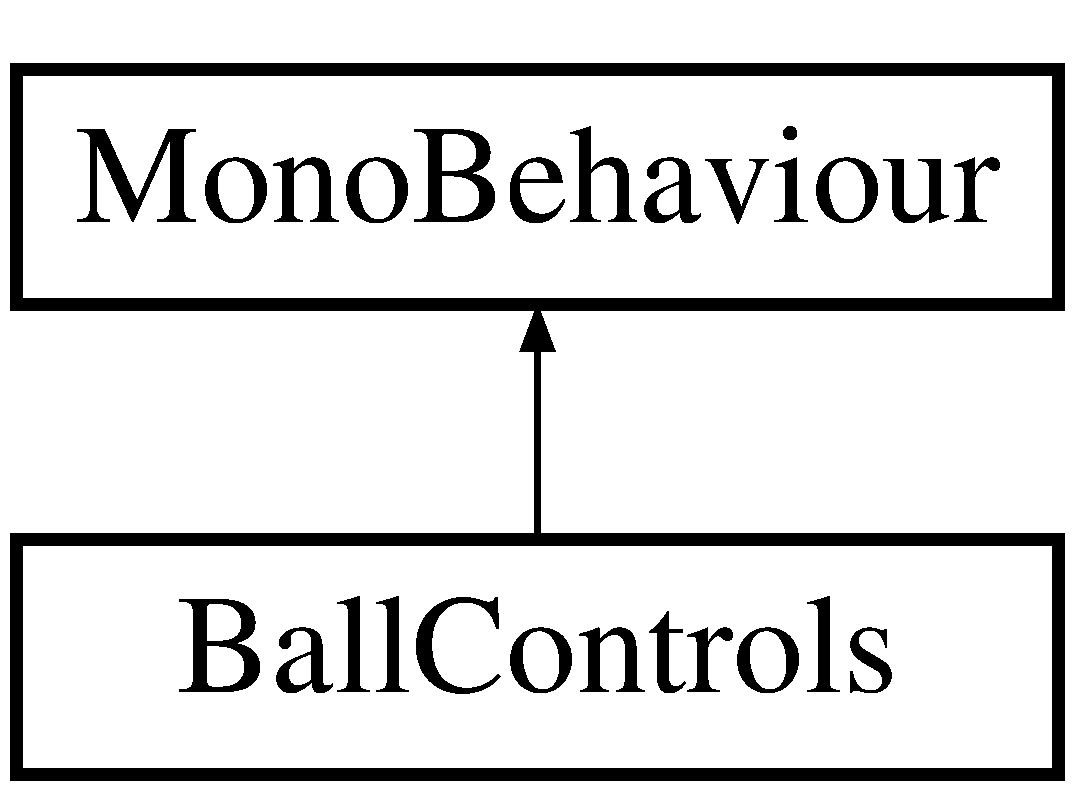
\includegraphics[height=2.000000cm]{class_ball_controls}
\end{center}
\end{figure}
\subsection*{Private Member Functions}
\begin{DoxyCompactItemize}
\item 
void \mbox{\hyperlink{class_ball_controls_afc951b5708e1230db03a9333c09a078a}{On\+Collision\+Enter}} (Collision col)
\item 
void \mbox{\hyperlink{class_ball_controls_a00d79b184e3653f025568ac5a9aeba20}{On\+Destroy}} ()
\end{DoxyCompactItemize}
\subsection*{Private Attributes}
\begin{DoxyCompactItemize}
\item 
Audio\+Source \mbox{\hyperlink{class_ball_controls_a8b478ef0dc12f8683cfdd7e485ee9d20}{Ball\+Sound\+Big}}
\item 
Audio\+Source \mbox{\hyperlink{class_ball_controls_acd4d5b722bd7ad4fd32d6df3cd9b5191}{Ball\+Sound\+Small}}
\end{DoxyCompactItemize}


\subsection{Member Function Documentation}
\mbox{\Hypertarget{class_ball_controls_afc951b5708e1230db03a9333c09a078a}\label{class_ball_controls_afc951b5708e1230db03a9333c09a078a}} 
\index{Ball\+Controls@{Ball\+Controls}!On\+Collision\+Enter@{On\+Collision\+Enter}}
\index{On\+Collision\+Enter@{On\+Collision\+Enter}!Ball\+Controls@{Ball\+Controls}}
\subsubsection{\texorpdfstring{On\+Collision\+Enter()}{OnCollisionEnter()}}
{\footnotesize\ttfamily void Ball\+Controls.\+On\+Collision\+Enter (\begin{DoxyParamCaption}\item[{Collision}]{col }\end{DoxyParamCaption})\hspace{0.3cm}{\ttfamily [private]}}

\mbox{\Hypertarget{class_ball_controls_a00d79b184e3653f025568ac5a9aeba20}\label{class_ball_controls_a00d79b184e3653f025568ac5a9aeba20}} 
\index{Ball\+Controls@{Ball\+Controls}!On\+Destroy@{On\+Destroy}}
\index{On\+Destroy@{On\+Destroy}!Ball\+Controls@{Ball\+Controls}}
\subsubsection{\texorpdfstring{On\+Destroy()}{OnDestroy()}}
{\footnotesize\ttfamily void Ball\+Controls.\+On\+Destroy (\begin{DoxyParamCaption}{ }\end{DoxyParamCaption})\hspace{0.3cm}{\ttfamily [private]}}



\subsection{Member Data Documentation}
\mbox{\Hypertarget{class_ball_controls_a8b478ef0dc12f8683cfdd7e485ee9d20}\label{class_ball_controls_a8b478ef0dc12f8683cfdd7e485ee9d20}} 
\index{Ball\+Controls@{Ball\+Controls}!Ball\+Sound\+Big@{Ball\+Sound\+Big}}
\index{Ball\+Sound\+Big@{Ball\+Sound\+Big}!Ball\+Controls@{Ball\+Controls}}
\subsubsection{\texorpdfstring{Ball\+Sound\+Big}{BallSoundBig}}
{\footnotesize\ttfamily Audio\+Source Ball\+Controls.\+Ball\+Sound\+Big\hspace{0.3cm}{\ttfamily [private]}}

\mbox{\Hypertarget{class_ball_controls_acd4d5b722bd7ad4fd32d6df3cd9b5191}\label{class_ball_controls_acd4d5b722bd7ad4fd32d6df3cd9b5191}} 
\index{Ball\+Controls@{Ball\+Controls}!Ball\+Sound\+Small@{Ball\+Sound\+Small}}
\index{Ball\+Sound\+Small@{Ball\+Sound\+Small}!Ball\+Controls@{Ball\+Controls}}
\subsubsection{\texorpdfstring{Ball\+Sound\+Small}{BallSoundSmall}}
{\footnotesize\ttfamily Audio\+Source Ball\+Controls.\+Ball\+Sound\+Small\hspace{0.3cm}{\ttfamily [private]}}



The documentation for this class was generated from the following file\+:\begin{DoxyCompactItemize}
\item 
\mbox{\hyperlink{_ball_controls_8cs}{Ball\+Controls.\+cs}}\end{DoxyCompactItemize}

\hypertarget{class_dialogue}{}\section{Dialogue Class Reference}
\label{class_dialogue}\index{Dialogue@{Dialogue}}


Creates a List of elements which contain attributes from \mbox{\hyperlink{_dialogue_element_8cs}{Dialogue\+Element.\+cs}}  


Inheritance diagram for Dialogue\+:\begin{figure}[H]
\begin{center}
\leavevmode
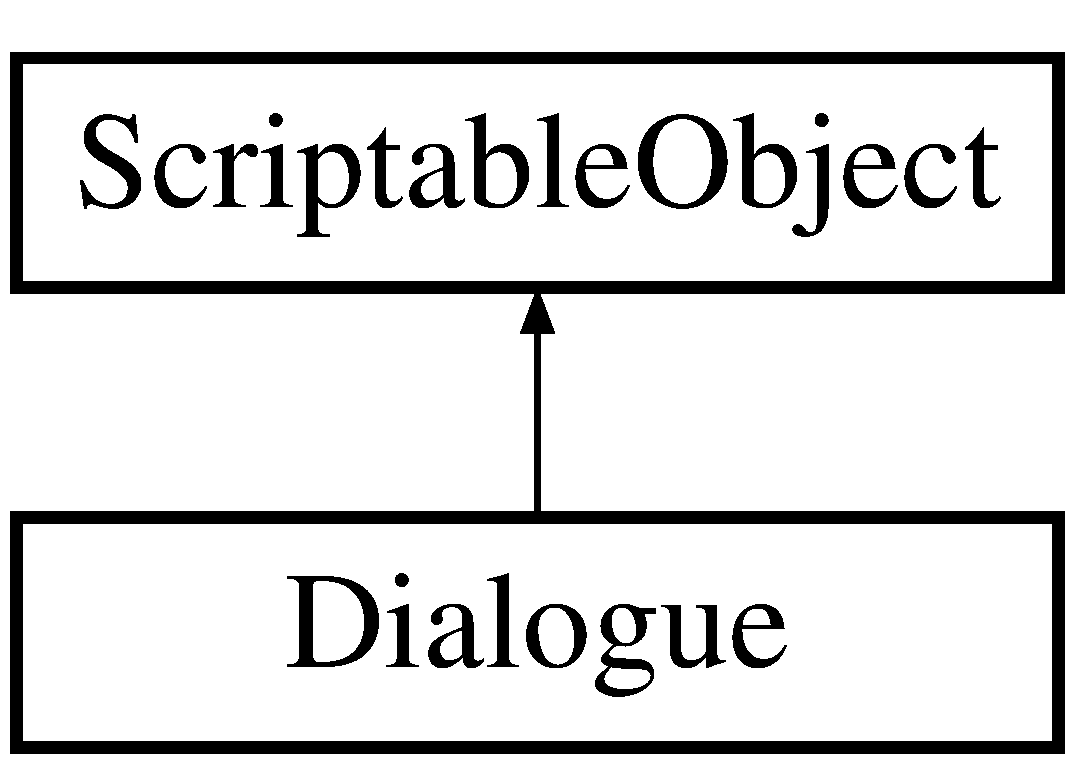
\includegraphics[height=2.000000cm]{class_dialogue}
\end{center}
\end{figure}
\subsection*{Public Attributes}
\begin{DoxyCompactItemize}
\item 
List$<$ \mbox{\hyperlink{class_dialogue_element}{Dialogue\+Element}} $>$ \mbox{\hyperlink{class_dialogue_ae24b80e9ccce4796c937901ba0db94c4}{Dialogue\+Elements}} = new List$<$\mbox{\hyperlink{class_dialogue_element}{Dialogue\+Element}}$>$()
\end{DoxyCompactItemize}


\subsection{Detailed Description}
Creates a List of elements which contain attributes from \mbox{\hyperlink{_dialogue_element_8cs}{Dialogue\+Element.\+cs}} 



\subsection{Member Data Documentation}
\mbox{\Hypertarget{class_dialogue_ae24b80e9ccce4796c937901ba0db94c4}\label{class_dialogue_ae24b80e9ccce4796c937901ba0db94c4}} 
\index{Dialogue@{Dialogue}!Dialogue\+Elements@{Dialogue\+Elements}}
\index{Dialogue\+Elements@{Dialogue\+Elements}!Dialogue@{Dialogue}}
\subsubsection{\texorpdfstring{Dialogue\+Elements}{DialogueElements}}
{\footnotesize\ttfamily List$<$\mbox{\hyperlink{class_dialogue_element}{Dialogue\+Element}}$>$ Dialogue.\+Dialogue\+Elements = new List$<$\mbox{\hyperlink{class_dialogue_element}{Dialogue\+Element}}$>$()}



The documentation for this class was generated from the following file\+:\begin{DoxyCompactItemize}
\item 
Dialogue/scripts/\mbox{\hyperlink{_dialogue_8cs}{Dialogue.\+cs}}\end{DoxyCompactItemize}

\hypertarget{class_dialogue_asset}{}\section{Dialogue\+Asset Class Reference}
\label{class_dialogue_asset}\index{Dialogue\+Asset@{Dialogue\+Asset}}


Overload the menu for creating a custom \mbox{\hyperlink{class_dialogue}{Dialogue}} asset.  


\subsection*{Static Public Member Functions}
\begin{DoxyCompactItemize}
\item 
static void \mbox{\hyperlink{class_dialogue_asset_a3f5b610dda86b22834c2429a926e8bd0}{Create\+Asset}} ()
\end{DoxyCompactItemize}


\subsection{Detailed Description}
Overload the menu for creating a custom \mbox{\hyperlink{class_dialogue}{Dialogue}} asset. 



\subsection{Member Function Documentation}
\mbox{\Hypertarget{class_dialogue_asset_a3f5b610dda86b22834c2429a926e8bd0}\label{class_dialogue_asset_a3f5b610dda86b22834c2429a926e8bd0}} 
\index{Dialogue\+Asset@{Dialogue\+Asset}!Create\+Asset@{Create\+Asset}}
\index{Create\+Asset@{Create\+Asset}!Dialogue\+Asset@{Dialogue\+Asset}}
\subsubsection{\texorpdfstring{Create\+Asset()}{CreateAsset()}}
{\footnotesize\ttfamily static void Dialogue\+Asset.\+Create\+Asset (\begin{DoxyParamCaption}{ }\end{DoxyParamCaption})\hspace{0.3cm}{\ttfamily [static]}}



The documentation for this class was generated from the following file\+:\begin{DoxyCompactItemize}
\item 
Dialogue/\+Editor/\mbox{\hyperlink{_dialogue_asset_8cs}{Dialogue\+Asset.\+cs}}\end{DoxyCompactItemize}

\hypertarget{class_dialogue_editor}{}\section{Dialogue\+Editor Class Reference}
\label{class_dialogue_editor}\index{Dialogue\+Editor@{Dialogue\+Editor}}


Tells Unity that we can handle the editor view ourself.  


Inheritance diagram for Dialogue\+Editor\+:\begin{figure}[H]
\begin{center}
\leavevmode
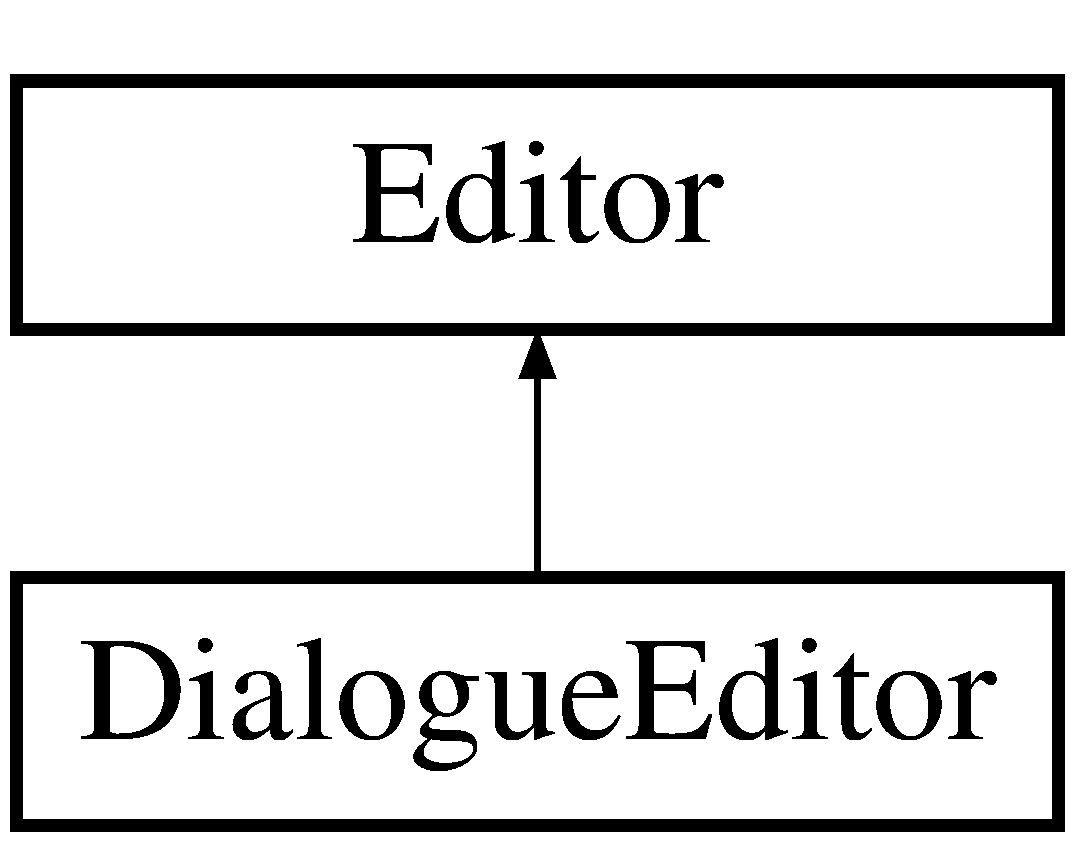
\includegraphics[height=2.000000cm]{class_dialogue_editor}
\end{center}
\end{figure}
\subsection*{Public Member Functions}
\begin{DoxyCompactItemize}
\item 
override void \mbox{\hyperlink{class_dialogue_editor_ad36b3f14a8f1f1a9d71c716751e9e889}{On\+Inspector\+G\+UI}} ()
\begin{DoxyCompactList}\small\item\em Overides the custom inspector view for our \mbox{\hyperlink{class_dialogue}{Dialogue}} Elements. \end{DoxyCompactList}\end{DoxyCompactItemize}
\subsection*{Private Member Functions}
\begin{DoxyCompactItemize}
\item 
void \mbox{\hyperlink{class_dialogue_editor_a021f39e2fd0e5ba4c1d325785e73e073}{On\+Enable}} ()
\item 
string \mbox{\hyperlink{class_dialogue_editor_a7c45fc0781ade3441db9948bc4b3ec39}{Get\+Text\+Area}} (\mbox{\hyperlink{class_dialogue_element}{Dialogue\+Element}} elm)
\begin{DoxyCompactList}\small\item\em Creates the dialogue text area to edit text. \end{DoxyCompactList}\item 
Texture2D \mbox{\hyperlink{class_dialogue_editor_a797c90eb2333c7e9421917ecef6da189}{Get\+Char\+Pic}} (string name, Texture2D texture)
\begin{DoxyCompactList}\small\item\em Creates the N\+PC image area if we wanted to display a picture of who is talking. \end{DoxyCompactList}\item 
\mbox{\hyperlink{class_dialogue_element_ae49b75aacbe9e237b4801a4153dd1bfa}{Dialogue\+Element.\+Characters}} \mbox{\hyperlink{class_dialogue_editor_a9bc812d2ac0daea075c7c6d408a524dd}{Select\+N\+PC}} (\mbox{\hyperlink{class_dialogue_element}{Dialogue\+Element}} elm)
\begin{DoxyCompactList}\small\item\em Choose which N\+PC is talking via drop down menu \end{DoxyCompactList}\item 
\mbox{\hyperlink{class_dialogue_element_a4713e15d24a53d5487f1d51b89cd55ee}{Dialogue\+Element.\+Avatar\+Pos}} \mbox{\hyperlink{class_dialogue_editor_a91ae346ba8ec20e732d1dfc3eb12aad4}{Select\+Pos}} (\mbox{\hyperlink{class_dialogue_element}{Dialogue\+Element}} elm)
\begin{DoxyCompactList}\small\item\em Choose position of N\+PC image position. \end{DoxyCompactList}\item 
Audio\+Clip \mbox{\hyperlink{class_dialogue_editor_a004ee96b1b14c0daab83f8ca66af7d60}{Select\+Audio\+Clip}} (\mbox{\hyperlink{class_dialogue_element}{Dialogue\+Element}} elm)
\begin{DoxyCompactList}\small\item\em Set audio clip for the dialogue if the N\+PC is speaking. \end{DoxyCompactList}\item 
int \mbox{\hyperlink{class_dialogue_editor_a4f9858a733113b0dab1177ac806a43d0}{Remove\+Element}} (int \mbox{\hyperlink{class_dialogue_editor_a283d0bf74d897ae870ad3bdc7c7dcd2a}{index}})
\begin{DoxyCompactList}\small\item\em Function for removing elements at a specified index. \end{DoxyCompactList}\end{DoxyCompactItemize}
\subsection*{Private Attributes}
\begin{DoxyCompactItemize}
\item 
\mbox{\hyperlink{class_dialogue}{Dialogue}} \mbox{\hyperlink{class_dialogue_editor_aa05e8f2205c153236f9d2ce81b4857c3}{D}}
\item 
int \mbox{\hyperlink{class_dialogue_editor_a283d0bf74d897ae870ad3bdc7c7dcd2a}{index}} = 0
\end{DoxyCompactItemize}


\subsection{Detailed Description}
Tells Unity that we can handle the editor view ourself. 



\subsection{Member Function Documentation}
\mbox{\Hypertarget{class_dialogue_editor_a797c90eb2333c7e9421917ecef6da189}\label{class_dialogue_editor_a797c90eb2333c7e9421917ecef6da189}} 
\index{Dialogue\+Editor@{Dialogue\+Editor}!Get\+Char\+Pic@{Get\+Char\+Pic}}
\index{Get\+Char\+Pic@{Get\+Char\+Pic}!Dialogue\+Editor@{Dialogue\+Editor}}
\subsubsection{\texorpdfstring{Get\+Char\+Pic()}{GetCharPic()}}
{\footnotesize\ttfamily Texture2D Dialogue\+Editor.\+Get\+Char\+Pic (\begin{DoxyParamCaption}\item[{string}]{name,  }\item[{Texture2D}]{texture }\end{DoxyParamCaption})\hspace{0.3cm}{\ttfamily [private]}}



Creates the N\+PC image area if we wanted to display a picture of who is talking. 


\begin{DoxyParams}{Parameters}
{\em name} & Name of the character talking.\\
\hline
{\em texture} & Picture of the character talking.\\
\hline
\end{DoxyParams}
\begin{DoxyReturn}{Returns}
Returns a texture box for dragging in an image.
\end{DoxyReturn}
\mbox{\Hypertarget{class_dialogue_editor_a7c45fc0781ade3441db9948bc4b3ec39}\label{class_dialogue_editor_a7c45fc0781ade3441db9948bc4b3ec39}} 
\index{Dialogue\+Editor@{Dialogue\+Editor}!Get\+Text\+Area@{Get\+Text\+Area}}
\index{Get\+Text\+Area@{Get\+Text\+Area}!Dialogue\+Editor@{Dialogue\+Editor}}
\subsubsection{\texorpdfstring{Get\+Text\+Area()}{GetTextArea()}}
{\footnotesize\ttfamily string Dialogue\+Editor.\+Get\+Text\+Area (\begin{DoxyParamCaption}\item[{\mbox{\hyperlink{class_dialogue_element}{Dialogue\+Element}}}]{elm }\end{DoxyParamCaption})\hspace{0.3cm}{\ttfamily [private]}}



Creates the dialogue text area to edit text. 


\begin{DoxyParams}{Parameters}
{\em elm} & For each element give it a text box and label for the text.\\
\hline
\end{DoxyParams}
\begin{DoxyReturn}{Returns}
Returns the text area box with a label.
\end{DoxyReturn}
\mbox{\Hypertarget{class_dialogue_editor_a021f39e2fd0e5ba4c1d325785e73e073}\label{class_dialogue_editor_a021f39e2fd0e5ba4c1d325785e73e073}} 
\index{Dialogue\+Editor@{Dialogue\+Editor}!On\+Enable@{On\+Enable}}
\index{On\+Enable@{On\+Enable}!Dialogue\+Editor@{Dialogue\+Editor}}
\subsubsection{\texorpdfstring{On\+Enable()}{OnEnable()}}
{\footnotesize\ttfamily void Dialogue\+Editor.\+On\+Enable (\begin{DoxyParamCaption}{ }\end{DoxyParamCaption})\hspace{0.3cm}{\ttfamily [private]}}

\mbox{\Hypertarget{class_dialogue_editor_ad36b3f14a8f1f1a9d71c716751e9e889}\label{class_dialogue_editor_ad36b3f14a8f1f1a9d71c716751e9e889}} 
\index{Dialogue\+Editor@{Dialogue\+Editor}!On\+Inspector\+G\+UI@{On\+Inspector\+G\+UI}}
\index{On\+Inspector\+G\+UI@{On\+Inspector\+G\+UI}!Dialogue\+Editor@{Dialogue\+Editor}}
\subsubsection{\texorpdfstring{On\+Inspector\+G\+U\+I()}{OnInspectorGUI()}}
{\footnotesize\ttfamily override void Dialogue\+Editor.\+On\+Inspector\+G\+UI (\begin{DoxyParamCaption}{ }\end{DoxyParamCaption})}



Overides the custom inspector view for our \mbox{\hyperlink{class_dialogue}{Dialogue}} Elements. 

\mbox{\Hypertarget{class_dialogue_editor_a4f9858a733113b0dab1177ac806a43d0}\label{class_dialogue_editor_a4f9858a733113b0dab1177ac806a43d0}} 
\index{Dialogue\+Editor@{Dialogue\+Editor}!Remove\+Element@{Remove\+Element}}
\index{Remove\+Element@{Remove\+Element}!Dialogue\+Editor@{Dialogue\+Editor}}
\subsubsection{\texorpdfstring{Remove\+Element()}{RemoveElement()}}
{\footnotesize\ttfamily int Dialogue\+Editor.\+Remove\+Element (\begin{DoxyParamCaption}\item[{int}]{index }\end{DoxyParamCaption})\hspace{0.3cm}{\ttfamily [private]}}



Function for removing elements at a specified index. 


\begin{DoxyParams}{Parameters}
{\em index} & Specified index for removing an element from a list at any index.\\
\hline
\end{DoxyParams}
\begin{DoxyReturn}{Returns}
Returns the index specified in the int field
\end{DoxyReturn}
\mbox{\Hypertarget{class_dialogue_editor_a004ee96b1b14c0daab83f8ca66af7d60}\label{class_dialogue_editor_a004ee96b1b14c0daab83f8ca66af7d60}} 
\index{Dialogue\+Editor@{Dialogue\+Editor}!Select\+Audio\+Clip@{Select\+Audio\+Clip}}
\index{Select\+Audio\+Clip@{Select\+Audio\+Clip}!Dialogue\+Editor@{Dialogue\+Editor}}
\subsubsection{\texorpdfstring{Select\+Audio\+Clip()}{SelectAudioClip()}}
{\footnotesize\ttfamily Audio\+Clip Dialogue\+Editor.\+Select\+Audio\+Clip (\begin{DoxyParamCaption}\item[{\mbox{\hyperlink{class_dialogue_element}{Dialogue\+Element}}}]{elm }\end{DoxyParamCaption})\hspace{0.3cm}{\ttfamily [private]}}



Set audio clip for the dialogue if the N\+PC is speaking. 


\begin{DoxyParams}{Parameters}
{\em elm} & For each element give it an audio clip associated with the text.\\
\hline
\end{DoxyParams}
\begin{DoxyReturn}{Returns}
Returns a object box for dragging in an audio clip.
\end{DoxyReturn}
\mbox{\Hypertarget{class_dialogue_editor_a9bc812d2ac0daea075c7c6d408a524dd}\label{class_dialogue_editor_a9bc812d2ac0daea075c7c6d408a524dd}} 
\index{Dialogue\+Editor@{Dialogue\+Editor}!Select\+N\+PC@{Select\+N\+PC}}
\index{Select\+N\+PC@{Select\+N\+PC}!Dialogue\+Editor@{Dialogue\+Editor}}
\subsubsection{\texorpdfstring{Select\+N\+P\+C()}{SelectNPC()}}
{\footnotesize\ttfamily \mbox{\hyperlink{class_dialogue_element_ae49b75aacbe9e237b4801a4153dd1bfa}{Dialogue\+Element.\+Characters}} Dialogue\+Editor.\+Select\+N\+PC (\begin{DoxyParamCaption}\item[{\mbox{\hyperlink{class_dialogue_element}{Dialogue\+Element}}}]{elm }\end{DoxyParamCaption})\hspace{0.3cm}{\ttfamily [private]}}



Choose which N\+PC is talking via drop down menu 


\begin{DoxyParams}{Parameters}
{\em elm} & For each element give it a drop down menu for selecting the character associated with the text and audio. \\
\hline
\end{DoxyParams}
\begin{DoxyReturn}{Returns}
Returns a dropdown box for the N\+PC
\end{DoxyReturn}
\mbox{\Hypertarget{class_dialogue_editor_a91ae346ba8ec20e732d1dfc3eb12aad4}\label{class_dialogue_editor_a91ae346ba8ec20e732d1dfc3eb12aad4}} 
\index{Dialogue\+Editor@{Dialogue\+Editor}!Select\+Pos@{Select\+Pos}}
\index{Select\+Pos@{Select\+Pos}!Dialogue\+Editor@{Dialogue\+Editor}}
\subsubsection{\texorpdfstring{Select\+Pos()}{SelectPos()}}
{\footnotesize\ttfamily \mbox{\hyperlink{class_dialogue_element_a4713e15d24a53d5487f1d51b89cd55ee}{Dialogue\+Element.\+Avatar\+Pos}} Dialogue\+Editor.\+Select\+Pos (\begin{DoxyParamCaption}\item[{\mbox{\hyperlink{class_dialogue_element}{Dialogue\+Element}}}]{elm }\end{DoxyParamCaption})\hspace{0.3cm}{\ttfamily [private]}}



Choose position of N\+PC image position. 


\begin{DoxyParams}{Parameters}
{\em elm} & For each element give it a position to put the N\+PC image.\\
\hline
\end{DoxyParams}
\begin{DoxyReturn}{Returns}
Returns a drop down menu for selecting the position of the character.
\end{DoxyReturn}


\subsection{Member Data Documentation}
\mbox{\Hypertarget{class_dialogue_editor_aa05e8f2205c153236f9d2ce81b4857c3}\label{class_dialogue_editor_aa05e8f2205c153236f9d2ce81b4857c3}} 
\index{Dialogue\+Editor@{Dialogue\+Editor}!D@{D}}
\index{D@{D}!Dialogue\+Editor@{Dialogue\+Editor}}
\subsubsection{\texorpdfstring{D}{D}}
{\footnotesize\ttfamily \mbox{\hyperlink{class_dialogue}{Dialogue}} Dialogue\+Editor.\+D\hspace{0.3cm}{\ttfamily [private]}}

\mbox{\Hypertarget{class_dialogue_editor_a283d0bf74d897ae870ad3bdc7c7dcd2a}\label{class_dialogue_editor_a283d0bf74d897ae870ad3bdc7c7dcd2a}} 
\index{Dialogue\+Editor@{Dialogue\+Editor}!index@{index}}
\index{index@{index}!Dialogue\+Editor@{Dialogue\+Editor}}
\subsubsection{\texorpdfstring{index}{index}}
{\footnotesize\ttfamily int Dialogue\+Editor.\+index = 0\hspace{0.3cm}{\ttfamily [private]}}



The documentation for this class was generated from the following file\+:\begin{DoxyCompactItemize}
\item 
Dialogue/\+Editor/\mbox{\hyperlink{_dialogue_editor_8cs}{Dialogue\+Editor.\+cs}}\end{DoxyCompactItemize}

\hypertarget{class_dialogue_element}{}\section{Dialogue\+Element Class Reference}
\label{class_dialogue_element}\index{Dialogue\+Element@{Dialogue\+Element}}


This is where you can add attributes to each dialogue element instance. Note some of this wasn\textquotesingle{}t used or included in the \mbox{\hyperlink{class_dialogue_editor}{Dialogue\+Editor}} view under Project $>$ \mbox{\hyperlink{class_dialogue}{Dialogue}} $>$ Editor...  


\subsection*{Public Types}
\begin{DoxyCompactItemize}
\item 
enum \mbox{\hyperlink{class_dialogue_element_ae49b75aacbe9e237b4801a4153dd1bfa}{Characters}} \{ \mbox{\hyperlink{class_dialogue_element_ae49b75aacbe9e237b4801a4153dd1bfaa5d1eca158c00250d9c4c32d947b7c433}{Characters.\+Robot}}
 \}
\item 
enum \mbox{\hyperlink{class_dialogue_element_a4713e15d24a53d5487f1d51b89cd55ee}{Avatar\+Pos}} \{ \mbox{\hyperlink{class_dialogue_element_a4713e15d24a53d5487f1d51b89cd55eea811882fecd5c7618d7099ebbd39ea254}{Avatar\+Pos.\+left}}, 
\mbox{\hyperlink{class_dialogue_element_a4713e15d24a53d5487f1d51b89cd55eea7c4f29407893c334a6cb7a87bf045c0d}{Avatar\+Pos.\+right}}
 \}
\end{DoxyCompactItemize}
\subsection*{Public Attributes}
\begin{DoxyCompactItemize}
\item 
\mbox{\hyperlink{class_dialogue_element_ae49b75aacbe9e237b4801a4153dd1bfa}{Characters}} \mbox{\hyperlink{class_dialogue_element_ab41891d5d0d2f140ef8cb70cd2471e9c}{Character}}
\item 
\mbox{\hyperlink{class_dialogue_element_a4713e15d24a53d5487f1d51b89cd55ee}{Avatar\+Pos}} \mbox{\hyperlink{class_dialogue_element_ab77dcc6f1586a68b72a1d2d9dfca3b50}{Character\+Pos}}
\item 
Texture2D \mbox{\hyperlink{class_dialogue_element_a65e82dcc1e979f6890fd1f0c08cd43a6}{Character\+Pic}}
\item 
string \mbox{\hyperlink{class_dialogue_element_aa2557c80fc22e7327fb48a02991024de}{Dialogue\+Text}}
\item 
G\+U\+I\+Style \mbox{\hyperlink{class_dialogue_element_ad4d43ed3aa5816446241e93d59ebf409}{Dialogue\+Text\+Style}}
\item 
float \mbox{\hyperlink{class_dialogue_element_a14e05abcef33f93b97d5b3ae2c11dd1d}{Text\+Play\+Back\+Speed}}
\item 
Audio\+Clip \mbox{\hyperlink{class_dialogue_element_a39327338f1eff135aa4f3c258098cb8a}{Play\+Back\+Sound\+File}}
\end{DoxyCompactItemize}


\subsection{Detailed Description}
This is where you can add attributes to each dialogue element instance. Note some of this wasn\textquotesingle{}t used or included in the \mbox{\hyperlink{class_dialogue_editor}{Dialogue\+Editor}} view under Project $>$ \mbox{\hyperlink{class_dialogue}{Dialogue}} $>$ Editor... 



\subsection{Member Enumeration Documentation}
\mbox{\Hypertarget{class_dialogue_element_a4713e15d24a53d5487f1d51b89cd55ee}\label{class_dialogue_element_a4713e15d24a53d5487f1d51b89cd55ee}} 
\index{Dialogue\+Element@{Dialogue\+Element}!Avatar\+Pos@{Avatar\+Pos}}
\index{Avatar\+Pos@{Avatar\+Pos}!Dialogue\+Element@{Dialogue\+Element}}
\subsubsection{\texorpdfstring{Avatar\+Pos}{AvatarPos}}
{\footnotesize\ttfamily enum \mbox{\hyperlink{class_dialogue_element_a4713e15d24a53d5487f1d51b89cd55ee}{Dialogue\+Element.\+Avatar\+Pos}}\hspace{0.3cm}{\ttfamily [strong]}}

\begin{DoxyEnumFields}{Enumerator}
\raisebox{\heightof{T}}[0pt][0pt]{\index{left@{left}!Dialogue\+Element@{Dialogue\+Element}}\index{Dialogue\+Element@{Dialogue\+Element}!left@{left}}}\mbox{\Hypertarget{class_dialogue_element_a4713e15d24a53d5487f1d51b89cd55eea811882fecd5c7618d7099ebbd39ea254}\label{class_dialogue_element_a4713e15d24a53d5487f1d51b89cd55eea811882fecd5c7618d7099ebbd39ea254}} 
left&\\
\hline

\raisebox{\heightof{T}}[0pt][0pt]{\index{right@{right}!Dialogue\+Element@{Dialogue\+Element}}\index{Dialogue\+Element@{Dialogue\+Element}!right@{right}}}\mbox{\Hypertarget{class_dialogue_element_a4713e15d24a53d5487f1d51b89cd55eea7c4f29407893c334a6cb7a87bf045c0d}\label{class_dialogue_element_a4713e15d24a53d5487f1d51b89cd55eea7c4f29407893c334a6cb7a87bf045c0d}} 
right&\\
\hline

\end{DoxyEnumFields}
\mbox{\Hypertarget{class_dialogue_element_ae49b75aacbe9e237b4801a4153dd1bfa}\label{class_dialogue_element_ae49b75aacbe9e237b4801a4153dd1bfa}} 
\index{Dialogue\+Element@{Dialogue\+Element}!Characters@{Characters}}
\index{Characters@{Characters}!Dialogue\+Element@{Dialogue\+Element}}
\subsubsection{\texorpdfstring{Characters}{Characters}}
{\footnotesize\ttfamily enum \mbox{\hyperlink{class_dialogue_element_ae49b75aacbe9e237b4801a4153dd1bfa}{Dialogue\+Element.\+Characters}}\hspace{0.3cm}{\ttfamily [strong]}}

\begin{DoxyEnumFields}{Enumerator}
\raisebox{\heightof{T}}[0pt][0pt]{\index{Robot@{Robot}!Dialogue\+Element@{Dialogue\+Element}}\index{Dialogue\+Element@{Dialogue\+Element}!Robot@{Robot}}}\mbox{\Hypertarget{class_dialogue_element_ae49b75aacbe9e237b4801a4153dd1bfaa5d1eca158c00250d9c4c32d947b7c433}\label{class_dialogue_element_ae49b75aacbe9e237b4801a4153dd1bfaa5d1eca158c00250d9c4c32d947b7c433}} 
Robot&\\
\hline

\end{DoxyEnumFields}


\subsection{Member Data Documentation}
\mbox{\Hypertarget{class_dialogue_element_ab41891d5d0d2f140ef8cb70cd2471e9c}\label{class_dialogue_element_ab41891d5d0d2f140ef8cb70cd2471e9c}} 
\index{Dialogue\+Element@{Dialogue\+Element}!Character@{Character}}
\index{Character@{Character}!Dialogue\+Element@{Dialogue\+Element}}
\subsubsection{\texorpdfstring{Character}{Character}}
{\footnotesize\ttfamily \mbox{\hyperlink{class_dialogue_element_ae49b75aacbe9e237b4801a4153dd1bfa}{Characters}} Dialogue\+Element.\+Character}

\mbox{\Hypertarget{class_dialogue_element_a65e82dcc1e979f6890fd1f0c08cd43a6}\label{class_dialogue_element_a65e82dcc1e979f6890fd1f0c08cd43a6}} 
\index{Dialogue\+Element@{Dialogue\+Element}!Character\+Pic@{Character\+Pic}}
\index{Character\+Pic@{Character\+Pic}!Dialogue\+Element@{Dialogue\+Element}}
\subsubsection{\texorpdfstring{Character\+Pic}{CharacterPic}}
{\footnotesize\ttfamily Texture2D Dialogue\+Element.\+Character\+Pic}

\mbox{\Hypertarget{class_dialogue_element_ab77dcc6f1586a68b72a1d2d9dfca3b50}\label{class_dialogue_element_ab77dcc6f1586a68b72a1d2d9dfca3b50}} 
\index{Dialogue\+Element@{Dialogue\+Element}!Character\+Pos@{Character\+Pos}}
\index{Character\+Pos@{Character\+Pos}!Dialogue\+Element@{Dialogue\+Element}}
\subsubsection{\texorpdfstring{Character\+Pos}{CharacterPos}}
{\footnotesize\ttfamily \mbox{\hyperlink{class_dialogue_element_a4713e15d24a53d5487f1d51b89cd55ee}{Avatar\+Pos}} Dialogue\+Element.\+Character\+Pos}

\mbox{\Hypertarget{class_dialogue_element_aa2557c80fc22e7327fb48a02991024de}\label{class_dialogue_element_aa2557c80fc22e7327fb48a02991024de}} 
\index{Dialogue\+Element@{Dialogue\+Element}!Dialogue\+Text@{Dialogue\+Text}}
\index{Dialogue\+Text@{Dialogue\+Text}!Dialogue\+Element@{Dialogue\+Element}}
\subsubsection{\texorpdfstring{Dialogue\+Text}{DialogueText}}
{\footnotesize\ttfamily string Dialogue\+Element.\+Dialogue\+Text}

\mbox{\Hypertarget{class_dialogue_element_ad4d43ed3aa5816446241e93d59ebf409}\label{class_dialogue_element_ad4d43ed3aa5816446241e93d59ebf409}} 
\index{Dialogue\+Element@{Dialogue\+Element}!Dialogue\+Text\+Style@{Dialogue\+Text\+Style}}
\index{Dialogue\+Text\+Style@{Dialogue\+Text\+Style}!Dialogue\+Element@{Dialogue\+Element}}
\subsubsection{\texorpdfstring{Dialogue\+Text\+Style}{DialogueTextStyle}}
{\footnotesize\ttfamily G\+U\+I\+Style Dialogue\+Element.\+Dialogue\+Text\+Style}

\mbox{\Hypertarget{class_dialogue_element_a39327338f1eff135aa4f3c258098cb8a}\label{class_dialogue_element_a39327338f1eff135aa4f3c258098cb8a}} 
\index{Dialogue\+Element@{Dialogue\+Element}!Play\+Back\+Sound\+File@{Play\+Back\+Sound\+File}}
\index{Play\+Back\+Sound\+File@{Play\+Back\+Sound\+File}!Dialogue\+Element@{Dialogue\+Element}}
\subsubsection{\texorpdfstring{Play\+Back\+Sound\+File}{PlayBackSoundFile}}
{\footnotesize\ttfamily Audio\+Clip Dialogue\+Element.\+Play\+Back\+Sound\+File}

\mbox{\Hypertarget{class_dialogue_element_a14e05abcef33f93b97d5b3ae2c11dd1d}\label{class_dialogue_element_a14e05abcef33f93b97d5b3ae2c11dd1d}} 
\index{Dialogue\+Element@{Dialogue\+Element}!Text\+Play\+Back\+Speed@{Text\+Play\+Back\+Speed}}
\index{Text\+Play\+Back\+Speed@{Text\+Play\+Back\+Speed}!Dialogue\+Element@{Dialogue\+Element}}
\subsubsection{\texorpdfstring{Text\+Play\+Back\+Speed}{TextPlayBackSpeed}}
{\footnotesize\ttfamily float Dialogue\+Element.\+Text\+Play\+Back\+Speed}



The documentation for this class was generated from the following file\+:\begin{DoxyCompactItemize}
\item 
Dialogue/scripts/\mbox{\hyperlink{_dialogue_element_8cs}{Dialogue\+Element.\+cs}}\end{DoxyCompactItemize}

\hypertarget{class_end_scene}{}\section{End\+Scene Class Reference}
\label{class_end_scene}\index{End\+Scene@{End\+Scene}}
Inheritance diagram for End\+Scene\+:\begin{figure}[H]
\begin{center}
\leavevmode
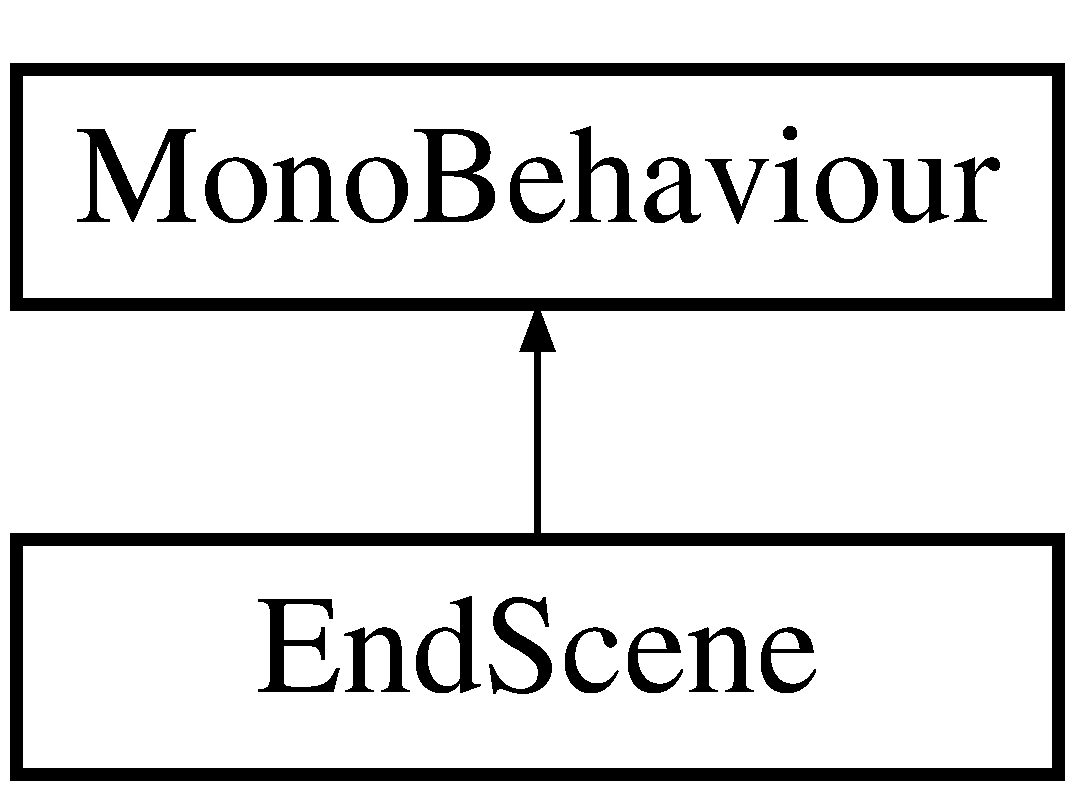
\includegraphics[height=2.000000cm]{class_end_scene}
\end{center}
\end{figure}
\subsection*{Static Public Attributes}
\begin{DoxyCompactItemize}
\item 
static \mbox{\hyperlink{class_end_scene}{End\+Scene}} \mbox{\hyperlink{class_end_scene_a6cf08b038600652991ae00a9cf2a949b}{s\+\_\+\+Instance}} = null
\end{DoxyCompactItemize}
\subsection*{Private Member Functions}
\begin{DoxyCompactItemize}
\item 
void \mbox{\hyperlink{class_end_scene_af546101a56df683a50f88f6809d4638a}{Start}} ()
\item 
I\+Enumerator \mbox{\hyperlink{class_end_scene_aad3f8f074f1937a0615f21e95b74f33c}{Run}} ()
\begin{DoxyCompactList}\small\item\em Controls the flow of the scene. \end{DoxyCompactList}\item 
I\+Enumerator \mbox{\hyperlink{class_end_scene_aee3c069e59445bbd2c6cfa69f498fead}{Fading\+Out}} ()
\begin{DoxyCompactList}\small\item\em Two animations\+: but Fading\+In is a transparent image \end{DoxyCompactList}\end{DoxyCompactItemize}
\subsection*{Private Attributes}
\begin{DoxyCompactItemize}
\item 
\mbox{\hyperlink{class_intro_session_manager}{Intro\+Session\+Manager}} \mbox{\hyperlink{class_end_scene_a55d85fe74c61b09ec0bbf2f8eb6a7a43}{m\+\_\+\+Manager}}
\item 
\mbox{\hyperlink{class_dialogue}{Dialogue}} \mbox{\hyperlink{class_end_scene_ae1a4aeefdb40b81df7d910bfb7c909b9}{m\+\_\+\+Dialogue\+Instructions}}
\item 
Game\+Object \mbox{\hyperlink{class_end_scene_a2b10ad0874c9ad181f1dd93d93bd246a}{m\+\_\+\+Robot\+End\+Position}}
\item 
Image \mbox{\hyperlink{class_end_scene_a9b30c59b3252565d3b2bf3de29fe4403}{m\+\_\+\+Black}}
\item 
Animator \mbox{\hyperlink{class_end_scene_a85e334f53cb4f5b9b44c499b5224cc62}{m\+\_\+\+Anim}}
\end{DoxyCompactItemize}


\subsection{Member Function Documentation}
\mbox{\Hypertarget{class_end_scene_aee3c069e59445bbd2c6cfa69f498fead}\label{class_end_scene_aee3c069e59445bbd2c6cfa69f498fead}} 
\index{End\+Scene@{End\+Scene}!Fading\+Out@{Fading\+Out}}
\index{Fading\+Out@{Fading\+Out}!End\+Scene@{End\+Scene}}
\subsubsection{\texorpdfstring{Fading\+Out()}{FadingOut()}}
{\footnotesize\ttfamily I\+Enumerator End\+Scene.\+Fading\+Out (\begin{DoxyParamCaption}{ }\end{DoxyParamCaption})\hspace{0.3cm}{\ttfamily [private]}}



Two animations\+: but Fading\+In is a transparent image 

\begin{DoxyReturn}{Returns}
A reference to the coroutine
\end{DoxyReturn}
\mbox{\Hypertarget{class_end_scene_aad3f8f074f1937a0615f21e95b74f33c}\label{class_end_scene_aad3f8f074f1937a0615f21e95b74f33c}} 
\index{End\+Scene@{End\+Scene}!Run@{Run}}
\index{Run@{Run}!End\+Scene@{End\+Scene}}
\subsubsection{\texorpdfstring{Run()}{Run()}}
{\footnotesize\ttfamily I\+Enumerator End\+Scene.\+Run (\begin{DoxyParamCaption}{ }\end{DoxyParamCaption})\hspace{0.3cm}{\ttfamily [private]}}



Controls the flow of the scene. 

\begin{DoxyReturn}{Returns}
A reference to the coroutine
\end{DoxyReturn}
\mbox{\Hypertarget{class_end_scene_af546101a56df683a50f88f6809d4638a}\label{class_end_scene_af546101a56df683a50f88f6809d4638a}} 
\index{End\+Scene@{End\+Scene}!Start@{Start}}
\index{Start@{Start}!End\+Scene@{End\+Scene}}
\subsubsection{\texorpdfstring{Start()}{Start()}}
{\footnotesize\ttfamily void End\+Scene.\+Start (\begin{DoxyParamCaption}{ }\end{DoxyParamCaption})\hspace{0.3cm}{\ttfamily [private]}}



\subsection{Member Data Documentation}
\mbox{\Hypertarget{class_end_scene_a85e334f53cb4f5b9b44c499b5224cc62}\label{class_end_scene_a85e334f53cb4f5b9b44c499b5224cc62}} 
\index{End\+Scene@{End\+Scene}!m\+\_\+\+Anim@{m\+\_\+\+Anim}}
\index{m\+\_\+\+Anim@{m\+\_\+\+Anim}!End\+Scene@{End\+Scene}}
\subsubsection{\texorpdfstring{m\+\_\+\+Anim}{m\_Anim}}
{\footnotesize\ttfamily Animator End\+Scene.\+m\+\_\+\+Anim\hspace{0.3cm}{\ttfamily [private]}}

\mbox{\Hypertarget{class_end_scene_a9b30c59b3252565d3b2bf3de29fe4403}\label{class_end_scene_a9b30c59b3252565d3b2bf3de29fe4403}} 
\index{End\+Scene@{End\+Scene}!m\+\_\+\+Black@{m\+\_\+\+Black}}
\index{m\+\_\+\+Black@{m\+\_\+\+Black}!End\+Scene@{End\+Scene}}
\subsubsection{\texorpdfstring{m\+\_\+\+Black}{m\_Black}}
{\footnotesize\ttfamily Image End\+Scene.\+m\+\_\+\+Black\hspace{0.3cm}{\ttfamily [private]}}

\mbox{\Hypertarget{class_end_scene_ae1a4aeefdb40b81df7d910bfb7c909b9}\label{class_end_scene_ae1a4aeefdb40b81df7d910bfb7c909b9}} 
\index{End\+Scene@{End\+Scene}!m\+\_\+\+Dialogue\+Instructions@{m\+\_\+\+Dialogue\+Instructions}}
\index{m\+\_\+\+Dialogue\+Instructions@{m\+\_\+\+Dialogue\+Instructions}!End\+Scene@{End\+Scene}}
\subsubsection{\texorpdfstring{m\+\_\+\+Dialogue\+Instructions}{m\_DialogueInstructions}}
{\footnotesize\ttfamily \mbox{\hyperlink{class_dialogue}{Dialogue}} End\+Scene.\+m\+\_\+\+Dialogue\+Instructions\hspace{0.3cm}{\ttfamily [private]}}

\mbox{\Hypertarget{class_end_scene_a55d85fe74c61b09ec0bbf2f8eb6a7a43}\label{class_end_scene_a55d85fe74c61b09ec0bbf2f8eb6a7a43}} 
\index{End\+Scene@{End\+Scene}!m\+\_\+\+Manager@{m\+\_\+\+Manager}}
\index{m\+\_\+\+Manager@{m\+\_\+\+Manager}!End\+Scene@{End\+Scene}}
\subsubsection{\texorpdfstring{m\+\_\+\+Manager}{m\_Manager}}
{\footnotesize\ttfamily \mbox{\hyperlink{class_intro_session_manager}{Intro\+Session\+Manager}} End\+Scene.\+m\+\_\+\+Manager\hspace{0.3cm}{\ttfamily [private]}}

\mbox{\Hypertarget{class_end_scene_a2b10ad0874c9ad181f1dd93d93bd246a}\label{class_end_scene_a2b10ad0874c9ad181f1dd93d93bd246a}} 
\index{End\+Scene@{End\+Scene}!m\+\_\+\+Robot\+End\+Position@{m\+\_\+\+Robot\+End\+Position}}
\index{m\+\_\+\+Robot\+End\+Position@{m\+\_\+\+Robot\+End\+Position}!End\+Scene@{End\+Scene}}
\subsubsection{\texorpdfstring{m\+\_\+\+Robot\+End\+Position}{m\_RobotEndPosition}}
{\footnotesize\ttfamily Game\+Object End\+Scene.\+m\+\_\+\+Robot\+End\+Position\hspace{0.3cm}{\ttfamily [private]}}

\mbox{\Hypertarget{class_end_scene_a6cf08b038600652991ae00a9cf2a949b}\label{class_end_scene_a6cf08b038600652991ae00a9cf2a949b}} 
\index{End\+Scene@{End\+Scene}!s\+\_\+\+Instance@{s\+\_\+\+Instance}}
\index{s\+\_\+\+Instance@{s\+\_\+\+Instance}!End\+Scene@{End\+Scene}}
\subsubsection{\texorpdfstring{s\+\_\+\+Instance}{s\_Instance}}
{\footnotesize\ttfamily \mbox{\hyperlink{class_end_scene}{End\+Scene}} End\+Scene.\+s\+\_\+\+Instance = null\hspace{0.3cm}{\ttfamily [static]}}



The documentation for this class was generated from the following file\+:\begin{DoxyCompactItemize}
\item 
\mbox{\hyperlink{_end_scene_8cs}{End\+Scene.\+cs}}\end{DoxyCompactItemize}

\hypertarget{class_flip_normals}{}\section{Flip\+Normals Class Reference}
\label{class_flip_normals}\index{Flip\+Normals@{Flip\+Normals}}


Use this to invert the normals of an object  


Inheritance diagram for Flip\+Normals\+:\begin{figure}[H]
\begin{center}
\leavevmode
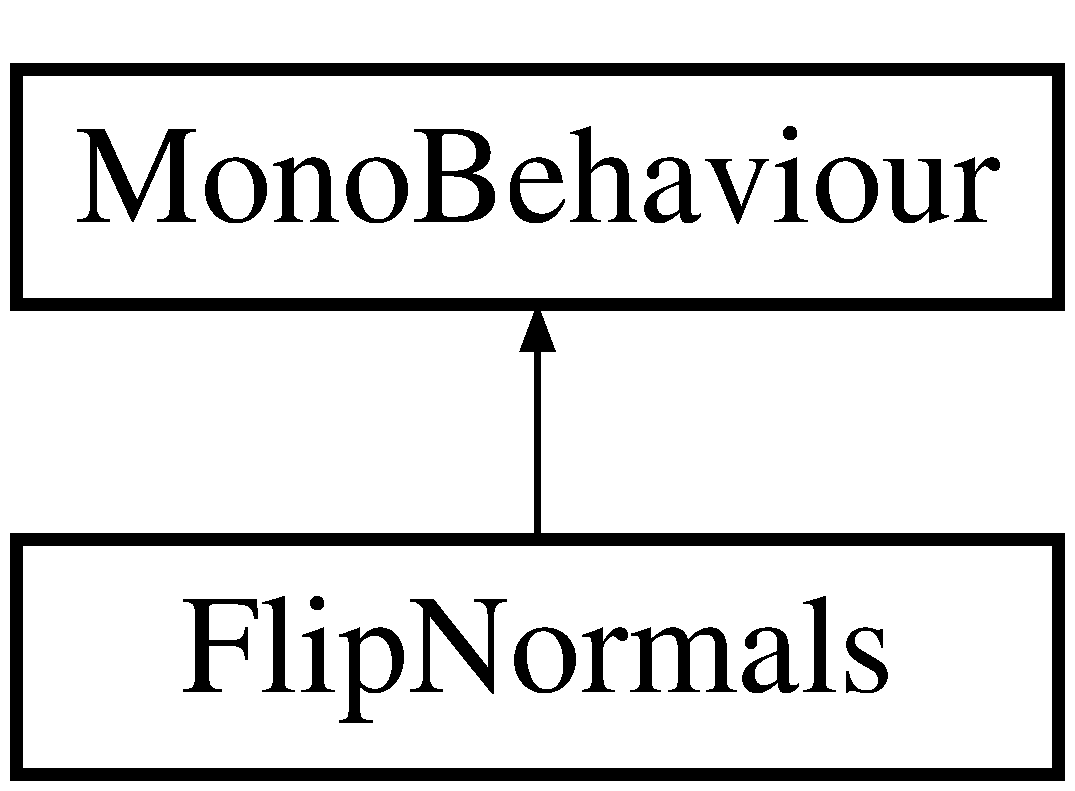
\includegraphics[height=2.000000cm]{class_flip_normals}
\end{center}
\end{figure}
\subsection*{Private Member Functions}
\begin{DoxyCompactItemize}
\item 
void \mbox{\hyperlink{class_flip_normals_ae09540466ec32870d991d67ec5424ec3}{Start}} ()
\end{DoxyCompactItemize}


\subsection{Detailed Description}
Use this to invert the normals of an object 



\subsection{Member Function Documentation}
\mbox{\Hypertarget{class_flip_normals_ae09540466ec32870d991d67ec5424ec3}\label{class_flip_normals_ae09540466ec32870d991d67ec5424ec3}} 
\index{Flip\+Normals@{Flip\+Normals}!Start@{Start}}
\index{Start@{Start}!Flip\+Normals@{Flip\+Normals}}
\subsubsection{\texorpdfstring{Start()}{Start()}}
{\footnotesize\ttfamily void Flip\+Normals.\+Start (\begin{DoxyParamCaption}{ }\end{DoxyParamCaption})\hspace{0.3cm}{\ttfamily [private]}}



The documentation for this class was generated from the following file\+:\begin{DoxyCompactItemize}
\item 
\mbox{\hyperlink{_flip_normals_8cs}{Flip\+Normals.\+cs}}\end{DoxyCompactItemize}

\hypertarget{class_force_field}{}\section{Force\+Field Class Reference}
\label{class_force_field}\index{Force\+Field@{Force\+Field}}


Class is used to destroy objects when they are thrown too far This is done by determining when the object exits the forcefield (On\+Trigger\+Exit) and when that happens it will be destroyed.  


Inheritance diagram for Force\+Field\+:\begin{figure}[H]
\begin{center}
\leavevmode
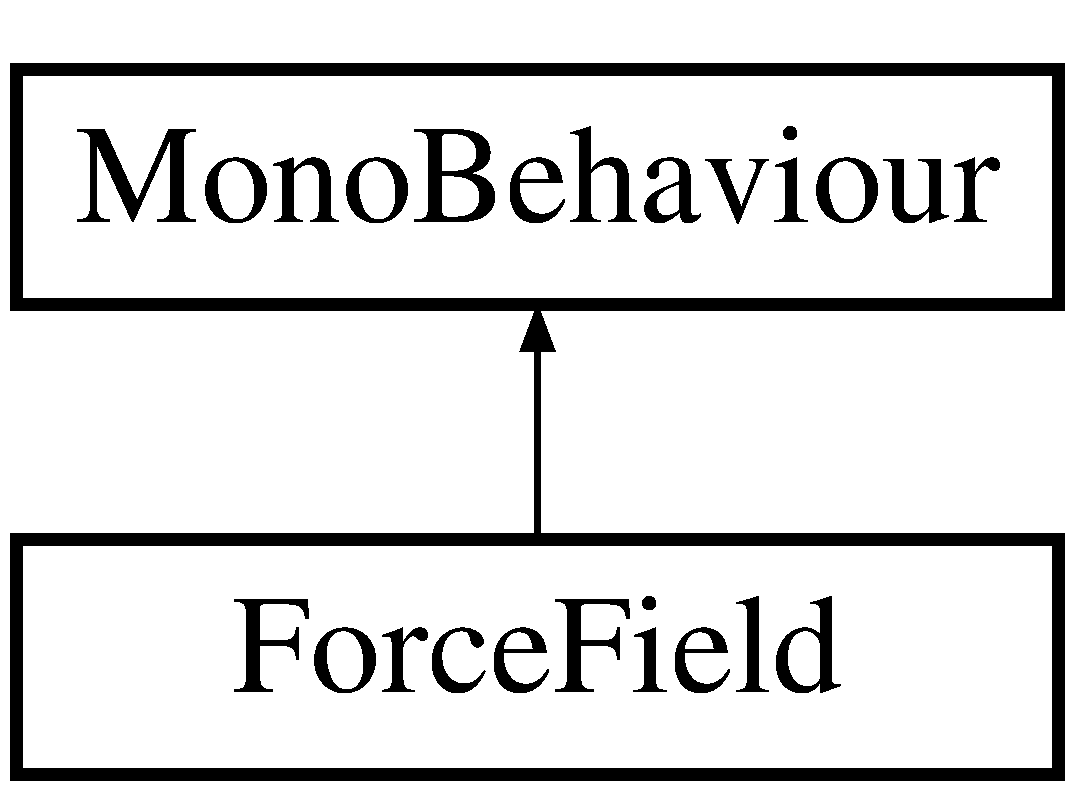
\includegraphics[height=2.000000cm]{class_force_field}
\end{center}
\end{figure}
\subsection*{Private Member Functions}
\begin{DoxyCompactItemize}
\item 
void \mbox{\hyperlink{class_force_field_a3a46258294cc671a8d35ebcc968602bb}{Update}} ()
\item 
void \mbox{\hyperlink{class_force_field_aa8354be76d0c19d705db2cc025e8095e}{On\+Trigger\+Enter}} (Collider other)
\item 
void \mbox{\hyperlink{class_force_field_a8ffe5c4cd5f6a4f2626f496760631c74}{On\+Trigger\+Exit}} (Collider other)
\end{DoxyCompactItemize}
\subsection*{Private Attributes}
\begin{DoxyCompactItemize}
\item 
Animator \mbox{\hyperlink{class_force_field_a48087ec1814d9b3b0c64d568c50704a8}{m\+\_\+\+Animator}}
\item 
bool \mbox{\hyperlink{class_force_field_add42e1b3ae6deec80beca3a10831bf71}{m\+\_\+\+In\+Trigger}}
\item 
Game\+Object \mbox{\hyperlink{class_force_field_a3fe0e589031437d56a08af4f313b9193}{m\+\_\+\+Ball}}
\end{DoxyCompactItemize}


\subsection{Detailed Description}
Class is used to destroy objects when they are thrown too far This is done by determining when the object exits the forcefield (On\+Trigger\+Exit) and when that happens it will be destroyed. 



\subsection{Member Function Documentation}
\mbox{\Hypertarget{class_force_field_aa8354be76d0c19d705db2cc025e8095e}\label{class_force_field_aa8354be76d0c19d705db2cc025e8095e}} 
\index{Force\+Field@{Force\+Field}!On\+Trigger\+Enter@{On\+Trigger\+Enter}}
\index{On\+Trigger\+Enter@{On\+Trigger\+Enter}!Force\+Field@{Force\+Field}}
\subsubsection{\texorpdfstring{On\+Trigger\+Enter()}{OnTriggerEnter()}}
{\footnotesize\ttfamily void Force\+Field.\+On\+Trigger\+Enter (\begin{DoxyParamCaption}\item[{Collider}]{other }\end{DoxyParamCaption})\hspace{0.3cm}{\ttfamily [private]}}

\mbox{\Hypertarget{class_force_field_a8ffe5c4cd5f6a4f2626f496760631c74}\label{class_force_field_a8ffe5c4cd5f6a4f2626f496760631c74}} 
\index{Force\+Field@{Force\+Field}!On\+Trigger\+Exit@{On\+Trigger\+Exit}}
\index{On\+Trigger\+Exit@{On\+Trigger\+Exit}!Force\+Field@{Force\+Field}}
\subsubsection{\texorpdfstring{On\+Trigger\+Exit()}{OnTriggerExit()}}
{\footnotesize\ttfamily void Force\+Field.\+On\+Trigger\+Exit (\begin{DoxyParamCaption}\item[{Collider}]{other }\end{DoxyParamCaption})\hspace{0.3cm}{\ttfamily [private]}}

\mbox{\Hypertarget{class_force_field_a3a46258294cc671a8d35ebcc968602bb}\label{class_force_field_a3a46258294cc671a8d35ebcc968602bb}} 
\index{Force\+Field@{Force\+Field}!Update@{Update}}
\index{Update@{Update}!Force\+Field@{Force\+Field}}
\subsubsection{\texorpdfstring{Update()}{Update()}}
{\footnotesize\ttfamily void Force\+Field.\+Update (\begin{DoxyParamCaption}{ }\end{DoxyParamCaption})\hspace{0.3cm}{\ttfamily [private]}}



\subsection{Member Data Documentation}
\mbox{\Hypertarget{class_force_field_a48087ec1814d9b3b0c64d568c50704a8}\label{class_force_field_a48087ec1814d9b3b0c64d568c50704a8}} 
\index{Force\+Field@{Force\+Field}!m\+\_\+\+Animator@{m\+\_\+\+Animator}}
\index{m\+\_\+\+Animator@{m\+\_\+\+Animator}!Force\+Field@{Force\+Field}}
\subsubsection{\texorpdfstring{m\+\_\+\+Animator}{m\_Animator}}
{\footnotesize\ttfamily Animator Force\+Field.\+m\+\_\+\+Animator\hspace{0.3cm}{\ttfamily [private]}}

\mbox{\Hypertarget{class_force_field_a3fe0e589031437d56a08af4f313b9193}\label{class_force_field_a3fe0e589031437d56a08af4f313b9193}} 
\index{Force\+Field@{Force\+Field}!m\+\_\+\+Ball@{m\+\_\+\+Ball}}
\index{m\+\_\+\+Ball@{m\+\_\+\+Ball}!Force\+Field@{Force\+Field}}
\subsubsection{\texorpdfstring{m\+\_\+\+Ball}{m\_Ball}}
{\footnotesize\ttfamily Game\+Object Force\+Field.\+m\+\_\+\+Ball\hspace{0.3cm}{\ttfamily [private]}}

\mbox{\Hypertarget{class_force_field_add42e1b3ae6deec80beca3a10831bf71}\label{class_force_field_add42e1b3ae6deec80beca3a10831bf71}} 
\index{Force\+Field@{Force\+Field}!m\+\_\+\+In\+Trigger@{m\+\_\+\+In\+Trigger}}
\index{m\+\_\+\+In\+Trigger@{m\+\_\+\+In\+Trigger}!Force\+Field@{Force\+Field}}
\subsubsection{\texorpdfstring{m\+\_\+\+In\+Trigger}{m\_InTrigger}}
{\footnotesize\ttfamily bool Force\+Field.\+m\+\_\+\+In\+Trigger\hspace{0.3cm}{\ttfamily [private]}}



The documentation for this class was generated from the following file\+:\begin{DoxyCompactItemize}
\item 
\mbox{\hyperlink{_force_field_8cs}{Force\+Field.\+cs}}\end{DoxyCompactItemize}

\hypertarget{class_intro_session_manager}{}\section{Intro\+Session\+Manager Class Reference}
\label{class_intro_session_manager}\index{Intro\+Session\+Manager@{Intro\+Session\+Manager}}
Inheritance diagram for Intro\+Session\+Manager\+:\begin{figure}[H]
\begin{center}
\leavevmode
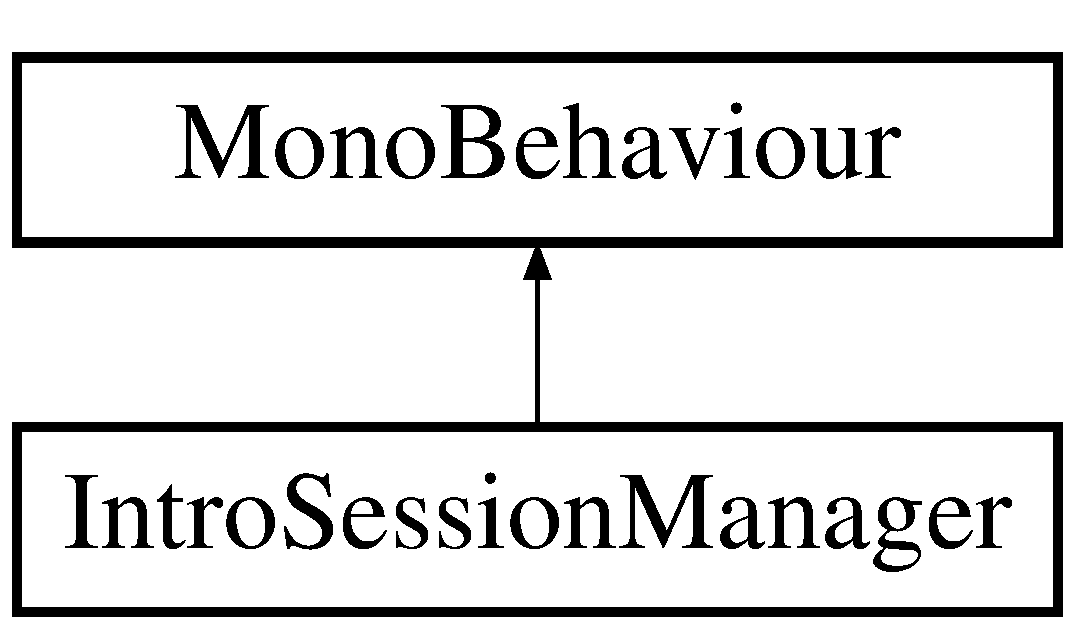
\includegraphics[height=2.000000cm]{class_intro_session_manager}
\end{center}
\end{figure}
\subsection*{Public Member Functions}
\begin{DoxyCompactItemize}
\item 
void \mbox{\hyperlink{class_intro_session_manager_a9541e181250bbfbfa2d16f62ccb64a22}{Move\+To\+Next\+Stage}} (float delay=0)
\begin{DoxyCompactList}\small\item\em Driver function to advance to the next scene with a specified delay \end{DoxyCompactList}\item 
void \mbox{\hyperlink{class_intro_session_manager_ab234b0587ea8c4283121ac8103ef67e1}{Spawn\+New\+Ball}} ()
\begin{DoxyCompactList}\small\item\em Spawns a new ball and destroys the old one if one exists \end{DoxyCompactList}\item 
void \mbox{\hyperlink{class_intro_session_manager_a0998c6878046777a1baecb46ff8859ec}{Open\+Button\+Box}} ()
\begin{DoxyCompactList}\small\item\em Method triggers the box to be opened \end{DoxyCompactList}\item 
void \mbox{\hyperlink{class_intro_session_manager_ac76f64b1d5b9e0a1a31b2f082708513b}{Close\+Button\+Box}} ()
\begin{DoxyCompactList}\small\item\em Method triggers the box to close \end{DoxyCompactList}\item 
void \mbox{\hyperlink{class_intro_session_manager_ab0c0444fb1525d86b4187c32cec0ce42}{Open\+Sliding\+Doors}} ()
\begin{DoxyCompactList}\small\item\em Method triggers opening the sliding doors \end{DoxyCompactList}\item 
void \mbox{\hyperlink{class_intro_session_manager_ad19be66a5259ad1075f5bec8389bb2ed}{Close\+Sliding\+Doors}} ()
\begin{DoxyCompactList}\small\item\em Method triggers closing the sliding doors \end{DoxyCompactList}\item 
void \mbox{\hyperlink{class_intro_session_manager_a7f844de6716bc367d539bd3a0dd835de}{Bring\+Box\+Into\+Scene}} ()
\begin{DoxyCompactList}\small\item\em Method triggers bringing the box into the scene \end{DoxyCompactList}\item 
void \mbox{\hyperlink{class_intro_session_manager_a238203538188c1c9407b816adae6487b}{Move\+Box\+Out\+Of\+Scene}} ()
\begin{DoxyCompactList}\small\item\em Method triggers bringing the box out of the scene \end{DoxyCompactList}\item 
void \mbox{\hyperlink{class_intro_session_manager_a158dbb9e63a362ad1f71380ad1f116db}{Toast}} (string msg, float length)
\begin{DoxyCompactList}\small\item\em Method displays a Toast on the Message\+Board \end{DoxyCompactList}\item 
void \mbox{\hyperlink{class_intro_session_manager_a6b31e91f5f7fb8d55555424b3f795750}{Move\+Robot\+To\+Position}} (Vector3 position, float speed=5f)
\begin{DoxyCompactList}\small\item\em Moves the robot to the Vector3 location passed in the param \end{DoxyCompactList}\item 
void \mbox{\hyperlink{class_intro_session_manager_a8e0deb467e6dbfcc9074221bfba81053}{Global\+Message}} (string msg)
\begin{DoxyCompactList}\small\item\em Displays a message to the user on the message board. \end{DoxyCompactList}\item 
void \mbox{\hyperlink{class_intro_session_manager_a97e1107140022bb06bfef6e4054ae69c}{Global\+Message}} (\mbox{\hyperlink{class_dialogue_element}{Dialogue\+Element}} ele)
\begin{DoxyCompactList}\small\item\em Driver function to display a message and audio from the {\ttfamily Dialog\+Element{\ttfamily  parameter. }}

{\ttfamily {\ttfamily  }}\end{DoxyCompactList}\item 
void \mbox{\hyperlink{class_intro_session_manager_af70a43fd234d1f362d0b9d75a613e9db}{Change\+Music}} (int track)
\item 
void \mbox{\hyperlink{class_intro_session_manager_a5f7f82cd17d0cfd8c54abd6dffcde081}{Highlight\+Button\+On}} (Game\+Object obj)
\item 
void \mbox{\hyperlink{class_intro_session_manager_afa85136787b9c937f76f92c22314341d}{Highlight\+Button\+Off}} (Game\+Object obj)
\begin{DoxyCompactList}\small\item\em Turns glow effect off of obj \end{DoxyCompactList}\item 
int \mbox{\hyperlink{class_intro_session_manager_a16f670a63e6d68ef3ae65573b3a7b01f}{Get\+Current\+Scene}} ()
\begin{DoxyCompactList}\small\item\em Returns the current scene. \end{DoxyCompactList}\item 
Game\+Object \mbox{\hyperlink{class_intro_session_manager_a7ce12de7f1dfcec0ad8b57f7e867a30d}{Get\+Home\+Button}} ()
\begin{DoxyCompactList}\small\item\em Returns a reference to the {\ttfamily home\+\_\+\+P\+LY} button. \end{DoxyCompactList}\item 
Game\+Object \mbox{\hyperlink{class_intro_session_manager_a78cade3f987f624f20d216b53a1c8f90}{Get\+Trigger\+Button}} ()
\begin{DoxyCompactList}\small\item\em Returns a reference to the {\ttfamily trigger\+\_\+\+P\+LY} button. \end{DoxyCompactList}\item 
Game\+Object \mbox{\hyperlink{class_intro_session_manager_a8932e2f5e73d5f9915a703f87e5c9f49}{Get\+Reticle}} ()
\begin{DoxyCompactList}\small\item\em Gets a reference to the reticle \end{DoxyCompactList}\item 
Game\+Object \mbox{\hyperlink{class_intro_session_manager_afbbc0627840abc6a3666eba25a7efd76}{Get\+Center\+Eye\+Anchor}} ()
\begin{DoxyCompactList}\small\item\em Returns a reference to the Center\+Eye\+Anchor (Camera the player is looking through) \end{DoxyCompactList}\item 
Game\+Object \mbox{\hyperlink{class_intro_session_manager_a836a60ce3ae8f1fb514c81f3c59da3ad}{Get\+Controller\+Model}} ()
\begin{DoxyCompactList}\small\item\em Returns a reference to the controller model \end{DoxyCompactList}\item 
Vector3 \mbox{\hyperlink{class_intro_session_manager_ab271ab8ae6b7e13929f05fd55670dc3f}{Get\+Robot\+Default\+Position}} ()
\begin{DoxyCompactList}\small\item\em Returns a reference to the default position of the robot in the scenes \end{DoxyCompactList}\item 
Image \mbox{\hyperlink{class_intro_session_manager_a918fbca0cbe7a7769c8a777e059f1375}{Get\+Loading\+Bar}} ()
\begin{DoxyCompactList}\small\item\em Returns a reference to the loading bar image \end{DoxyCompactList}\item 
void \mbox{\hyperlink{class_intro_session_manager_a2c3b7ee11852a65be6fb794c84de14f5}{Reticle\+Set\+Default\+State}} ()
\begin{DoxyCompactList}\small\item\em Function resets the state of the reticle to its default state. Pass in true to add a small delay before reverting to default. This could be used for when the user just clicks on an item instead of pressing and holding, so they have time to see the click was registered. \end{DoxyCompactList}\item 
void \mbox{\hyperlink{class_intro_session_manager_a31072153b257d37a5b1cd1566dd45d16}{Reticle\+Set\+Hover\+State}} ()
\begin{DoxyCompactList}\small\item\em Sets the reticle to its Hover state. Should be used when the user is hovering over an interactable item \end{DoxyCompactList}\item 
void \mbox{\hyperlink{class_intro_session_manager_aed37fcae779d3784743969ae0739c1c3}{Reticle\+Set\+Interacting}} ()
\item 
void \mbox{\hyperlink{class_intro_session_manager_a7ecdbb5df14f9c17bd6556467916f4aa}{Reticle\+Invalid\+Operation}} ()
\begin{DoxyCompactList}\small\item\em Driver method to start a coroutine that shows an invalid operation on the reticle (circle with line through it) \end{DoxyCompactList}\end{DoxyCompactItemize}
\subsection*{Static Public Attributes}
\begin{DoxyCompactItemize}
\item 
static readonly float \mbox{\hyperlink{class_intro_session_manager_a34742224aa0d8383b9153c24c4995e4c}{c\+\_\+\+T\+O\+A\+S\+T\+\_\+\+E\+X\+T\+RA}} = 6f
\item 
static readonly float \mbox{\hyperlink{class_intro_session_manager_ace53262c015b3c124166d5fcf5813b40}{c\+\_\+\+T\+O\+A\+S\+T\+\_\+\+L\+O\+NG}} = 4f
\item 
static readonly float \mbox{\hyperlink{class_intro_session_manager_af8478d0e7c13bd12f28b785b95a1851f}{c\+\_\+\+T\+O\+A\+S\+T\+\_\+\+S\+H\+O\+RT}} = 2f
\item 
static readonly Color \mbox{\hyperlink{class_intro_session_manager_aba87a1dd94fe94906cc2b8590d4bc430}{c\+\_\+\+C\+O\+L\+O\+R\+\_\+\+L\+I\+G\+H\+T\+G\+R\+AY}} = new Color(.\+8f, .\+8f, .\+8f, 1f)
\item 
static \mbox{\hyperlink{class_intro_session_manager}{Intro\+Session\+Manager}} \mbox{\hyperlink{class_intro_session_manager_a206bd6bc9edad9b90ee89aa85b00000c}{s\+\_\+\+Instance}} = null
\item 
static \mbox{\hyperlink{class_v_r_standard_assets_1_1_utils_1_1_raycaster_v_r}{Raycaster\+VR}} \mbox{\hyperlink{class_intro_session_manager_ae797af3e2ada3170f3c9f533b88a3806}{s\+\_\+\+Raycaster\+Script}}
\end{DoxyCompactItemize}
\subsection*{Private Member Functions}
\begin{DoxyCompactItemize}
\item 
void \mbox{\hyperlink{class_intro_session_manager_a7c36bee635e59c09531ed8c64665b0fd}{Awake}} ()
\item 
void \mbox{\hyperlink{class_intro_session_manager_af44cc6aa8fff0329411659f44ba29475}{Start}} ()
\item 
void \mbox{\hyperlink{class_intro_session_manager_ad430deae2d91891de87162529e915ab9}{Update}} ()
\item 
I\+Enumerator \mbox{\hyperlink{class_intro_session_manager_abbbe032dd983857f6a0d843686738bfc}{Tutorial\+Introduction}} ()
\begin{DoxyCompactList}\small\item\em Begins the introduction to the tutorial \end{DoxyCompactList}\item 
I\+Enumerator \mbox{\hyperlink{class_intro_session_manager_a93c526ae0e6c546c2ee76a6d150b4781}{Advance\+Stage}} (float delay)
\begin{DoxyCompactList}\small\item\em Method is used as a coroutine to advance through the stage \end{DoxyCompactList}\item 
void \mbox{\hyperlink{class_intro_session_manager_a6731f9f957d00bf47bb55f745f3af95b}{Opening\+Sliding\+Doors}} ()
\begin{DoxyCompactList}\small\item\em Method gets called in update. Opens the sliding doors one step per call. \end{DoxyCompactList}\item 
void \mbox{\hyperlink{class_intro_session_manager_a7cc8cfc2810a691bbc149f9688f68118}{Closing\+Sliding\+Doors}} ()
\begin{DoxyCompactList}\small\item\em Method gets called in update. Closes the sliding doors one step per call. \end{DoxyCompactList}\item 
I\+Enumerator \mbox{\hyperlink{class_intro_session_manager_ad809a83bf76ede581699a9efd0280a4c}{Show\+Toast\+Length}} (string msg, float length)
\begin{DoxyCompactList}\small\item\em Shows a Toast message on the Message Board for a duration of time. \end{DoxyCompactList}\item 
I\+Enumerator \mbox{\hyperlink{class_intro_session_manager_a1f4d274eb1210032091a14668007010e}{Intro\+In}} ()
\item 
void \mbox{\hyperlink{class_intro_session_manager_a96f4ea7bcbd9459bf04ccc1663cc7259}{Intro\+Out}} ()
\begin{DoxyCompactList}\small\item\em Controls the flow of the tutorial introduction \end{DoxyCompactList}\item 
void \mbox{\hyperlink{class_intro_session_manager_a8ea998890634808b09e0f05a68d81d64}{Do\+Bring\+Box\+Into\+Scene}} ()
\begin{DoxyCompactList}\small\item\em Moves the box into the scene \end{DoxyCompactList}\item 
void \mbox{\hyperlink{class_intro_session_manager_a1458287c5067948bca87eaeb05dc9ebf}{Do\+Move\+Box\+Out\+Of\+Scene}} ()
\begin{DoxyCompactList}\small\item\em Move the box out of the scene \end{DoxyCompactList}\item 
void \mbox{\hyperlink{class_intro_session_manager_ae9859df135187ffdfccd320d8d011500}{Opening\+Button\+Box}} ()
\begin{DoxyCompactList}\small\item\em Opens the doors on the box and brings the button out of the box \end{DoxyCompactList}\item 
void \mbox{\hyperlink{class_intro_session_manager_a58ae098b28554a98916370ad0647fd87}{Closing\+Button\+Box}} ()
\begin{DoxyCompactList}\small\item\em Method closes the doors on the button box \end{DoxyCompactList}\item 
I\+Enumerator \mbox{\hyperlink{class_intro_session_manager_ad0caff53bd4a5a65499e13c4a2f20212}{Do\+Invalid\+Operation}} ()
\begin{DoxyCompactList}\small\item\em Displays the invalid operation image on the reticle for 1 second \end{DoxyCompactList}\end{DoxyCompactItemize}
\subsection*{Private Attributes}
\begin{DoxyCompactItemize}
\item 
readonly float \mbox{\hyperlink{class_intro_session_manager_ae24a9c30326fa7bff220c8a88c97cbbd}{c\+\_\+\+Door\+Forward\+Speed}} = 0.\+1f
\item 
readonly float \mbox{\hyperlink{class_intro_session_manager_a2704a73e12814b6c83f5daec3e962723}{c\+\_\+\+Door\+Side\+Speed}} = 0.\+8f
\item 
\mbox{\hyperlink{class_dialogue}{Dialogue}} \mbox{\hyperlink{class_intro_session_manager_ab695398be29615d5e14df3d1e0019059}{m\+\_\+\+Dialogue\+Instructions}}
\item 
\mbox{\hyperlink{class_dialogue}{Dialogue}} \mbox{\hyperlink{class_intro_session_manager_a470ec4b3778051a627d6c24f40fc61d3}{music\+Clips}}
\item 
Game\+Object \mbox{\hyperlink{class_intro_session_manager_a4acb0cd1ca734c4b2d287c21e0d94f66}{m\+\_\+\+Reticle}}
\item 
Game\+Object \mbox{\hyperlink{class_intro_session_manager_a99b3acd5b53deddb2707d0a572524b2d}{m\+\_\+\+Robot}}
\item 
Game\+Object \mbox{\hyperlink{class_intro_session_manager_a235a181ca063d1fda1e971e7f52d0ebc}{m\+\_\+\+Center\+Eye\+Anchor}}
\item 
Game\+Object \mbox{\hyperlink{class_intro_session_manager_a24b3a594b1749a687454f4f580452d7a}{m\+\_\+\+Ball\+Prefab}}
\item 
Game\+Object \mbox{\hyperlink{class_intro_session_manager_a29cd7383da1ce27357209f218bb4bdb6}{m\+\_\+\+Controller\+Model}}
\item 
Game\+Object \mbox{\hyperlink{class_intro_session_manager_aca0fa30bffd1159e786232541b0f254a}{m\+\_\+\+Starting\+Platform}}
\item 
Game\+Object \mbox{\hyperlink{class_intro_session_manager_a86f65280712498492706c8c460c2ecef}{m\+\_\+\+Sliding\+Door\+Right}}
\item 
Game\+Object \mbox{\hyperlink{class_intro_session_manager_a8f507b5c62504d8f0b3c99583080d1c6}{m\+\_\+\+Sliding\+Door\+Left}}
\item 
Game\+Object \mbox{\hyperlink{class_intro_session_manager_a1ec45e159d4b876b370443534a4140ee}{m\+\_\+\+Home\+Button}}
\item 
Game\+Object \mbox{\hyperlink{class_intro_session_manager_a4ce2d50d7ff83169dc8224b199ac7e68}{m\+\_\+\+Trigger\+Button}}
\item 
Game\+Object \mbox{\hyperlink{class_intro_session_manager_ab9bab6c380a3dcc60825a13fffd65414}{m\+\_\+\+Button\+Box}}
\item 
Game\+Object \mbox{\hyperlink{class_intro_session_manager_ac1ebde5d641b0fbe3f5c7d5f466406c4}{m\+\_\+\+Left\+Door\+Button\+Box}}
\item 
Game\+Object \mbox{\hyperlink{class_intro_session_manager_a156fbcdf5bd354b60a3a864e63149d74}{m\+\_\+\+Right\+Door\+Button\+Box}}
\item 
Game\+Object \mbox{\hyperlink{class_intro_session_manager_af373a8e1add9dccca5985f10db4c3c13}{m\+\_\+\+Button}}
\item 
Game\+Object \mbox{\hyperlink{class_intro_session_manager_ac7c8eb1a21d3cf81c759c6088e02fac5}{m\+\_\+\+Platform\+Raised\+Position}}
\item 
Game\+Object \mbox{\hyperlink{class_intro_session_manager_a0c8ac69af055d55bef22944606a0232d}{m\+\_\+\+Robot\+Intro\+Dest1}}
\item 
Game\+Object \mbox{\hyperlink{class_intro_session_manager_ab609b1106ef0b8526612fc511bf711f3}{m\+\_\+\+Robot\+Default\+Position}}
\item 
Game\+Object \mbox{\hyperlink{class_intro_session_manager_a0de05def8a32179bbea80d1d4a296829}{m\+\_\+\+Message\+Panel}}
\item 
Game\+Object \mbox{\hyperlink{class_intro_session_manager_a1a92991967b5d8f322610a85a548d4df}{m\+\_\+\+Message\+Board\+Border}}
\item 
Material \mbox{\hyperlink{class_intro_session_manager_a74a01ae10424770fa43f60f407cf2cf1}{m\+\_\+\+Highlight\+Material}}
\item 
Audio\+Source \mbox{\hyperlink{class_intro_session_manager_a184d9e4647fb9b54d6292971c0d36590}{m\+\_\+\+Robot\+Audio\+Source}}
\item 
Audio\+Source \mbox{\hyperlink{class_intro_session_manager_af435af1ecc0838851211ff54a82c750b}{m\+\_\+\+Stage\+Music}}
\item 
Text \mbox{\hyperlink{class_intro_session_manager_ace9b36a18f2d4f140836a98827011cef}{m\+\_\+\+Global\+Message\+Board\+Text}}
\item 
Text \mbox{\hyperlink{class_intro_session_manager_affe78d60003972c8f0dc9e9e1e63e50e}{m\+\_\+\+Clock\+Text}}
\item 
bool \mbox{\hyperlink{class_intro_session_manager_a4f6bbbe92b466fc9713ea809e44b8715}{m\+\_\+\+Test\+Mode}}
\item 
int \mbox{\hyperlink{class_intro_session_manager_aaeefdeac17668edbd7638eea2c771c5f}{m\+\_\+\+Start\+Scene}}
\item 
Image \mbox{\hyperlink{class_intro_session_manager_aa6a3bae892b3055d81deec38c303f37c}{m\+\_\+\+Invalid\+Operation\+Image}}
\item 
Image \mbox{\hyperlink{class_intro_session_manager_a3a614c679e3c032bbd9b9a12e525ef68}{m\+\_\+\+Reticle\+Outer\+Circle}}
\item 
Image \mbox{\hyperlink{class_intro_session_manager_ae70b15e66a1828fac715707eb92d8f70}{m\+\_\+\+Reticle\+Inner\+Circle}}
\item 
Image \mbox{\hyperlink{class_intro_session_manager_a3ab9cd9a1ca04c1570a3e4d35a382f80}{m\+\_\+\+Loading\+Bar}}
\item 
int \mbox{\hyperlink{class_intro_session_manager_aed8065a46f21ce1d465d0523b9cd6a94}{i\+\_\+\+Current\+Scene}} = 0
\item 
Animator \mbox{\hyperlink{class_intro_session_manager_aba1ae4db2632c630034c828a55ff44a8}{m\+\_\+\+Robot\+Animator}}
\item 
string \mbox{[}$\,$\mbox{]} \mbox{\hyperlink{class_intro_session_manager_a4e9865d9b05cc6f052cea4bd7d9b7e1f}{m\+\_\+\+Scenes}}
\item 
bool \mbox{\hyperlink{class_intro_session_manager_aca63a7e6cd979f5110c3054024284fa4}{m\+\_\+\+Opening\+Sliding\+Doors}}
\item 
bool \mbox{\hyperlink{class_intro_session_manager_ab296c21bb7534168337854df487ecd6a}{m\+\_\+\+Closing\+Sliding\+Doors}}
\item 
bool \mbox{\hyperlink{class_intro_session_manager_a30e27176dbb3a3eb25c429ad65a88200}{m\+\_\+\+Intro\+In}}
\item 
bool \mbox{\hyperlink{class_intro_session_manager_a5896398e369471a9085d7208309cc730}{m\+\_\+\+Intro\+Out}}
\item 
bool \mbox{\hyperlink{class_intro_session_manager_ada16df52e05f0c7780efdb0f14b0509e}{m\+\_\+\+Opening\+Box}}
\item 
bool \mbox{\hyperlink{class_intro_session_manager_ab238042bfbf997400f5abce96cc0408f}{m\+\_\+\+Closing\+Box}}
\item 
bool \mbox{\hyperlink{class_intro_session_manager_abce70a4bbbb5858a2b7a08b4305809a0}{m\+\_\+\+Bring\+Box\+Into\+Scene}}
\item 
bool \mbox{\hyperlink{class_intro_session_manager_a16bbfff4e9b4adb0f3372357d222ee5f}{m\+\_\+\+Move\+Box\+Out\+Of\+Scene}}
\item 
Vector3 \mbox{\hyperlink{class_intro_session_manager_a94c3ed99ca9e372cd778c89403a5888a}{m\+\_\+\+Platform\+Start\+Pos}}
\item 
Game\+Object \mbox{\hyperlink{class_intro_session_manager_aba1a41efd4328b389c8dd6a301b20a4a}{m\+\_\+\+Ball\+Clone}}
\item 
bool \mbox{\hyperlink{class_intro_session_manager_ade25d99d3058a14d4c2738a51281780e}{m\+\_\+\+Showing\+Toast}}
\item 
Hashtable \mbox{\hyperlink{class_intro_session_manager_ad719cd26d73b589cc92fdb3b4ad9a996}{m\+\_\+\+Material\+Map}}
\item 
I\+Enumerator \mbox{\hyperlink{class_intro_session_manager_ac3a4cf5ad448811271447cf9fa4b6d2b}{m\+\_\+\+Invalid\+Operation\+Coroutine}}
\item 
I\+Enumerator \mbox{\hyperlink{class_intro_session_manager_a709ed8345dde73d0a36c3c59e03f18f5}{m\+\_\+\+Toast\+Coroutine}} = null
\item 
I\+Enumerator \mbox{\hyperlink{class_intro_session_manager_acedcbccfb11e49f5279cbc11e7832c67}{m\+\_\+\+Reticle\+State\+Coroutine}}
\item 
string \mbox{\hyperlink{class_intro_session_manager_ab430fe3c2e7472725e639ba1dbe22822}{m\+\_\+\+Prev\+Message}}
\item 
Color \mbox{\hyperlink{class_intro_session_manager_a439437ada3c600dbffb75b971aafc45a}{m\+\_\+\+Prev\+Color}}
\end{DoxyCompactItemize}


\subsection{Member Function Documentation}
\mbox{\Hypertarget{class_intro_session_manager_a93c526ae0e6c546c2ee76a6d150b4781}\label{class_intro_session_manager_a93c526ae0e6c546c2ee76a6d150b4781}} 
\index{Intro\+Session\+Manager@{Intro\+Session\+Manager}!Advance\+Stage@{Advance\+Stage}}
\index{Advance\+Stage@{Advance\+Stage}!Intro\+Session\+Manager@{Intro\+Session\+Manager}}
\subsubsection{\texorpdfstring{Advance\+Stage()}{AdvanceStage()}}
{\footnotesize\ttfamily I\+Enumerator Intro\+Session\+Manager.\+Advance\+Stage (\begin{DoxyParamCaption}\item[{float}]{delay }\end{DoxyParamCaption})\hspace{0.3cm}{\ttfamily [private]}}



Method is used as a coroutine to advance through the stage 


\begin{DoxyParams}{Parameters}
{\em delay} & The time delay between scene trasitions\\
\hline
\end{DoxyParams}
\begin{DoxyReturn}{Returns}
An I\+Enumerator that can reference this specific coroutine
\end{DoxyReturn}
\mbox{\Hypertarget{class_intro_session_manager_a7c36bee635e59c09531ed8c64665b0fd}\label{class_intro_session_manager_a7c36bee635e59c09531ed8c64665b0fd}} 
\index{Intro\+Session\+Manager@{Intro\+Session\+Manager}!Awake@{Awake}}
\index{Awake@{Awake}!Intro\+Session\+Manager@{Intro\+Session\+Manager}}
\subsubsection{\texorpdfstring{Awake()}{Awake()}}
{\footnotesize\ttfamily void Intro\+Session\+Manager.\+Awake (\begin{DoxyParamCaption}{ }\end{DoxyParamCaption})\hspace{0.3cm}{\ttfamily [private]}}

\mbox{\Hypertarget{class_intro_session_manager_a7f844de6716bc367d539bd3a0dd835de}\label{class_intro_session_manager_a7f844de6716bc367d539bd3a0dd835de}} 
\index{Intro\+Session\+Manager@{Intro\+Session\+Manager}!Bring\+Box\+Into\+Scene@{Bring\+Box\+Into\+Scene}}
\index{Bring\+Box\+Into\+Scene@{Bring\+Box\+Into\+Scene}!Intro\+Session\+Manager@{Intro\+Session\+Manager}}
\subsubsection{\texorpdfstring{Bring\+Box\+Into\+Scene()}{BringBoxIntoScene()}}
{\footnotesize\ttfamily void Intro\+Session\+Manager.\+Bring\+Box\+Into\+Scene (\begin{DoxyParamCaption}{ }\end{DoxyParamCaption})}



Method triggers bringing the box into the scene 

\mbox{\Hypertarget{class_intro_session_manager_af70a43fd234d1f362d0b9d75a613e9db}\label{class_intro_session_manager_af70a43fd234d1f362d0b9d75a613e9db}} 
\index{Intro\+Session\+Manager@{Intro\+Session\+Manager}!Change\+Music@{Change\+Music}}
\index{Change\+Music@{Change\+Music}!Intro\+Session\+Manager@{Intro\+Session\+Manager}}
\subsubsection{\texorpdfstring{Change\+Music()}{ChangeMusic()}}
{\footnotesize\ttfamily void Intro\+Session\+Manager.\+Change\+Music (\begin{DoxyParamCaption}\item[{int}]{track }\end{DoxyParamCaption})}

\mbox{\Hypertarget{class_intro_session_manager_ac76f64b1d5b9e0a1a31b2f082708513b}\label{class_intro_session_manager_ac76f64b1d5b9e0a1a31b2f082708513b}} 
\index{Intro\+Session\+Manager@{Intro\+Session\+Manager}!Close\+Button\+Box@{Close\+Button\+Box}}
\index{Close\+Button\+Box@{Close\+Button\+Box}!Intro\+Session\+Manager@{Intro\+Session\+Manager}}
\subsubsection{\texorpdfstring{Close\+Button\+Box()}{CloseButtonBox()}}
{\footnotesize\ttfamily void Intro\+Session\+Manager.\+Close\+Button\+Box (\begin{DoxyParamCaption}{ }\end{DoxyParamCaption})}



Method triggers the box to close 

\mbox{\Hypertarget{class_intro_session_manager_ad19be66a5259ad1075f5bec8389bb2ed}\label{class_intro_session_manager_ad19be66a5259ad1075f5bec8389bb2ed}} 
\index{Intro\+Session\+Manager@{Intro\+Session\+Manager}!Close\+Sliding\+Doors@{Close\+Sliding\+Doors}}
\index{Close\+Sliding\+Doors@{Close\+Sliding\+Doors}!Intro\+Session\+Manager@{Intro\+Session\+Manager}}
\subsubsection{\texorpdfstring{Close\+Sliding\+Doors()}{CloseSlidingDoors()}}
{\footnotesize\ttfamily void Intro\+Session\+Manager.\+Close\+Sliding\+Doors (\begin{DoxyParamCaption}{ }\end{DoxyParamCaption})}



Method triggers closing the sliding doors 

\mbox{\Hypertarget{class_intro_session_manager_a58ae098b28554a98916370ad0647fd87}\label{class_intro_session_manager_a58ae098b28554a98916370ad0647fd87}} 
\index{Intro\+Session\+Manager@{Intro\+Session\+Manager}!Closing\+Button\+Box@{Closing\+Button\+Box}}
\index{Closing\+Button\+Box@{Closing\+Button\+Box}!Intro\+Session\+Manager@{Intro\+Session\+Manager}}
\subsubsection{\texorpdfstring{Closing\+Button\+Box()}{ClosingButtonBox()}}
{\footnotesize\ttfamily void Intro\+Session\+Manager.\+Closing\+Button\+Box (\begin{DoxyParamCaption}{ }\end{DoxyParamCaption})\hspace{0.3cm}{\ttfamily [private]}}



Method closes the doors on the button box 

\mbox{\Hypertarget{class_intro_session_manager_a7cc8cfc2810a691bbc149f9688f68118}\label{class_intro_session_manager_a7cc8cfc2810a691bbc149f9688f68118}} 
\index{Intro\+Session\+Manager@{Intro\+Session\+Manager}!Closing\+Sliding\+Doors@{Closing\+Sliding\+Doors}}
\index{Closing\+Sliding\+Doors@{Closing\+Sliding\+Doors}!Intro\+Session\+Manager@{Intro\+Session\+Manager}}
\subsubsection{\texorpdfstring{Closing\+Sliding\+Doors()}{ClosingSlidingDoors()}}
{\footnotesize\ttfamily void Intro\+Session\+Manager.\+Closing\+Sliding\+Doors (\begin{DoxyParamCaption}{ }\end{DoxyParamCaption})\hspace{0.3cm}{\ttfamily [private]}}



Method gets called in update. Closes the sliding doors one step per call. 

\mbox{\Hypertarget{class_intro_session_manager_a8ea998890634808b09e0f05a68d81d64}\label{class_intro_session_manager_a8ea998890634808b09e0f05a68d81d64}} 
\index{Intro\+Session\+Manager@{Intro\+Session\+Manager}!Do\+Bring\+Box\+Into\+Scene@{Do\+Bring\+Box\+Into\+Scene}}
\index{Do\+Bring\+Box\+Into\+Scene@{Do\+Bring\+Box\+Into\+Scene}!Intro\+Session\+Manager@{Intro\+Session\+Manager}}
\subsubsection{\texorpdfstring{Do\+Bring\+Box\+Into\+Scene()}{DoBringBoxIntoScene()}}
{\footnotesize\ttfamily void Intro\+Session\+Manager.\+Do\+Bring\+Box\+Into\+Scene (\begin{DoxyParamCaption}{ }\end{DoxyParamCaption})\hspace{0.3cm}{\ttfamily [private]}}



Moves the box into the scene 

\mbox{\Hypertarget{class_intro_session_manager_ad0caff53bd4a5a65499e13c4a2f20212}\label{class_intro_session_manager_ad0caff53bd4a5a65499e13c4a2f20212}} 
\index{Intro\+Session\+Manager@{Intro\+Session\+Manager}!Do\+Invalid\+Operation@{Do\+Invalid\+Operation}}
\index{Do\+Invalid\+Operation@{Do\+Invalid\+Operation}!Intro\+Session\+Manager@{Intro\+Session\+Manager}}
\subsubsection{\texorpdfstring{Do\+Invalid\+Operation()}{DoInvalidOperation()}}
{\footnotesize\ttfamily I\+Enumerator Intro\+Session\+Manager.\+Do\+Invalid\+Operation (\begin{DoxyParamCaption}{ }\end{DoxyParamCaption})\hspace{0.3cm}{\ttfamily [private]}}



Displays the invalid operation image on the reticle for 1 second 

\begin{DoxyReturn}{Returns}
A reference to the coroutine
\end{DoxyReturn}
\mbox{\Hypertarget{class_intro_session_manager_a1458287c5067948bca87eaeb05dc9ebf}\label{class_intro_session_manager_a1458287c5067948bca87eaeb05dc9ebf}} 
\index{Intro\+Session\+Manager@{Intro\+Session\+Manager}!Do\+Move\+Box\+Out\+Of\+Scene@{Do\+Move\+Box\+Out\+Of\+Scene}}
\index{Do\+Move\+Box\+Out\+Of\+Scene@{Do\+Move\+Box\+Out\+Of\+Scene}!Intro\+Session\+Manager@{Intro\+Session\+Manager}}
\subsubsection{\texorpdfstring{Do\+Move\+Box\+Out\+Of\+Scene()}{DoMoveBoxOutOfScene()}}
{\footnotesize\ttfamily void Intro\+Session\+Manager.\+Do\+Move\+Box\+Out\+Of\+Scene (\begin{DoxyParamCaption}{ }\end{DoxyParamCaption})\hspace{0.3cm}{\ttfamily [private]}}



Move the box out of the scene 

\mbox{\Hypertarget{class_intro_session_manager_afbbc0627840abc6a3666eba25a7efd76}\label{class_intro_session_manager_afbbc0627840abc6a3666eba25a7efd76}} 
\index{Intro\+Session\+Manager@{Intro\+Session\+Manager}!Get\+Center\+Eye\+Anchor@{Get\+Center\+Eye\+Anchor}}
\index{Get\+Center\+Eye\+Anchor@{Get\+Center\+Eye\+Anchor}!Intro\+Session\+Manager@{Intro\+Session\+Manager}}
\subsubsection{\texorpdfstring{Get\+Center\+Eye\+Anchor()}{GetCenterEyeAnchor()}}
{\footnotesize\ttfamily Game\+Object Intro\+Session\+Manager.\+Get\+Center\+Eye\+Anchor (\begin{DoxyParamCaption}{ }\end{DoxyParamCaption})}



Returns a reference to the Center\+Eye\+Anchor (Camera the player is looking through) 

\begin{DoxyReturn}{Returns}
A reference to the Center\+Eye\+Anchor
\end{DoxyReturn}
\mbox{\Hypertarget{class_intro_session_manager_a836a60ce3ae8f1fb514c81f3c59da3ad}\label{class_intro_session_manager_a836a60ce3ae8f1fb514c81f3c59da3ad}} 
\index{Intro\+Session\+Manager@{Intro\+Session\+Manager}!Get\+Controller\+Model@{Get\+Controller\+Model}}
\index{Get\+Controller\+Model@{Get\+Controller\+Model}!Intro\+Session\+Manager@{Intro\+Session\+Manager}}
\subsubsection{\texorpdfstring{Get\+Controller\+Model()}{GetControllerModel()}}
{\footnotesize\ttfamily Game\+Object Intro\+Session\+Manager.\+Get\+Controller\+Model (\begin{DoxyParamCaption}{ }\end{DoxyParamCaption})}



Returns a reference to the controller model 

\begin{DoxyReturn}{Returns}
A reference to the controller model
\end{DoxyReturn}
\mbox{\Hypertarget{class_intro_session_manager_a16f670a63e6d68ef3ae65573b3a7b01f}\label{class_intro_session_manager_a16f670a63e6d68ef3ae65573b3a7b01f}} 
\index{Intro\+Session\+Manager@{Intro\+Session\+Manager}!Get\+Current\+Scene@{Get\+Current\+Scene}}
\index{Get\+Current\+Scene@{Get\+Current\+Scene}!Intro\+Session\+Manager@{Intro\+Session\+Manager}}
\subsubsection{\texorpdfstring{Get\+Current\+Scene()}{GetCurrentScene()}}
{\footnotesize\ttfamily int Intro\+Session\+Manager.\+Get\+Current\+Scene (\begin{DoxyParamCaption}{ }\end{DoxyParamCaption})}



Returns the current scene. 

\begin{DoxyReturn}{Returns}
The current scene.
\end{DoxyReturn}
\mbox{\Hypertarget{class_intro_session_manager_a7ce12de7f1dfcec0ad8b57f7e867a30d}\label{class_intro_session_manager_a7ce12de7f1dfcec0ad8b57f7e867a30d}} 
\index{Intro\+Session\+Manager@{Intro\+Session\+Manager}!Get\+Home\+Button@{Get\+Home\+Button}}
\index{Get\+Home\+Button@{Get\+Home\+Button}!Intro\+Session\+Manager@{Intro\+Session\+Manager}}
\subsubsection{\texorpdfstring{Get\+Home\+Button()}{GetHomeButton()}}
{\footnotesize\ttfamily Game\+Object Intro\+Session\+Manager.\+Get\+Home\+Button (\begin{DoxyParamCaption}{ }\end{DoxyParamCaption})}



Returns a reference to the {\ttfamily home\+\_\+\+P\+LY} button. 

\begin{DoxyReturn}{Returns}
The home button
\end{DoxyReturn}
\mbox{\Hypertarget{class_intro_session_manager_a918fbca0cbe7a7769c8a777e059f1375}\label{class_intro_session_manager_a918fbca0cbe7a7769c8a777e059f1375}} 
\index{Intro\+Session\+Manager@{Intro\+Session\+Manager}!Get\+Loading\+Bar@{Get\+Loading\+Bar}}
\index{Get\+Loading\+Bar@{Get\+Loading\+Bar}!Intro\+Session\+Manager@{Intro\+Session\+Manager}}
\subsubsection{\texorpdfstring{Get\+Loading\+Bar()}{GetLoadingBar()}}
{\footnotesize\ttfamily Image Intro\+Session\+Manager.\+Get\+Loading\+Bar (\begin{DoxyParamCaption}{ }\end{DoxyParamCaption})}



Returns a reference to the loading bar image 

\begin{DoxyReturn}{Returns}
A reference to the loading bar image
\end{DoxyReturn}
\mbox{\Hypertarget{class_intro_session_manager_a8932e2f5e73d5f9915a703f87e5c9f49}\label{class_intro_session_manager_a8932e2f5e73d5f9915a703f87e5c9f49}} 
\index{Intro\+Session\+Manager@{Intro\+Session\+Manager}!Get\+Reticle@{Get\+Reticle}}
\index{Get\+Reticle@{Get\+Reticle}!Intro\+Session\+Manager@{Intro\+Session\+Manager}}
\subsubsection{\texorpdfstring{Get\+Reticle()}{GetReticle()}}
{\footnotesize\ttfamily Game\+Object Intro\+Session\+Manager.\+Get\+Reticle (\begin{DoxyParamCaption}{ }\end{DoxyParamCaption})}



Gets a reference to the reticle 

\begin{DoxyReturn}{Returns}
The Reticle
\end{DoxyReturn}
\mbox{\Hypertarget{class_intro_session_manager_ab271ab8ae6b7e13929f05fd55670dc3f}\label{class_intro_session_manager_ab271ab8ae6b7e13929f05fd55670dc3f}} 
\index{Intro\+Session\+Manager@{Intro\+Session\+Manager}!Get\+Robot\+Default\+Position@{Get\+Robot\+Default\+Position}}
\index{Get\+Robot\+Default\+Position@{Get\+Robot\+Default\+Position}!Intro\+Session\+Manager@{Intro\+Session\+Manager}}
\subsubsection{\texorpdfstring{Get\+Robot\+Default\+Position()}{GetRobotDefaultPosition()}}
{\footnotesize\ttfamily Vector3 Intro\+Session\+Manager.\+Get\+Robot\+Default\+Position (\begin{DoxyParamCaption}{ }\end{DoxyParamCaption})}



Returns a reference to the default position of the robot in the scenes 

\begin{DoxyReturn}{Returns}
A reference to the default position of the robot in the scenes
\end{DoxyReturn}
\mbox{\Hypertarget{class_intro_session_manager_a78cade3f987f624f20d216b53a1c8f90}\label{class_intro_session_manager_a78cade3f987f624f20d216b53a1c8f90}} 
\index{Intro\+Session\+Manager@{Intro\+Session\+Manager}!Get\+Trigger\+Button@{Get\+Trigger\+Button}}
\index{Get\+Trigger\+Button@{Get\+Trigger\+Button}!Intro\+Session\+Manager@{Intro\+Session\+Manager}}
\subsubsection{\texorpdfstring{Get\+Trigger\+Button()}{GetTriggerButton()}}
{\footnotesize\ttfamily Game\+Object Intro\+Session\+Manager.\+Get\+Trigger\+Button (\begin{DoxyParamCaption}{ }\end{DoxyParamCaption})}



Returns a reference to the {\ttfamily trigger\+\_\+\+P\+LY} button. 

\begin{DoxyReturn}{Returns}
The trigger button
\end{DoxyReturn}
\mbox{\Hypertarget{class_intro_session_manager_a8e0deb467e6dbfcc9074221bfba81053}\label{class_intro_session_manager_a8e0deb467e6dbfcc9074221bfba81053}} 
\index{Intro\+Session\+Manager@{Intro\+Session\+Manager}!Global\+Message@{Global\+Message}}
\index{Global\+Message@{Global\+Message}!Intro\+Session\+Manager@{Intro\+Session\+Manager}}
\subsubsection{\texorpdfstring{Global\+Message()}{GlobalMessage()}\hspace{0.1cm}{\footnotesize\ttfamily [1/2]}}
{\footnotesize\ttfamily void Intro\+Session\+Manager.\+Global\+Message (\begin{DoxyParamCaption}\item[{string}]{msg }\end{DoxyParamCaption})}



Displays a message to the user on the message board. 


\begin{DoxyParams}{Parameters}
{\em msg} & Message that will be displayed on the message board in the game.\\
\hline
\end{DoxyParams}
\mbox{\Hypertarget{class_intro_session_manager_a97e1107140022bb06bfef6e4054ae69c}\label{class_intro_session_manager_a97e1107140022bb06bfef6e4054ae69c}} 
\index{Intro\+Session\+Manager@{Intro\+Session\+Manager}!Global\+Message@{Global\+Message}}
\index{Global\+Message@{Global\+Message}!Intro\+Session\+Manager@{Intro\+Session\+Manager}}
\subsubsection{\texorpdfstring{Global\+Message()}{GlobalMessage()}\hspace{0.1cm}{\footnotesize\ttfamily [2/2]}}
{\footnotesize\ttfamily void Intro\+Session\+Manager.\+Global\+Message (\begin{DoxyParamCaption}\item[{\mbox{\hyperlink{class_dialogue_element}{Dialogue\+Element}}}]{ele }\end{DoxyParamCaption})}



Driver function to display a message and audio from the {\ttfamily Dialog\+Element{\ttfamily  parameter. }}

{\ttfamily {\ttfamily  }}


\begin{DoxyParams}{Parameters}
{\em ele} & The Dialog\+Element containing the text and audio clip\\
\hline
\end{DoxyParams}
\mbox{\Hypertarget{class_intro_session_manager_afa85136787b9c937f76f92c22314341d}\label{class_intro_session_manager_afa85136787b9c937f76f92c22314341d}} 
\index{Intro\+Session\+Manager@{Intro\+Session\+Manager}!Highlight\+Button\+Off@{Highlight\+Button\+Off}}
\index{Highlight\+Button\+Off@{Highlight\+Button\+Off}!Intro\+Session\+Manager@{Intro\+Session\+Manager}}
\subsubsection{\texorpdfstring{Highlight\+Button\+Off()}{HighlightButtonOff()}}
{\footnotesize\ttfamily void Intro\+Session\+Manager.\+Highlight\+Button\+Off (\begin{DoxyParamCaption}\item[{Game\+Object}]{obj }\end{DoxyParamCaption})}



Turns glow effect off of obj 


\begin{DoxyParams}{Parameters}
{\em obj} & Game\+Object to turn on glow.\\
\hline
\end{DoxyParams}
\mbox{\Hypertarget{class_intro_session_manager_a5f7f82cd17d0cfd8c54abd6dffcde081}\label{class_intro_session_manager_a5f7f82cd17d0cfd8c54abd6dffcde081}} 
\index{Intro\+Session\+Manager@{Intro\+Session\+Manager}!Highlight\+Button\+On@{Highlight\+Button\+On}}
\index{Highlight\+Button\+On@{Highlight\+Button\+On}!Intro\+Session\+Manager@{Intro\+Session\+Manager}}
\subsubsection{\texorpdfstring{Highlight\+Button\+On()}{HighlightButtonOn()}}
{\footnotesize\ttfamily void Intro\+Session\+Manager.\+Highlight\+Button\+On (\begin{DoxyParamCaption}\item[{Game\+Object}]{obj }\end{DoxyParamCaption})}

\mbox{\Hypertarget{class_intro_session_manager_a1f4d274eb1210032091a14668007010e}\label{class_intro_session_manager_a1f4d274eb1210032091a14668007010e}} 
\index{Intro\+Session\+Manager@{Intro\+Session\+Manager}!Intro\+In@{Intro\+In}}
\index{Intro\+In@{Intro\+In}!Intro\+Session\+Manager@{Intro\+Session\+Manager}}
\subsubsection{\texorpdfstring{Intro\+In()}{IntroIn()}}
{\footnotesize\ttfamily I\+Enumerator Intro\+Session\+Manager.\+Intro\+In (\begin{DoxyParamCaption}{ }\end{DoxyParamCaption})\hspace{0.3cm}{\ttfamily [private]}}





\begin{DoxyReturn}{Returns}

\end{DoxyReturn}
\mbox{\Hypertarget{class_intro_session_manager_a96f4ea7bcbd9459bf04ccc1663cc7259}\label{class_intro_session_manager_a96f4ea7bcbd9459bf04ccc1663cc7259}} 
\index{Intro\+Session\+Manager@{Intro\+Session\+Manager}!Intro\+Out@{Intro\+Out}}
\index{Intro\+Out@{Intro\+Out}!Intro\+Session\+Manager@{Intro\+Session\+Manager}}
\subsubsection{\texorpdfstring{Intro\+Out()}{IntroOut()}}
{\footnotesize\ttfamily void Intro\+Session\+Manager.\+Intro\+Out (\begin{DoxyParamCaption}{ }\end{DoxyParamCaption})\hspace{0.3cm}{\ttfamily [private]}}



Controls the flow of the tutorial introduction 

\mbox{\Hypertarget{class_intro_session_manager_a238203538188c1c9407b816adae6487b}\label{class_intro_session_manager_a238203538188c1c9407b816adae6487b}} 
\index{Intro\+Session\+Manager@{Intro\+Session\+Manager}!Move\+Box\+Out\+Of\+Scene@{Move\+Box\+Out\+Of\+Scene}}
\index{Move\+Box\+Out\+Of\+Scene@{Move\+Box\+Out\+Of\+Scene}!Intro\+Session\+Manager@{Intro\+Session\+Manager}}
\subsubsection{\texorpdfstring{Move\+Box\+Out\+Of\+Scene()}{MoveBoxOutOfScene()}}
{\footnotesize\ttfamily void Intro\+Session\+Manager.\+Move\+Box\+Out\+Of\+Scene (\begin{DoxyParamCaption}{ }\end{DoxyParamCaption})}



Method triggers bringing the box out of the scene 

\mbox{\Hypertarget{class_intro_session_manager_a6b31e91f5f7fb8d55555424b3f795750}\label{class_intro_session_manager_a6b31e91f5f7fb8d55555424b3f795750}} 
\index{Intro\+Session\+Manager@{Intro\+Session\+Manager}!Move\+Robot\+To\+Position@{Move\+Robot\+To\+Position}}
\index{Move\+Robot\+To\+Position@{Move\+Robot\+To\+Position}!Intro\+Session\+Manager@{Intro\+Session\+Manager}}
\subsubsection{\texorpdfstring{Move\+Robot\+To\+Position()}{MoveRobotToPosition()}}
{\footnotesize\ttfamily void Intro\+Session\+Manager.\+Move\+Robot\+To\+Position (\begin{DoxyParamCaption}\item[{Vector3}]{position,  }\item[{float}]{speed = {\ttfamily 5f} }\end{DoxyParamCaption})}



Moves the robot to the Vector3 location passed in the param 


\begin{DoxyParams}{Parameters}
{\em position} & The Vector3 location to move the robot to\\
\hline
\end{DoxyParams}
\mbox{\Hypertarget{class_intro_session_manager_a9541e181250bbfbfa2d16f62ccb64a22}\label{class_intro_session_manager_a9541e181250bbfbfa2d16f62ccb64a22}} 
\index{Intro\+Session\+Manager@{Intro\+Session\+Manager}!Move\+To\+Next\+Stage@{Move\+To\+Next\+Stage}}
\index{Move\+To\+Next\+Stage@{Move\+To\+Next\+Stage}!Intro\+Session\+Manager@{Intro\+Session\+Manager}}
\subsubsection{\texorpdfstring{Move\+To\+Next\+Stage()}{MoveToNextStage()}}
{\footnotesize\ttfamily void Intro\+Session\+Manager.\+Move\+To\+Next\+Stage (\begin{DoxyParamCaption}\item[{float}]{delay = {\ttfamily 0} }\end{DoxyParamCaption})}



Driver function to advance to the next scene with a specified delay 


\begin{DoxyParams}{Parameters}
{\em delay} & The delay to add between scene transitions\\
\hline
\end{DoxyParams}
\mbox{\Hypertarget{class_intro_session_manager_a0998c6878046777a1baecb46ff8859ec}\label{class_intro_session_manager_a0998c6878046777a1baecb46ff8859ec}} 
\index{Intro\+Session\+Manager@{Intro\+Session\+Manager}!Open\+Button\+Box@{Open\+Button\+Box}}
\index{Open\+Button\+Box@{Open\+Button\+Box}!Intro\+Session\+Manager@{Intro\+Session\+Manager}}
\subsubsection{\texorpdfstring{Open\+Button\+Box()}{OpenButtonBox()}}
{\footnotesize\ttfamily void Intro\+Session\+Manager.\+Open\+Button\+Box (\begin{DoxyParamCaption}{ }\end{DoxyParamCaption})}



Method triggers the box to be opened 

\mbox{\Hypertarget{class_intro_session_manager_ae9859df135187ffdfccd320d8d011500}\label{class_intro_session_manager_ae9859df135187ffdfccd320d8d011500}} 
\index{Intro\+Session\+Manager@{Intro\+Session\+Manager}!Opening\+Button\+Box@{Opening\+Button\+Box}}
\index{Opening\+Button\+Box@{Opening\+Button\+Box}!Intro\+Session\+Manager@{Intro\+Session\+Manager}}
\subsubsection{\texorpdfstring{Opening\+Button\+Box()}{OpeningButtonBox()}}
{\footnotesize\ttfamily void Intro\+Session\+Manager.\+Opening\+Button\+Box (\begin{DoxyParamCaption}{ }\end{DoxyParamCaption})\hspace{0.3cm}{\ttfamily [private]}}



Opens the doors on the box and brings the button out of the box 

\mbox{\Hypertarget{class_intro_session_manager_a6731f9f957d00bf47bb55f745f3af95b}\label{class_intro_session_manager_a6731f9f957d00bf47bb55f745f3af95b}} 
\index{Intro\+Session\+Manager@{Intro\+Session\+Manager}!Opening\+Sliding\+Doors@{Opening\+Sliding\+Doors}}
\index{Opening\+Sliding\+Doors@{Opening\+Sliding\+Doors}!Intro\+Session\+Manager@{Intro\+Session\+Manager}}
\subsubsection{\texorpdfstring{Opening\+Sliding\+Doors()}{OpeningSlidingDoors()}}
{\footnotesize\ttfamily void Intro\+Session\+Manager.\+Opening\+Sliding\+Doors (\begin{DoxyParamCaption}{ }\end{DoxyParamCaption})\hspace{0.3cm}{\ttfamily [private]}}



Method gets called in update. Opens the sliding doors one step per call. 

\mbox{\Hypertarget{class_intro_session_manager_ab0c0444fb1525d86b4187c32cec0ce42}\label{class_intro_session_manager_ab0c0444fb1525d86b4187c32cec0ce42}} 
\index{Intro\+Session\+Manager@{Intro\+Session\+Manager}!Open\+Sliding\+Doors@{Open\+Sliding\+Doors}}
\index{Open\+Sliding\+Doors@{Open\+Sliding\+Doors}!Intro\+Session\+Manager@{Intro\+Session\+Manager}}
\subsubsection{\texorpdfstring{Open\+Sliding\+Doors()}{OpenSlidingDoors()}}
{\footnotesize\ttfamily void Intro\+Session\+Manager.\+Open\+Sliding\+Doors (\begin{DoxyParamCaption}{ }\end{DoxyParamCaption})}



Method triggers opening the sliding doors 

\mbox{\Hypertarget{class_intro_session_manager_a7ecdbb5df14f9c17bd6556467916f4aa}\label{class_intro_session_manager_a7ecdbb5df14f9c17bd6556467916f4aa}} 
\index{Intro\+Session\+Manager@{Intro\+Session\+Manager}!Reticle\+Invalid\+Operation@{Reticle\+Invalid\+Operation}}
\index{Reticle\+Invalid\+Operation@{Reticle\+Invalid\+Operation}!Intro\+Session\+Manager@{Intro\+Session\+Manager}}
\subsubsection{\texorpdfstring{Reticle\+Invalid\+Operation()}{ReticleInvalidOperation()}}
{\footnotesize\ttfamily void Intro\+Session\+Manager.\+Reticle\+Invalid\+Operation (\begin{DoxyParamCaption}{ }\end{DoxyParamCaption})}



Driver method to start a coroutine that shows an invalid operation on the reticle (circle with line through it) 

\mbox{\Hypertarget{class_intro_session_manager_a2c3b7ee11852a65be6fb794c84de14f5}\label{class_intro_session_manager_a2c3b7ee11852a65be6fb794c84de14f5}} 
\index{Intro\+Session\+Manager@{Intro\+Session\+Manager}!Reticle\+Set\+Default\+State@{Reticle\+Set\+Default\+State}}
\index{Reticle\+Set\+Default\+State@{Reticle\+Set\+Default\+State}!Intro\+Session\+Manager@{Intro\+Session\+Manager}}
\subsubsection{\texorpdfstring{Reticle\+Set\+Default\+State()}{ReticleSetDefaultState()}}
{\footnotesize\ttfamily void Intro\+Session\+Manager.\+Reticle\+Set\+Default\+State (\begin{DoxyParamCaption}{ }\end{DoxyParamCaption})}



Function resets the state of the reticle to its default state. Pass in true to add a small delay before reverting to default. This could be used for when the user just clicks on an item instead of pressing and holding, so they have time to see the click was registered. 

\mbox{\Hypertarget{class_intro_session_manager_a31072153b257d37a5b1cd1566dd45d16}\label{class_intro_session_manager_a31072153b257d37a5b1cd1566dd45d16}} 
\index{Intro\+Session\+Manager@{Intro\+Session\+Manager}!Reticle\+Set\+Hover\+State@{Reticle\+Set\+Hover\+State}}
\index{Reticle\+Set\+Hover\+State@{Reticle\+Set\+Hover\+State}!Intro\+Session\+Manager@{Intro\+Session\+Manager}}
\subsubsection{\texorpdfstring{Reticle\+Set\+Hover\+State()}{ReticleSetHoverState()}}
{\footnotesize\ttfamily void Intro\+Session\+Manager.\+Reticle\+Set\+Hover\+State (\begin{DoxyParamCaption}{ }\end{DoxyParamCaption})}



Sets the reticle to its Hover state. Should be used when the user is hovering over an interactable item 

\mbox{\Hypertarget{class_intro_session_manager_aed37fcae779d3784743969ae0739c1c3}\label{class_intro_session_manager_aed37fcae779d3784743969ae0739c1c3}} 
\index{Intro\+Session\+Manager@{Intro\+Session\+Manager}!Reticle\+Set\+Interacting@{Reticle\+Set\+Interacting}}
\index{Reticle\+Set\+Interacting@{Reticle\+Set\+Interacting}!Intro\+Session\+Manager@{Intro\+Session\+Manager}}
\subsubsection{\texorpdfstring{Reticle\+Set\+Interacting()}{ReticleSetInteracting()}}
{\footnotesize\ttfamily void Intro\+Session\+Manager.\+Reticle\+Set\+Interacting (\begin{DoxyParamCaption}{ }\end{DoxyParamCaption})}

\mbox{\Hypertarget{class_intro_session_manager_ad809a83bf76ede581699a9efd0280a4c}\label{class_intro_session_manager_ad809a83bf76ede581699a9efd0280a4c}} 
\index{Intro\+Session\+Manager@{Intro\+Session\+Manager}!Show\+Toast\+Length@{Show\+Toast\+Length}}
\index{Show\+Toast\+Length@{Show\+Toast\+Length}!Intro\+Session\+Manager@{Intro\+Session\+Manager}}
\subsubsection{\texorpdfstring{Show\+Toast\+Length()}{ShowToastLength()}}
{\footnotesize\ttfamily I\+Enumerator Intro\+Session\+Manager.\+Show\+Toast\+Length (\begin{DoxyParamCaption}\item[{string}]{msg,  }\item[{float}]{length }\end{DoxyParamCaption})\hspace{0.3cm}{\ttfamily [private]}}



Shows a Toast message on the Message Board for a duration of time. 

Returns an I\+Enumerator that can reference a specific coroutine.


\begin{DoxyParams}{Parameters}
{\em msg} & The message to show\\
\hline
{\em length} & The duration to show the message\\
\hline
\end{DoxyParams}
\begin{DoxyReturn}{Returns}
An I\+Enumerator that can reference a specific coroutine.
\end{DoxyReturn}
\mbox{\Hypertarget{class_intro_session_manager_ab234b0587ea8c4283121ac8103ef67e1}\label{class_intro_session_manager_ab234b0587ea8c4283121ac8103ef67e1}} 
\index{Intro\+Session\+Manager@{Intro\+Session\+Manager}!Spawn\+New\+Ball@{Spawn\+New\+Ball}}
\index{Spawn\+New\+Ball@{Spawn\+New\+Ball}!Intro\+Session\+Manager@{Intro\+Session\+Manager}}
\subsubsection{\texorpdfstring{Spawn\+New\+Ball()}{SpawnNewBall()}}
{\footnotesize\ttfamily void Intro\+Session\+Manager.\+Spawn\+New\+Ball (\begin{DoxyParamCaption}{ }\end{DoxyParamCaption})}



Spawns a new ball and destroys the old one if one exists 

\mbox{\Hypertarget{class_intro_session_manager_af44cc6aa8fff0329411659f44ba29475}\label{class_intro_session_manager_af44cc6aa8fff0329411659f44ba29475}} 
\index{Intro\+Session\+Manager@{Intro\+Session\+Manager}!Start@{Start}}
\index{Start@{Start}!Intro\+Session\+Manager@{Intro\+Session\+Manager}}
\subsubsection{\texorpdfstring{Start()}{Start()}}
{\footnotesize\ttfamily void Intro\+Session\+Manager.\+Start (\begin{DoxyParamCaption}{ }\end{DoxyParamCaption})\hspace{0.3cm}{\ttfamily [private]}}

\mbox{\Hypertarget{class_intro_session_manager_a158dbb9e63a362ad1f71380ad1f116db}\label{class_intro_session_manager_a158dbb9e63a362ad1f71380ad1f116db}} 
\index{Intro\+Session\+Manager@{Intro\+Session\+Manager}!Toast@{Toast}}
\index{Toast@{Toast}!Intro\+Session\+Manager@{Intro\+Session\+Manager}}
\subsubsection{\texorpdfstring{Toast()}{Toast()}}
{\footnotesize\ttfamily void Intro\+Session\+Manager.\+Toast (\begin{DoxyParamCaption}\item[{string}]{msg,  }\item[{float}]{length }\end{DoxyParamCaption})}



Method displays a Toast on the Message\+Board 


\begin{DoxyParams}{Parameters}
{\em msg} & \\
\hline
{\em length} & \\
\hline
\end{DoxyParams}
\mbox{\Hypertarget{class_intro_session_manager_abbbe032dd983857f6a0d843686738bfc}\label{class_intro_session_manager_abbbe032dd983857f6a0d843686738bfc}} 
\index{Intro\+Session\+Manager@{Intro\+Session\+Manager}!Tutorial\+Introduction@{Tutorial\+Introduction}}
\index{Tutorial\+Introduction@{Tutorial\+Introduction}!Intro\+Session\+Manager@{Intro\+Session\+Manager}}
\subsubsection{\texorpdfstring{Tutorial\+Introduction()}{TutorialIntroduction()}}
{\footnotesize\ttfamily I\+Enumerator Intro\+Session\+Manager.\+Tutorial\+Introduction (\begin{DoxyParamCaption}{ }\end{DoxyParamCaption})\hspace{0.3cm}{\ttfamily [private]}}



Begins the introduction to the tutorial 

\begin{DoxyReturn}{Returns}
An I\+Enumerator that can reference this specific coroutine
\end{DoxyReturn}
\mbox{\Hypertarget{class_intro_session_manager_ad430deae2d91891de87162529e915ab9}\label{class_intro_session_manager_ad430deae2d91891de87162529e915ab9}} 
\index{Intro\+Session\+Manager@{Intro\+Session\+Manager}!Update@{Update}}
\index{Update@{Update}!Intro\+Session\+Manager@{Intro\+Session\+Manager}}
\subsubsection{\texorpdfstring{Update()}{Update()}}
{\footnotesize\ttfamily void Intro\+Session\+Manager.\+Update (\begin{DoxyParamCaption}{ }\end{DoxyParamCaption})\hspace{0.3cm}{\ttfamily [private]}}



\subsection{Member Data Documentation}
\mbox{\Hypertarget{class_intro_session_manager_aba87a1dd94fe94906cc2b8590d4bc430}\label{class_intro_session_manager_aba87a1dd94fe94906cc2b8590d4bc430}} 
\index{Intro\+Session\+Manager@{Intro\+Session\+Manager}!c\+\_\+\+C\+O\+L\+O\+R\+\_\+\+L\+I\+G\+H\+T\+G\+R\+AY@{c\+\_\+\+C\+O\+L\+O\+R\+\_\+\+L\+I\+G\+H\+T\+G\+R\+AY}}
\index{c\+\_\+\+C\+O\+L\+O\+R\+\_\+\+L\+I\+G\+H\+T\+G\+R\+AY@{c\+\_\+\+C\+O\+L\+O\+R\+\_\+\+L\+I\+G\+H\+T\+G\+R\+AY}!Intro\+Session\+Manager@{Intro\+Session\+Manager}}
\subsubsection{\texorpdfstring{c\+\_\+\+C\+O\+L\+O\+R\+\_\+\+L\+I\+G\+H\+T\+G\+R\+AY}{c\_COLOR\_LIGHTGRAY}}
{\footnotesize\ttfamily readonly Color Intro\+Session\+Manager.\+c\+\_\+\+C\+O\+L\+O\+R\+\_\+\+L\+I\+G\+H\+T\+G\+R\+AY = new Color(.\+8f, .\+8f, .\+8f, 1f)\hspace{0.3cm}{\ttfamily [static]}}

\mbox{\Hypertarget{class_intro_session_manager_ae24a9c30326fa7bff220c8a88c97cbbd}\label{class_intro_session_manager_ae24a9c30326fa7bff220c8a88c97cbbd}} 
\index{Intro\+Session\+Manager@{Intro\+Session\+Manager}!c\+\_\+\+Door\+Forward\+Speed@{c\+\_\+\+Door\+Forward\+Speed}}
\index{c\+\_\+\+Door\+Forward\+Speed@{c\+\_\+\+Door\+Forward\+Speed}!Intro\+Session\+Manager@{Intro\+Session\+Manager}}
\subsubsection{\texorpdfstring{c\+\_\+\+Door\+Forward\+Speed}{c\_DoorForwardSpeed}}
{\footnotesize\ttfamily readonly float Intro\+Session\+Manager.\+c\+\_\+\+Door\+Forward\+Speed = 0.\+1f\hspace{0.3cm}{\ttfamily [private]}}

\mbox{\Hypertarget{class_intro_session_manager_a2704a73e12814b6c83f5daec3e962723}\label{class_intro_session_manager_a2704a73e12814b6c83f5daec3e962723}} 
\index{Intro\+Session\+Manager@{Intro\+Session\+Manager}!c\+\_\+\+Door\+Side\+Speed@{c\+\_\+\+Door\+Side\+Speed}}
\index{c\+\_\+\+Door\+Side\+Speed@{c\+\_\+\+Door\+Side\+Speed}!Intro\+Session\+Manager@{Intro\+Session\+Manager}}
\subsubsection{\texorpdfstring{c\+\_\+\+Door\+Side\+Speed}{c\_DoorSideSpeed}}
{\footnotesize\ttfamily readonly float Intro\+Session\+Manager.\+c\+\_\+\+Door\+Side\+Speed = 0.\+8f\hspace{0.3cm}{\ttfamily [private]}}

\mbox{\Hypertarget{class_intro_session_manager_a34742224aa0d8383b9153c24c4995e4c}\label{class_intro_session_manager_a34742224aa0d8383b9153c24c4995e4c}} 
\index{Intro\+Session\+Manager@{Intro\+Session\+Manager}!c\+\_\+\+T\+O\+A\+S\+T\+\_\+\+E\+X\+T\+RA@{c\+\_\+\+T\+O\+A\+S\+T\+\_\+\+E\+X\+T\+RA}}
\index{c\+\_\+\+T\+O\+A\+S\+T\+\_\+\+E\+X\+T\+RA@{c\+\_\+\+T\+O\+A\+S\+T\+\_\+\+E\+X\+T\+RA}!Intro\+Session\+Manager@{Intro\+Session\+Manager}}
\subsubsection{\texorpdfstring{c\+\_\+\+T\+O\+A\+S\+T\+\_\+\+E\+X\+T\+RA}{c\_TOAST\_EXTRA}}
{\footnotesize\ttfamily readonly float Intro\+Session\+Manager.\+c\+\_\+\+T\+O\+A\+S\+T\+\_\+\+E\+X\+T\+RA = 6f\hspace{0.3cm}{\ttfamily [static]}}

\mbox{\Hypertarget{class_intro_session_manager_ace53262c015b3c124166d5fcf5813b40}\label{class_intro_session_manager_ace53262c015b3c124166d5fcf5813b40}} 
\index{Intro\+Session\+Manager@{Intro\+Session\+Manager}!c\+\_\+\+T\+O\+A\+S\+T\+\_\+\+L\+O\+NG@{c\+\_\+\+T\+O\+A\+S\+T\+\_\+\+L\+O\+NG}}
\index{c\+\_\+\+T\+O\+A\+S\+T\+\_\+\+L\+O\+NG@{c\+\_\+\+T\+O\+A\+S\+T\+\_\+\+L\+O\+NG}!Intro\+Session\+Manager@{Intro\+Session\+Manager}}
\subsubsection{\texorpdfstring{c\+\_\+\+T\+O\+A\+S\+T\+\_\+\+L\+O\+NG}{c\_TOAST\_LONG}}
{\footnotesize\ttfamily readonly float Intro\+Session\+Manager.\+c\+\_\+\+T\+O\+A\+S\+T\+\_\+\+L\+O\+NG = 4f\hspace{0.3cm}{\ttfamily [static]}}

\mbox{\Hypertarget{class_intro_session_manager_af8478d0e7c13bd12f28b785b95a1851f}\label{class_intro_session_manager_af8478d0e7c13bd12f28b785b95a1851f}} 
\index{Intro\+Session\+Manager@{Intro\+Session\+Manager}!c\+\_\+\+T\+O\+A\+S\+T\+\_\+\+S\+H\+O\+RT@{c\+\_\+\+T\+O\+A\+S\+T\+\_\+\+S\+H\+O\+RT}}
\index{c\+\_\+\+T\+O\+A\+S\+T\+\_\+\+S\+H\+O\+RT@{c\+\_\+\+T\+O\+A\+S\+T\+\_\+\+S\+H\+O\+RT}!Intro\+Session\+Manager@{Intro\+Session\+Manager}}
\subsubsection{\texorpdfstring{c\+\_\+\+T\+O\+A\+S\+T\+\_\+\+S\+H\+O\+RT}{c\_TOAST\_SHORT}}
{\footnotesize\ttfamily readonly float Intro\+Session\+Manager.\+c\+\_\+\+T\+O\+A\+S\+T\+\_\+\+S\+H\+O\+RT = 2f\hspace{0.3cm}{\ttfamily [static]}}

\mbox{\Hypertarget{class_intro_session_manager_aed8065a46f21ce1d465d0523b9cd6a94}\label{class_intro_session_manager_aed8065a46f21ce1d465d0523b9cd6a94}} 
\index{Intro\+Session\+Manager@{Intro\+Session\+Manager}!i\+\_\+\+Current\+Scene@{i\+\_\+\+Current\+Scene}}
\index{i\+\_\+\+Current\+Scene@{i\+\_\+\+Current\+Scene}!Intro\+Session\+Manager@{Intro\+Session\+Manager}}
\subsubsection{\texorpdfstring{i\+\_\+\+Current\+Scene}{i\_CurrentScene}}
{\footnotesize\ttfamily int Intro\+Session\+Manager.\+i\+\_\+\+Current\+Scene = 0\hspace{0.3cm}{\ttfamily [private]}}

\mbox{\Hypertarget{class_intro_session_manager_aba1a41efd4328b389c8dd6a301b20a4a}\label{class_intro_session_manager_aba1a41efd4328b389c8dd6a301b20a4a}} 
\index{Intro\+Session\+Manager@{Intro\+Session\+Manager}!m\+\_\+\+Ball\+Clone@{m\+\_\+\+Ball\+Clone}}
\index{m\+\_\+\+Ball\+Clone@{m\+\_\+\+Ball\+Clone}!Intro\+Session\+Manager@{Intro\+Session\+Manager}}
\subsubsection{\texorpdfstring{m\+\_\+\+Ball\+Clone}{m\_BallClone}}
{\footnotesize\ttfamily Game\+Object Intro\+Session\+Manager.\+m\+\_\+\+Ball\+Clone\hspace{0.3cm}{\ttfamily [private]}}

\mbox{\Hypertarget{class_intro_session_manager_a24b3a594b1749a687454f4f580452d7a}\label{class_intro_session_manager_a24b3a594b1749a687454f4f580452d7a}} 
\index{Intro\+Session\+Manager@{Intro\+Session\+Manager}!m\+\_\+\+Ball\+Prefab@{m\+\_\+\+Ball\+Prefab}}
\index{m\+\_\+\+Ball\+Prefab@{m\+\_\+\+Ball\+Prefab}!Intro\+Session\+Manager@{Intro\+Session\+Manager}}
\subsubsection{\texorpdfstring{m\+\_\+\+Ball\+Prefab}{m\_BallPrefab}}
{\footnotesize\ttfamily Game\+Object Intro\+Session\+Manager.\+m\+\_\+\+Ball\+Prefab\hspace{0.3cm}{\ttfamily [private]}}

\mbox{\Hypertarget{class_intro_session_manager_abce70a4bbbb5858a2b7a08b4305809a0}\label{class_intro_session_manager_abce70a4bbbb5858a2b7a08b4305809a0}} 
\index{Intro\+Session\+Manager@{Intro\+Session\+Manager}!m\+\_\+\+Bring\+Box\+Into\+Scene@{m\+\_\+\+Bring\+Box\+Into\+Scene}}
\index{m\+\_\+\+Bring\+Box\+Into\+Scene@{m\+\_\+\+Bring\+Box\+Into\+Scene}!Intro\+Session\+Manager@{Intro\+Session\+Manager}}
\subsubsection{\texorpdfstring{m\+\_\+\+Bring\+Box\+Into\+Scene}{m\_BringBoxIntoScene}}
{\footnotesize\ttfamily bool Intro\+Session\+Manager.\+m\+\_\+\+Bring\+Box\+Into\+Scene\hspace{0.3cm}{\ttfamily [private]}}

\mbox{\Hypertarget{class_intro_session_manager_af373a8e1add9dccca5985f10db4c3c13}\label{class_intro_session_manager_af373a8e1add9dccca5985f10db4c3c13}} 
\index{Intro\+Session\+Manager@{Intro\+Session\+Manager}!m\+\_\+\+Button@{m\+\_\+\+Button}}
\index{m\+\_\+\+Button@{m\+\_\+\+Button}!Intro\+Session\+Manager@{Intro\+Session\+Manager}}
\subsubsection{\texorpdfstring{m\+\_\+\+Button}{m\_Button}}
{\footnotesize\ttfamily Game\+Object Intro\+Session\+Manager.\+m\+\_\+\+Button\hspace{0.3cm}{\ttfamily [private]}}

\mbox{\Hypertarget{class_intro_session_manager_ab9bab6c380a3dcc60825a13fffd65414}\label{class_intro_session_manager_ab9bab6c380a3dcc60825a13fffd65414}} 
\index{Intro\+Session\+Manager@{Intro\+Session\+Manager}!m\+\_\+\+Button\+Box@{m\+\_\+\+Button\+Box}}
\index{m\+\_\+\+Button\+Box@{m\+\_\+\+Button\+Box}!Intro\+Session\+Manager@{Intro\+Session\+Manager}}
\subsubsection{\texorpdfstring{m\+\_\+\+Button\+Box}{m\_ButtonBox}}
{\footnotesize\ttfamily Game\+Object Intro\+Session\+Manager.\+m\+\_\+\+Button\+Box\hspace{0.3cm}{\ttfamily [private]}}

\mbox{\Hypertarget{class_intro_session_manager_a235a181ca063d1fda1e971e7f52d0ebc}\label{class_intro_session_manager_a235a181ca063d1fda1e971e7f52d0ebc}} 
\index{Intro\+Session\+Manager@{Intro\+Session\+Manager}!m\+\_\+\+Center\+Eye\+Anchor@{m\+\_\+\+Center\+Eye\+Anchor}}
\index{m\+\_\+\+Center\+Eye\+Anchor@{m\+\_\+\+Center\+Eye\+Anchor}!Intro\+Session\+Manager@{Intro\+Session\+Manager}}
\subsubsection{\texorpdfstring{m\+\_\+\+Center\+Eye\+Anchor}{m\_CenterEyeAnchor}}
{\footnotesize\ttfamily Game\+Object Intro\+Session\+Manager.\+m\+\_\+\+Center\+Eye\+Anchor\hspace{0.3cm}{\ttfamily [private]}}

\mbox{\Hypertarget{class_intro_session_manager_affe78d60003972c8f0dc9e9e1e63e50e}\label{class_intro_session_manager_affe78d60003972c8f0dc9e9e1e63e50e}} 
\index{Intro\+Session\+Manager@{Intro\+Session\+Manager}!m\+\_\+\+Clock\+Text@{m\+\_\+\+Clock\+Text}}
\index{m\+\_\+\+Clock\+Text@{m\+\_\+\+Clock\+Text}!Intro\+Session\+Manager@{Intro\+Session\+Manager}}
\subsubsection{\texorpdfstring{m\+\_\+\+Clock\+Text}{m\_ClockText}}
{\footnotesize\ttfamily Text Intro\+Session\+Manager.\+m\+\_\+\+Clock\+Text\hspace{0.3cm}{\ttfamily [private]}}

\mbox{\Hypertarget{class_intro_session_manager_ab238042bfbf997400f5abce96cc0408f}\label{class_intro_session_manager_ab238042bfbf997400f5abce96cc0408f}} 
\index{Intro\+Session\+Manager@{Intro\+Session\+Manager}!m\+\_\+\+Closing\+Box@{m\+\_\+\+Closing\+Box}}
\index{m\+\_\+\+Closing\+Box@{m\+\_\+\+Closing\+Box}!Intro\+Session\+Manager@{Intro\+Session\+Manager}}
\subsubsection{\texorpdfstring{m\+\_\+\+Closing\+Box}{m\_ClosingBox}}
{\footnotesize\ttfamily bool Intro\+Session\+Manager.\+m\+\_\+\+Closing\+Box\hspace{0.3cm}{\ttfamily [private]}}

\mbox{\Hypertarget{class_intro_session_manager_ab296c21bb7534168337854df487ecd6a}\label{class_intro_session_manager_ab296c21bb7534168337854df487ecd6a}} 
\index{Intro\+Session\+Manager@{Intro\+Session\+Manager}!m\+\_\+\+Closing\+Sliding\+Doors@{m\+\_\+\+Closing\+Sliding\+Doors}}
\index{m\+\_\+\+Closing\+Sliding\+Doors@{m\+\_\+\+Closing\+Sliding\+Doors}!Intro\+Session\+Manager@{Intro\+Session\+Manager}}
\subsubsection{\texorpdfstring{m\+\_\+\+Closing\+Sliding\+Doors}{m\_ClosingSlidingDoors}}
{\footnotesize\ttfamily bool Intro\+Session\+Manager.\+m\+\_\+\+Closing\+Sliding\+Doors\hspace{0.3cm}{\ttfamily [private]}}

\mbox{\Hypertarget{class_intro_session_manager_a29cd7383da1ce27357209f218bb4bdb6}\label{class_intro_session_manager_a29cd7383da1ce27357209f218bb4bdb6}} 
\index{Intro\+Session\+Manager@{Intro\+Session\+Manager}!m\+\_\+\+Controller\+Model@{m\+\_\+\+Controller\+Model}}
\index{m\+\_\+\+Controller\+Model@{m\+\_\+\+Controller\+Model}!Intro\+Session\+Manager@{Intro\+Session\+Manager}}
\subsubsection{\texorpdfstring{m\+\_\+\+Controller\+Model}{m\_ControllerModel}}
{\footnotesize\ttfamily Game\+Object Intro\+Session\+Manager.\+m\+\_\+\+Controller\+Model\hspace{0.3cm}{\ttfamily [private]}}

\mbox{\Hypertarget{class_intro_session_manager_ab695398be29615d5e14df3d1e0019059}\label{class_intro_session_manager_ab695398be29615d5e14df3d1e0019059}} 
\index{Intro\+Session\+Manager@{Intro\+Session\+Manager}!m\+\_\+\+Dialogue\+Instructions@{m\+\_\+\+Dialogue\+Instructions}}
\index{m\+\_\+\+Dialogue\+Instructions@{m\+\_\+\+Dialogue\+Instructions}!Intro\+Session\+Manager@{Intro\+Session\+Manager}}
\subsubsection{\texorpdfstring{m\+\_\+\+Dialogue\+Instructions}{m\_DialogueInstructions}}
{\footnotesize\ttfamily \mbox{\hyperlink{class_dialogue}{Dialogue}} Intro\+Session\+Manager.\+m\+\_\+\+Dialogue\+Instructions\hspace{0.3cm}{\ttfamily [private]}}

\mbox{\Hypertarget{class_intro_session_manager_ace9b36a18f2d4f140836a98827011cef}\label{class_intro_session_manager_ace9b36a18f2d4f140836a98827011cef}} 
\index{Intro\+Session\+Manager@{Intro\+Session\+Manager}!m\+\_\+\+Global\+Message\+Board\+Text@{m\+\_\+\+Global\+Message\+Board\+Text}}
\index{m\+\_\+\+Global\+Message\+Board\+Text@{m\+\_\+\+Global\+Message\+Board\+Text}!Intro\+Session\+Manager@{Intro\+Session\+Manager}}
\subsubsection{\texorpdfstring{m\+\_\+\+Global\+Message\+Board\+Text}{m\_GlobalMessageBoardText}}
{\footnotesize\ttfamily Text Intro\+Session\+Manager.\+m\+\_\+\+Global\+Message\+Board\+Text\hspace{0.3cm}{\ttfamily [private]}}

\mbox{\Hypertarget{class_intro_session_manager_a74a01ae10424770fa43f60f407cf2cf1}\label{class_intro_session_manager_a74a01ae10424770fa43f60f407cf2cf1}} 
\index{Intro\+Session\+Manager@{Intro\+Session\+Manager}!m\+\_\+\+Highlight\+Material@{m\+\_\+\+Highlight\+Material}}
\index{m\+\_\+\+Highlight\+Material@{m\+\_\+\+Highlight\+Material}!Intro\+Session\+Manager@{Intro\+Session\+Manager}}
\subsubsection{\texorpdfstring{m\+\_\+\+Highlight\+Material}{m\_HighlightMaterial}}
{\footnotesize\ttfamily Material Intro\+Session\+Manager.\+m\+\_\+\+Highlight\+Material\hspace{0.3cm}{\ttfamily [private]}}

\mbox{\Hypertarget{class_intro_session_manager_a1ec45e159d4b876b370443534a4140ee}\label{class_intro_session_manager_a1ec45e159d4b876b370443534a4140ee}} 
\index{Intro\+Session\+Manager@{Intro\+Session\+Manager}!m\+\_\+\+Home\+Button@{m\+\_\+\+Home\+Button}}
\index{m\+\_\+\+Home\+Button@{m\+\_\+\+Home\+Button}!Intro\+Session\+Manager@{Intro\+Session\+Manager}}
\subsubsection{\texorpdfstring{m\+\_\+\+Home\+Button}{m\_HomeButton}}
{\footnotesize\ttfamily Game\+Object Intro\+Session\+Manager.\+m\+\_\+\+Home\+Button\hspace{0.3cm}{\ttfamily [private]}}

\mbox{\Hypertarget{class_intro_session_manager_a30e27176dbb3a3eb25c429ad65a88200}\label{class_intro_session_manager_a30e27176dbb3a3eb25c429ad65a88200}} 
\index{Intro\+Session\+Manager@{Intro\+Session\+Manager}!m\+\_\+\+Intro\+In@{m\+\_\+\+Intro\+In}}
\index{m\+\_\+\+Intro\+In@{m\+\_\+\+Intro\+In}!Intro\+Session\+Manager@{Intro\+Session\+Manager}}
\subsubsection{\texorpdfstring{m\+\_\+\+Intro\+In}{m\_IntroIn}}
{\footnotesize\ttfamily bool Intro\+Session\+Manager.\+m\+\_\+\+Intro\+In\hspace{0.3cm}{\ttfamily [private]}}

\mbox{\Hypertarget{class_intro_session_manager_a5896398e369471a9085d7208309cc730}\label{class_intro_session_manager_a5896398e369471a9085d7208309cc730}} 
\index{Intro\+Session\+Manager@{Intro\+Session\+Manager}!m\+\_\+\+Intro\+Out@{m\+\_\+\+Intro\+Out}}
\index{m\+\_\+\+Intro\+Out@{m\+\_\+\+Intro\+Out}!Intro\+Session\+Manager@{Intro\+Session\+Manager}}
\subsubsection{\texorpdfstring{m\+\_\+\+Intro\+Out}{m\_IntroOut}}
{\footnotesize\ttfamily bool Intro\+Session\+Manager.\+m\+\_\+\+Intro\+Out\hspace{0.3cm}{\ttfamily [private]}}

\mbox{\Hypertarget{class_intro_session_manager_ac3a4cf5ad448811271447cf9fa4b6d2b}\label{class_intro_session_manager_ac3a4cf5ad448811271447cf9fa4b6d2b}} 
\index{Intro\+Session\+Manager@{Intro\+Session\+Manager}!m\+\_\+\+Invalid\+Operation\+Coroutine@{m\+\_\+\+Invalid\+Operation\+Coroutine}}
\index{m\+\_\+\+Invalid\+Operation\+Coroutine@{m\+\_\+\+Invalid\+Operation\+Coroutine}!Intro\+Session\+Manager@{Intro\+Session\+Manager}}
\subsubsection{\texorpdfstring{m\+\_\+\+Invalid\+Operation\+Coroutine}{m\_InvalidOperationCoroutine}}
{\footnotesize\ttfamily I\+Enumerator Intro\+Session\+Manager.\+m\+\_\+\+Invalid\+Operation\+Coroutine\hspace{0.3cm}{\ttfamily [private]}}

\mbox{\Hypertarget{class_intro_session_manager_aa6a3bae892b3055d81deec38c303f37c}\label{class_intro_session_manager_aa6a3bae892b3055d81deec38c303f37c}} 
\index{Intro\+Session\+Manager@{Intro\+Session\+Manager}!m\+\_\+\+Invalid\+Operation\+Image@{m\+\_\+\+Invalid\+Operation\+Image}}
\index{m\+\_\+\+Invalid\+Operation\+Image@{m\+\_\+\+Invalid\+Operation\+Image}!Intro\+Session\+Manager@{Intro\+Session\+Manager}}
\subsubsection{\texorpdfstring{m\+\_\+\+Invalid\+Operation\+Image}{m\_InvalidOperationImage}}
{\footnotesize\ttfamily Image Intro\+Session\+Manager.\+m\+\_\+\+Invalid\+Operation\+Image\hspace{0.3cm}{\ttfamily [private]}}

\mbox{\Hypertarget{class_intro_session_manager_ac1ebde5d641b0fbe3f5c7d5f466406c4}\label{class_intro_session_manager_ac1ebde5d641b0fbe3f5c7d5f466406c4}} 
\index{Intro\+Session\+Manager@{Intro\+Session\+Manager}!m\+\_\+\+Left\+Door\+Button\+Box@{m\+\_\+\+Left\+Door\+Button\+Box}}
\index{m\+\_\+\+Left\+Door\+Button\+Box@{m\+\_\+\+Left\+Door\+Button\+Box}!Intro\+Session\+Manager@{Intro\+Session\+Manager}}
\subsubsection{\texorpdfstring{m\+\_\+\+Left\+Door\+Button\+Box}{m\_LeftDoorButtonBox}}
{\footnotesize\ttfamily Game\+Object Intro\+Session\+Manager.\+m\+\_\+\+Left\+Door\+Button\+Box\hspace{0.3cm}{\ttfamily [private]}}

\mbox{\Hypertarget{class_intro_session_manager_a3ab9cd9a1ca04c1570a3e4d35a382f80}\label{class_intro_session_manager_a3ab9cd9a1ca04c1570a3e4d35a382f80}} 
\index{Intro\+Session\+Manager@{Intro\+Session\+Manager}!m\+\_\+\+Loading\+Bar@{m\+\_\+\+Loading\+Bar}}
\index{m\+\_\+\+Loading\+Bar@{m\+\_\+\+Loading\+Bar}!Intro\+Session\+Manager@{Intro\+Session\+Manager}}
\subsubsection{\texorpdfstring{m\+\_\+\+Loading\+Bar}{m\_LoadingBar}}
{\footnotesize\ttfamily Image Intro\+Session\+Manager.\+m\+\_\+\+Loading\+Bar\hspace{0.3cm}{\ttfamily [private]}}

\mbox{\Hypertarget{class_intro_session_manager_ad719cd26d73b589cc92fdb3b4ad9a996}\label{class_intro_session_manager_ad719cd26d73b589cc92fdb3b4ad9a996}} 
\index{Intro\+Session\+Manager@{Intro\+Session\+Manager}!m\+\_\+\+Material\+Map@{m\+\_\+\+Material\+Map}}
\index{m\+\_\+\+Material\+Map@{m\+\_\+\+Material\+Map}!Intro\+Session\+Manager@{Intro\+Session\+Manager}}
\subsubsection{\texorpdfstring{m\+\_\+\+Material\+Map}{m\_MaterialMap}}
{\footnotesize\ttfamily Hashtable Intro\+Session\+Manager.\+m\+\_\+\+Material\+Map\hspace{0.3cm}{\ttfamily [private]}}

\mbox{\Hypertarget{class_intro_session_manager_a1a92991967b5d8f322610a85a548d4df}\label{class_intro_session_manager_a1a92991967b5d8f322610a85a548d4df}} 
\index{Intro\+Session\+Manager@{Intro\+Session\+Manager}!m\+\_\+\+Message\+Board\+Border@{m\+\_\+\+Message\+Board\+Border}}
\index{m\+\_\+\+Message\+Board\+Border@{m\+\_\+\+Message\+Board\+Border}!Intro\+Session\+Manager@{Intro\+Session\+Manager}}
\subsubsection{\texorpdfstring{m\+\_\+\+Message\+Board\+Border}{m\_MessageBoardBorder}}
{\footnotesize\ttfamily Game\+Object Intro\+Session\+Manager.\+m\+\_\+\+Message\+Board\+Border\hspace{0.3cm}{\ttfamily [private]}}

\mbox{\Hypertarget{class_intro_session_manager_a0de05def8a32179bbea80d1d4a296829}\label{class_intro_session_manager_a0de05def8a32179bbea80d1d4a296829}} 
\index{Intro\+Session\+Manager@{Intro\+Session\+Manager}!m\+\_\+\+Message\+Panel@{m\+\_\+\+Message\+Panel}}
\index{m\+\_\+\+Message\+Panel@{m\+\_\+\+Message\+Panel}!Intro\+Session\+Manager@{Intro\+Session\+Manager}}
\subsubsection{\texorpdfstring{m\+\_\+\+Message\+Panel}{m\_MessagePanel}}
{\footnotesize\ttfamily Game\+Object Intro\+Session\+Manager.\+m\+\_\+\+Message\+Panel\hspace{0.3cm}{\ttfamily [private]}}

\mbox{\Hypertarget{class_intro_session_manager_a16bbfff4e9b4adb0f3372357d222ee5f}\label{class_intro_session_manager_a16bbfff4e9b4adb0f3372357d222ee5f}} 
\index{Intro\+Session\+Manager@{Intro\+Session\+Manager}!m\+\_\+\+Move\+Box\+Out\+Of\+Scene@{m\+\_\+\+Move\+Box\+Out\+Of\+Scene}}
\index{m\+\_\+\+Move\+Box\+Out\+Of\+Scene@{m\+\_\+\+Move\+Box\+Out\+Of\+Scene}!Intro\+Session\+Manager@{Intro\+Session\+Manager}}
\subsubsection{\texorpdfstring{m\+\_\+\+Move\+Box\+Out\+Of\+Scene}{m\_MoveBoxOutOfScene}}
{\footnotesize\ttfamily bool Intro\+Session\+Manager.\+m\+\_\+\+Move\+Box\+Out\+Of\+Scene\hspace{0.3cm}{\ttfamily [private]}}

\mbox{\Hypertarget{class_intro_session_manager_ada16df52e05f0c7780efdb0f14b0509e}\label{class_intro_session_manager_ada16df52e05f0c7780efdb0f14b0509e}} 
\index{Intro\+Session\+Manager@{Intro\+Session\+Manager}!m\+\_\+\+Opening\+Box@{m\+\_\+\+Opening\+Box}}
\index{m\+\_\+\+Opening\+Box@{m\+\_\+\+Opening\+Box}!Intro\+Session\+Manager@{Intro\+Session\+Manager}}
\subsubsection{\texorpdfstring{m\+\_\+\+Opening\+Box}{m\_OpeningBox}}
{\footnotesize\ttfamily bool Intro\+Session\+Manager.\+m\+\_\+\+Opening\+Box\hspace{0.3cm}{\ttfamily [private]}}

\mbox{\Hypertarget{class_intro_session_manager_aca63a7e6cd979f5110c3054024284fa4}\label{class_intro_session_manager_aca63a7e6cd979f5110c3054024284fa4}} 
\index{Intro\+Session\+Manager@{Intro\+Session\+Manager}!m\+\_\+\+Opening\+Sliding\+Doors@{m\+\_\+\+Opening\+Sliding\+Doors}}
\index{m\+\_\+\+Opening\+Sliding\+Doors@{m\+\_\+\+Opening\+Sliding\+Doors}!Intro\+Session\+Manager@{Intro\+Session\+Manager}}
\subsubsection{\texorpdfstring{m\+\_\+\+Opening\+Sliding\+Doors}{m\_OpeningSlidingDoors}}
{\footnotesize\ttfamily bool Intro\+Session\+Manager.\+m\+\_\+\+Opening\+Sliding\+Doors\hspace{0.3cm}{\ttfamily [private]}}

\mbox{\Hypertarget{class_intro_session_manager_ac7c8eb1a21d3cf81c759c6088e02fac5}\label{class_intro_session_manager_ac7c8eb1a21d3cf81c759c6088e02fac5}} 
\index{Intro\+Session\+Manager@{Intro\+Session\+Manager}!m\+\_\+\+Platform\+Raised\+Position@{m\+\_\+\+Platform\+Raised\+Position}}
\index{m\+\_\+\+Platform\+Raised\+Position@{m\+\_\+\+Platform\+Raised\+Position}!Intro\+Session\+Manager@{Intro\+Session\+Manager}}
\subsubsection{\texorpdfstring{m\+\_\+\+Platform\+Raised\+Position}{m\_PlatformRaisedPosition}}
{\footnotesize\ttfamily Game\+Object Intro\+Session\+Manager.\+m\+\_\+\+Platform\+Raised\+Position\hspace{0.3cm}{\ttfamily [private]}}

\mbox{\Hypertarget{class_intro_session_manager_a94c3ed99ca9e372cd778c89403a5888a}\label{class_intro_session_manager_a94c3ed99ca9e372cd778c89403a5888a}} 
\index{Intro\+Session\+Manager@{Intro\+Session\+Manager}!m\+\_\+\+Platform\+Start\+Pos@{m\+\_\+\+Platform\+Start\+Pos}}
\index{m\+\_\+\+Platform\+Start\+Pos@{m\+\_\+\+Platform\+Start\+Pos}!Intro\+Session\+Manager@{Intro\+Session\+Manager}}
\subsubsection{\texorpdfstring{m\+\_\+\+Platform\+Start\+Pos}{m\_PlatformStartPos}}
{\footnotesize\ttfamily Vector3 Intro\+Session\+Manager.\+m\+\_\+\+Platform\+Start\+Pos\hspace{0.3cm}{\ttfamily [private]}}

\mbox{\Hypertarget{class_intro_session_manager_a439437ada3c600dbffb75b971aafc45a}\label{class_intro_session_manager_a439437ada3c600dbffb75b971aafc45a}} 
\index{Intro\+Session\+Manager@{Intro\+Session\+Manager}!m\+\_\+\+Prev\+Color@{m\+\_\+\+Prev\+Color}}
\index{m\+\_\+\+Prev\+Color@{m\+\_\+\+Prev\+Color}!Intro\+Session\+Manager@{Intro\+Session\+Manager}}
\subsubsection{\texorpdfstring{m\+\_\+\+Prev\+Color}{m\_PrevColor}}
{\footnotesize\ttfamily Color Intro\+Session\+Manager.\+m\+\_\+\+Prev\+Color\hspace{0.3cm}{\ttfamily [private]}}

\mbox{\Hypertarget{class_intro_session_manager_ab430fe3c2e7472725e639ba1dbe22822}\label{class_intro_session_manager_ab430fe3c2e7472725e639ba1dbe22822}} 
\index{Intro\+Session\+Manager@{Intro\+Session\+Manager}!m\+\_\+\+Prev\+Message@{m\+\_\+\+Prev\+Message}}
\index{m\+\_\+\+Prev\+Message@{m\+\_\+\+Prev\+Message}!Intro\+Session\+Manager@{Intro\+Session\+Manager}}
\subsubsection{\texorpdfstring{m\+\_\+\+Prev\+Message}{m\_PrevMessage}}
{\footnotesize\ttfamily string Intro\+Session\+Manager.\+m\+\_\+\+Prev\+Message\hspace{0.3cm}{\ttfamily [private]}}

\mbox{\Hypertarget{class_intro_session_manager_a4acb0cd1ca734c4b2d287c21e0d94f66}\label{class_intro_session_manager_a4acb0cd1ca734c4b2d287c21e0d94f66}} 
\index{Intro\+Session\+Manager@{Intro\+Session\+Manager}!m\+\_\+\+Reticle@{m\+\_\+\+Reticle}}
\index{m\+\_\+\+Reticle@{m\+\_\+\+Reticle}!Intro\+Session\+Manager@{Intro\+Session\+Manager}}
\subsubsection{\texorpdfstring{m\+\_\+\+Reticle}{m\_Reticle}}
{\footnotesize\ttfamily Game\+Object Intro\+Session\+Manager.\+m\+\_\+\+Reticle\hspace{0.3cm}{\ttfamily [private]}}

\mbox{\Hypertarget{class_intro_session_manager_ae70b15e66a1828fac715707eb92d8f70}\label{class_intro_session_manager_ae70b15e66a1828fac715707eb92d8f70}} 
\index{Intro\+Session\+Manager@{Intro\+Session\+Manager}!m\+\_\+\+Reticle\+Inner\+Circle@{m\+\_\+\+Reticle\+Inner\+Circle}}
\index{m\+\_\+\+Reticle\+Inner\+Circle@{m\+\_\+\+Reticle\+Inner\+Circle}!Intro\+Session\+Manager@{Intro\+Session\+Manager}}
\subsubsection{\texorpdfstring{m\+\_\+\+Reticle\+Inner\+Circle}{m\_ReticleInnerCircle}}
{\footnotesize\ttfamily Image Intro\+Session\+Manager.\+m\+\_\+\+Reticle\+Inner\+Circle\hspace{0.3cm}{\ttfamily [private]}}

\mbox{\Hypertarget{class_intro_session_manager_a3a614c679e3c032bbd9b9a12e525ef68}\label{class_intro_session_manager_a3a614c679e3c032bbd9b9a12e525ef68}} 
\index{Intro\+Session\+Manager@{Intro\+Session\+Manager}!m\+\_\+\+Reticle\+Outer\+Circle@{m\+\_\+\+Reticle\+Outer\+Circle}}
\index{m\+\_\+\+Reticle\+Outer\+Circle@{m\+\_\+\+Reticle\+Outer\+Circle}!Intro\+Session\+Manager@{Intro\+Session\+Manager}}
\subsubsection{\texorpdfstring{m\+\_\+\+Reticle\+Outer\+Circle}{m\_ReticleOuterCircle}}
{\footnotesize\ttfamily Image Intro\+Session\+Manager.\+m\+\_\+\+Reticle\+Outer\+Circle\hspace{0.3cm}{\ttfamily [private]}}

\mbox{\Hypertarget{class_intro_session_manager_acedcbccfb11e49f5279cbc11e7832c67}\label{class_intro_session_manager_acedcbccfb11e49f5279cbc11e7832c67}} 
\index{Intro\+Session\+Manager@{Intro\+Session\+Manager}!m\+\_\+\+Reticle\+State\+Coroutine@{m\+\_\+\+Reticle\+State\+Coroutine}}
\index{m\+\_\+\+Reticle\+State\+Coroutine@{m\+\_\+\+Reticle\+State\+Coroutine}!Intro\+Session\+Manager@{Intro\+Session\+Manager}}
\subsubsection{\texorpdfstring{m\+\_\+\+Reticle\+State\+Coroutine}{m\_ReticleStateCoroutine}}
{\footnotesize\ttfamily I\+Enumerator Intro\+Session\+Manager.\+m\+\_\+\+Reticle\+State\+Coroutine\hspace{0.3cm}{\ttfamily [private]}}

\mbox{\Hypertarget{class_intro_session_manager_a156fbcdf5bd354b60a3a864e63149d74}\label{class_intro_session_manager_a156fbcdf5bd354b60a3a864e63149d74}} 
\index{Intro\+Session\+Manager@{Intro\+Session\+Manager}!m\+\_\+\+Right\+Door\+Button\+Box@{m\+\_\+\+Right\+Door\+Button\+Box}}
\index{m\+\_\+\+Right\+Door\+Button\+Box@{m\+\_\+\+Right\+Door\+Button\+Box}!Intro\+Session\+Manager@{Intro\+Session\+Manager}}
\subsubsection{\texorpdfstring{m\+\_\+\+Right\+Door\+Button\+Box}{m\_RightDoorButtonBox}}
{\footnotesize\ttfamily Game\+Object Intro\+Session\+Manager.\+m\+\_\+\+Right\+Door\+Button\+Box\hspace{0.3cm}{\ttfamily [private]}}

\mbox{\Hypertarget{class_intro_session_manager_a99b3acd5b53deddb2707d0a572524b2d}\label{class_intro_session_manager_a99b3acd5b53deddb2707d0a572524b2d}} 
\index{Intro\+Session\+Manager@{Intro\+Session\+Manager}!m\+\_\+\+Robot@{m\+\_\+\+Robot}}
\index{m\+\_\+\+Robot@{m\+\_\+\+Robot}!Intro\+Session\+Manager@{Intro\+Session\+Manager}}
\subsubsection{\texorpdfstring{m\+\_\+\+Robot}{m\_Robot}}
{\footnotesize\ttfamily Game\+Object Intro\+Session\+Manager.\+m\+\_\+\+Robot\hspace{0.3cm}{\ttfamily [private]}}

\mbox{\Hypertarget{class_intro_session_manager_aba1ae4db2632c630034c828a55ff44a8}\label{class_intro_session_manager_aba1ae4db2632c630034c828a55ff44a8}} 
\index{Intro\+Session\+Manager@{Intro\+Session\+Manager}!m\+\_\+\+Robot\+Animator@{m\+\_\+\+Robot\+Animator}}
\index{m\+\_\+\+Robot\+Animator@{m\+\_\+\+Robot\+Animator}!Intro\+Session\+Manager@{Intro\+Session\+Manager}}
\subsubsection{\texorpdfstring{m\+\_\+\+Robot\+Animator}{m\_RobotAnimator}}
{\footnotesize\ttfamily Animator Intro\+Session\+Manager.\+m\+\_\+\+Robot\+Animator\hspace{0.3cm}{\ttfamily [private]}}

\mbox{\Hypertarget{class_intro_session_manager_a184d9e4647fb9b54d6292971c0d36590}\label{class_intro_session_manager_a184d9e4647fb9b54d6292971c0d36590}} 
\index{Intro\+Session\+Manager@{Intro\+Session\+Manager}!m\+\_\+\+Robot\+Audio\+Source@{m\+\_\+\+Robot\+Audio\+Source}}
\index{m\+\_\+\+Robot\+Audio\+Source@{m\+\_\+\+Robot\+Audio\+Source}!Intro\+Session\+Manager@{Intro\+Session\+Manager}}
\subsubsection{\texorpdfstring{m\+\_\+\+Robot\+Audio\+Source}{m\_RobotAudioSource}}
{\footnotesize\ttfamily Audio\+Source Intro\+Session\+Manager.\+m\+\_\+\+Robot\+Audio\+Source\hspace{0.3cm}{\ttfamily [private]}}

\mbox{\Hypertarget{class_intro_session_manager_ab609b1106ef0b8526612fc511bf711f3}\label{class_intro_session_manager_ab609b1106ef0b8526612fc511bf711f3}} 
\index{Intro\+Session\+Manager@{Intro\+Session\+Manager}!m\+\_\+\+Robot\+Default\+Position@{m\+\_\+\+Robot\+Default\+Position}}
\index{m\+\_\+\+Robot\+Default\+Position@{m\+\_\+\+Robot\+Default\+Position}!Intro\+Session\+Manager@{Intro\+Session\+Manager}}
\subsubsection{\texorpdfstring{m\+\_\+\+Robot\+Default\+Position}{m\_RobotDefaultPosition}}
{\footnotesize\ttfamily Game\+Object Intro\+Session\+Manager.\+m\+\_\+\+Robot\+Default\+Position\hspace{0.3cm}{\ttfamily [private]}}

\mbox{\Hypertarget{class_intro_session_manager_a0c8ac69af055d55bef22944606a0232d}\label{class_intro_session_manager_a0c8ac69af055d55bef22944606a0232d}} 
\index{Intro\+Session\+Manager@{Intro\+Session\+Manager}!m\+\_\+\+Robot\+Intro\+Dest1@{m\+\_\+\+Robot\+Intro\+Dest1}}
\index{m\+\_\+\+Robot\+Intro\+Dest1@{m\+\_\+\+Robot\+Intro\+Dest1}!Intro\+Session\+Manager@{Intro\+Session\+Manager}}
\subsubsection{\texorpdfstring{m\+\_\+\+Robot\+Intro\+Dest1}{m\_RobotIntroDest1}}
{\footnotesize\ttfamily Game\+Object Intro\+Session\+Manager.\+m\+\_\+\+Robot\+Intro\+Dest1\hspace{0.3cm}{\ttfamily [private]}}

\mbox{\Hypertarget{class_intro_session_manager_a4e9865d9b05cc6f052cea4bd7d9b7e1f}\label{class_intro_session_manager_a4e9865d9b05cc6f052cea4bd7d9b7e1f}} 
\index{Intro\+Session\+Manager@{Intro\+Session\+Manager}!m\+\_\+\+Scenes@{m\+\_\+\+Scenes}}
\index{m\+\_\+\+Scenes@{m\+\_\+\+Scenes}!Intro\+Session\+Manager@{Intro\+Session\+Manager}}
\subsubsection{\texorpdfstring{m\+\_\+\+Scenes}{m\_Scenes}}
{\footnotesize\ttfamily string \mbox{[}$\,$\mbox{]} Intro\+Session\+Manager.\+m\+\_\+\+Scenes\hspace{0.3cm}{\ttfamily [private]}}

\mbox{\Hypertarget{class_intro_session_manager_ade25d99d3058a14d4c2738a51281780e}\label{class_intro_session_manager_ade25d99d3058a14d4c2738a51281780e}} 
\index{Intro\+Session\+Manager@{Intro\+Session\+Manager}!m\+\_\+\+Showing\+Toast@{m\+\_\+\+Showing\+Toast}}
\index{m\+\_\+\+Showing\+Toast@{m\+\_\+\+Showing\+Toast}!Intro\+Session\+Manager@{Intro\+Session\+Manager}}
\subsubsection{\texorpdfstring{m\+\_\+\+Showing\+Toast}{m\_ShowingToast}}
{\footnotesize\ttfamily bool Intro\+Session\+Manager.\+m\+\_\+\+Showing\+Toast\hspace{0.3cm}{\ttfamily [private]}}

\mbox{\Hypertarget{class_intro_session_manager_a8f507b5c62504d8f0b3c99583080d1c6}\label{class_intro_session_manager_a8f507b5c62504d8f0b3c99583080d1c6}} 
\index{Intro\+Session\+Manager@{Intro\+Session\+Manager}!m\+\_\+\+Sliding\+Door\+Left@{m\+\_\+\+Sliding\+Door\+Left}}
\index{m\+\_\+\+Sliding\+Door\+Left@{m\+\_\+\+Sliding\+Door\+Left}!Intro\+Session\+Manager@{Intro\+Session\+Manager}}
\subsubsection{\texorpdfstring{m\+\_\+\+Sliding\+Door\+Left}{m\_SlidingDoorLeft}}
{\footnotesize\ttfamily Game\+Object Intro\+Session\+Manager.\+m\+\_\+\+Sliding\+Door\+Left\hspace{0.3cm}{\ttfamily [private]}}

\mbox{\Hypertarget{class_intro_session_manager_a86f65280712498492706c8c460c2ecef}\label{class_intro_session_manager_a86f65280712498492706c8c460c2ecef}} 
\index{Intro\+Session\+Manager@{Intro\+Session\+Manager}!m\+\_\+\+Sliding\+Door\+Right@{m\+\_\+\+Sliding\+Door\+Right}}
\index{m\+\_\+\+Sliding\+Door\+Right@{m\+\_\+\+Sliding\+Door\+Right}!Intro\+Session\+Manager@{Intro\+Session\+Manager}}
\subsubsection{\texorpdfstring{m\+\_\+\+Sliding\+Door\+Right}{m\_SlidingDoorRight}}
{\footnotesize\ttfamily Game\+Object Intro\+Session\+Manager.\+m\+\_\+\+Sliding\+Door\+Right\hspace{0.3cm}{\ttfamily [private]}}

\mbox{\Hypertarget{class_intro_session_manager_af435af1ecc0838851211ff54a82c750b}\label{class_intro_session_manager_af435af1ecc0838851211ff54a82c750b}} 
\index{Intro\+Session\+Manager@{Intro\+Session\+Manager}!m\+\_\+\+Stage\+Music@{m\+\_\+\+Stage\+Music}}
\index{m\+\_\+\+Stage\+Music@{m\+\_\+\+Stage\+Music}!Intro\+Session\+Manager@{Intro\+Session\+Manager}}
\subsubsection{\texorpdfstring{m\+\_\+\+Stage\+Music}{m\_StageMusic}}
{\footnotesize\ttfamily Audio\+Source Intro\+Session\+Manager.\+m\+\_\+\+Stage\+Music\hspace{0.3cm}{\ttfamily [private]}}

\mbox{\Hypertarget{class_intro_session_manager_aca0fa30bffd1159e786232541b0f254a}\label{class_intro_session_manager_aca0fa30bffd1159e786232541b0f254a}} 
\index{Intro\+Session\+Manager@{Intro\+Session\+Manager}!m\+\_\+\+Starting\+Platform@{m\+\_\+\+Starting\+Platform}}
\index{m\+\_\+\+Starting\+Platform@{m\+\_\+\+Starting\+Platform}!Intro\+Session\+Manager@{Intro\+Session\+Manager}}
\subsubsection{\texorpdfstring{m\+\_\+\+Starting\+Platform}{m\_StartingPlatform}}
{\footnotesize\ttfamily Game\+Object Intro\+Session\+Manager.\+m\+\_\+\+Starting\+Platform\hspace{0.3cm}{\ttfamily [private]}}

\mbox{\Hypertarget{class_intro_session_manager_aaeefdeac17668edbd7638eea2c771c5f}\label{class_intro_session_manager_aaeefdeac17668edbd7638eea2c771c5f}} 
\index{Intro\+Session\+Manager@{Intro\+Session\+Manager}!m\+\_\+\+Start\+Scene@{m\+\_\+\+Start\+Scene}}
\index{m\+\_\+\+Start\+Scene@{m\+\_\+\+Start\+Scene}!Intro\+Session\+Manager@{Intro\+Session\+Manager}}
\subsubsection{\texorpdfstring{m\+\_\+\+Start\+Scene}{m\_StartScene}}
{\footnotesize\ttfamily int Intro\+Session\+Manager.\+m\+\_\+\+Start\+Scene\hspace{0.3cm}{\ttfamily [private]}}

\mbox{\Hypertarget{class_intro_session_manager_a4f6bbbe92b466fc9713ea809e44b8715}\label{class_intro_session_manager_a4f6bbbe92b466fc9713ea809e44b8715}} 
\index{Intro\+Session\+Manager@{Intro\+Session\+Manager}!m\+\_\+\+Test\+Mode@{m\+\_\+\+Test\+Mode}}
\index{m\+\_\+\+Test\+Mode@{m\+\_\+\+Test\+Mode}!Intro\+Session\+Manager@{Intro\+Session\+Manager}}
\subsubsection{\texorpdfstring{m\+\_\+\+Test\+Mode}{m\_TestMode}}
{\footnotesize\ttfamily bool Intro\+Session\+Manager.\+m\+\_\+\+Test\+Mode\hspace{0.3cm}{\ttfamily [private]}}

\mbox{\Hypertarget{class_intro_session_manager_a709ed8345dde73d0a36c3c59e03f18f5}\label{class_intro_session_manager_a709ed8345dde73d0a36c3c59e03f18f5}} 
\index{Intro\+Session\+Manager@{Intro\+Session\+Manager}!m\+\_\+\+Toast\+Coroutine@{m\+\_\+\+Toast\+Coroutine}}
\index{m\+\_\+\+Toast\+Coroutine@{m\+\_\+\+Toast\+Coroutine}!Intro\+Session\+Manager@{Intro\+Session\+Manager}}
\subsubsection{\texorpdfstring{m\+\_\+\+Toast\+Coroutine}{m\_ToastCoroutine}}
{\footnotesize\ttfamily I\+Enumerator Intro\+Session\+Manager.\+m\+\_\+\+Toast\+Coroutine = null\hspace{0.3cm}{\ttfamily [private]}}

\mbox{\Hypertarget{class_intro_session_manager_a4ce2d50d7ff83169dc8224b199ac7e68}\label{class_intro_session_manager_a4ce2d50d7ff83169dc8224b199ac7e68}} 
\index{Intro\+Session\+Manager@{Intro\+Session\+Manager}!m\+\_\+\+Trigger\+Button@{m\+\_\+\+Trigger\+Button}}
\index{m\+\_\+\+Trigger\+Button@{m\+\_\+\+Trigger\+Button}!Intro\+Session\+Manager@{Intro\+Session\+Manager}}
\subsubsection{\texorpdfstring{m\+\_\+\+Trigger\+Button}{m\_TriggerButton}}
{\footnotesize\ttfamily Game\+Object Intro\+Session\+Manager.\+m\+\_\+\+Trigger\+Button\hspace{0.3cm}{\ttfamily [private]}}

\mbox{\Hypertarget{class_intro_session_manager_a470ec4b3778051a627d6c24f40fc61d3}\label{class_intro_session_manager_a470ec4b3778051a627d6c24f40fc61d3}} 
\index{Intro\+Session\+Manager@{Intro\+Session\+Manager}!music\+Clips@{music\+Clips}}
\index{music\+Clips@{music\+Clips}!Intro\+Session\+Manager@{Intro\+Session\+Manager}}
\subsubsection{\texorpdfstring{music\+Clips}{musicClips}}
{\footnotesize\ttfamily \mbox{\hyperlink{class_dialogue}{Dialogue}} Intro\+Session\+Manager.\+music\+Clips\hspace{0.3cm}{\ttfamily [private]}}

\mbox{\Hypertarget{class_intro_session_manager_a206bd6bc9edad9b90ee89aa85b00000c}\label{class_intro_session_manager_a206bd6bc9edad9b90ee89aa85b00000c}} 
\index{Intro\+Session\+Manager@{Intro\+Session\+Manager}!s\+\_\+\+Instance@{s\+\_\+\+Instance}}
\index{s\+\_\+\+Instance@{s\+\_\+\+Instance}!Intro\+Session\+Manager@{Intro\+Session\+Manager}}
\subsubsection{\texorpdfstring{s\+\_\+\+Instance}{s\_Instance}}
{\footnotesize\ttfamily \mbox{\hyperlink{class_intro_session_manager}{Intro\+Session\+Manager}} Intro\+Session\+Manager.\+s\+\_\+\+Instance = null\hspace{0.3cm}{\ttfamily [static]}}

\mbox{\Hypertarget{class_intro_session_manager_ae797af3e2ada3170f3c9f533b88a3806}\label{class_intro_session_manager_ae797af3e2ada3170f3c9f533b88a3806}} 
\index{Intro\+Session\+Manager@{Intro\+Session\+Manager}!s\+\_\+\+Raycaster\+Script@{s\+\_\+\+Raycaster\+Script}}
\index{s\+\_\+\+Raycaster\+Script@{s\+\_\+\+Raycaster\+Script}!Intro\+Session\+Manager@{Intro\+Session\+Manager}}
\subsubsection{\texorpdfstring{s\+\_\+\+Raycaster\+Script}{s\_RaycasterScript}}
{\footnotesize\ttfamily \mbox{\hyperlink{class_v_r_standard_assets_1_1_utils_1_1_raycaster_v_r}{Raycaster\+VR}} Intro\+Session\+Manager.\+s\+\_\+\+Raycaster\+Script\hspace{0.3cm}{\ttfamily [static]}}



The documentation for this class was generated from the following file\+:\begin{DoxyCompactItemize}
\item 
\mbox{\hyperlink{_intro_session_manager_8cs}{Intro\+Session\+Manager.\+cs}}\end{DoxyCompactItemize}

\hypertarget{class_move_robot}{}\section{Move\+Robot Class Reference}
\label{class_move_robot}\index{Move\+Robot@{Move\+Robot}}
Inheritance diagram for Move\+Robot\+:\begin{figure}[H]
\begin{center}
\leavevmode
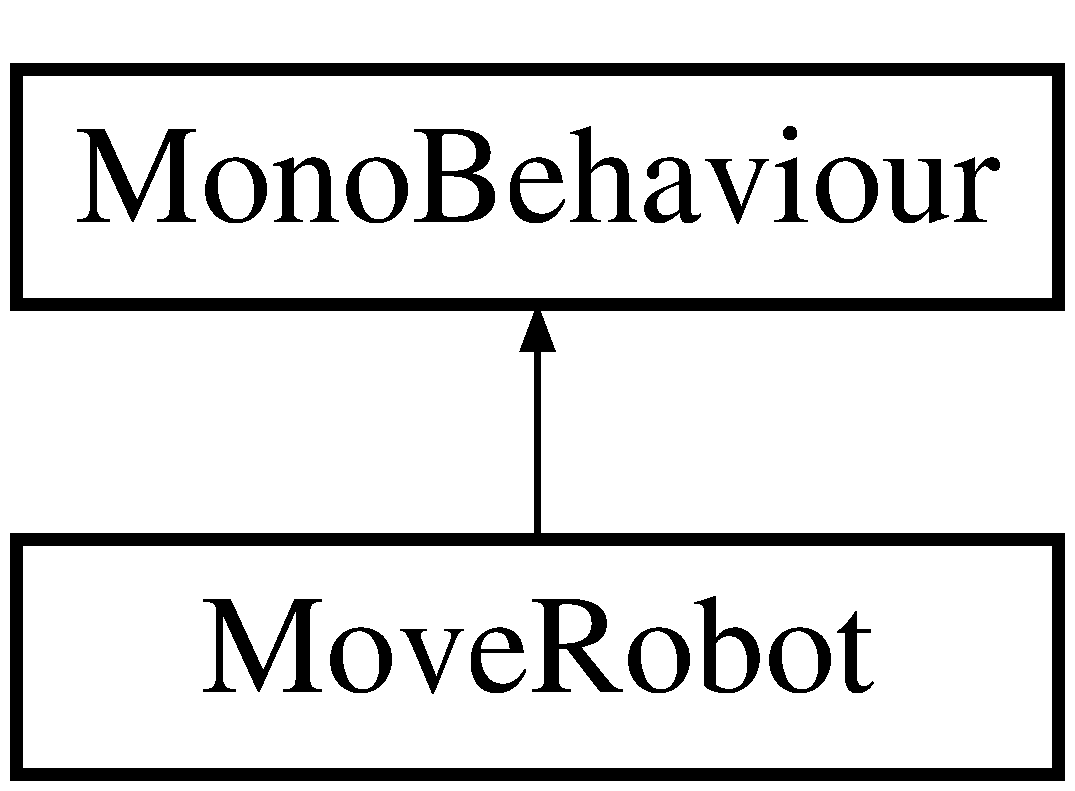
\includegraphics[height=2.000000cm]{class_move_robot}
\end{center}
\end{figure}
\subsection*{Public Member Functions}
\begin{DoxyCompactItemize}
\item 
void \mbox{\hyperlink{class_move_robot_acaa18eb45c2af4e040d08314ef6bfd77}{Start\+Moving}} (Vector3 destination, float speed=5f)
\begin{DoxyCompactList}\small\item\em Moves the robot to a destination specified in the param at a speed specified in the param (default 5f) \end{DoxyCompactList}\end{DoxyCompactItemize}
\subsection*{Private Member Functions}
\begin{DoxyCompactItemize}
\item 
void \mbox{\hyperlink{class_move_robot_a6f4c86e1a93a5f83cdde0d43998d48bd}{Start}} ()
\item 
void \mbox{\hyperlink{class_move_robot_a358d1401815e59ddae6edca2f7874b88}{Update}} ()
\end{DoxyCompactItemize}
\subsection*{Private Attributes}
\begin{DoxyCompactItemize}
\item 
bool \mbox{\hyperlink{class_move_robot_a3c7eeca97f62b1b3441b4f94854e6124}{m\+\_\+\+Is\+Moving}}
\item 
bool \mbox{\hyperlink{class_move_robot_a60f1a3b2d56b3c298e677d04d5a7b414}{m\+\_\+\+First\+Call}}
\item 
bool \mbox{\hyperlink{class_move_robot_a348c3db6da2394e433cb3bcd6cd9cb0b}{m\+\_\+\+Is\+Stopping}}
\item 
float \mbox{\hyperlink{class_move_robot_afaca031aa3c9f6a660d71c0e371f536f}{m\+\_\+\+Speed}} = 5f
\item 
Vector3 \mbox{\hyperlink{class_move_robot_a67cd9847aff3dc2e26cbb9cf3f27ab12}{m\+\_\+\+Dest}}
\item 
Game\+Object \mbox{\hyperlink{class_move_robot_a838c7823c5f333bb3583cce57fd9fcc8}{m\+\_\+\+Target\+Look\+At}}
\item 
float \mbox{\hyperlink{class_move_robot_a1be84318f7c7f9f5af8a2e84a2cf76b8}{m\+\_\+\+Stopping\+Distance}}
\item 
Animator \mbox{\hyperlink{class_move_robot_aef5a0d2a14b309e48c645400ec6b9be1}{m\+\_\+\+Robot\+Animator}}
\end{DoxyCompactItemize}


\subsection{Member Function Documentation}
\mbox{\Hypertarget{class_move_robot_a6f4c86e1a93a5f83cdde0d43998d48bd}\label{class_move_robot_a6f4c86e1a93a5f83cdde0d43998d48bd}} 
\index{Move\+Robot@{Move\+Robot}!Start@{Start}}
\index{Start@{Start}!Move\+Robot@{Move\+Robot}}
\subsubsection{\texorpdfstring{Start()}{Start()}}
{\footnotesize\ttfamily void Move\+Robot.\+Start (\begin{DoxyParamCaption}{ }\end{DoxyParamCaption})\hspace{0.3cm}{\ttfamily [private]}}

\mbox{\Hypertarget{class_move_robot_acaa18eb45c2af4e040d08314ef6bfd77}\label{class_move_robot_acaa18eb45c2af4e040d08314ef6bfd77}} 
\index{Move\+Robot@{Move\+Robot}!Start\+Moving@{Start\+Moving}}
\index{Start\+Moving@{Start\+Moving}!Move\+Robot@{Move\+Robot}}
\subsubsection{\texorpdfstring{Start\+Moving()}{StartMoving()}}
{\footnotesize\ttfamily void Move\+Robot.\+Start\+Moving (\begin{DoxyParamCaption}\item[{Vector3}]{destination,  }\item[{float}]{speed = {\ttfamily 5f} }\end{DoxyParamCaption})}



Moves the robot to a destination specified in the param at a speed specified in the param (default 5f) 


\begin{DoxyParams}{Parameters}
{\em destination} & destination to mvoe the robot to\\
\hline
{\em speed} & speed at which to move the robot\\
\hline
\end{DoxyParams}
\mbox{\Hypertarget{class_move_robot_a358d1401815e59ddae6edca2f7874b88}\label{class_move_robot_a358d1401815e59ddae6edca2f7874b88}} 
\index{Move\+Robot@{Move\+Robot}!Update@{Update}}
\index{Update@{Update}!Move\+Robot@{Move\+Robot}}
\subsubsection{\texorpdfstring{Update()}{Update()}}
{\footnotesize\ttfamily void Move\+Robot.\+Update (\begin{DoxyParamCaption}{ }\end{DoxyParamCaption})\hspace{0.3cm}{\ttfamily [private]}}



\subsection{Member Data Documentation}
\mbox{\Hypertarget{class_move_robot_a67cd9847aff3dc2e26cbb9cf3f27ab12}\label{class_move_robot_a67cd9847aff3dc2e26cbb9cf3f27ab12}} 
\index{Move\+Robot@{Move\+Robot}!m\+\_\+\+Dest@{m\+\_\+\+Dest}}
\index{m\+\_\+\+Dest@{m\+\_\+\+Dest}!Move\+Robot@{Move\+Robot}}
\subsubsection{\texorpdfstring{m\+\_\+\+Dest}{m\_Dest}}
{\footnotesize\ttfamily Vector3 Move\+Robot.\+m\+\_\+\+Dest\hspace{0.3cm}{\ttfamily [private]}}

\mbox{\Hypertarget{class_move_robot_a60f1a3b2d56b3c298e677d04d5a7b414}\label{class_move_robot_a60f1a3b2d56b3c298e677d04d5a7b414}} 
\index{Move\+Robot@{Move\+Robot}!m\+\_\+\+First\+Call@{m\+\_\+\+First\+Call}}
\index{m\+\_\+\+First\+Call@{m\+\_\+\+First\+Call}!Move\+Robot@{Move\+Robot}}
\subsubsection{\texorpdfstring{m\+\_\+\+First\+Call}{m\_FirstCall}}
{\footnotesize\ttfamily bool Move\+Robot.\+m\+\_\+\+First\+Call\hspace{0.3cm}{\ttfamily [private]}}

\mbox{\Hypertarget{class_move_robot_a3c7eeca97f62b1b3441b4f94854e6124}\label{class_move_robot_a3c7eeca97f62b1b3441b4f94854e6124}} 
\index{Move\+Robot@{Move\+Robot}!m\+\_\+\+Is\+Moving@{m\+\_\+\+Is\+Moving}}
\index{m\+\_\+\+Is\+Moving@{m\+\_\+\+Is\+Moving}!Move\+Robot@{Move\+Robot}}
\subsubsection{\texorpdfstring{m\+\_\+\+Is\+Moving}{m\_IsMoving}}
{\footnotesize\ttfamily bool Move\+Robot.\+m\+\_\+\+Is\+Moving\hspace{0.3cm}{\ttfamily [private]}}

\mbox{\Hypertarget{class_move_robot_a348c3db6da2394e433cb3bcd6cd9cb0b}\label{class_move_robot_a348c3db6da2394e433cb3bcd6cd9cb0b}} 
\index{Move\+Robot@{Move\+Robot}!m\+\_\+\+Is\+Stopping@{m\+\_\+\+Is\+Stopping}}
\index{m\+\_\+\+Is\+Stopping@{m\+\_\+\+Is\+Stopping}!Move\+Robot@{Move\+Robot}}
\subsubsection{\texorpdfstring{m\+\_\+\+Is\+Stopping}{m\_IsStopping}}
{\footnotesize\ttfamily bool Move\+Robot.\+m\+\_\+\+Is\+Stopping\hspace{0.3cm}{\ttfamily [private]}}

\mbox{\Hypertarget{class_move_robot_aef5a0d2a14b309e48c645400ec6b9be1}\label{class_move_robot_aef5a0d2a14b309e48c645400ec6b9be1}} 
\index{Move\+Robot@{Move\+Robot}!m\+\_\+\+Robot\+Animator@{m\+\_\+\+Robot\+Animator}}
\index{m\+\_\+\+Robot\+Animator@{m\+\_\+\+Robot\+Animator}!Move\+Robot@{Move\+Robot}}
\subsubsection{\texorpdfstring{m\+\_\+\+Robot\+Animator}{m\_RobotAnimator}}
{\footnotesize\ttfamily Animator Move\+Robot.\+m\+\_\+\+Robot\+Animator\hspace{0.3cm}{\ttfamily [private]}}

\mbox{\Hypertarget{class_move_robot_afaca031aa3c9f6a660d71c0e371f536f}\label{class_move_robot_afaca031aa3c9f6a660d71c0e371f536f}} 
\index{Move\+Robot@{Move\+Robot}!m\+\_\+\+Speed@{m\+\_\+\+Speed}}
\index{m\+\_\+\+Speed@{m\+\_\+\+Speed}!Move\+Robot@{Move\+Robot}}
\subsubsection{\texorpdfstring{m\+\_\+\+Speed}{m\_Speed}}
{\footnotesize\ttfamily float Move\+Robot.\+m\+\_\+\+Speed = 5f\hspace{0.3cm}{\ttfamily [private]}}

\mbox{\Hypertarget{class_move_robot_a1be84318f7c7f9f5af8a2e84a2cf76b8}\label{class_move_robot_a1be84318f7c7f9f5af8a2e84a2cf76b8}} 
\index{Move\+Robot@{Move\+Robot}!m\+\_\+\+Stopping\+Distance@{m\+\_\+\+Stopping\+Distance}}
\index{m\+\_\+\+Stopping\+Distance@{m\+\_\+\+Stopping\+Distance}!Move\+Robot@{Move\+Robot}}
\subsubsection{\texorpdfstring{m\+\_\+\+Stopping\+Distance}{m\_StoppingDistance}}
{\footnotesize\ttfamily float Move\+Robot.\+m\+\_\+\+Stopping\+Distance\hspace{0.3cm}{\ttfamily [private]}}

\mbox{\Hypertarget{class_move_robot_a838c7823c5f333bb3583cce57fd9fcc8}\label{class_move_robot_a838c7823c5f333bb3583cce57fd9fcc8}} 
\index{Move\+Robot@{Move\+Robot}!m\+\_\+\+Target\+Look\+At@{m\+\_\+\+Target\+Look\+At}}
\index{m\+\_\+\+Target\+Look\+At@{m\+\_\+\+Target\+Look\+At}!Move\+Robot@{Move\+Robot}}
\subsubsection{\texorpdfstring{m\+\_\+\+Target\+Look\+At}{m\_TargetLookAt}}
{\footnotesize\ttfamily Game\+Object Move\+Robot.\+m\+\_\+\+Target\+Look\+At\hspace{0.3cm}{\ttfamily [private]}}



The documentation for this class was generated from the following file\+:\begin{DoxyCompactItemize}
\item 
\mbox{\hyperlink{_move_robot_8cs}{Move\+Robot.\+cs}}\end{DoxyCompactItemize}

\hypertarget{class_v_r_standard_assets_1_1_utils_1_1_raycaster_v_r}{}\section{V\+R\+Standard\+Assets.\+Utils.\+Raycaster\+VR Class Reference}
\label{class_v_r_standard_assets_1_1_utils_1_1_raycaster_v_r}\index{V\+R\+Standard\+Assets.\+Utils.\+Raycaster\+VR@{V\+R\+Standard\+Assets.\+Utils.\+Raycaster\+VR}}
Inheritance diagram for V\+R\+Standard\+Assets.\+Utils.\+Raycaster\+VR\+:\begin{figure}[H]
\begin{center}
\leavevmode
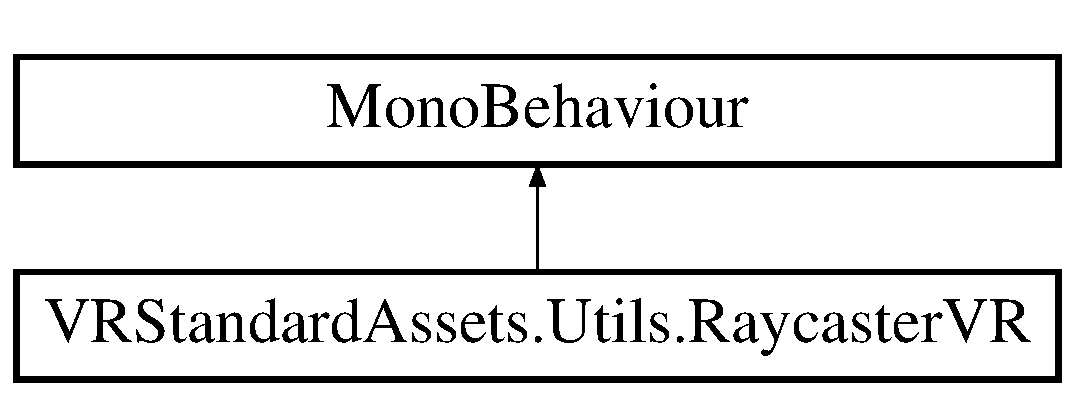
\includegraphics[height=2.000000cm]{class_v_r_standard_assets_1_1_utils_1_1_raycaster_v_r}
\end{center}
\end{figure}
\subsection*{Public Member Functions}
\begin{DoxyCompactItemize}
\item 
delegate void \mbox{\hyperlink{class_v_r_standard_assets_1_1_utils_1_1_raycaster_v_r_a208df26f1139ba566bd76ab13e654fac}{Ball\+Thrown}} ()
\item 
delegate void \mbox{\hyperlink{class_v_r_standard_assets_1_1_utils_1_1_raycaster_v_r_a85241158337110726e61258a3237752e}{Ball\+Picked\+Up}} ()
\item 
delegate void \mbox{\hyperlink{class_v_r_standard_assets_1_1_utils_1_1_raycaster_v_r_afa0e8c643d924f0f008364e153844e5f}{Ball\+Dropped}} ()
\item 
delegate void \mbox{\hyperlink{class_v_r_standard_assets_1_1_utils_1_1_raycaster_v_r_a68cab6ce8e6920717a4c08bc6f3992d8}{Stage3\+Button\+Clicked}} ()
\item 
void \mbox{\hyperlink{class_v_r_standard_assets_1_1_utils_1_1_raycaster_v_r_a9a87f20c50af01181912243fa8b88b21}{Grab\+Object}} ()
\begin{DoxyCompactList}\small\item\em Grabs an object and makes it a child of the controller model. \end{DoxyCompactList}\item 
void \mbox{\hyperlink{class_v_r_standard_assets_1_1_utils_1_1_raycaster_v_r_ad84bd58bab791d8ae7449eb923bb3153}{Release\+Object}} ()
\begin{DoxyCompactList}\small\item\em Releases object \end{DoxyCompactList}\item 
Game\+Object \mbox{\hyperlink{class_v_r_standard_assets_1_1_utils_1_1_raycaster_v_r_a5e7507b5485b5da01059538a932cafb2}{Get\+Target}} ()
\begin{DoxyCompactList}\small\item\em Returns the object the raycast is pointing to. Postcondition\+: Could return null if not raycasting on an object. \end{DoxyCompactList}\end{DoxyCompactItemize}
\subsection*{Public Attributes}
\begin{DoxyCompactItemize}
\item 
bool \mbox{\hyperlink{class_v_r_standard_assets_1_1_utils_1_1_raycaster_v_r_a729875cefaafc3d00b050d1b65b086f5}{m\+\_\+\+Holding\+Object}} = false
\item 
bool \mbox{\hyperlink{class_v_r_standard_assets_1_1_utils_1_1_raycaster_v_r_ad7f6af5f491c0d3955dcd7c712321f26}{m\+\_\+\+Override\+Default\+Reticle\+Controls}}
\end{DoxyCompactItemize}
\subsection*{Properties}
\begin{DoxyCompactItemize}
\item 
bool \mbox{\hyperlink{class_v_r_standard_assets_1_1_utils_1_1_raycaster_v_r_a4dfde4ab9f19a3c914e3d87ffe11a561}{Controller\+Is\+Connected}}\hspace{0.3cm}{\ttfamily  \mbox{[}get\mbox{]}}
\begin{DoxyCompactList}\small\item\em Returns if a controller is connected \end{DoxyCompactList}\item 
O\+V\+R\+Input.\+Controller \mbox{\hyperlink{class_v_r_standard_assets_1_1_utils_1_1_raycaster_v_r_a1de057b507bb494d68142465fa519145}{Controller}}\hspace{0.3cm}{\ttfamily  \mbox{[}get\mbox{]}}
\begin{DoxyCompactList}\small\item\em Returns the controller that is connected \end{DoxyCompactList}\end{DoxyCompactItemize}
\subsection*{Events}
\begin{DoxyCompactItemize}
\item 
static \mbox{\hyperlink{class_v_r_standard_assets_1_1_utils_1_1_raycaster_v_r_a208df26f1139ba566bd76ab13e654fac}{Ball\+Thrown}} \mbox{\hyperlink{class_v_r_standard_assets_1_1_utils_1_1_raycaster_v_r_a62d35bb4bf621e1d9b41991805091848}{e\+\_\+\+Object\+Was\+Thrown}}
\item 
static \mbox{\hyperlink{class_v_r_standard_assets_1_1_utils_1_1_raycaster_v_r_a85241158337110726e61258a3237752e}{Ball\+Picked\+Up}} \mbox{\hyperlink{class_v_r_standard_assets_1_1_utils_1_1_raycaster_v_r_ad264493543b631d078818d28706e21bb}{e\+\_\+\+Object\+Was\+Picked\+Up}}
\item 
static \mbox{\hyperlink{class_v_r_standard_assets_1_1_utils_1_1_raycaster_v_r_afa0e8c643d924f0f008364e153844e5f}{Ball\+Dropped}} \mbox{\hyperlink{class_v_r_standard_assets_1_1_utils_1_1_raycaster_v_r_ac6de8fe7e5086c4d89161e834153ece6}{e\+\_\+\+Object\+Was\+Dropped}}
\item 
static \mbox{\hyperlink{class_v_r_standard_assets_1_1_utils_1_1_raycaster_v_r_a68cab6ce8e6920717a4c08bc6f3992d8}{Stage3\+Button\+Clicked}} \mbox{\hyperlink{class_v_r_standard_assets_1_1_utils_1_1_raycaster_v_r_a6e380949eb3ae23d311cb3a4ae52313a}{e\+\_\+\+Button\+Clicked}}
\end{DoxyCompactItemize}
\subsection*{Private Types}
\begin{DoxyCompactItemize}
\item 
enum \mbox{\hyperlink{class_v_r_standard_assets_1_1_utils_1_1_raycaster_v_r_a6d511e0bf48faef93364d51b08d53f01}{Reticle\+State}} \{ \mbox{\hyperlink{class_v_r_standard_assets_1_1_utils_1_1_raycaster_v_r_a6d511e0bf48faef93364d51b08d53f01af8bde16b37ae953ddea395cb5b07d3b2}{Reticle\+State.\+Default\+State}}, 
\mbox{\hyperlink{class_v_r_standard_assets_1_1_utils_1_1_raycaster_v_r_a6d511e0bf48faef93364d51b08d53f01a163a551828daed4f057ad272119c197b}{Reticle\+State.\+Hover\+State}}, 
\mbox{\hyperlink{class_v_r_standard_assets_1_1_utils_1_1_raycaster_v_r_a6d511e0bf48faef93364d51b08d53f01ab4f8b825102708f811a24213fe1a1b8a}{Reticle\+State.\+Interacting\+State}}, 
\mbox{\hyperlink{class_v_r_standard_assets_1_1_utils_1_1_raycaster_v_r_a6d511e0bf48faef93364d51b08d53f01aedf260198e4d75d1cb3c7588f7380120}{Reticle\+State.\+Invalid\+State}}
 \}
\end{DoxyCompactItemize}
\subsection*{Private Member Functions}
\begin{DoxyCompactItemize}
\item 
void \mbox{\hyperlink{class_v_r_standard_assets_1_1_utils_1_1_raycaster_v_r_a2a39009ca324b8f349777d3c78efa239}{Start}} ()
\item 
void \mbox{\hyperlink{class_v_r_standard_assets_1_1_utils_1_1_raycaster_v_r_a5073e9a8e781617a65ce06ebff8a0b5a}{Update}} ()
\item 
void \mbox{\hyperlink{class_v_r_standard_assets_1_1_utils_1_1_raycaster_v_r_a736d463c2ce54e52c904283f15a852b4}{Raycast}} ()
\begin{DoxyCompactList}\small\item\em Function will emit a raycast from the camera or controller. It will set {\ttfamily m\+\_\+\+Target} to the current object being raycast on. Inside this function is also where the events are triggered and objects are interacted with (held/thrown/clicked on). \end{DoxyCompactList}\item 
void \mbox{\hyperlink{class_v_r_standard_assets_1_1_utils_1_1_raycaster_v_r_ac2d0ad7b65663683c3a01c9d57f6b790}{Throw\+Object}} (int dir)
\begin{DoxyCompactList}\small\item\em Throws an object Precondition\+: param dir is 1 or -\/1. Use 1 for forward and -\/1 for backward. \end{DoxyCompactList}\end{DoxyCompactItemize}
\subsection*{Private Attributes}
\begin{DoxyCompactItemize}
\item 
Transform \mbox{\hyperlink{class_v_r_standard_assets_1_1_utils_1_1_raycaster_v_r_a31175f7387fee9ad2c589980f8fb208b}{m\+\_\+\+Camera}}
\item 
Layer\+Mask \mbox{\hyperlink{class_v_r_standard_assets_1_1_utils_1_1_raycaster_v_r_a1d35cc7d2ca61987f02ec95f8fad7fa1}{m\+\_\+\+Exclusion\+Layers}}
\item 
\mbox{\hyperlink{class_v_r_standard_assets_1_1_utils_1_1_reticle}{Reticle}} \mbox{\hyperlink{class_v_r_standard_assets_1_1_utils_1_1_raycaster_v_r_a2550a8e10afb25305545ddbaaa262b6c}{m\+\_\+\+Reticle}}
\item 
bool \mbox{\hyperlink{class_v_r_standard_assets_1_1_utils_1_1_raycaster_v_r_aa4960007d414cecc535ce5b23943d24a}{m\+\_\+\+Show\+Debug\+Ray}}
\item 
float \mbox{\hyperlink{class_v_r_standard_assets_1_1_utils_1_1_raycaster_v_r_a10e84a6cc342262543703474063a477e}{m\+\_\+\+Debug\+Ray\+Length}} = 5f
\item 
float \mbox{\hyperlink{class_v_r_standard_assets_1_1_utils_1_1_raycaster_v_r_a3de25fdc1c66f09bb08916fa8f974371}{m\+\_\+\+Debug\+Ray\+Duration}} = 1f
\item 
float \mbox{\hyperlink{class_v_r_standard_assets_1_1_utils_1_1_raycaster_v_r_ac8a6f36aeb0994c4a02cf61bf9ef6a69}{m\+\_\+\+Ray\+Length}} = 500f
\item 
Game\+Object \mbox{\hyperlink{class_v_r_standard_assets_1_1_utils_1_1_raycaster_v_r_a81006ae23a74ee04b8a8ea55ba30ed33}{m\+\_\+\+Direction}}
\item 
float \mbox{\hyperlink{class_v_r_standard_assets_1_1_utils_1_1_raycaster_v_r_a27a44b2b0607f850cecccc8e511c9eba}{force}} = 1000f
\item 
Transform \mbox{\hyperlink{class_v_r_standard_assets_1_1_utils_1_1_raycaster_v_r_a3c79624027b0bd0f129e49dc3a9662be}{m\+\_\+\+Tracking\+Space}} = null
\item 
Game\+Object \mbox{\hyperlink{class_v_r_standard_assets_1_1_utils_1_1_raycaster_v_r_a6f5ccf9d919b2aecad32fd8c536833be}{m\+\_\+\+Controller\+Model}}
\item 
Vector3 \mbox{\hyperlink{class_v_r_standard_assets_1_1_utils_1_1_raycaster_v_r_a5ade6b07c95cfa98fdcd4a0d8ead854c}{m\+\_\+\+Offset\+Vector}}
\item 
Game\+Object \mbox{\hyperlink{class_v_r_standard_assets_1_1_utils_1_1_raycaster_v_r_a643af822a4a662ceb4a8b3dc42b71a7f}{m\+\_\+\+Target}}
\item 
Game\+Object \mbox{\hyperlink{class_v_r_standard_assets_1_1_utils_1_1_raycaster_v_r_af5246fa12faee8799d34c98da4d43e0a}{m\+\_\+\+Object\+Held}}
\item 
float \mbox{\hyperlink{class_v_r_standard_assets_1_1_utils_1_1_raycaster_v_r_a1fac3f431a4947b5ff30915004be4491}{m\+\_\+\+Trigger\+Pull\+Timer}} = 0f
\item 
bool \mbox{\hyperlink{class_v_r_standard_assets_1_1_utils_1_1_raycaster_v_r_ab07ed62bf6158d940e00efffa6269784}{m\+\_\+\+Object\+Released}} = true
\item 
float \mbox{\hyperlink{class_v_r_standard_assets_1_1_utils_1_1_raycaster_v_r_a73cae4edd2893e9168ab029350ae10e2}{m\+\_\+\+Reticle\+State\+Timer}} = 0f
\item 
\mbox{\hyperlink{class_v_r_standard_assets_1_1_utils_1_1_raycaster_v_r_a6d511e0bf48faef93364d51b08d53f01}{Reticle\+State}} \mbox{\hyperlink{class_v_r_standard_assets_1_1_utils_1_1_raycaster_v_r_a57ab24a6eda192ebce83cf84e580265c}{m\+\_\+\+Current\+Reticle\+State}}
\end{DoxyCompactItemize}


\subsection{Member Enumeration Documentation}
\mbox{\Hypertarget{class_v_r_standard_assets_1_1_utils_1_1_raycaster_v_r_a6d511e0bf48faef93364d51b08d53f01}\label{class_v_r_standard_assets_1_1_utils_1_1_raycaster_v_r_a6d511e0bf48faef93364d51b08d53f01}} 
\index{V\+R\+Standard\+Assets\+::\+Utils\+::\+Raycaster\+VR@{V\+R\+Standard\+Assets\+::\+Utils\+::\+Raycaster\+VR}!Reticle\+State@{Reticle\+State}}
\index{Reticle\+State@{Reticle\+State}!V\+R\+Standard\+Assets\+::\+Utils\+::\+Raycaster\+VR@{V\+R\+Standard\+Assets\+::\+Utils\+::\+Raycaster\+VR}}
\subsubsection{\texorpdfstring{Reticle\+State}{ReticleState}}
{\footnotesize\ttfamily enum \mbox{\hyperlink{class_v_r_standard_assets_1_1_utils_1_1_raycaster_v_r_a6d511e0bf48faef93364d51b08d53f01}{V\+R\+Standard\+Assets.\+Utils.\+Raycaster\+V\+R.\+Reticle\+State}}\hspace{0.3cm}{\ttfamily [strong]}, {\ttfamily [private]}}

\begin{DoxyEnumFields}{Enumerator}
\raisebox{\heightof{T}}[0pt][0pt]{\index{Default\+State@{Default\+State}!V\+R\+Standard\+Assets\+::\+Utils\+::\+Raycaster\+VR@{V\+R\+Standard\+Assets\+::\+Utils\+::\+Raycaster\+VR}}\index{V\+R\+Standard\+Assets\+::\+Utils\+::\+Raycaster\+VR@{V\+R\+Standard\+Assets\+::\+Utils\+::\+Raycaster\+VR}!Default\+State@{Default\+State}}}\mbox{\Hypertarget{class_v_r_standard_assets_1_1_utils_1_1_raycaster_v_r_a6d511e0bf48faef93364d51b08d53f01af8bde16b37ae953ddea395cb5b07d3b2}\label{class_v_r_standard_assets_1_1_utils_1_1_raycaster_v_r_a6d511e0bf48faef93364d51b08d53f01af8bde16b37ae953ddea395cb5b07d3b2}} 
Default\+State&\\
\hline

\raisebox{\heightof{T}}[0pt][0pt]{\index{Hover\+State@{Hover\+State}!V\+R\+Standard\+Assets\+::\+Utils\+::\+Raycaster\+VR@{V\+R\+Standard\+Assets\+::\+Utils\+::\+Raycaster\+VR}}\index{V\+R\+Standard\+Assets\+::\+Utils\+::\+Raycaster\+VR@{V\+R\+Standard\+Assets\+::\+Utils\+::\+Raycaster\+VR}!Hover\+State@{Hover\+State}}}\mbox{\Hypertarget{class_v_r_standard_assets_1_1_utils_1_1_raycaster_v_r_a6d511e0bf48faef93364d51b08d53f01a163a551828daed4f057ad272119c197b}\label{class_v_r_standard_assets_1_1_utils_1_1_raycaster_v_r_a6d511e0bf48faef93364d51b08d53f01a163a551828daed4f057ad272119c197b}} 
Hover\+State&\\
\hline

\raisebox{\heightof{T}}[0pt][0pt]{\index{Interacting\+State@{Interacting\+State}!V\+R\+Standard\+Assets\+::\+Utils\+::\+Raycaster\+VR@{V\+R\+Standard\+Assets\+::\+Utils\+::\+Raycaster\+VR}}\index{V\+R\+Standard\+Assets\+::\+Utils\+::\+Raycaster\+VR@{V\+R\+Standard\+Assets\+::\+Utils\+::\+Raycaster\+VR}!Interacting\+State@{Interacting\+State}}}\mbox{\Hypertarget{class_v_r_standard_assets_1_1_utils_1_1_raycaster_v_r_a6d511e0bf48faef93364d51b08d53f01ab4f8b825102708f811a24213fe1a1b8a}\label{class_v_r_standard_assets_1_1_utils_1_1_raycaster_v_r_a6d511e0bf48faef93364d51b08d53f01ab4f8b825102708f811a24213fe1a1b8a}} 
Interacting\+State&\\
\hline

\raisebox{\heightof{T}}[0pt][0pt]{\index{Invalid\+State@{Invalid\+State}!V\+R\+Standard\+Assets\+::\+Utils\+::\+Raycaster\+VR@{V\+R\+Standard\+Assets\+::\+Utils\+::\+Raycaster\+VR}}\index{V\+R\+Standard\+Assets\+::\+Utils\+::\+Raycaster\+VR@{V\+R\+Standard\+Assets\+::\+Utils\+::\+Raycaster\+VR}!Invalid\+State@{Invalid\+State}}}\mbox{\Hypertarget{class_v_r_standard_assets_1_1_utils_1_1_raycaster_v_r_a6d511e0bf48faef93364d51b08d53f01aedf260198e4d75d1cb3c7588f7380120}\label{class_v_r_standard_assets_1_1_utils_1_1_raycaster_v_r_a6d511e0bf48faef93364d51b08d53f01aedf260198e4d75d1cb3c7588f7380120}} 
Invalid\+State&\\
\hline

\end{DoxyEnumFields}


\subsection{Member Function Documentation}
\mbox{\Hypertarget{class_v_r_standard_assets_1_1_utils_1_1_raycaster_v_r_afa0e8c643d924f0f008364e153844e5f}\label{class_v_r_standard_assets_1_1_utils_1_1_raycaster_v_r_afa0e8c643d924f0f008364e153844e5f}} 
\index{V\+R\+Standard\+Assets\+::\+Utils\+::\+Raycaster\+VR@{V\+R\+Standard\+Assets\+::\+Utils\+::\+Raycaster\+VR}!Ball\+Dropped@{Ball\+Dropped}}
\index{Ball\+Dropped@{Ball\+Dropped}!V\+R\+Standard\+Assets\+::\+Utils\+::\+Raycaster\+VR@{V\+R\+Standard\+Assets\+::\+Utils\+::\+Raycaster\+VR}}
\subsubsection{\texorpdfstring{Ball\+Dropped()}{BallDropped()}}
{\footnotesize\ttfamily delegate void V\+R\+Standard\+Assets.\+Utils.\+Raycaster\+V\+R.\+Ball\+Dropped (\begin{DoxyParamCaption}{ }\end{DoxyParamCaption})}

\mbox{\Hypertarget{class_v_r_standard_assets_1_1_utils_1_1_raycaster_v_r_a85241158337110726e61258a3237752e}\label{class_v_r_standard_assets_1_1_utils_1_1_raycaster_v_r_a85241158337110726e61258a3237752e}} 
\index{V\+R\+Standard\+Assets\+::\+Utils\+::\+Raycaster\+VR@{V\+R\+Standard\+Assets\+::\+Utils\+::\+Raycaster\+VR}!Ball\+Picked\+Up@{Ball\+Picked\+Up}}
\index{Ball\+Picked\+Up@{Ball\+Picked\+Up}!V\+R\+Standard\+Assets\+::\+Utils\+::\+Raycaster\+VR@{V\+R\+Standard\+Assets\+::\+Utils\+::\+Raycaster\+VR}}
\subsubsection{\texorpdfstring{Ball\+Picked\+Up()}{BallPickedUp()}}
{\footnotesize\ttfamily delegate void V\+R\+Standard\+Assets.\+Utils.\+Raycaster\+V\+R.\+Ball\+Picked\+Up (\begin{DoxyParamCaption}{ }\end{DoxyParamCaption})}

\mbox{\Hypertarget{class_v_r_standard_assets_1_1_utils_1_1_raycaster_v_r_a208df26f1139ba566bd76ab13e654fac}\label{class_v_r_standard_assets_1_1_utils_1_1_raycaster_v_r_a208df26f1139ba566bd76ab13e654fac}} 
\index{V\+R\+Standard\+Assets\+::\+Utils\+::\+Raycaster\+VR@{V\+R\+Standard\+Assets\+::\+Utils\+::\+Raycaster\+VR}!Ball\+Thrown@{Ball\+Thrown}}
\index{Ball\+Thrown@{Ball\+Thrown}!V\+R\+Standard\+Assets\+::\+Utils\+::\+Raycaster\+VR@{V\+R\+Standard\+Assets\+::\+Utils\+::\+Raycaster\+VR}}
\subsubsection{\texorpdfstring{Ball\+Thrown()}{BallThrown()}}
{\footnotesize\ttfamily delegate void V\+R\+Standard\+Assets.\+Utils.\+Raycaster\+V\+R.\+Ball\+Thrown (\begin{DoxyParamCaption}{ }\end{DoxyParamCaption})}

\mbox{\Hypertarget{class_v_r_standard_assets_1_1_utils_1_1_raycaster_v_r_a5e7507b5485b5da01059538a932cafb2}\label{class_v_r_standard_assets_1_1_utils_1_1_raycaster_v_r_a5e7507b5485b5da01059538a932cafb2}} 
\index{V\+R\+Standard\+Assets\+::\+Utils\+::\+Raycaster\+VR@{V\+R\+Standard\+Assets\+::\+Utils\+::\+Raycaster\+VR}!Get\+Target@{Get\+Target}}
\index{Get\+Target@{Get\+Target}!V\+R\+Standard\+Assets\+::\+Utils\+::\+Raycaster\+VR@{V\+R\+Standard\+Assets\+::\+Utils\+::\+Raycaster\+VR}}
\subsubsection{\texorpdfstring{Get\+Target()}{GetTarget()}}
{\footnotesize\ttfamily Game\+Object V\+R\+Standard\+Assets.\+Utils.\+Raycaster\+V\+R.\+Get\+Target (\begin{DoxyParamCaption}{ }\end{DoxyParamCaption})}



Returns the object the raycast is pointing to. Postcondition\+: Could return null if not raycasting on an object. 

\begin{DoxyReturn}{Returns}
The target being pointed at.
\end{DoxyReturn}
\mbox{\Hypertarget{class_v_r_standard_assets_1_1_utils_1_1_raycaster_v_r_a9a87f20c50af01181912243fa8b88b21}\label{class_v_r_standard_assets_1_1_utils_1_1_raycaster_v_r_a9a87f20c50af01181912243fa8b88b21}} 
\index{V\+R\+Standard\+Assets\+::\+Utils\+::\+Raycaster\+VR@{V\+R\+Standard\+Assets\+::\+Utils\+::\+Raycaster\+VR}!Grab\+Object@{Grab\+Object}}
\index{Grab\+Object@{Grab\+Object}!V\+R\+Standard\+Assets\+::\+Utils\+::\+Raycaster\+VR@{V\+R\+Standard\+Assets\+::\+Utils\+::\+Raycaster\+VR}}
\subsubsection{\texorpdfstring{Grab\+Object()}{GrabObject()}}
{\footnotesize\ttfamily void V\+R\+Standard\+Assets.\+Utils.\+Raycaster\+V\+R.\+Grab\+Object (\begin{DoxyParamCaption}{ }\end{DoxyParamCaption})}



Grabs an object and makes it a child of the controller model. 

\mbox{\Hypertarget{class_v_r_standard_assets_1_1_utils_1_1_raycaster_v_r_a736d463c2ce54e52c904283f15a852b4}\label{class_v_r_standard_assets_1_1_utils_1_1_raycaster_v_r_a736d463c2ce54e52c904283f15a852b4}} 
\index{V\+R\+Standard\+Assets\+::\+Utils\+::\+Raycaster\+VR@{V\+R\+Standard\+Assets\+::\+Utils\+::\+Raycaster\+VR}!Raycast@{Raycast}}
\index{Raycast@{Raycast}!V\+R\+Standard\+Assets\+::\+Utils\+::\+Raycaster\+VR@{V\+R\+Standard\+Assets\+::\+Utils\+::\+Raycaster\+VR}}
\subsubsection{\texorpdfstring{Raycast()}{Raycast()}}
{\footnotesize\ttfamily void V\+R\+Standard\+Assets.\+Utils.\+Raycaster\+V\+R.\+Raycast (\begin{DoxyParamCaption}{ }\end{DoxyParamCaption})\hspace{0.3cm}{\ttfamily [private]}}



Function will emit a raycast from the camera or controller. It will set {\ttfamily m\+\_\+\+Target} to the current object being raycast on. Inside this function is also where the events are triggered and objects are interacted with (held/thrown/clicked on). 

\mbox{\Hypertarget{class_v_r_standard_assets_1_1_utils_1_1_raycaster_v_r_ad84bd58bab791d8ae7449eb923bb3153}\label{class_v_r_standard_assets_1_1_utils_1_1_raycaster_v_r_ad84bd58bab791d8ae7449eb923bb3153}} 
\index{V\+R\+Standard\+Assets\+::\+Utils\+::\+Raycaster\+VR@{V\+R\+Standard\+Assets\+::\+Utils\+::\+Raycaster\+VR}!Release\+Object@{Release\+Object}}
\index{Release\+Object@{Release\+Object}!V\+R\+Standard\+Assets\+::\+Utils\+::\+Raycaster\+VR@{V\+R\+Standard\+Assets\+::\+Utils\+::\+Raycaster\+VR}}
\subsubsection{\texorpdfstring{Release\+Object()}{ReleaseObject()}}
{\footnotesize\ttfamily void V\+R\+Standard\+Assets.\+Utils.\+Raycaster\+V\+R.\+Release\+Object (\begin{DoxyParamCaption}{ }\end{DoxyParamCaption})}



Releases object 

\mbox{\Hypertarget{class_v_r_standard_assets_1_1_utils_1_1_raycaster_v_r_a68cab6ce8e6920717a4c08bc6f3992d8}\label{class_v_r_standard_assets_1_1_utils_1_1_raycaster_v_r_a68cab6ce8e6920717a4c08bc6f3992d8}} 
\index{V\+R\+Standard\+Assets\+::\+Utils\+::\+Raycaster\+VR@{V\+R\+Standard\+Assets\+::\+Utils\+::\+Raycaster\+VR}!Stage3\+Button\+Clicked@{Stage3\+Button\+Clicked}}
\index{Stage3\+Button\+Clicked@{Stage3\+Button\+Clicked}!V\+R\+Standard\+Assets\+::\+Utils\+::\+Raycaster\+VR@{V\+R\+Standard\+Assets\+::\+Utils\+::\+Raycaster\+VR}}
\subsubsection{\texorpdfstring{Stage3\+Button\+Clicked()}{Stage3ButtonClicked()}}
{\footnotesize\ttfamily delegate void V\+R\+Standard\+Assets.\+Utils.\+Raycaster\+V\+R.\+Stage3\+Button\+Clicked (\begin{DoxyParamCaption}{ }\end{DoxyParamCaption})}

\mbox{\Hypertarget{class_v_r_standard_assets_1_1_utils_1_1_raycaster_v_r_a2a39009ca324b8f349777d3c78efa239}\label{class_v_r_standard_assets_1_1_utils_1_1_raycaster_v_r_a2a39009ca324b8f349777d3c78efa239}} 
\index{V\+R\+Standard\+Assets\+::\+Utils\+::\+Raycaster\+VR@{V\+R\+Standard\+Assets\+::\+Utils\+::\+Raycaster\+VR}!Start@{Start}}
\index{Start@{Start}!V\+R\+Standard\+Assets\+::\+Utils\+::\+Raycaster\+VR@{V\+R\+Standard\+Assets\+::\+Utils\+::\+Raycaster\+VR}}
\subsubsection{\texorpdfstring{Start()}{Start()}}
{\footnotesize\ttfamily void V\+R\+Standard\+Assets.\+Utils.\+Raycaster\+V\+R.\+Start (\begin{DoxyParamCaption}{ }\end{DoxyParamCaption})\hspace{0.3cm}{\ttfamily [private]}}

\mbox{\Hypertarget{class_v_r_standard_assets_1_1_utils_1_1_raycaster_v_r_ac2d0ad7b65663683c3a01c9d57f6b790}\label{class_v_r_standard_assets_1_1_utils_1_1_raycaster_v_r_ac2d0ad7b65663683c3a01c9d57f6b790}} 
\index{V\+R\+Standard\+Assets\+::\+Utils\+::\+Raycaster\+VR@{V\+R\+Standard\+Assets\+::\+Utils\+::\+Raycaster\+VR}!Throw\+Object@{Throw\+Object}}
\index{Throw\+Object@{Throw\+Object}!V\+R\+Standard\+Assets\+::\+Utils\+::\+Raycaster\+VR@{V\+R\+Standard\+Assets\+::\+Utils\+::\+Raycaster\+VR}}
\subsubsection{\texorpdfstring{Throw\+Object()}{ThrowObject()}}
{\footnotesize\ttfamily void V\+R\+Standard\+Assets.\+Utils.\+Raycaster\+V\+R.\+Throw\+Object (\begin{DoxyParamCaption}\item[{int}]{dir }\end{DoxyParamCaption})\hspace{0.3cm}{\ttfamily [private]}}



Throws an object Precondition\+: param dir is 1 or -\/1. Use 1 for forward and -\/1 for backward. 


\begin{DoxyParams}{Parameters}
{\em dir} & Direction to throw the object. Use 1 for forward and -\/1 for backward.\\
\hline
\end{DoxyParams}
\mbox{\Hypertarget{class_v_r_standard_assets_1_1_utils_1_1_raycaster_v_r_a5073e9a8e781617a65ce06ebff8a0b5a}\label{class_v_r_standard_assets_1_1_utils_1_1_raycaster_v_r_a5073e9a8e781617a65ce06ebff8a0b5a}} 
\index{V\+R\+Standard\+Assets\+::\+Utils\+::\+Raycaster\+VR@{V\+R\+Standard\+Assets\+::\+Utils\+::\+Raycaster\+VR}!Update@{Update}}
\index{Update@{Update}!V\+R\+Standard\+Assets\+::\+Utils\+::\+Raycaster\+VR@{V\+R\+Standard\+Assets\+::\+Utils\+::\+Raycaster\+VR}}
\subsubsection{\texorpdfstring{Update()}{Update()}}
{\footnotesize\ttfamily void V\+R\+Standard\+Assets.\+Utils.\+Raycaster\+V\+R.\+Update (\begin{DoxyParamCaption}{ }\end{DoxyParamCaption})\hspace{0.3cm}{\ttfamily [private]}}



\subsection{Member Data Documentation}
\mbox{\Hypertarget{class_v_r_standard_assets_1_1_utils_1_1_raycaster_v_r_a27a44b2b0607f850cecccc8e511c9eba}\label{class_v_r_standard_assets_1_1_utils_1_1_raycaster_v_r_a27a44b2b0607f850cecccc8e511c9eba}} 
\index{V\+R\+Standard\+Assets\+::\+Utils\+::\+Raycaster\+VR@{V\+R\+Standard\+Assets\+::\+Utils\+::\+Raycaster\+VR}!force@{force}}
\index{force@{force}!V\+R\+Standard\+Assets\+::\+Utils\+::\+Raycaster\+VR@{V\+R\+Standard\+Assets\+::\+Utils\+::\+Raycaster\+VR}}
\subsubsection{\texorpdfstring{force}{force}}
{\footnotesize\ttfamily float V\+R\+Standard\+Assets.\+Utils.\+Raycaster\+V\+R.\+force = 1000f\hspace{0.3cm}{\ttfamily [private]}}

\mbox{\Hypertarget{class_v_r_standard_assets_1_1_utils_1_1_raycaster_v_r_a31175f7387fee9ad2c589980f8fb208b}\label{class_v_r_standard_assets_1_1_utils_1_1_raycaster_v_r_a31175f7387fee9ad2c589980f8fb208b}} 
\index{V\+R\+Standard\+Assets\+::\+Utils\+::\+Raycaster\+VR@{V\+R\+Standard\+Assets\+::\+Utils\+::\+Raycaster\+VR}!m\+\_\+\+Camera@{m\+\_\+\+Camera}}
\index{m\+\_\+\+Camera@{m\+\_\+\+Camera}!V\+R\+Standard\+Assets\+::\+Utils\+::\+Raycaster\+VR@{V\+R\+Standard\+Assets\+::\+Utils\+::\+Raycaster\+VR}}
\subsubsection{\texorpdfstring{m\+\_\+\+Camera}{m\_Camera}}
{\footnotesize\ttfamily Transform V\+R\+Standard\+Assets.\+Utils.\+Raycaster\+V\+R.\+m\+\_\+\+Camera\hspace{0.3cm}{\ttfamily [private]}}

\mbox{\Hypertarget{class_v_r_standard_assets_1_1_utils_1_1_raycaster_v_r_a6f5ccf9d919b2aecad32fd8c536833be}\label{class_v_r_standard_assets_1_1_utils_1_1_raycaster_v_r_a6f5ccf9d919b2aecad32fd8c536833be}} 
\index{V\+R\+Standard\+Assets\+::\+Utils\+::\+Raycaster\+VR@{V\+R\+Standard\+Assets\+::\+Utils\+::\+Raycaster\+VR}!m\+\_\+\+Controller\+Model@{m\+\_\+\+Controller\+Model}}
\index{m\+\_\+\+Controller\+Model@{m\+\_\+\+Controller\+Model}!V\+R\+Standard\+Assets\+::\+Utils\+::\+Raycaster\+VR@{V\+R\+Standard\+Assets\+::\+Utils\+::\+Raycaster\+VR}}
\subsubsection{\texorpdfstring{m\+\_\+\+Controller\+Model}{m\_ControllerModel}}
{\footnotesize\ttfamily Game\+Object V\+R\+Standard\+Assets.\+Utils.\+Raycaster\+V\+R.\+m\+\_\+\+Controller\+Model\hspace{0.3cm}{\ttfamily [private]}}

\mbox{\Hypertarget{class_v_r_standard_assets_1_1_utils_1_1_raycaster_v_r_a57ab24a6eda192ebce83cf84e580265c}\label{class_v_r_standard_assets_1_1_utils_1_1_raycaster_v_r_a57ab24a6eda192ebce83cf84e580265c}} 
\index{V\+R\+Standard\+Assets\+::\+Utils\+::\+Raycaster\+VR@{V\+R\+Standard\+Assets\+::\+Utils\+::\+Raycaster\+VR}!m\+\_\+\+Current\+Reticle\+State@{m\+\_\+\+Current\+Reticle\+State}}
\index{m\+\_\+\+Current\+Reticle\+State@{m\+\_\+\+Current\+Reticle\+State}!V\+R\+Standard\+Assets\+::\+Utils\+::\+Raycaster\+VR@{V\+R\+Standard\+Assets\+::\+Utils\+::\+Raycaster\+VR}}
\subsubsection{\texorpdfstring{m\+\_\+\+Current\+Reticle\+State}{m\_CurrentReticleState}}
{\footnotesize\ttfamily \mbox{\hyperlink{class_v_r_standard_assets_1_1_utils_1_1_raycaster_v_r_a6d511e0bf48faef93364d51b08d53f01}{Reticle\+State}} V\+R\+Standard\+Assets.\+Utils.\+Raycaster\+V\+R.\+m\+\_\+\+Current\+Reticle\+State\hspace{0.3cm}{\ttfamily [private]}}

\mbox{\Hypertarget{class_v_r_standard_assets_1_1_utils_1_1_raycaster_v_r_a3de25fdc1c66f09bb08916fa8f974371}\label{class_v_r_standard_assets_1_1_utils_1_1_raycaster_v_r_a3de25fdc1c66f09bb08916fa8f974371}} 
\index{V\+R\+Standard\+Assets\+::\+Utils\+::\+Raycaster\+VR@{V\+R\+Standard\+Assets\+::\+Utils\+::\+Raycaster\+VR}!m\+\_\+\+Debug\+Ray\+Duration@{m\+\_\+\+Debug\+Ray\+Duration}}
\index{m\+\_\+\+Debug\+Ray\+Duration@{m\+\_\+\+Debug\+Ray\+Duration}!V\+R\+Standard\+Assets\+::\+Utils\+::\+Raycaster\+VR@{V\+R\+Standard\+Assets\+::\+Utils\+::\+Raycaster\+VR}}
\subsubsection{\texorpdfstring{m\+\_\+\+Debug\+Ray\+Duration}{m\_DebugRayDuration}}
{\footnotesize\ttfamily float V\+R\+Standard\+Assets.\+Utils.\+Raycaster\+V\+R.\+m\+\_\+\+Debug\+Ray\+Duration = 1f\hspace{0.3cm}{\ttfamily [private]}}

\mbox{\Hypertarget{class_v_r_standard_assets_1_1_utils_1_1_raycaster_v_r_a10e84a6cc342262543703474063a477e}\label{class_v_r_standard_assets_1_1_utils_1_1_raycaster_v_r_a10e84a6cc342262543703474063a477e}} 
\index{V\+R\+Standard\+Assets\+::\+Utils\+::\+Raycaster\+VR@{V\+R\+Standard\+Assets\+::\+Utils\+::\+Raycaster\+VR}!m\+\_\+\+Debug\+Ray\+Length@{m\+\_\+\+Debug\+Ray\+Length}}
\index{m\+\_\+\+Debug\+Ray\+Length@{m\+\_\+\+Debug\+Ray\+Length}!V\+R\+Standard\+Assets\+::\+Utils\+::\+Raycaster\+VR@{V\+R\+Standard\+Assets\+::\+Utils\+::\+Raycaster\+VR}}
\subsubsection{\texorpdfstring{m\+\_\+\+Debug\+Ray\+Length}{m\_DebugRayLength}}
{\footnotesize\ttfamily float V\+R\+Standard\+Assets.\+Utils.\+Raycaster\+V\+R.\+m\+\_\+\+Debug\+Ray\+Length = 5f\hspace{0.3cm}{\ttfamily [private]}}

\mbox{\Hypertarget{class_v_r_standard_assets_1_1_utils_1_1_raycaster_v_r_a81006ae23a74ee04b8a8ea55ba30ed33}\label{class_v_r_standard_assets_1_1_utils_1_1_raycaster_v_r_a81006ae23a74ee04b8a8ea55ba30ed33}} 
\index{V\+R\+Standard\+Assets\+::\+Utils\+::\+Raycaster\+VR@{V\+R\+Standard\+Assets\+::\+Utils\+::\+Raycaster\+VR}!m\+\_\+\+Direction@{m\+\_\+\+Direction}}
\index{m\+\_\+\+Direction@{m\+\_\+\+Direction}!V\+R\+Standard\+Assets\+::\+Utils\+::\+Raycaster\+VR@{V\+R\+Standard\+Assets\+::\+Utils\+::\+Raycaster\+VR}}
\subsubsection{\texorpdfstring{m\+\_\+\+Direction}{m\_Direction}}
{\footnotesize\ttfamily Game\+Object V\+R\+Standard\+Assets.\+Utils.\+Raycaster\+V\+R.\+m\+\_\+\+Direction\hspace{0.3cm}{\ttfamily [private]}}

\mbox{\Hypertarget{class_v_r_standard_assets_1_1_utils_1_1_raycaster_v_r_a1d35cc7d2ca61987f02ec95f8fad7fa1}\label{class_v_r_standard_assets_1_1_utils_1_1_raycaster_v_r_a1d35cc7d2ca61987f02ec95f8fad7fa1}} 
\index{V\+R\+Standard\+Assets\+::\+Utils\+::\+Raycaster\+VR@{V\+R\+Standard\+Assets\+::\+Utils\+::\+Raycaster\+VR}!m\+\_\+\+Exclusion\+Layers@{m\+\_\+\+Exclusion\+Layers}}
\index{m\+\_\+\+Exclusion\+Layers@{m\+\_\+\+Exclusion\+Layers}!V\+R\+Standard\+Assets\+::\+Utils\+::\+Raycaster\+VR@{V\+R\+Standard\+Assets\+::\+Utils\+::\+Raycaster\+VR}}
\subsubsection{\texorpdfstring{m\+\_\+\+Exclusion\+Layers}{m\_ExclusionLayers}}
{\footnotesize\ttfamily Layer\+Mask V\+R\+Standard\+Assets.\+Utils.\+Raycaster\+V\+R.\+m\+\_\+\+Exclusion\+Layers\hspace{0.3cm}{\ttfamily [private]}}

\mbox{\Hypertarget{class_v_r_standard_assets_1_1_utils_1_1_raycaster_v_r_a729875cefaafc3d00b050d1b65b086f5}\label{class_v_r_standard_assets_1_1_utils_1_1_raycaster_v_r_a729875cefaafc3d00b050d1b65b086f5}} 
\index{V\+R\+Standard\+Assets\+::\+Utils\+::\+Raycaster\+VR@{V\+R\+Standard\+Assets\+::\+Utils\+::\+Raycaster\+VR}!m\+\_\+\+Holding\+Object@{m\+\_\+\+Holding\+Object}}
\index{m\+\_\+\+Holding\+Object@{m\+\_\+\+Holding\+Object}!V\+R\+Standard\+Assets\+::\+Utils\+::\+Raycaster\+VR@{V\+R\+Standard\+Assets\+::\+Utils\+::\+Raycaster\+VR}}
\subsubsection{\texorpdfstring{m\+\_\+\+Holding\+Object}{m\_HoldingObject}}
{\footnotesize\ttfamily bool V\+R\+Standard\+Assets.\+Utils.\+Raycaster\+V\+R.\+m\+\_\+\+Holding\+Object = false}

\mbox{\Hypertarget{class_v_r_standard_assets_1_1_utils_1_1_raycaster_v_r_af5246fa12faee8799d34c98da4d43e0a}\label{class_v_r_standard_assets_1_1_utils_1_1_raycaster_v_r_af5246fa12faee8799d34c98da4d43e0a}} 
\index{V\+R\+Standard\+Assets\+::\+Utils\+::\+Raycaster\+VR@{V\+R\+Standard\+Assets\+::\+Utils\+::\+Raycaster\+VR}!m\+\_\+\+Object\+Held@{m\+\_\+\+Object\+Held}}
\index{m\+\_\+\+Object\+Held@{m\+\_\+\+Object\+Held}!V\+R\+Standard\+Assets\+::\+Utils\+::\+Raycaster\+VR@{V\+R\+Standard\+Assets\+::\+Utils\+::\+Raycaster\+VR}}
\subsubsection{\texorpdfstring{m\+\_\+\+Object\+Held}{m\_ObjectHeld}}
{\footnotesize\ttfamily Game\+Object V\+R\+Standard\+Assets.\+Utils.\+Raycaster\+V\+R.\+m\+\_\+\+Object\+Held\hspace{0.3cm}{\ttfamily [private]}}

\mbox{\Hypertarget{class_v_r_standard_assets_1_1_utils_1_1_raycaster_v_r_ab07ed62bf6158d940e00efffa6269784}\label{class_v_r_standard_assets_1_1_utils_1_1_raycaster_v_r_ab07ed62bf6158d940e00efffa6269784}} 
\index{V\+R\+Standard\+Assets\+::\+Utils\+::\+Raycaster\+VR@{V\+R\+Standard\+Assets\+::\+Utils\+::\+Raycaster\+VR}!m\+\_\+\+Object\+Released@{m\+\_\+\+Object\+Released}}
\index{m\+\_\+\+Object\+Released@{m\+\_\+\+Object\+Released}!V\+R\+Standard\+Assets\+::\+Utils\+::\+Raycaster\+VR@{V\+R\+Standard\+Assets\+::\+Utils\+::\+Raycaster\+VR}}
\subsubsection{\texorpdfstring{m\+\_\+\+Object\+Released}{m\_ObjectReleased}}
{\footnotesize\ttfamily bool V\+R\+Standard\+Assets.\+Utils.\+Raycaster\+V\+R.\+m\+\_\+\+Object\+Released = true\hspace{0.3cm}{\ttfamily [private]}}

\mbox{\Hypertarget{class_v_r_standard_assets_1_1_utils_1_1_raycaster_v_r_a5ade6b07c95cfa98fdcd4a0d8ead854c}\label{class_v_r_standard_assets_1_1_utils_1_1_raycaster_v_r_a5ade6b07c95cfa98fdcd4a0d8ead854c}} 
\index{V\+R\+Standard\+Assets\+::\+Utils\+::\+Raycaster\+VR@{V\+R\+Standard\+Assets\+::\+Utils\+::\+Raycaster\+VR}!m\+\_\+\+Offset\+Vector@{m\+\_\+\+Offset\+Vector}}
\index{m\+\_\+\+Offset\+Vector@{m\+\_\+\+Offset\+Vector}!V\+R\+Standard\+Assets\+::\+Utils\+::\+Raycaster\+VR@{V\+R\+Standard\+Assets\+::\+Utils\+::\+Raycaster\+VR}}
\subsubsection{\texorpdfstring{m\+\_\+\+Offset\+Vector}{m\_OffsetVector}}
{\footnotesize\ttfamily Vector3 V\+R\+Standard\+Assets.\+Utils.\+Raycaster\+V\+R.\+m\+\_\+\+Offset\+Vector\hspace{0.3cm}{\ttfamily [private]}}

\mbox{\Hypertarget{class_v_r_standard_assets_1_1_utils_1_1_raycaster_v_r_ad7f6af5f491c0d3955dcd7c712321f26}\label{class_v_r_standard_assets_1_1_utils_1_1_raycaster_v_r_ad7f6af5f491c0d3955dcd7c712321f26}} 
\index{V\+R\+Standard\+Assets\+::\+Utils\+::\+Raycaster\+VR@{V\+R\+Standard\+Assets\+::\+Utils\+::\+Raycaster\+VR}!m\+\_\+\+Override\+Default\+Reticle\+Controls@{m\+\_\+\+Override\+Default\+Reticle\+Controls}}
\index{m\+\_\+\+Override\+Default\+Reticle\+Controls@{m\+\_\+\+Override\+Default\+Reticle\+Controls}!V\+R\+Standard\+Assets\+::\+Utils\+::\+Raycaster\+VR@{V\+R\+Standard\+Assets\+::\+Utils\+::\+Raycaster\+VR}}
\subsubsection{\texorpdfstring{m\+\_\+\+Override\+Default\+Reticle\+Controls}{m\_OverrideDefaultReticleControls}}
{\footnotesize\ttfamily bool V\+R\+Standard\+Assets.\+Utils.\+Raycaster\+V\+R.\+m\+\_\+\+Override\+Default\+Reticle\+Controls}

\mbox{\Hypertarget{class_v_r_standard_assets_1_1_utils_1_1_raycaster_v_r_ac8a6f36aeb0994c4a02cf61bf9ef6a69}\label{class_v_r_standard_assets_1_1_utils_1_1_raycaster_v_r_ac8a6f36aeb0994c4a02cf61bf9ef6a69}} 
\index{V\+R\+Standard\+Assets\+::\+Utils\+::\+Raycaster\+VR@{V\+R\+Standard\+Assets\+::\+Utils\+::\+Raycaster\+VR}!m\+\_\+\+Ray\+Length@{m\+\_\+\+Ray\+Length}}
\index{m\+\_\+\+Ray\+Length@{m\+\_\+\+Ray\+Length}!V\+R\+Standard\+Assets\+::\+Utils\+::\+Raycaster\+VR@{V\+R\+Standard\+Assets\+::\+Utils\+::\+Raycaster\+VR}}
\subsubsection{\texorpdfstring{m\+\_\+\+Ray\+Length}{m\_RayLength}}
{\footnotesize\ttfamily float V\+R\+Standard\+Assets.\+Utils.\+Raycaster\+V\+R.\+m\+\_\+\+Ray\+Length = 500f\hspace{0.3cm}{\ttfamily [private]}}

\mbox{\Hypertarget{class_v_r_standard_assets_1_1_utils_1_1_raycaster_v_r_a2550a8e10afb25305545ddbaaa262b6c}\label{class_v_r_standard_assets_1_1_utils_1_1_raycaster_v_r_a2550a8e10afb25305545ddbaaa262b6c}} 
\index{V\+R\+Standard\+Assets\+::\+Utils\+::\+Raycaster\+VR@{V\+R\+Standard\+Assets\+::\+Utils\+::\+Raycaster\+VR}!m\+\_\+\+Reticle@{m\+\_\+\+Reticle}}
\index{m\+\_\+\+Reticle@{m\+\_\+\+Reticle}!V\+R\+Standard\+Assets\+::\+Utils\+::\+Raycaster\+VR@{V\+R\+Standard\+Assets\+::\+Utils\+::\+Raycaster\+VR}}
\subsubsection{\texorpdfstring{m\+\_\+\+Reticle}{m\_Reticle}}
{\footnotesize\ttfamily \mbox{\hyperlink{class_v_r_standard_assets_1_1_utils_1_1_reticle}{Reticle}} V\+R\+Standard\+Assets.\+Utils.\+Raycaster\+V\+R.\+m\+\_\+\+Reticle\hspace{0.3cm}{\ttfamily [private]}}

\mbox{\Hypertarget{class_v_r_standard_assets_1_1_utils_1_1_raycaster_v_r_a73cae4edd2893e9168ab029350ae10e2}\label{class_v_r_standard_assets_1_1_utils_1_1_raycaster_v_r_a73cae4edd2893e9168ab029350ae10e2}} 
\index{V\+R\+Standard\+Assets\+::\+Utils\+::\+Raycaster\+VR@{V\+R\+Standard\+Assets\+::\+Utils\+::\+Raycaster\+VR}!m\+\_\+\+Reticle\+State\+Timer@{m\+\_\+\+Reticle\+State\+Timer}}
\index{m\+\_\+\+Reticle\+State\+Timer@{m\+\_\+\+Reticle\+State\+Timer}!V\+R\+Standard\+Assets\+::\+Utils\+::\+Raycaster\+VR@{V\+R\+Standard\+Assets\+::\+Utils\+::\+Raycaster\+VR}}
\subsubsection{\texorpdfstring{m\+\_\+\+Reticle\+State\+Timer}{m\_ReticleStateTimer}}
{\footnotesize\ttfamily float V\+R\+Standard\+Assets.\+Utils.\+Raycaster\+V\+R.\+m\+\_\+\+Reticle\+State\+Timer = 0f\hspace{0.3cm}{\ttfamily [private]}}

\mbox{\Hypertarget{class_v_r_standard_assets_1_1_utils_1_1_raycaster_v_r_aa4960007d414cecc535ce5b23943d24a}\label{class_v_r_standard_assets_1_1_utils_1_1_raycaster_v_r_aa4960007d414cecc535ce5b23943d24a}} 
\index{V\+R\+Standard\+Assets\+::\+Utils\+::\+Raycaster\+VR@{V\+R\+Standard\+Assets\+::\+Utils\+::\+Raycaster\+VR}!m\+\_\+\+Show\+Debug\+Ray@{m\+\_\+\+Show\+Debug\+Ray}}
\index{m\+\_\+\+Show\+Debug\+Ray@{m\+\_\+\+Show\+Debug\+Ray}!V\+R\+Standard\+Assets\+::\+Utils\+::\+Raycaster\+VR@{V\+R\+Standard\+Assets\+::\+Utils\+::\+Raycaster\+VR}}
\subsubsection{\texorpdfstring{m\+\_\+\+Show\+Debug\+Ray}{m\_ShowDebugRay}}
{\footnotesize\ttfamily bool V\+R\+Standard\+Assets.\+Utils.\+Raycaster\+V\+R.\+m\+\_\+\+Show\+Debug\+Ray\hspace{0.3cm}{\ttfamily [private]}}

\mbox{\Hypertarget{class_v_r_standard_assets_1_1_utils_1_1_raycaster_v_r_a643af822a4a662ceb4a8b3dc42b71a7f}\label{class_v_r_standard_assets_1_1_utils_1_1_raycaster_v_r_a643af822a4a662ceb4a8b3dc42b71a7f}} 
\index{V\+R\+Standard\+Assets\+::\+Utils\+::\+Raycaster\+VR@{V\+R\+Standard\+Assets\+::\+Utils\+::\+Raycaster\+VR}!m\+\_\+\+Target@{m\+\_\+\+Target}}
\index{m\+\_\+\+Target@{m\+\_\+\+Target}!V\+R\+Standard\+Assets\+::\+Utils\+::\+Raycaster\+VR@{V\+R\+Standard\+Assets\+::\+Utils\+::\+Raycaster\+VR}}
\subsubsection{\texorpdfstring{m\+\_\+\+Target}{m\_Target}}
{\footnotesize\ttfamily Game\+Object V\+R\+Standard\+Assets.\+Utils.\+Raycaster\+V\+R.\+m\+\_\+\+Target\hspace{0.3cm}{\ttfamily [private]}}

\mbox{\Hypertarget{class_v_r_standard_assets_1_1_utils_1_1_raycaster_v_r_a3c79624027b0bd0f129e49dc3a9662be}\label{class_v_r_standard_assets_1_1_utils_1_1_raycaster_v_r_a3c79624027b0bd0f129e49dc3a9662be}} 
\index{V\+R\+Standard\+Assets\+::\+Utils\+::\+Raycaster\+VR@{V\+R\+Standard\+Assets\+::\+Utils\+::\+Raycaster\+VR}!m\+\_\+\+Tracking\+Space@{m\+\_\+\+Tracking\+Space}}
\index{m\+\_\+\+Tracking\+Space@{m\+\_\+\+Tracking\+Space}!V\+R\+Standard\+Assets\+::\+Utils\+::\+Raycaster\+VR@{V\+R\+Standard\+Assets\+::\+Utils\+::\+Raycaster\+VR}}
\subsubsection{\texorpdfstring{m\+\_\+\+Tracking\+Space}{m\_TrackingSpace}}
{\footnotesize\ttfamily Transform V\+R\+Standard\+Assets.\+Utils.\+Raycaster\+V\+R.\+m\+\_\+\+Tracking\+Space = null\hspace{0.3cm}{\ttfamily [private]}}

\mbox{\Hypertarget{class_v_r_standard_assets_1_1_utils_1_1_raycaster_v_r_a1fac3f431a4947b5ff30915004be4491}\label{class_v_r_standard_assets_1_1_utils_1_1_raycaster_v_r_a1fac3f431a4947b5ff30915004be4491}} 
\index{V\+R\+Standard\+Assets\+::\+Utils\+::\+Raycaster\+VR@{V\+R\+Standard\+Assets\+::\+Utils\+::\+Raycaster\+VR}!m\+\_\+\+Trigger\+Pull\+Timer@{m\+\_\+\+Trigger\+Pull\+Timer}}
\index{m\+\_\+\+Trigger\+Pull\+Timer@{m\+\_\+\+Trigger\+Pull\+Timer}!V\+R\+Standard\+Assets\+::\+Utils\+::\+Raycaster\+VR@{V\+R\+Standard\+Assets\+::\+Utils\+::\+Raycaster\+VR}}
\subsubsection{\texorpdfstring{m\+\_\+\+Trigger\+Pull\+Timer}{m\_TriggerPullTimer}}
{\footnotesize\ttfamily float V\+R\+Standard\+Assets.\+Utils.\+Raycaster\+V\+R.\+m\+\_\+\+Trigger\+Pull\+Timer = 0f\hspace{0.3cm}{\ttfamily [private]}}



\subsection{Property Documentation}
\mbox{\Hypertarget{class_v_r_standard_assets_1_1_utils_1_1_raycaster_v_r_a1de057b507bb494d68142465fa519145}\label{class_v_r_standard_assets_1_1_utils_1_1_raycaster_v_r_a1de057b507bb494d68142465fa519145}} 
\index{V\+R\+Standard\+Assets\+::\+Utils\+::\+Raycaster\+VR@{V\+R\+Standard\+Assets\+::\+Utils\+::\+Raycaster\+VR}!Controller@{Controller}}
\index{Controller@{Controller}!V\+R\+Standard\+Assets\+::\+Utils\+::\+Raycaster\+VR@{V\+R\+Standard\+Assets\+::\+Utils\+::\+Raycaster\+VR}}
\subsubsection{\texorpdfstring{Controller}{Controller}}
{\footnotesize\ttfamily O\+V\+R\+Input.\+Controller V\+R\+Standard\+Assets.\+Utils.\+Raycaster\+V\+R.\+Controller\hspace{0.3cm}{\ttfamily [get]}}



Returns the controller that is connected 

\mbox{\Hypertarget{class_v_r_standard_assets_1_1_utils_1_1_raycaster_v_r_a4dfde4ab9f19a3c914e3d87ffe11a561}\label{class_v_r_standard_assets_1_1_utils_1_1_raycaster_v_r_a4dfde4ab9f19a3c914e3d87ffe11a561}} 
\index{V\+R\+Standard\+Assets\+::\+Utils\+::\+Raycaster\+VR@{V\+R\+Standard\+Assets\+::\+Utils\+::\+Raycaster\+VR}!Controller\+Is\+Connected@{Controller\+Is\+Connected}}
\index{Controller\+Is\+Connected@{Controller\+Is\+Connected}!V\+R\+Standard\+Assets\+::\+Utils\+::\+Raycaster\+VR@{V\+R\+Standard\+Assets\+::\+Utils\+::\+Raycaster\+VR}}
\subsubsection{\texorpdfstring{Controller\+Is\+Connected}{ControllerIsConnected}}
{\footnotesize\ttfamily bool V\+R\+Standard\+Assets.\+Utils.\+Raycaster\+V\+R.\+Controller\+Is\+Connected\hspace{0.3cm}{\ttfamily [get]}}



Returns if a controller is connected 



\subsection{Event Documentation}
\mbox{\Hypertarget{class_v_r_standard_assets_1_1_utils_1_1_raycaster_v_r_a6e380949eb3ae23d311cb3a4ae52313a}\label{class_v_r_standard_assets_1_1_utils_1_1_raycaster_v_r_a6e380949eb3ae23d311cb3a4ae52313a}} 
\index{V\+R\+Standard\+Assets\+::\+Utils\+::\+Raycaster\+VR@{V\+R\+Standard\+Assets\+::\+Utils\+::\+Raycaster\+VR}!e\+\_\+\+Button\+Clicked@{e\+\_\+\+Button\+Clicked}}
\index{e\+\_\+\+Button\+Clicked@{e\+\_\+\+Button\+Clicked}!V\+R\+Standard\+Assets\+::\+Utils\+::\+Raycaster\+VR@{V\+R\+Standard\+Assets\+::\+Utils\+::\+Raycaster\+VR}}
\subsubsection{\texorpdfstring{e\+\_\+\+Button\+Clicked}{e\_ButtonClicked}}
{\footnotesize\ttfamily \mbox{\hyperlink{class_v_r_standard_assets_1_1_utils_1_1_raycaster_v_r_a68cab6ce8e6920717a4c08bc6f3992d8}{Stage3\+Button\+Clicked}} V\+R\+Standard\+Assets.\+Utils.\+Raycaster\+V\+R.\+e\+\_\+\+Button\+Clicked\hspace{0.3cm}{\ttfamily [static]}}

\mbox{\Hypertarget{class_v_r_standard_assets_1_1_utils_1_1_raycaster_v_r_ac6de8fe7e5086c4d89161e834153ece6}\label{class_v_r_standard_assets_1_1_utils_1_1_raycaster_v_r_ac6de8fe7e5086c4d89161e834153ece6}} 
\index{V\+R\+Standard\+Assets\+::\+Utils\+::\+Raycaster\+VR@{V\+R\+Standard\+Assets\+::\+Utils\+::\+Raycaster\+VR}!e\+\_\+\+Object\+Was\+Dropped@{e\+\_\+\+Object\+Was\+Dropped}}
\index{e\+\_\+\+Object\+Was\+Dropped@{e\+\_\+\+Object\+Was\+Dropped}!V\+R\+Standard\+Assets\+::\+Utils\+::\+Raycaster\+VR@{V\+R\+Standard\+Assets\+::\+Utils\+::\+Raycaster\+VR}}
\subsubsection{\texorpdfstring{e\+\_\+\+Object\+Was\+Dropped}{e\_ObjectWasDropped}}
{\footnotesize\ttfamily \mbox{\hyperlink{class_v_r_standard_assets_1_1_utils_1_1_raycaster_v_r_afa0e8c643d924f0f008364e153844e5f}{Ball\+Dropped}} V\+R\+Standard\+Assets.\+Utils.\+Raycaster\+V\+R.\+e\+\_\+\+Object\+Was\+Dropped\hspace{0.3cm}{\ttfamily [static]}}

\mbox{\Hypertarget{class_v_r_standard_assets_1_1_utils_1_1_raycaster_v_r_ad264493543b631d078818d28706e21bb}\label{class_v_r_standard_assets_1_1_utils_1_1_raycaster_v_r_ad264493543b631d078818d28706e21bb}} 
\index{V\+R\+Standard\+Assets\+::\+Utils\+::\+Raycaster\+VR@{V\+R\+Standard\+Assets\+::\+Utils\+::\+Raycaster\+VR}!e\+\_\+\+Object\+Was\+Picked\+Up@{e\+\_\+\+Object\+Was\+Picked\+Up}}
\index{e\+\_\+\+Object\+Was\+Picked\+Up@{e\+\_\+\+Object\+Was\+Picked\+Up}!V\+R\+Standard\+Assets\+::\+Utils\+::\+Raycaster\+VR@{V\+R\+Standard\+Assets\+::\+Utils\+::\+Raycaster\+VR}}
\subsubsection{\texorpdfstring{e\+\_\+\+Object\+Was\+Picked\+Up}{e\_ObjectWasPickedUp}}
{\footnotesize\ttfamily \mbox{\hyperlink{class_v_r_standard_assets_1_1_utils_1_1_raycaster_v_r_a85241158337110726e61258a3237752e}{Ball\+Picked\+Up}} V\+R\+Standard\+Assets.\+Utils.\+Raycaster\+V\+R.\+e\+\_\+\+Object\+Was\+Picked\+Up\hspace{0.3cm}{\ttfamily [static]}}

\mbox{\Hypertarget{class_v_r_standard_assets_1_1_utils_1_1_raycaster_v_r_a62d35bb4bf621e1d9b41991805091848}\label{class_v_r_standard_assets_1_1_utils_1_1_raycaster_v_r_a62d35bb4bf621e1d9b41991805091848}} 
\index{V\+R\+Standard\+Assets\+::\+Utils\+::\+Raycaster\+VR@{V\+R\+Standard\+Assets\+::\+Utils\+::\+Raycaster\+VR}!e\+\_\+\+Object\+Was\+Thrown@{e\+\_\+\+Object\+Was\+Thrown}}
\index{e\+\_\+\+Object\+Was\+Thrown@{e\+\_\+\+Object\+Was\+Thrown}!V\+R\+Standard\+Assets\+::\+Utils\+::\+Raycaster\+VR@{V\+R\+Standard\+Assets\+::\+Utils\+::\+Raycaster\+VR}}
\subsubsection{\texorpdfstring{e\+\_\+\+Object\+Was\+Thrown}{e\_ObjectWasThrown}}
{\footnotesize\ttfamily \mbox{\hyperlink{class_v_r_standard_assets_1_1_utils_1_1_raycaster_v_r_a208df26f1139ba566bd76ab13e654fac}{Ball\+Thrown}} V\+R\+Standard\+Assets.\+Utils.\+Raycaster\+V\+R.\+e\+\_\+\+Object\+Was\+Thrown\hspace{0.3cm}{\ttfamily [static]}}



The documentation for this class was generated from the following file\+:\begin{DoxyCompactItemize}
\item 
\mbox{\hyperlink{_raycaster_v_r_8cs}{Raycaster\+V\+R.\+cs}}\end{DoxyCompactItemize}

\hypertarget{class_v_r_standard_assets_1_1_utils_1_1_reticle}{}\section{V\+R\+Standard\+Assets.\+Utils.\+Reticle Class Reference}
\label{class_v_r_standard_assets_1_1_utils_1_1_reticle}\index{V\+R\+Standard\+Assets.\+Utils.\+Reticle@{V\+R\+Standard\+Assets.\+Utils.\+Reticle}}
Inheritance diagram for V\+R\+Standard\+Assets.\+Utils.\+Reticle\+:\begin{figure}[H]
\begin{center}
\leavevmode
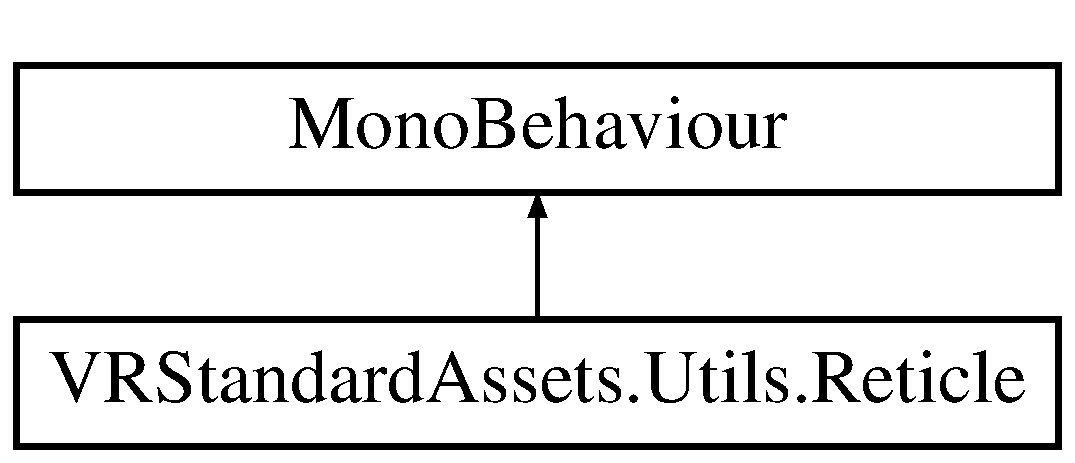
\includegraphics[height=2.000000cm]{class_v_r_standard_assets_1_1_utils_1_1_reticle}
\end{center}
\end{figure}
\subsection*{Public Member Functions}
\begin{DoxyCompactItemize}
\item 
void \mbox{\hyperlink{class_v_r_standard_assets_1_1_utils_1_1_reticle_aa738a82afd13d985233a21a0a74d9a33}{Hide}} ()
\item 
void \mbox{\hyperlink{class_v_r_standard_assets_1_1_utils_1_1_reticle_a29e671e0fa5061ea81bf3284a4093425}{Show}} ()
\item 
void \mbox{\hyperlink{class_v_r_standard_assets_1_1_utils_1_1_reticle_a3a2af7d74e5abbe61c4887a3c0e780dc}{Set\+Position}} (Vector3 position, Vector3 forward)
\item 
void \mbox{\hyperlink{class_v_r_standard_assets_1_1_utils_1_1_reticle_a7ab77d5bda342a42ad6ae65d8e157b25}{Set\+Position}} (Raycast\+Hit hit)
\end{DoxyCompactItemize}
\subsection*{Properties}
\begin{DoxyCompactItemize}
\item 
bool \mbox{\hyperlink{class_v_r_standard_assets_1_1_utils_1_1_reticle_a2a5bc273fd1f887161d635873b1bfca8}{Use\+Normal}}\hspace{0.3cm}{\ttfamily  \mbox{[}get, set\mbox{]}}
\item 
Transform \mbox{\hyperlink{class_v_r_standard_assets_1_1_utils_1_1_reticle_a1e6b411d542e1aa2f8891d97889c8a1c}{Reticle\+Transform}}\hspace{0.3cm}{\ttfamily  \mbox{[}get\mbox{]}}
\end{DoxyCompactItemize}
\subsection*{Private Member Functions}
\begin{DoxyCompactItemize}
\item 
void \mbox{\hyperlink{class_v_r_standard_assets_1_1_utils_1_1_reticle_ac8625110c11352313c81fb865a381c6b}{Awake}} ()
\end{DoxyCompactItemize}
\subsection*{Private Attributes}
\begin{DoxyCompactItemize}
\item 
float \mbox{\hyperlink{class_v_r_standard_assets_1_1_utils_1_1_reticle_ac77dc69ef46137708384c0cf3c0b3e28}{m\+\_\+\+Default\+Distance}} = 5f
\item 
bool \mbox{\hyperlink{class_v_r_standard_assets_1_1_utils_1_1_reticle_a8b0bdbc4b1b890400f1f6a36159eb05f}{m\+\_\+\+Use\+Normal}}
\item 
Image \mbox{\hyperlink{class_v_r_standard_assets_1_1_utils_1_1_reticle_a4153bcdb74fe1d18159d7c4608aa7bcf}{m\+\_\+\+Image}}
\item 
Transform \mbox{\hyperlink{class_v_r_standard_assets_1_1_utils_1_1_reticle_a16294edfd06ba0ec0d5d9d08caddf836}{m\+\_\+\+Reticle\+Transform}}
\item 
Transform \mbox{\hyperlink{class_v_r_standard_assets_1_1_utils_1_1_reticle_a741381fcd055dcd8be14a69f885e9a51}{m\+\_\+\+Camera}}
\item 
Vector3 \mbox{\hyperlink{class_v_r_standard_assets_1_1_utils_1_1_reticle_a58ca79ce295ea776a373e037dc8564cb}{m\+\_\+\+Original\+Scale}}
\item 
Quaternion \mbox{\hyperlink{class_v_r_standard_assets_1_1_utils_1_1_reticle_a79d3e7b210157509e2885c4152a8c717}{m\+\_\+\+Original\+Rotation}}
\end{DoxyCompactItemize}


\subsection{Member Function Documentation}
\mbox{\Hypertarget{class_v_r_standard_assets_1_1_utils_1_1_reticle_ac8625110c11352313c81fb865a381c6b}\label{class_v_r_standard_assets_1_1_utils_1_1_reticle_ac8625110c11352313c81fb865a381c6b}} 
\index{V\+R\+Standard\+Assets\+::\+Utils\+::\+Reticle@{V\+R\+Standard\+Assets\+::\+Utils\+::\+Reticle}!Awake@{Awake}}
\index{Awake@{Awake}!V\+R\+Standard\+Assets\+::\+Utils\+::\+Reticle@{V\+R\+Standard\+Assets\+::\+Utils\+::\+Reticle}}
\subsubsection{\texorpdfstring{Awake()}{Awake()}}
{\footnotesize\ttfamily void V\+R\+Standard\+Assets.\+Utils.\+Reticle.\+Awake (\begin{DoxyParamCaption}{ }\end{DoxyParamCaption})\hspace{0.3cm}{\ttfamily [private]}}

\mbox{\Hypertarget{class_v_r_standard_assets_1_1_utils_1_1_reticle_aa738a82afd13d985233a21a0a74d9a33}\label{class_v_r_standard_assets_1_1_utils_1_1_reticle_aa738a82afd13d985233a21a0a74d9a33}} 
\index{V\+R\+Standard\+Assets\+::\+Utils\+::\+Reticle@{V\+R\+Standard\+Assets\+::\+Utils\+::\+Reticle}!Hide@{Hide}}
\index{Hide@{Hide}!V\+R\+Standard\+Assets\+::\+Utils\+::\+Reticle@{V\+R\+Standard\+Assets\+::\+Utils\+::\+Reticle}}
\subsubsection{\texorpdfstring{Hide()}{Hide()}}
{\footnotesize\ttfamily void V\+R\+Standard\+Assets.\+Utils.\+Reticle.\+Hide (\begin{DoxyParamCaption}{ }\end{DoxyParamCaption})}

\mbox{\Hypertarget{class_v_r_standard_assets_1_1_utils_1_1_reticle_a3a2af7d74e5abbe61c4887a3c0e780dc}\label{class_v_r_standard_assets_1_1_utils_1_1_reticle_a3a2af7d74e5abbe61c4887a3c0e780dc}} 
\index{V\+R\+Standard\+Assets\+::\+Utils\+::\+Reticle@{V\+R\+Standard\+Assets\+::\+Utils\+::\+Reticle}!Set\+Position@{Set\+Position}}
\index{Set\+Position@{Set\+Position}!V\+R\+Standard\+Assets\+::\+Utils\+::\+Reticle@{V\+R\+Standard\+Assets\+::\+Utils\+::\+Reticle}}
\subsubsection{\texorpdfstring{Set\+Position()}{SetPosition()}\hspace{0.1cm}{\footnotesize\ttfamily [1/2]}}
{\footnotesize\ttfamily void V\+R\+Standard\+Assets.\+Utils.\+Reticle.\+Set\+Position (\begin{DoxyParamCaption}\item[{Vector3}]{position,  }\item[{Vector3}]{forward }\end{DoxyParamCaption})}

\mbox{\Hypertarget{class_v_r_standard_assets_1_1_utils_1_1_reticle_a7ab77d5bda342a42ad6ae65d8e157b25}\label{class_v_r_standard_assets_1_1_utils_1_1_reticle_a7ab77d5bda342a42ad6ae65d8e157b25}} 
\index{V\+R\+Standard\+Assets\+::\+Utils\+::\+Reticle@{V\+R\+Standard\+Assets\+::\+Utils\+::\+Reticle}!Set\+Position@{Set\+Position}}
\index{Set\+Position@{Set\+Position}!V\+R\+Standard\+Assets\+::\+Utils\+::\+Reticle@{V\+R\+Standard\+Assets\+::\+Utils\+::\+Reticle}}
\subsubsection{\texorpdfstring{Set\+Position()}{SetPosition()}\hspace{0.1cm}{\footnotesize\ttfamily [2/2]}}
{\footnotesize\ttfamily void V\+R\+Standard\+Assets.\+Utils.\+Reticle.\+Set\+Position (\begin{DoxyParamCaption}\item[{Raycast\+Hit}]{hit }\end{DoxyParamCaption})}

\mbox{\Hypertarget{class_v_r_standard_assets_1_1_utils_1_1_reticle_a29e671e0fa5061ea81bf3284a4093425}\label{class_v_r_standard_assets_1_1_utils_1_1_reticle_a29e671e0fa5061ea81bf3284a4093425}} 
\index{V\+R\+Standard\+Assets\+::\+Utils\+::\+Reticle@{V\+R\+Standard\+Assets\+::\+Utils\+::\+Reticle}!Show@{Show}}
\index{Show@{Show}!V\+R\+Standard\+Assets\+::\+Utils\+::\+Reticle@{V\+R\+Standard\+Assets\+::\+Utils\+::\+Reticle}}
\subsubsection{\texorpdfstring{Show()}{Show()}}
{\footnotesize\ttfamily void V\+R\+Standard\+Assets.\+Utils.\+Reticle.\+Show (\begin{DoxyParamCaption}{ }\end{DoxyParamCaption})}



\subsection{Member Data Documentation}
\mbox{\Hypertarget{class_v_r_standard_assets_1_1_utils_1_1_reticle_a741381fcd055dcd8be14a69f885e9a51}\label{class_v_r_standard_assets_1_1_utils_1_1_reticle_a741381fcd055dcd8be14a69f885e9a51}} 
\index{V\+R\+Standard\+Assets\+::\+Utils\+::\+Reticle@{V\+R\+Standard\+Assets\+::\+Utils\+::\+Reticle}!m\+\_\+\+Camera@{m\+\_\+\+Camera}}
\index{m\+\_\+\+Camera@{m\+\_\+\+Camera}!V\+R\+Standard\+Assets\+::\+Utils\+::\+Reticle@{V\+R\+Standard\+Assets\+::\+Utils\+::\+Reticle}}
\subsubsection{\texorpdfstring{m\+\_\+\+Camera}{m\_Camera}}
{\footnotesize\ttfamily Transform V\+R\+Standard\+Assets.\+Utils.\+Reticle.\+m\+\_\+\+Camera\hspace{0.3cm}{\ttfamily [private]}}

\mbox{\Hypertarget{class_v_r_standard_assets_1_1_utils_1_1_reticle_ac77dc69ef46137708384c0cf3c0b3e28}\label{class_v_r_standard_assets_1_1_utils_1_1_reticle_ac77dc69ef46137708384c0cf3c0b3e28}} 
\index{V\+R\+Standard\+Assets\+::\+Utils\+::\+Reticle@{V\+R\+Standard\+Assets\+::\+Utils\+::\+Reticle}!m\+\_\+\+Default\+Distance@{m\+\_\+\+Default\+Distance}}
\index{m\+\_\+\+Default\+Distance@{m\+\_\+\+Default\+Distance}!V\+R\+Standard\+Assets\+::\+Utils\+::\+Reticle@{V\+R\+Standard\+Assets\+::\+Utils\+::\+Reticle}}
\subsubsection{\texorpdfstring{m\+\_\+\+Default\+Distance}{m\_DefaultDistance}}
{\footnotesize\ttfamily float V\+R\+Standard\+Assets.\+Utils.\+Reticle.\+m\+\_\+\+Default\+Distance = 5f\hspace{0.3cm}{\ttfamily [private]}}

\mbox{\Hypertarget{class_v_r_standard_assets_1_1_utils_1_1_reticle_a4153bcdb74fe1d18159d7c4608aa7bcf}\label{class_v_r_standard_assets_1_1_utils_1_1_reticle_a4153bcdb74fe1d18159d7c4608aa7bcf}} 
\index{V\+R\+Standard\+Assets\+::\+Utils\+::\+Reticle@{V\+R\+Standard\+Assets\+::\+Utils\+::\+Reticle}!m\+\_\+\+Image@{m\+\_\+\+Image}}
\index{m\+\_\+\+Image@{m\+\_\+\+Image}!V\+R\+Standard\+Assets\+::\+Utils\+::\+Reticle@{V\+R\+Standard\+Assets\+::\+Utils\+::\+Reticle}}
\subsubsection{\texorpdfstring{m\+\_\+\+Image}{m\_Image}}
{\footnotesize\ttfamily Image V\+R\+Standard\+Assets.\+Utils.\+Reticle.\+m\+\_\+\+Image\hspace{0.3cm}{\ttfamily [private]}}

\mbox{\Hypertarget{class_v_r_standard_assets_1_1_utils_1_1_reticle_a79d3e7b210157509e2885c4152a8c717}\label{class_v_r_standard_assets_1_1_utils_1_1_reticle_a79d3e7b210157509e2885c4152a8c717}} 
\index{V\+R\+Standard\+Assets\+::\+Utils\+::\+Reticle@{V\+R\+Standard\+Assets\+::\+Utils\+::\+Reticle}!m\+\_\+\+Original\+Rotation@{m\+\_\+\+Original\+Rotation}}
\index{m\+\_\+\+Original\+Rotation@{m\+\_\+\+Original\+Rotation}!V\+R\+Standard\+Assets\+::\+Utils\+::\+Reticle@{V\+R\+Standard\+Assets\+::\+Utils\+::\+Reticle}}
\subsubsection{\texorpdfstring{m\+\_\+\+Original\+Rotation}{m\_OriginalRotation}}
{\footnotesize\ttfamily Quaternion V\+R\+Standard\+Assets.\+Utils.\+Reticle.\+m\+\_\+\+Original\+Rotation\hspace{0.3cm}{\ttfamily [private]}}

\mbox{\Hypertarget{class_v_r_standard_assets_1_1_utils_1_1_reticle_a58ca79ce295ea776a373e037dc8564cb}\label{class_v_r_standard_assets_1_1_utils_1_1_reticle_a58ca79ce295ea776a373e037dc8564cb}} 
\index{V\+R\+Standard\+Assets\+::\+Utils\+::\+Reticle@{V\+R\+Standard\+Assets\+::\+Utils\+::\+Reticle}!m\+\_\+\+Original\+Scale@{m\+\_\+\+Original\+Scale}}
\index{m\+\_\+\+Original\+Scale@{m\+\_\+\+Original\+Scale}!V\+R\+Standard\+Assets\+::\+Utils\+::\+Reticle@{V\+R\+Standard\+Assets\+::\+Utils\+::\+Reticle}}
\subsubsection{\texorpdfstring{m\+\_\+\+Original\+Scale}{m\_OriginalScale}}
{\footnotesize\ttfamily Vector3 V\+R\+Standard\+Assets.\+Utils.\+Reticle.\+m\+\_\+\+Original\+Scale\hspace{0.3cm}{\ttfamily [private]}}

\mbox{\Hypertarget{class_v_r_standard_assets_1_1_utils_1_1_reticle_a16294edfd06ba0ec0d5d9d08caddf836}\label{class_v_r_standard_assets_1_1_utils_1_1_reticle_a16294edfd06ba0ec0d5d9d08caddf836}} 
\index{V\+R\+Standard\+Assets\+::\+Utils\+::\+Reticle@{V\+R\+Standard\+Assets\+::\+Utils\+::\+Reticle}!m\+\_\+\+Reticle\+Transform@{m\+\_\+\+Reticle\+Transform}}
\index{m\+\_\+\+Reticle\+Transform@{m\+\_\+\+Reticle\+Transform}!V\+R\+Standard\+Assets\+::\+Utils\+::\+Reticle@{V\+R\+Standard\+Assets\+::\+Utils\+::\+Reticle}}
\subsubsection{\texorpdfstring{m\+\_\+\+Reticle\+Transform}{m\_ReticleTransform}}
{\footnotesize\ttfamily Transform V\+R\+Standard\+Assets.\+Utils.\+Reticle.\+m\+\_\+\+Reticle\+Transform\hspace{0.3cm}{\ttfamily [private]}}

\mbox{\Hypertarget{class_v_r_standard_assets_1_1_utils_1_1_reticle_a8b0bdbc4b1b890400f1f6a36159eb05f}\label{class_v_r_standard_assets_1_1_utils_1_1_reticle_a8b0bdbc4b1b890400f1f6a36159eb05f}} 
\index{V\+R\+Standard\+Assets\+::\+Utils\+::\+Reticle@{V\+R\+Standard\+Assets\+::\+Utils\+::\+Reticle}!m\+\_\+\+Use\+Normal@{m\+\_\+\+Use\+Normal}}
\index{m\+\_\+\+Use\+Normal@{m\+\_\+\+Use\+Normal}!V\+R\+Standard\+Assets\+::\+Utils\+::\+Reticle@{V\+R\+Standard\+Assets\+::\+Utils\+::\+Reticle}}
\subsubsection{\texorpdfstring{m\+\_\+\+Use\+Normal}{m\_UseNormal}}
{\footnotesize\ttfamily bool V\+R\+Standard\+Assets.\+Utils.\+Reticle.\+m\+\_\+\+Use\+Normal\hspace{0.3cm}{\ttfamily [private]}}



\subsection{Property Documentation}
\mbox{\Hypertarget{class_v_r_standard_assets_1_1_utils_1_1_reticle_a1e6b411d542e1aa2f8891d97889c8a1c}\label{class_v_r_standard_assets_1_1_utils_1_1_reticle_a1e6b411d542e1aa2f8891d97889c8a1c}} 
\index{V\+R\+Standard\+Assets\+::\+Utils\+::\+Reticle@{V\+R\+Standard\+Assets\+::\+Utils\+::\+Reticle}!Reticle\+Transform@{Reticle\+Transform}}
\index{Reticle\+Transform@{Reticle\+Transform}!V\+R\+Standard\+Assets\+::\+Utils\+::\+Reticle@{V\+R\+Standard\+Assets\+::\+Utils\+::\+Reticle}}
\subsubsection{\texorpdfstring{Reticle\+Transform}{ReticleTransform}}
{\footnotesize\ttfamily Transform V\+R\+Standard\+Assets.\+Utils.\+Reticle.\+Reticle\+Transform\hspace{0.3cm}{\ttfamily [get]}}

\mbox{\Hypertarget{class_v_r_standard_assets_1_1_utils_1_1_reticle_a2a5bc273fd1f887161d635873b1bfca8}\label{class_v_r_standard_assets_1_1_utils_1_1_reticle_a2a5bc273fd1f887161d635873b1bfca8}} 
\index{V\+R\+Standard\+Assets\+::\+Utils\+::\+Reticle@{V\+R\+Standard\+Assets\+::\+Utils\+::\+Reticle}!Use\+Normal@{Use\+Normal}}
\index{Use\+Normal@{Use\+Normal}!V\+R\+Standard\+Assets\+::\+Utils\+::\+Reticle@{V\+R\+Standard\+Assets\+::\+Utils\+::\+Reticle}}
\subsubsection{\texorpdfstring{Use\+Normal}{UseNormal}}
{\footnotesize\ttfamily bool V\+R\+Standard\+Assets.\+Utils.\+Reticle.\+Use\+Normal\hspace{0.3cm}{\ttfamily [get]}, {\ttfamily [set]}}



The documentation for this class was generated from the following file\+:\begin{DoxyCompactItemize}
\item 
\mbox{\hyperlink{_reticle_8cs}{Reticle.\+cs}}\end{DoxyCompactItemize}

\hypertarget{class_stage1}{}\section{Stage1 Class Reference}
\label{class_stage1}\index{Stage1@{Stage1}}
Inheritance diagram for Stage1\+:\begin{figure}[H]
\begin{center}
\leavevmode
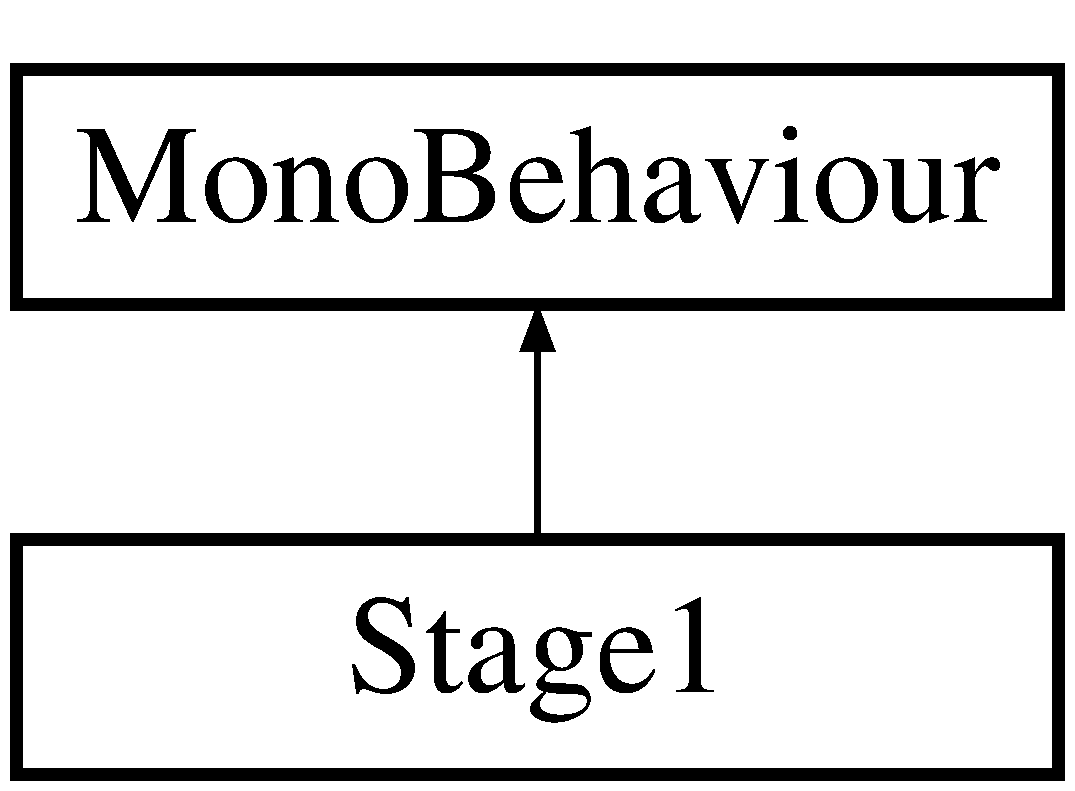
\includegraphics[height=2.000000cm]{class_stage1}
\end{center}
\end{figure}
\subsection*{Static Public Attributes}
\begin{DoxyCompactItemize}
\item 
static \mbox{\hyperlink{class_stage1}{Stage1}} \mbox{\hyperlink{class_stage1_ab20fb1804b3c34a0d5f0df630b79f48c}{s\+\_\+\+Instance}}
\end{DoxyCompactItemize}
\subsection*{Private Member Functions}
\begin{DoxyCompactItemize}
\item 
void \mbox{\hyperlink{class_stage1_a22cb4953258834766118cccf6637bf6e}{Start}} ()
\item 
void \mbox{\hyperlink{class_stage1_a31a6ea5ef3ab028a99be7116cd90e37f}{Update}} ()
\item 
void \mbox{\hyperlink{class_stage1_aa992bad0fdb8df10f5ea6689ef8863ae}{Register\+Arrow}} ()
\begin{DoxyCompactList}\small\item\em Registers the arrow as successfully looked at and increments {\ttfamily i\+\_\+\+Current\+Arrow} \end{DoxyCompactList}\item 
void \mbox{\hyperlink{class_stage1_ac86ffd4a366e400042b42869b9282594}{Reset\+Progress\+Bar}} ()
\begin{DoxyCompactList}\small\item\em Resets the progress bar back to 0. \end{DoxyCompactList}\item 
void \mbox{\hyperlink{class_stage1_af625f5fcec1c9ac7a6fd6d74e437c13e}{Load\+Progress\+Bar}} ()
\begin{DoxyCompactList}\small\item\em Precondition\+: Expecting to be called in Update. Loads the progress bar by one step. \end{DoxyCompactList}\item 
void \mbox{\hyperlink{class_stage1_a6792b3b46499c0c5a6bf63031f6783b7}{Face\+Arrows\+To\+User}} ()
\begin{DoxyCompactList}\small\item\em Iterates through the arrows and makes them face the user \end{DoxyCompactList}\end{DoxyCompactItemize}
\subsection*{Private Attributes}
\begin{DoxyCompactItemize}
\item 
\mbox{\hyperlink{class_v_r_standard_assets_1_1_utils_1_1_raycaster_v_r}{Raycaster\+VR}} \mbox{\hyperlink{class_stage1_a8df5a3c960c460aed5d994cc74598294}{m\+\_\+\+Raycaster\+Script}}
\item 
\mbox{\hyperlink{class_intro_session_manager}{Intro\+Session\+Manager}} \mbox{\hyperlink{class_stage1_aa75e5070f730ce1c8a22374540b5a165}{m\+\_\+\+Manager}}
\item 
\mbox{\hyperlink{class_dialogue}{Dialogue}} \mbox{\hyperlink{class_stage1_a5e0b22e242f1dc57f25116368047a74a}{m\+\_\+\+Dialogue\+Instructions}}
\item 
\mbox{\hyperlink{class_dialogue}{Dialogue}} \mbox{\hyperlink{class_stage1_a053a8aac4bdbe9827e07d00b10c89ddb}{m\+\_\+\+Dialogue\+Fail}}
\item 
Game\+Object \mbox{[}$\,$\mbox{]} \mbox{\hyperlink{class_stage1_a61cc42d02ddfdb4c9e2deb58783a2106}{m\+\_\+\+Arrows\+Object\+List}} = new Game\+Object\mbox{[}4\mbox{]}
\item 
Transform \mbox{\hyperlink{class_stage1_a3833d350fc50f9ad32af955e6f2cdd7a}{m\+\_\+\+Center\+Position}}
\item 
float \mbox{\hyperlink{class_stage1_a717cdee3689d0e77cefec54c8f0c6ca4}{m\+\_\+\+Progress\+Bar\+Load\+Time}} = 2f
\item 
float \mbox{\hyperlink{class_stage1_a25cdcb8d515ce432b7656735e6920559}{m\+\_\+\+Loaded}} = 0
\item 
float \mbox{\hyperlink{class_stage1_a6d69553223e46e861ace3e060792508f}{m\+\_\+\+Reticle\+Scale\+Factor}}
\item 
Image \mbox{\hyperlink{class_stage1_a3bf55a6567f3517d9882c4c5e75b9864}{m\+\_\+\+Loading\+Bar}}
\item 
string \mbox{[}$\,$\mbox{]} \mbox{\hyperlink{class_stage1_a19950f79b749e93f7588fe8f2b4c41f4}{m\+\_\+\+Arrows\+List}}
\item 
int \mbox{\hyperlink{class_stage1_a1c91dd1b16a5f371f684ef8c9f8c28b6}{i\+\_\+\+Current\+Arrow}}
\item 
Game\+Object \mbox{\hyperlink{class_stage1_ab34fda2e3ccabd8793c8749951277a6b}{m\+\_\+\+Target}}
\item 
bool \mbox{\hyperlink{class_stage1_a0388f6c2c86f10d5490731d6ba84be39}{m\+\_\+\+Was\+Looking\+At\+Arrow}}
\item 
bool \mbox{\hyperlink{class_stage1_ac4aaa3ab55eca6e4e561a51c7257d246}{m\+\_\+\+Is\+Stage\+Complete}}
\item 
Hashtable \mbox{\hyperlink{class_stage1_a013cab53ec598101d39197f1eae83e44}{m\+\_\+\+Arrow\+Map}}
\item 
bool \mbox{\hyperlink{class_stage1_ae2f93b4706065e7891ece3becaeef9cd}{m\+\_\+\+Looking\+At\+Completed}}
\item 
Game\+Object \mbox{\hyperlink{class_stage1_a6ffff0ae9f4d8ba81069bbec5fa8b899}{m\+\_\+\+Reticle}}
\item 
Game\+Object \mbox{\hyperlink{class_stage1_a61914e3464e7a11b41cdf5fb2516a619}{m\+\_\+\+Center\+Eye\+Anchor}}
\end{DoxyCompactItemize}


\subsection{Member Function Documentation}
\mbox{\Hypertarget{class_stage1_a6792b3b46499c0c5a6bf63031f6783b7}\label{class_stage1_a6792b3b46499c0c5a6bf63031f6783b7}} 
\index{Stage1@{Stage1}!Face\+Arrows\+To\+User@{Face\+Arrows\+To\+User}}
\index{Face\+Arrows\+To\+User@{Face\+Arrows\+To\+User}!Stage1@{Stage1}}
\subsubsection{\texorpdfstring{Face\+Arrows\+To\+User()}{FaceArrowsToUser()}}
{\footnotesize\ttfamily void Stage1.\+Face\+Arrows\+To\+User (\begin{DoxyParamCaption}{ }\end{DoxyParamCaption})\hspace{0.3cm}{\ttfamily [private]}}



Iterates through the arrows and makes them face the user 

\mbox{\Hypertarget{class_stage1_af625f5fcec1c9ac7a6fd6d74e437c13e}\label{class_stage1_af625f5fcec1c9ac7a6fd6d74e437c13e}} 
\index{Stage1@{Stage1}!Load\+Progress\+Bar@{Load\+Progress\+Bar}}
\index{Load\+Progress\+Bar@{Load\+Progress\+Bar}!Stage1@{Stage1}}
\subsubsection{\texorpdfstring{Load\+Progress\+Bar()}{LoadProgressBar()}}
{\footnotesize\ttfamily void Stage1.\+Load\+Progress\+Bar (\begin{DoxyParamCaption}{ }\end{DoxyParamCaption})\hspace{0.3cm}{\ttfamily [private]}}



Precondition\+: Expecting to be called in Update. Loads the progress bar by one step. 

\mbox{\Hypertarget{class_stage1_aa992bad0fdb8df10f5ea6689ef8863ae}\label{class_stage1_aa992bad0fdb8df10f5ea6689ef8863ae}} 
\index{Stage1@{Stage1}!Register\+Arrow@{Register\+Arrow}}
\index{Register\+Arrow@{Register\+Arrow}!Stage1@{Stage1}}
\subsubsection{\texorpdfstring{Register\+Arrow()}{RegisterArrow()}}
{\footnotesize\ttfamily void Stage1.\+Register\+Arrow (\begin{DoxyParamCaption}{ }\end{DoxyParamCaption})\hspace{0.3cm}{\ttfamily [private]}}



Registers the arrow as successfully looked at and increments {\ttfamily i\+\_\+\+Current\+Arrow} 

\mbox{\Hypertarget{class_stage1_ac86ffd4a366e400042b42869b9282594}\label{class_stage1_ac86ffd4a366e400042b42869b9282594}} 
\index{Stage1@{Stage1}!Reset\+Progress\+Bar@{Reset\+Progress\+Bar}}
\index{Reset\+Progress\+Bar@{Reset\+Progress\+Bar}!Stage1@{Stage1}}
\subsubsection{\texorpdfstring{Reset\+Progress\+Bar()}{ResetProgressBar()}}
{\footnotesize\ttfamily void Stage1.\+Reset\+Progress\+Bar (\begin{DoxyParamCaption}{ }\end{DoxyParamCaption})\hspace{0.3cm}{\ttfamily [private]}}



Resets the progress bar back to 0. 

\mbox{\Hypertarget{class_stage1_a22cb4953258834766118cccf6637bf6e}\label{class_stage1_a22cb4953258834766118cccf6637bf6e}} 
\index{Stage1@{Stage1}!Start@{Start}}
\index{Start@{Start}!Stage1@{Stage1}}
\subsubsection{\texorpdfstring{Start()}{Start()}}
{\footnotesize\ttfamily void Stage1.\+Start (\begin{DoxyParamCaption}{ }\end{DoxyParamCaption})\hspace{0.3cm}{\ttfamily [private]}}

\mbox{\Hypertarget{class_stage1_a31a6ea5ef3ab028a99be7116cd90e37f}\label{class_stage1_a31a6ea5ef3ab028a99be7116cd90e37f}} 
\index{Stage1@{Stage1}!Update@{Update}}
\index{Update@{Update}!Stage1@{Stage1}}
\subsubsection{\texorpdfstring{Update()}{Update()}}
{\footnotesize\ttfamily void Stage1.\+Update (\begin{DoxyParamCaption}{ }\end{DoxyParamCaption})\hspace{0.3cm}{\ttfamily [private]}}



\subsection{Member Data Documentation}
\mbox{\Hypertarget{class_stage1_a1c91dd1b16a5f371f684ef8c9f8c28b6}\label{class_stage1_a1c91dd1b16a5f371f684ef8c9f8c28b6}} 
\index{Stage1@{Stage1}!i\+\_\+\+Current\+Arrow@{i\+\_\+\+Current\+Arrow}}
\index{i\+\_\+\+Current\+Arrow@{i\+\_\+\+Current\+Arrow}!Stage1@{Stage1}}
\subsubsection{\texorpdfstring{i\+\_\+\+Current\+Arrow}{i\_CurrentArrow}}
{\footnotesize\ttfamily int Stage1.\+i\+\_\+\+Current\+Arrow\hspace{0.3cm}{\ttfamily [private]}}

\mbox{\Hypertarget{class_stage1_a013cab53ec598101d39197f1eae83e44}\label{class_stage1_a013cab53ec598101d39197f1eae83e44}} 
\index{Stage1@{Stage1}!m\+\_\+\+Arrow\+Map@{m\+\_\+\+Arrow\+Map}}
\index{m\+\_\+\+Arrow\+Map@{m\+\_\+\+Arrow\+Map}!Stage1@{Stage1}}
\subsubsection{\texorpdfstring{m\+\_\+\+Arrow\+Map}{m\_ArrowMap}}
{\footnotesize\ttfamily Hashtable Stage1.\+m\+\_\+\+Arrow\+Map\hspace{0.3cm}{\ttfamily [private]}}

\mbox{\Hypertarget{class_stage1_a19950f79b749e93f7588fe8f2b4c41f4}\label{class_stage1_a19950f79b749e93f7588fe8f2b4c41f4}} 
\index{Stage1@{Stage1}!m\+\_\+\+Arrows\+List@{m\+\_\+\+Arrows\+List}}
\index{m\+\_\+\+Arrows\+List@{m\+\_\+\+Arrows\+List}!Stage1@{Stage1}}
\subsubsection{\texorpdfstring{m\+\_\+\+Arrows\+List}{m\_ArrowsList}}
{\footnotesize\ttfamily string \mbox{[}$\,$\mbox{]} Stage1.\+m\+\_\+\+Arrows\+List\hspace{0.3cm}{\ttfamily [private]}}

\mbox{\Hypertarget{class_stage1_a61cc42d02ddfdb4c9e2deb58783a2106}\label{class_stage1_a61cc42d02ddfdb4c9e2deb58783a2106}} 
\index{Stage1@{Stage1}!m\+\_\+\+Arrows\+Object\+List@{m\+\_\+\+Arrows\+Object\+List}}
\index{m\+\_\+\+Arrows\+Object\+List@{m\+\_\+\+Arrows\+Object\+List}!Stage1@{Stage1}}
\subsubsection{\texorpdfstring{m\+\_\+\+Arrows\+Object\+List}{m\_ArrowsObjectList}}
{\footnotesize\ttfamily Game\+Object \mbox{[}$\,$\mbox{]} Stage1.\+m\+\_\+\+Arrows\+Object\+List = new Game\+Object\mbox{[}4\mbox{]}\hspace{0.3cm}{\ttfamily [private]}}

\mbox{\Hypertarget{class_stage1_a61914e3464e7a11b41cdf5fb2516a619}\label{class_stage1_a61914e3464e7a11b41cdf5fb2516a619}} 
\index{Stage1@{Stage1}!m\+\_\+\+Center\+Eye\+Anchor@{m\+\_\+\+Center\+Eye\+Anchor}}
\index{m\+\_\+\+Center\+Eye\+Anchor@{m\+\_\+\+Center\+Eye\+Anchor}!Stage1@{Stage1}}
\subsubsection{\texorpdfstring{m\+\_\+\+Center\+Eye\+Anchor}{m\_CenterEyeAnchor}}
{\footnotesize\ttfamily Game\+Object Stage1.\+m\+\_\+\+Center\+Eye\+Anchor\hspace{0.3cm}{\ttfamily [private]}}

\mbox{\Hypertarget{class_stage1_a3833d350fc50f9ad32af955e6f2cdd7a}\label{class_stage1_a3833d350fc50f9ad32af955e6f2cdd7a}} 
\index{Stage1@{Stage1}!m\+\_\+\+Center\+Position@{m\+\_\+\+Center\+Position}}
\index{m\+\_\+\+Center\+Position@{m\+\_\+\+Center\+Position}!Stage1@{Stage1}}
\subsubsection{\texorpdfstring{m\+\_\+\+Center\+Position}{m\_CenterPosition}}
{\footnotesize\ttfamily Transform Stage1.\+m\+\_\+\+Center\+Position\hspace{0.3cm}{\ttfamily [private]}}

\mbox{\Hypertarget{class_stage1_a053a8aac4bdbe9827e07d00b10c89ddb}\label{class_stage1_a053a8aac4bdbe9827e07d00b10c89ddb}} 
\index{Stage1@{Stage1}!m\+\_\+\+Dialogue\+Fail@{m\+\_\+\+Dialogue\+Fail}}
\index{m\+\_\+\+Dialogue\+Fail@{m\+\_\+\+Dialogue\+Fail}!Stage1@{Stage1}}
\subsubsection{\texorpdfstring{m\+\_\+\+Dialogue\+Fail}{m\_DialogueFail}}
{\footnotesize\ttfamily \mbox{\hyperlink{class_dialogue}{Dialogue}} Stage1.\+m\+\_\+\+Dialogue\+Fail\hspace{0.3cm}{\ttfamily [private]}}

\mbox{\Hypertarget{class_stage1_a5e0b22e242f1dc57f25116368047a74a}\label{class_stage1_a5e0b22e242f1dc57f25116368047a74a}} 
\index{Stage1@{Stage1}!m\+\_\+\+Dialogue\+Instructions@{m\+\_\+\+Dialogue\+Instructions}}
\index{m\+\_\+\+Dialogue\+Instructions@{m\+\_\+\+Dialogue\+Instructions}!Stage1@{Stage1}}
\subsubsection{\texorpdfstring{m\+\_\+\+Dialogue\+Instructions}{m\_DialogueInstructions}}
{\footnotesize\ttfamily \mbox{\hyperlink{class_dialogue}{Dialogue}} Stage1.\+m\+\_\+\+Dialogue\+Instructions\hspace{0.3cm}{\ttfamily [private]}}

\mbox{\Hypertarget{class_stage1_ac4aaa3ab55eca6e4e561a51c7257d246}\label{class_stage1_ac4aaa3ab55eca6e4e561a51c7257d246}} 
\index{Stage1@{Stage1}!m\+\_\+\+Is\+Stage\+Complete@{m\+\_\+\+Is\+Stage\+Complete}}
\index{m\+\_\+\+Is\+Stage\+Complete@{m\+\_\+\+Is\+Stage\+Complete}!Stage1@{Stage1}}
\subsubsection{\texorpdfstring{m\+\_\+\+Is\+Stage\+Complete}{m\_IsStageComplete}}
{\footnotesize\ttfamily bool Stage1.\+m\+\_\+\+Is\+Stage\+Complete\hspace{0.3cm}{\ttfamily [private]}}

\mbox{\Hypertarget{class_stage1_a25cdcb8d515ce432b7656735e6920559}\label{class_stage1_a25cdcb8d515ce432b7656735e6920559}} 
\index{Stage1@{Stage1}!m\+\_\+\+Loaded@{m\+\_\+\+Loaded}}
\index{m\+\_\+\+Loaded@{m\+\_\+\+Loaded}!Stage1@{Stage1}}
\subsubsection{\texorpdfstring{m\+\_\+\+Loaded}{m\_Loaded}}
{\footnotesize\ttfamily float Stage1.\+m\+\_\+\+Loaded = 0\hspace{0.3cm}{\ttfamily [private]}}

\mbox{\Hypertarget{class_stage1_a3bf55a6567f3517d9882c4c5e75b9864}\label{class_stage1_a3bf55a6567f3517d9882c4c5e75b9864}} 
\index{Stage1@{Stage1}!m\+\_\+\+Loading\+Bar@{m\+\_\+\+Loading\+Bar}}
\index{m\+\_\+\+Loading\+Bar@{m\+\_\+\+Loading\+Bar}!Stage1@{Stage1}}
\subsubsection{\texorpdfstring{m\+\_\+\+Loading\+Bar}{m\_LoadingBar}}
{\footnotesize\ttfamily Image Stage1.\+m\+\_\+\+Loading\+Bar\hspace{0.3cm}{\ttfamily [private]}}

\mbox{\Hypertarget{class_stage1_ae2f93b4706065e7891ece3becaeef9cd}\label{class_stage1_ae2f93b4706065e7891ece3becaeef9cd}} 
\index{Stage1@{Stage1}!m\+\_\+\+Looking\+At\+Completed@{m\+\_\+\+Looking\+At\+Completed}}
\index{m\+\_\+\+Looking\+At\+Completed@{m\+\_\+\+Looking\+At\+Completed}!Stage1@{Stage1}}
\subsubsection{\texorpdfstring{m\+\_\+\+Looking\+At\+Completed}{m\_LookingAtCompleted}}
{\footnotesize\ttfamily bool Stage1.\+m\+\_\+\+Looking\+At\+Completed\hspace{0.3cm}{\ttfamily [private]}}

\mbox{\Hypertarget{class_stage1_aa75e5070f730ce1c8a22374540b5a165}\label{class_stage1_aa75e5070f730ce1c8a22374540b5a165}} 
\index{Stage1@{Stage1}!m\+\_\+\+Manager@{m\+\_\+\+Manager}}
\index{m\+\_\+\+Manager@{m\+\_\+\+Manager}!Stage1@{Stage1}}
\subsubsection{\texorpdfstring{m\+\_\+\+Manager}{m\_Manager}}
{\footnotesize\ttfamily \mbox{\hyperlink{class_intro_session_manager}{Intro\+Session\+Manager}} Stage1.\+m\+\_\+\+Manager\hspace{0.3cm}{\ttfamily [private]}}

\mbox{\Hypertarget{class_stage1_a717cdee3689d0e77cefec54c8f0c6ca4}\label{class_stage1_a717cdee3689d0e77cefec54c8f0c6ca4}} 
\index{Stage1@{Stage1}!m\+\_\+\+Progress\+Bar\+Load\+Time@{m\+\_\+\+Progress\+Bar\+Load\+Time}}
\index{m\+\_\+\+Progress\+Bar\+Load\+Time@{m\+\_\+\+Progress\+Bar\+Load\+Time}!Stage1@{Stage1}}
\subsubsection{\texorpdfstring{m\+\_\+\+Progress\+Bar\+Load\+Time}{m\_ProgressBarLoadTime}}
{\footnotesize\ttfamily float Stage1.\+m\+\_\+\+Progress\+Bar\+Load\+Time = 2f\hspace{0.3cm}{\ttfamily [private]}}

\mbox{\Hypertarget{class_stage1_a8df5a3c960c460aed5d994cc74598294}\label{class_stage1_a8df5a3c960c460aed5d994cc74598294}} 
\index{Stage1@{Stage1}!m\+\_\+\+Raycaster\+Script@{m\+\_\+\+Raycaster\+Script}}
\index{m\+\_\+\+Raycaster\+Script@{m\+\_\+\+Raycaster\+Script}!Stage1@{Stage1}}
\subsubsection{\texorpdfstring{m\+\_\+\+Raycaster\+Script}{m\_RaycasterScript}}
{\footnotesize\ttfamily \mbox{\hyperlink{class_v_r_standard_assets_1_1_utils_1_1_raycaster_v_r}{Raycaster\+VR}} Stage1.\+m\+\_\+\+Raycaster\+Script\hspace{0.3cm}{\ttfamily [private]}}

\mbox{\Hypertarget{class_stage1_a6ffff0ae9f4d8ba81069bbec5fa8b899}\label{class_stage1_a6ffff0ae9f4d8ba81069bbec5fa8b899}} 
\index{Stage1@{Stage1}!m\+\_\+\+Reticle@{m\+\_\+\+Reticle}}
\index{m\+\_\+\+Reticle@{m\+\_\+\+Reticle}!Stage1@{Stage1}}
\subsubsection{\texorpdfstring{m\+\_\+\+Reticle}{m\_Reticle}}
{\footnotesize\ttfamily Game\+Object Stage1.\+m\+\_\+\+Reticle\hspace{0.3cm}{\ttfamily [private]}}

\mbox{\Hypertarget{class_stage1_a6d69553223e46e861ace3e060792508f}\label{class_stage1_a6d69553223e46e861ace3e060792508f}} 
\index{Stage1@{Stage1}!m\+\_\+\+Reticle\+Scale\+Factor@{m\+\_\+\+Reticle\+Scale\+Factor}}
\index{m\+\_\+\+Reticle\+Scale\+Factor@{m\+\_\+\+Reticle\+Scale\+Factor}!Stage1@{Stage1}}
\subsubsection{\texorpdfstring{m\+\_\+\+Reticle\+Scale\+Factor}{m\_ReticleScaleFactor}}
{\footnotesize\ttfamily float Stage1.\+m\+\_\+\+Reticle\+Scale\+Factor\hspace{0.3cm}{\ttfamily [private]}}

\mbox{\Hypertarget{class_stage1_ab34fda2e3ccabd8793c8749951277a6b}\label{class_stage1_ab34fda2e3ccabd8793c8749951277a6b}} 
\index{Stage1@{Stage1}!m\+\_\+\+Target@{m\+\_\+\+Target}}
\index{m\+\_\+\+Target@{m\+\_\+\+Target}!Stage1@{Stage1}}
\subsubsection{\texorpdfstring{m\+\_\+\+Target}{m\_Target}}
{\footnotesize\ttfamily Game\+Object Stage1.\+m\+\_\+\+Target\hspace{0.3cm}{\ttfamily [private]}}

\mbox{\Hypertarget{class_stage1_a0388f6c2c86f10d5490731d6ba84be39}\label{class_stage1_a0388f6c2c86f10d5490731d6ba84be39}} 
\index{Stage1@{Stage1}!m\+\_\+\+Was\+Looking\+At\+Arrow@{m\+\_\+\+Was\+Looking\+At\+Arrow}}
\index{m\+\_\+\+Was\+Looking\+At\+Arrow@{m\+\_\+\+Was\+Looking\+At\+Arrow}!Stage1@{Stage1}}
\subsubsection{\texorpdfstring{m\+\_\+\+Was\+Looking\+At\+Arrow}{m\_WasLookingAtArrow}}
{\footnotesize\ttfamily bool Stage1.\+m\+\_\+\+Was\+Looking\+At\+Arrow\hspace{0.3cm}{\ttfamily [private]}}

\mbox{\Hypertarget{class_stage1_ab20fb1804b3c34a0d5f0df630b79f48c}\label{class_stage1_ab20fb1804b3c34a0d5f0df630b79f48c}} 
\index{Stage1@{Stage1}!s\+\_\+\+Instance@{s\+\_\+\+Instance}}
\index{s\+\_\+\+Instance@{s\+\_\+\+Instance}!Stage1@{Stage1}}
\subsubsection{\texorpdfstring{s\+\_\+\+Instance}{s\_Instance}}
{\footnotesize\ttfamily \mbox{\hyperlink{class_stage1}{Stage1}} Stage1.\+s\+\_\+\+Instance\hspace{0.3cm}{\ttfamily [static]}}



The documentation for this class was generated from the following file\+:\begin{DoxyCompactItemize}
\item 
\mbox{\hyperlink{_stage1_8cs}{Stage1.\+cs}}\end{DoxyCompactItemize}

\hypertarget{class_stage2}{}\section{Stage2 Class Reference}
\label{class_stage2}\index{Stage2@{Stage2}}
Inheritance diagram for Stage2\+:\begin{figure}[H]
\begin{center}
\leavevmode
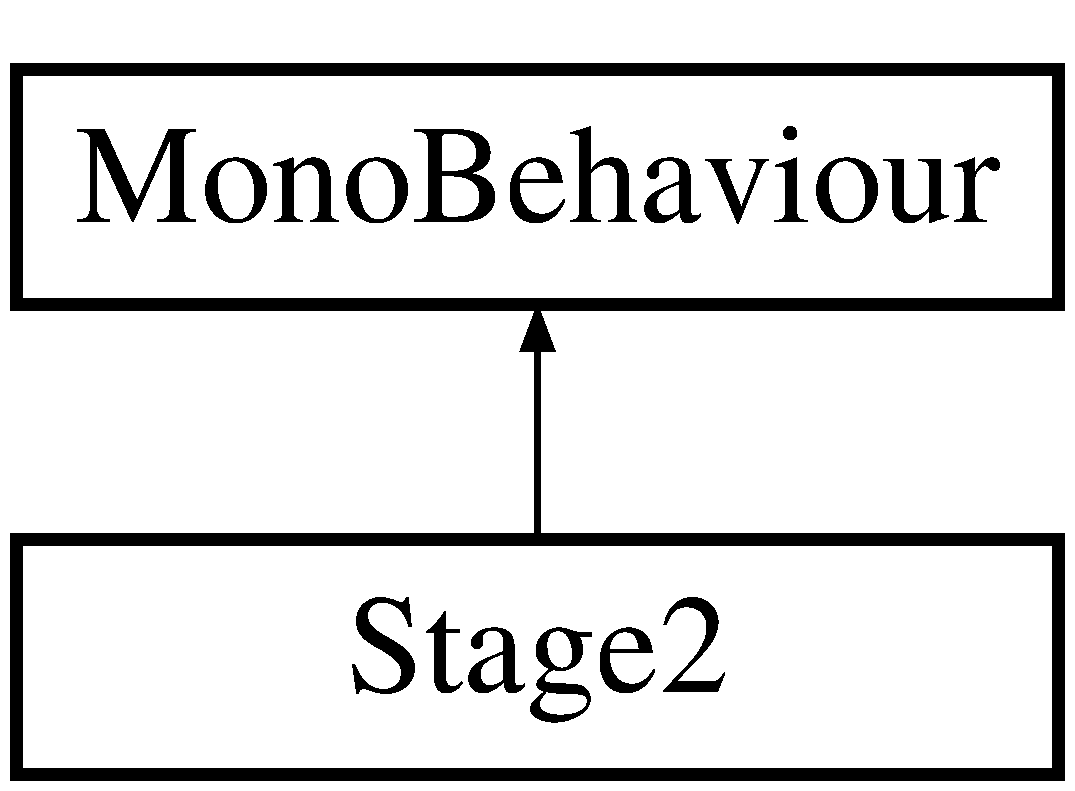
\includegraphics[height=2.000000cm]{class_stage2}
\end{center}
\end{figure}
\subsection*{Static Public Attributes}
\begin{DoxyCompactItemize}
\item 
static \mbox{\hyperlink{class_stage2}{Stage2}} \mbox{\hyperlink{class_stage2_ab0b9069fe51d69bfbe6b847dccd5dbd4}{s\+\_\+\+Instance}} = null
\end{DoxyCompactItemize}
\subsection*{Private Member Functions}
\begin{DoxyCompactItemize}
\item 
void \mbox{\hyperlink{class_stage2_a6ef397aad3d634caf09da4dc09dfeffa}{Start}} ()
\item 
void \mbox{\hyperlink{class_stage2_a50f93eb0e6e1ef6e71d85df9f951f189}{Update}} ()
\end{DoxyCompactItemize}
\subsection*{Private Attributes}
\begin{DoxyCompactItemize}
\item 
\mbox{\hyperlink{class_intro_session_manager}{Intro\+Session\+Manager}} \mbox{\hyperlink{class_stage2_ac0c7fd7470c7a7119e6990c794d4b6da}{m\+\_\+\+Manager}}
\item 
\mbox{\hyperlink{class_dialogue}{Dialogue}} \mbox{\hyperlink{class_stage2_a568227038f1502ead76a3063cb56e7ad}{m\+\_\+\+Dialogue\+Instructions}}
\item 
\mbox{\hyperlink{class_dialogue}{Dialogue}} \mbox{\hyperlink{class_stage2_a1976a81381663da59cdb6e16d2c303e4}{m\+\_\+\+Dialogue\+Fail}}
\item 
int \mbox{\hyperlink{class_stage2_a91dc2a2d19d9cecdf3faf0d63670570b}{i\+\_\+\+Error\+Counter}} = 0
\item 
int \mbox{\hyperlink{class_stage2_acfd2cec2899355884335066e879af778}{m\+\_\+\+Number\+Of\+Tries}} = 2
\item 
bool \mbox{\hyperlink{class_stage2_a7716d04bef0e8c283cdb51aa09d288da}{m\+\_\+\+Check\+Recenter}} = true
\item 
bool \mbox{\hyperlink{class_stage2_a1bf043d9a2be31a8be2000e3ac763a69}{m\+\_\+\+Intro\+Not\+Started}} = true
\end{DoxyCompactItemize}


\subsection{Member Function Documentation}
\mbox{\Hypertarget{class_stage2_a6ef397aad3d634caf09da4dc09dfeffa}\label{class_stage2_a6ef397aad3d634caf09da4dc09dfeffa}} 
\index{Stage2@{Stage2}!Start@{Start}}
\index{Start@{Start}!Stage2@{Stage2}}
\subsubsection{\texorpdfstring{Start()}{Start()}}
{\footnotesize\ttfamily void Stage2.\+Start (\begin{DoxyParamCaption}{ }\end{DoxyParamCaption})\hspace{0.3cm}{\ttfamily [private]}}

\mbox{\Hypertarget{class_stage2_a50f93eb0e6e1ef6e71d85df9f951f189}\label{class_stage2_a50f93eb0e6e1ef6e71d85df9f951f189}} 
\index{Stage2@{Stage2}!Update@{Update}}
\index{Update@{Update}!Stage2@{Stage2}}
\subsubsection{\texorpdfstring{Update()}{Update()}}
{\footnotesize\ttfamily void Stage2.\+Update (\begin{DoxyParamCaption}{ }\end{DoxyParamCaption})\hspace{0.3cm}{\ttfamily [private]}}



\subsection{Member Data Documentation}
\mbox{\Hypertarget{class_stage2_a91dc2a2d19d9cecdf3faf0d63670570b}\label{class_stage2_a91dc2a2d19d9cecdf3faf0d63670570b}} 
\index{Stage2@{Stage2}!i\+\_\+\+Error\+Counter@{i\+\_\+\+Error\+Counter}}
\index{i\+\_\+\+Error\+Counter@{i\+\_\+\+Error\+Counter}!Stage2@{Stage2}}
\subsubsection{\texorpdfstring{i\+\_\+\+Error\+Counter}{i\_ErrorCounter}}
{\footnotesize\ttfamily int Stage2.\+i\+\_\+\+Error\+Counter = 0\hspace{0.3cm}{\ttfamily [private]}}

\mbox{\Hypertarget{class_stage2_a7716d04bef0e8c283cdb51aa09d288da}\label{class_stage2_a7716d04bef0e8c283cdb51aa09d288da}} 
\index{Stage2@{Stage2}!m\+\_\+\+Check\+Recenter@{m\+\_\+\+Check\+Recenter}}
\index{m\+\_\+\+Check\+Recenter@{m\+\_\+\+Check\+Recenter}!Stage2@{Stage2}}
\subsubsection{\texorpdfstring{m\+\_\+\+Check\+Recenter}{m\_CheckRecenter}}
{\footnotesize\ttfamily bool Stage2.\+m\+\_\+\+Check\+Recenter = true\hspace{0.3cm}{\ttfamily [private]}}

\mbox{\Hypertarget{class_stage2_a1976a81381663da59cdb6e16d2c303e4}\label{class_stage2_a1976a81381663da59cdb6e16d2c303e4}} 
\index{Stage2@{Stage2}!m\+\_\+\+Dialogue\+Fail@{m\+\_\+\+Dialogue\+Fail}}
\index{m\+\_\+\+Dialogue\+Fail@{m\+\_\+\+Dialogue\+Fail}!Stage2@{Stage2}}
\subsubsection{\texorpdfstring{m\+\_\+\+Dialogue\+Fail}{m\_DialogueFail}}
{\footnotesize\ttfamily \mbox{\hyperlink{class_dialogue}{Dialogue}} Stage2.\+m\+\_\+\+Dialogue\+Fail\hspace{0.3cm}{\ttfamily [private]}}

\mbox{\Hypertarget{class_stage2_a568227038f1502ead76a3063cb56e7ad}\label{class_stage2_a568227038f1502ead76a3063cb56e7ad}} 
\index{Stage2@{Stage2}!m\+\_\+\+Dialogue\+Instructions@{m\+\_\+\+Dialogue\+Instructions}}
\index{m\+\_\+\+Dialogue\+Instructions@{m\+\_\+\+Dialogue\+Instructions}!Stage2@{Stage2}}
\subsubsection{\texorpdfstring{m\+\_\+\+Dialogue\+Instructions}{m\_DialogueInstructions}}
{\footnotesize\ttfamily \mbox{\hyperlink{class_dialogue}{Dialogue}} Stage2.\+m\+\_\+\+Dialogue\+Instructions\hspace{0.3cm}{\ttfamily [private]}}

\mbox{\Hypertarget{class_stage2_a1bf043d9a2be31a8be2000e3ac763a69}\label{class_stage2_a1bf043d9a2be31a8be2000e3ac763a69}} 
\index{Stage2@{Stage2}!m\+\_\+\+Intro\+Not\+Started@{m\+\_\+\+Intro\+Not\+Started}}
\index{m\+\_\+\+Intro\+Not\+Started@{m\+\_\+\+Intro\+Not\+Started}!Stage2@{Stage2}}
\subsubsection{\texorpdfstring{m\+\_\+\+Intro\+Not\+Started}{m\_IntroNotStarted}}
{\footnotesize\ttfamily bool Stage2.\+m\+\_\+\+Intro\+Not\+Started = true\hspace{0.3cm}{\ttfamily [private]}}

\mbox{\Hypertarget{class_stage2_ac0c7fd7470c7a7119e6990c794d4b6da}\label{class_stage2_ac0c7fd7470c7a7119e6990c794d4b6da}} 
\index{Stage2@{Stage2}!m\+\_\+\+Manager@{m\+\_\+\+Manager}}
\index{m\+\_\+\+Manager@{m\+\_\+\+Manager}!Stage2@{Stage2}}
\subsubsection{\texorpdfstring{m\+\_\+\+Manager}{m\_Manager}}
{\footnotesize\ttfamily \mbox{\hyperlink{class_intro_session_manager}{Intro\+Session\+Manager}} Stage2.\+m\+\_\+\+Manager\hspace{0.3cm}{\ttfamily [private]}}

\mbox{\Hypertarget{class_stage2_acfd2cec2899355884335066e879af778}\label{class_stage2_acfd2cec2899355884335066e879af778}} 
\index{Stage2@{Stage2}!m\+\_\+\+Number\+Of\+Tries@{m\+\_\+\+Number\+Of\+Tries}}
\index{m\+\_\+\+Number\+Of\+Tries@{m\+\_\+\+Number\+Of\+Tries}!Stage2@{Stage2}}
\subsubsection{\texorpdfstring{m\+\_\+\+Number\+Of\+Tries}{m\_NumberOfTries}}
{\footnotesize\ttfamily int Stage2.\+m\+\_\+\+Number\+Of\+Tries = 2\hspace{0.3cm}{\ttfamily [private]}}

\mbox{\Hypertarget{class_stage2_ab0b9069fe51d69bfbe6b847dccd5dbd4}\label{class_stage2_ab0b9069fe51d69bfbe6b847dccd5dbd4}} 
\index{Stage2@{Stage2}!s\+\_\+\+Instance@{s\+\_\+\+Instance}}
\index{s\+\_\+\+Instance@{s\+\_\+\+Instance}!Stage2@{Stage2}}
\subsubsection{\texorpdfstring{s\+\_\+\+Instance}{s\_Instance}}
{\footnotesize\ttfamily \mbox{\hyperlink{class_stage2}{Stage2}} Stage2.\+s\+\_\+\+Instance = null\hspace{0.3cm}{\ttfamily [static]}}



The documentation for this class was generated from the following file\+:\begin{DoxyCompactItemize}
\item 
\mbox{\hyperlink{_stage2_8cs}{Stage2.\+cs}}\end{DoxyCompactItemize}

\hypertarget{class_stage3}{}\section{Stage3 Class Reference}
\label{class_stage3}\index{Stage3@{Stage3}}
Inheritance diagram for Stage3\+:\begin{figure}[H]
\begin{center}
\leavevmode
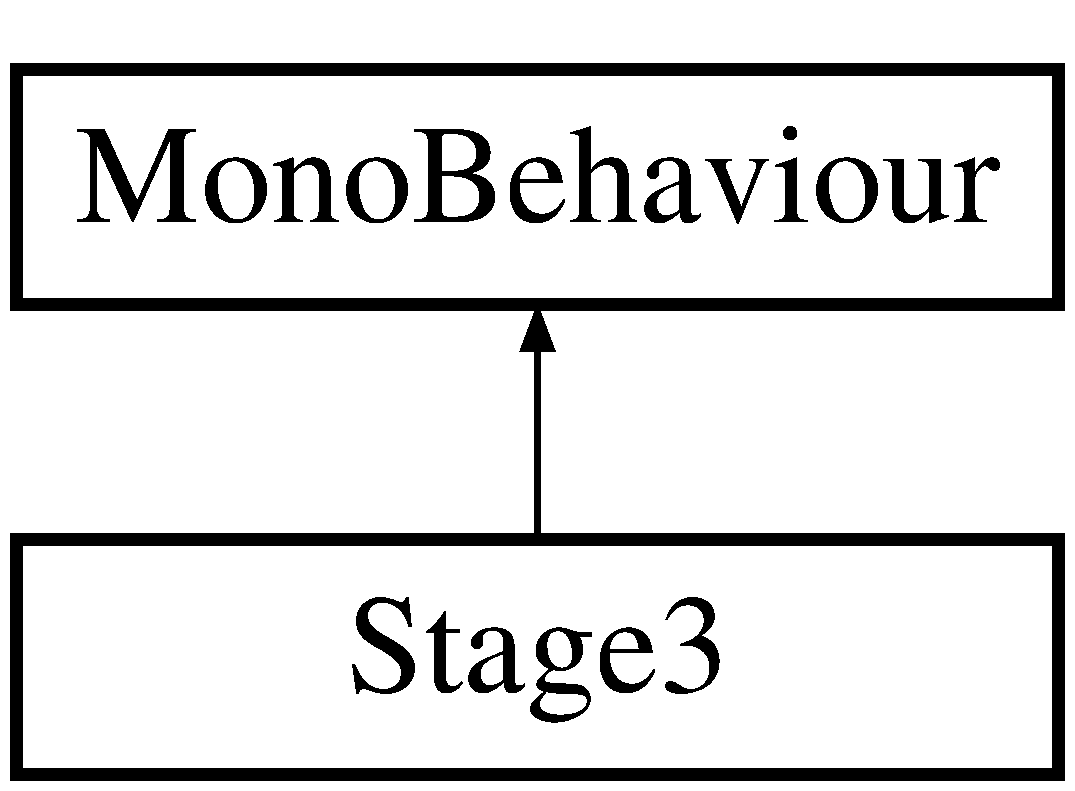
\includegraphics[height=2.000000cm]{class_stage3}
\end{center}
\end{figure}
\subsection*{Static Public Attributes}
\begin{DoxyCompactItemize}
\item 
static \mbox{\hyperlink{class_stage3}{Stage3}} \mbox{\hyperlink{class_stage3_ad7d6de393aa63c520bcbf0385ace2217}{s\+\_\+\+Instance}} = null
\end{DoxyCompactItemize}
\subsection*{Private Member Functions}
\begin{DoxyCompactItemize}
\item 
void \mbox{\hyperlink{class_stage3_a2055cf61814f4e7a414bc971c7ab81eb}{Start}} ()
\item 
void \mbox{\hyperlink{class_stage3_a52931a93bc0d482e2addeda6f41b7d6c}{On\+Enable}} ()
\item 
void \mbox{\hyperlink{class_stage3_a41463491a3a1b6640d0cc22a19de2dfa}{On\+Disable}} ()
\item 
void \mbox{\hyperlink{class_stage3_a5c1a079dcce9bb1d77bfe427d82d705c}{Button\+Was\+Clicked}} ()
\begin{DoxyCompactList}\small\item\em This gets called when the user clicks the button \end{DoxyCompactList}\item 
void \mbox{\hyperlink{class_stage3_a71d7781de4de72fb87bc733c1143d4c4}{Update}} ()
\item 
I\+Enumerator \mbox{\hyperlink{class_stage3_a3ebce4adf62b36d8987f00fe73a37a38}{Run}} ()
\begin{DoxyCompactList}\small\item\em Controls the flow of the scene. \end{DoxyCompactList}\end{DoxyCompactItemize}
\subsection*{Private Attributes}
\begin{DoxyCompactItemize}
\item 
\mbox{\hyperlink{class_intro_session_manager}{Intro\+Session\+Manager}} \mbox{\hyperlink{class_stage3_a60a220a150389131070a070cc3347e05}{m\+\_\+\+Manager}}
\item 
\mbox{\hyperlink{class_v_r_standard_assets_1_1_utils_1_1_raycaster_v_r}{Raycaster\+VR}} \mbox{\hyperlink{class_stage3_a5c4d1688c502ea8bd4c753b2218c4007}{m\+\_\+\+Raycaster\+Script}}
\item 
readonly Vector3 \mbox{\hyperlink{class_stage3_a6a0ce3270dd4215a5cd38b3d5e81e723}{c\+\_\+\+Robot\+Location\+Near\+Button}} = new Vector3(2.\+68f, 3.\+13f, 6.\+22f)
\item 
\mbox{\hyperlink{class_dialogue}{Dialogue}} \mbox{\hyperlink{class_stage3_aab381d5b8a47d993bb82777b6792866f}{m\+\_\+\+Dialogue\+Instructions}}
\item 
\mbox{\hyperlink{class_dialogue}{Dialogue}} \mbox{\hyperlink{class_stage3_af1a5f4e00ee60f23f0d28fd02d671127}{m\+\_\+\+Dialogue\+Fail}}
\item 
int \mbox{\hyperlink{class_stage3_aeb53b781e0caf8b3eb317a5044514932}{m\+\_\+\+Button\+Clicks}}
\item 
bool \mbox{\hyperlink{class_stage3_a62ef9acb64218865668a01d54d8a3705}{m\+\_\+\+Can\+Hit\+Button}} = true
\end{DoxyCompactItemize}


\subsection{Member Function Documentation}
\mbox{\Hypertarget{class_stage3_a5c1a079dcce9bb1d77bfe427d82d705c}\label{class_stage3_a5c1a079dcce9bb1d77bfe427d82d705c}} 
\index{Stage3@{Stage3}!Button\+Was\+Clicked@{Button\+Was\+Clicked}}
\index{Button\+Was\+Clicked@{Button\+Was\+Clicked}!Stage3@{Stage3}}
\subsubsection{\texorpdfstring{Button\+Was\+Clicked()}{ButtonWasClicked()}}
{\footnotesize\ttfamily void Stage3.\+Button\+Was\+Clicked (\begin{DoxyParamCaption}{ }\end{DoxyParamCaption})\hspace{0.3cm}{\ttfamily [private]}}



This gets called when the user clicks the button 

\mbox{\Hypertarget{class_stage3_a41463491a3a1b6640d0cc22a19de2dfa}\label{class_stage3_a41463491a3a1b6640d0cc22a19de2dfa}} 
\index{Stage3@{Stage3}!On\+Disable@{On\+Disable}}
\index{On\+Disable@{On\+Disable}!Stage3@{Stage3}}
\subsubsection{\texorpdfstring{On\+Disable()}{OnDisable()}}
{\footnotesize\ttfamily void Stage3.\+On\+Disable (\begin{DoxyParamCaption}{ }\end{DoxyParamCaption})\hspace{0.3cm}{\ttfamily [private]}}

\mbox{\Hypertarget{class_stage3_a52931a93bc0d482e2addeda6f41b7d6c}\label{class_stage3_a52931a93bc0d482e2addeda6f41b7d6c}} 
\index{Stage3@{Stage3}!On\+Enable@{On\+Enable}}
\index{On\+Enable@{On\+Enable}!Stage3@{Stage3}}
\subsubsection{\texorpdfstring{On\+Enable()}{OnEnable()}}
{\footnotesize\ttfamily void Stage3.\+On\+Enable (\begin{DoxyParamCaption}{ }\end{DoxyParamCaption})\hspace{0.3cm}{\ttfamily [private]}}

\mbox{\Hypertarget{class_stage3_a3ebce4adf62b36d8987f00fe73a37a38}\label{class_stage3_a3ebce4adf62b36d8987f00fe73a37a38}} 
\index{Stage3@{Stage3}!Run@{Run}}
\index{Run@{Run}!Stage3@{Stage3}}
\subsubsection{\texorpdfstring{Run()}{Run()}}
{\footnotesize\ttfamily I\+Enumerator Stage3.\+Run (\begin{DoxyParamCaption}{ }\end{DoxyParamCaption})\hspace{0.3cm}{\ttfamily [private]}}



Controls the flow of the scene. 

\begin{DoxyReturn}{Returns}
A reference to the coroutine
\end{DoxyReturn}
\mbox{\Hypertarget{class_stage3_a2055cf61814f4e7a414bc971c7ab81eb}\label{class_stage3_a2055cf61814f4e7a414bc971c7ab81eb}} 
\index{Stage3@{Stage3}!Start@{Start}}
\index{Start@{Start}!Stage3@{Stage3}}
\subsubsection{\texorpdfstring{Start()}{Start()}}
{\footnotesize\ttfamily void Stage3.\+Start (\begin{DoxyParamCaption}{ }\end{DoxyParamCaption})\hspace{0.3cm}{\ttfamily [private]}}

\mbox{\Hypertarget{class_stage3_a71d7781de4de72fb87bc733c1143d4c4}\label{class_stage3_a71d7781de4de72fb87bc733c1143d4c4}} 
\index{Stage3@{Stage3}!Update@{Update}}
\index{Update@{Update}!Stage3@{Stage3}}
\subsubsection{\texorpdfstring{Update()}{Update()}}
{\footnotesize\ttfamily void Stage3.\+Update (\begin{DoxyParamCaption}{ }\end{DoxyParamCaption})\hspace{0.3cm}{\ttfamily [private]}}



\subsection{Member Data Documentation}
\mbox{\Hypertarget{class_stage3_a6a0ce3270dd4215a5cd38b3d5e81e723}\label{class_stage3_a6a0ce3270dd4215a5cd38b3d5e81e723}} 
\index{Stage3@{Stage3}!c\+\_\+\+Robot\+Location\+Near\+Button@{c\+\_\+\+Robot\+Location\+Near\+Button}}
\index{c\+\_\+\+Robot\+Location\+Near\+Button@{c\+\_\+\+Robot\+Location\+Near\+Button}!Stage3@{Stage3}}
\subsubsection{\texorpdfstring{c\+\_\+\+Robot\+Location\+Near\+Button}{c\_RobotLocationNearButton}}
{\footnotesize\ttfamily readonly Vector3 Stage3.\+c\+\_\+\+Robot\+Location\+Near\+Button = new Vector3(2.\+68f, 3.\+13f, 6.\+22f)\hspace{0.3cm}{\ttfamily [private]}}

\mbox{\Hypertarget{class_stage3_aeb53b781e0caf8b3eb317a5044514932}\label{class_stage3_aeb53b781e0caf8b3eb317a5044514932}} 
\index{Stage3@{Stage3}!m\+\_\+\+Button\+Clicks@{m\+\_\+\+Button\+Clicks}}
\index{m\+\_\+\+Button\+Clicks@{m\+\_\+\+Button\+Clicks}!Stage3@{Stage3}}
\subsubsection{\texorpdfstring{m\+\_\+\+Button\+Clicks}{m\_ButtonClicks}}
{\footnotesize\ttfamily int Stage3.\+m\+\_\+\+Button\+Clicks\hspace{0.3cm}{\ttfamily [private]}}

\mbox{\Hypertarget{class_stage3_a62ef9acb64218865668a01d54d8a3705}\label{class_stage3_a62ef9acb64218865668a01d54d8a3705}} 
\index{Stage3@{Stage3}!m\+\_\+\+Can\+Hit\+Button@{m\+\_\+\+Can\+Hit\+Button}}
\index{m\+\_\+\+Can\+Hit\+Button@{m\+\_\+\+Can\+Hit\+Button}!Stage3@{Stage3}}
\subsubsection{\texorpdfstring{m\+\_\+\+Can\+Hit\+Button}{m\_CanHitButton}}
{\footnotesize\ttfamily bool Stage3.\+m\+\_\+\+Can\+Hit\+Button = true\hspace{0.3cm}{\ttfamily [private]}}

\mbox{\Hypertarget{class_stage3_af1a5f4e00ee60f23f0d28fd02d671127}\label{class_stage3_af1a5f4e00ee60f23f0d28fd02d671127}} 
\index{Stage3@{Stage3}!m\+\_\+\+Dialogue\+Fail@{m\+\_\+\+Dialogue\+Fail}}
\index{m\+\_\+\+Dialogue\+Fail@{m\+\_\+\+Dialogue\+Fail}!Stage3@{Stage3}}
\subsubsection{\texorpdfstring{m\+\_\+\+Dialogue\+Fail}{m\_DialogueFail}}
{\footnotesize\ttfamily \mbox{\hyperlink{class_dialogue}{Dialogue}} Stage3.\+m\+\_\+\+Dialogue\+Fail\hspace{0.3cm}{\ttfamily [private]}}

\mbox{\Hypertarget{class_stage3_aab381d5b8a47d993bb82777b6792866f}\label{class_stage3_aab381d5b8a47d993bb82777b6792866f}} 
\index{Stage3@{Stage3}!m\+\_\+\+Dialogue\+Instructions@{m\+\_\+\+Dialogue\+Instructions}}
\index{m\+\_\+\+Dialogue\+Instructions@{m\+\_\+\+Dialogue\+Instructions}!Stage3@{Stage3}}
\subsubsection{\texorpdfstring{m\+\_\+\+Dialogue\+Instructions}{m\_DialogueInstructions}}
{\footnotesize\ttfamily \mbox{\hyperlink{class_dialogue}{Dialogue}} Stage3.\+m\+\_\+\+Dialogue\+Instructions\hspace{0.3cm}{\ttfamily [private]}}

\mbox{\Hypertarget{class_stage3_a60a220a150389131070a070cc3347e05}\label{class_stage3_a60a220a150389131070a070cc3347e05}} 
\index{Stage3@{Stage3}!m\+\_\+\+Manager@{m\+\_\+\+Manager}}
\index{m\+\_\+\+Manager@{m\+\_\+\+Manager}!Stage3@{Stage3}}
\subsubsection{\texorpdfstring{m\+\_\+\+Manager}{m\_Manager}}
{\footnotesize\ttfamily \mbox{\hyperlink{class_intro_session_manager}{Intro\+Session\+Manager}} Stage3.\+m\+\_\+\+Manager\hspace{0.3cm}{\ttfamily [private]}}

\mbox{\Hypertarget{class_stage3_a5c4d1688c502ea8bd4c753b2218c4007}\label{class_stage3_a5c4d1688c502ea8bd4c753b2218c4007}} 
\index{Stage3@{Stage3}!m\+\_\+\+Raycaster\+Script@{m\+\_\+\+Raycaster\+Script}}
\index{m\+\_\+\+Raycaster\+Script@{m\+\_\+\+Raycaster\+Script}!Stage3@{Stage3}}
\subsubsection{\texorpdfstring{m\+\_\+\+Raycaster\+Script}{m\_RaycasterScript}}
{\footnotesize\ttfamily \mbox{\hyperlink{class_v_r_standard_assets_1_1_utils_1_1_raycaster_v_r}{Raycaster\+VR}} Stage3.\+m\+\_\+\+Raycaster\+Script\hspace{0.3cm}{\ttfamily [private]}}

\mbox{\Hypertarget{class_stage3_ad7d6de393aa63c520bcbf0385ace2217}\label{class_stage3_ad7d6de393aa63c520bcbf0385ace2217}} 
\index{Stage3@{Stage3}!s\+\_\+\+Instance@{s\+\_\+\+Instance}}
\index{s\+\_\+\+Instance@{s\+\_\+\+Instance}!Stage3@{Stage3}}
\subsubsection{\texorpdfstring{s\+\_\+\+Instance}{s\_Instance}}
{\footnotesize\ttfamily \mbox{\hyperlink{class_stage3}{Stage3}} Stage3.\+s\+\_\+\+Instance = null\hspace{0.3cm}{\ttfamily [static]}}



The documentation for this class was generated from the following file\+:\begin{DoxyCompactItemize}
\item 
\mbox{\hyperlink{_stage3_8cs}{Stage3.\+cs}}\end{DoxyCompactItemize}

\hypertarget{class_stage4}{}\section{Stage4 Class Reference}
\label{class_stage4}\index{Stage4@{Stage4}}
Inheritance diagram for Stage4\+:\begin{figure}[H]
\begin{center}
\leavevmode
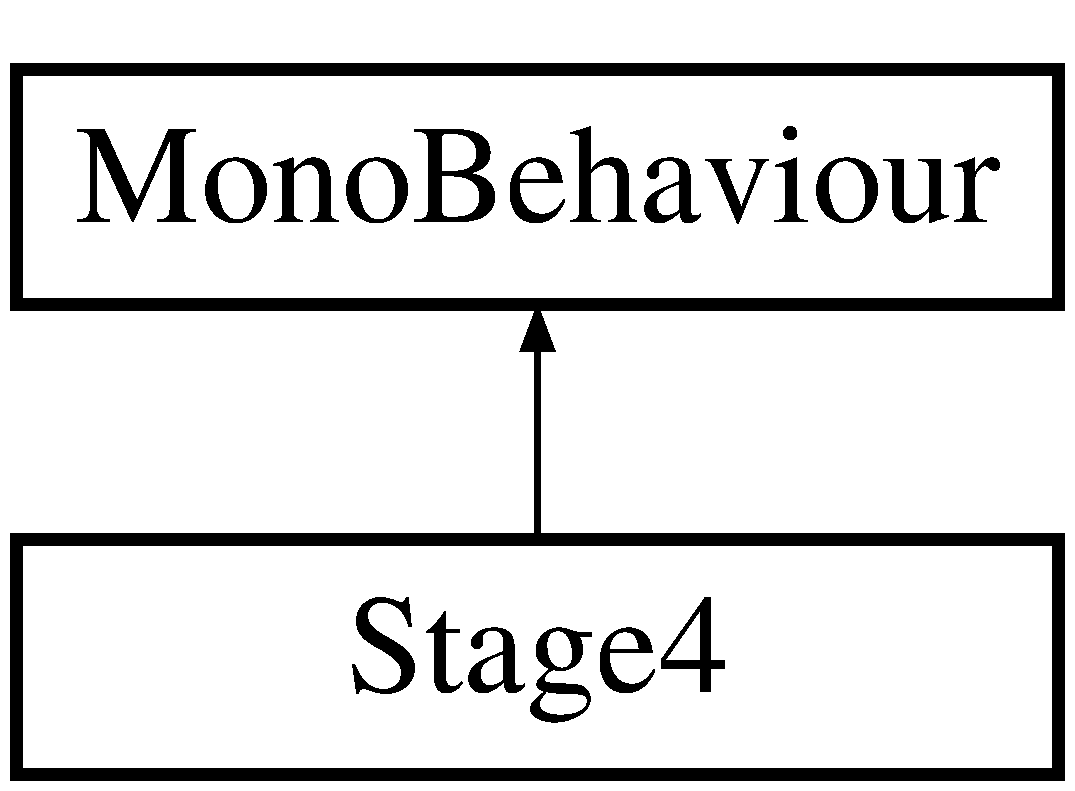
\includegraphics[height=2.000000cm]{class_stage4}
\end{center}
\end{figure}
\subsection*{Public Member Functions}
\begin{DoxyCompactItemize}
\item 
void \mbox{\hyperlink{class_stage4_a3b96ad980e2129d1fcb619673921c233}{Notify\+Ball\+Trigger}} ()
\begin{DoxyCompactList}\small\item\em Gets called when the user drops the ball through the trap doors \end{DoxyCompactList}\end{DoxyCompactItemize}
\subsection*{Static Public Attributes}
\begin{DoxyCompactItemize}
\item 
static \mbox{\hyperlink{class_stage4}{Stage4}} \mbox{\hyperlink{class_stage4_a34780e013df9edac711f8b62d9c9a629}{s\+\_\+\+Instance}} = null
\end{DoxyCompactItemize}
\subsection*{Private Member Functions}
\begin{DoxyCompactItemize}
\item 
void \mbox{\hyperlink{class_stage4_a24aafa249875c3bd1a1383d2eb40c79e}{Start}} ()
\item 
void \mbox{\hyperlink{class_stage4_ace16b39395d5c08775c8e031c0e76aa2}{On\+Enable}} ()
\item 
void \mbox{\hyperlink{class_stage4_a2746354b2a72b27e3add3f0f4c7f5160}{On\+Disable}} ()
\item 
void \mbox{\hyperlink{class_stage4_a32fad5731207055e6b5630a59076dcfd}{Ball\+Dropped}} ()
\begin{DoxyCompactList}\small\item\em Called when the ball has been dropped. \end{DoxyCompactList}\item 
void \mbox{\hyperlink{class_stage4_aeb84711e7a42d39c057d74c7d7a1fe17}{Ball\+Picked\+Up}} ()
\begin{DoxyCompactList}\small\item\em Called when the ball is picked up \end{DoxyCompactList}\item 
void \mbox{\hyperlink{class_stage4_a6772bbc4255878e6c0987c8876e547b7}{Update}} ()
\item 
void \mbox{\hyperlink{class_stage4_a972d03f467d6ce6fd2de56b541b85a3b}{End\+Of\+Stage}} ()
\begin{DoxyCompactList}\small\item\em Ends the stage, closes the trap doors, and advances to the next scene \end{DoxyCompactList}\end{DoxyCompactItemize}
\subsection*{Private Attributes}
\begin{DoxyCompactItemize}
\item 
\mbox{\hyperlink{class_v_r_standard_assets_1_1_utils_1_1_raycaster_v_r}{Raycaster\+VR}} \mbox{\hyperlink{class_stage4_a7ac8343ac248e658b20a135aa7771cf1}{m\+\_\+\+Raycaster\+Script}}
\item 
\mbox{\hyperlink{class_intro_session_manager}{Intro\+Session\+Manager}} \mbox{\hyperlink{class_stage4_a8f131659124d1b84a702b7a2b2b5b5ad}{m\+\_\+\+Manager}}
\item 
\mbox{\hyperlink{class_dialogue}{Dialogue}} \mbox{\hyperlink{class_stage4_a8862f5c33367530940185e68a778bb4a}{m\+\_\+\+Dialogue\+Instructions}}
\item 
\mbox{\hyperlink{class_dialogue}{Dialogue}} \mbox{\hyperlink{class_stage4_aae05efed193bd950fd9bf3c8b6d9e438}{m\+\_\+\+Dialogue\+Fail}}
\item 
int \mbox{\hyperlink{class_stage4_abca0599ad45f84b0cfa068aee6e10fa2}{m\+\_\+ball\+Dropped\+Count}} = 0
\item 
bool \mbox{\hyperlink{class_stage4_ae0bebd4e94c3f743c7e81af16042fe6d}{m\+\_\+is\+End}}
\item 
float \mbox{\hyperlink{class_stage4_a49602aa6588e4e288a1fda3ea03987a7}{m\+\_\+timer}}
\end{DoxyCompactItemize}


\subsection{Member Function Documentation}
\mbox{\Hypertarget{class_stage4_a32fad5731207055e6b5630a59076dcfd}\label{class_stage4_a32fad5731207055e6b5630a59076dcfd}} 
\index{Stage4@{Stage4}!Ball\+Dropped@{Ball\+Dropped}}
\index{Ball\+Dropped@{Ball\+Dropped}!Stage4@{Stage4}}
\subsubsection{\texorpdfstring{Ball\+Dropped()}{BallDropped()}}
{\footnotesize\ttfamily void Stage4.\+Ball\+Dropped (\begin{DoxyParamCaption}{ }\end{DoxyParamCaption})\hspace{0.3cm}{\ttfamily [private]}}



Called when the ball has been dropped. 

\mbox{\Hypertarget{class_stage4_aeb84711e7a42d39c057d74c7d7a1fe17}\label{class_stage4_aeb84711e7a42d39c057d74c7d7a1fe17}} 
\index{Stage4@{Stage4}!Ball\+Picked\+Up@{Ball\+Picked\+Up}}
\index{Ball\+Picked\+Up@{Ball\+Picked\+Up}!Stage4@{Stage4}}
\subsubsection{\texorpdfstring{Ball\+Picked\+Up()}{BallPickedUp()}}
{\footnotesize\ttfamily void Stage4.\+Ball\+Picked\+Up (\begin{DoxyParamCaption}{ }\end{DoxyParamCaption})\hspace{0.3cm}{\ttfamily [private]}}



Called when the ball is picked up 

\mbox{\Hypertarget{class_stage4_a972d03f467d6ce6fd2de56b541b85a3b}\label{class_stage4_a972d03f467d6ce6fd2de56b541b85a3b}} 
\index{Stage4@{Stage4}!End\+Of\+Stage@{End\+Of\+Stage}}
\index{End\+Of\+Stage@{End\+Of\+Stage}!Stage4@{Stage4}}
\subsubsection{\texorpdfstring{End\+Of\+Stage()}{EndOfStage()}}
{\footnotesize\ttfamily void Stage4.\+End\+Of\+Stage (\begin{DoxyParamCaption}{ }\end{DoxyParamCaption})\hspace{0.3cm}{\ttfamily [private]}}



Ends the stage, closes the trap doors, and advances to the next scene 

\mbox{\Hypertarget{class_stage4_a3b96ad980e2129d1fcb619673921c233}\label{class_stage4_a3b96ad980e2129d1fcb619673921c233}} 
\index{Stage4@{Stage4}!Notify\+Ball\+Trigger@{Notify\+Ball\+Trigger}}
\index{Notify\+Ball\+Trigger@{Notify\+Ball\+Trigger}!Stage4@{Stage4}}
\subsubsection{\texorpdfstring{Notify\+Ball\+Trigger()}{NotifyBallTrigger()}}
{\footnotesize\ttfamily void Stage4.\+Notify\+Ball\+Trigger (\begin{DoxyParamCaption}{ }\end{DoxyParamCaption})}



Gets called when the user drops the ball through the trap doors 

\mbox{\Hypertarget{class_stage4_a2746354b2a72b27e3add3f0f4c7f5160}\label{class_stage4_a2746354b2a72b27e3add3f0f4c7f5160}} 
\index{Stage4@{Stage4}!On\+Disable@{On\+Disable}}
\index{On\+Disable@{On\+Disable}!Stage4@{Stage4}}
\subsubsection{\texorpdfstring{On\+Disable()}{OnDisable()}}
{\footnotesize\ttfamily void Stage4.\+On\+Disable (\begin{DoxyParamCaption}{ }\end{DoxyParamCaption})\hspace{0.3cm}{\ttfamily [private]}}

\mbox{\Hypertarget{class_stage4_ace16b39395d5c08775c8e031c0e76aa2}\label{class_stage4_ace16b39395d5c08775c8e031c0e76aa2}} 
\index{Stage4@{Stage4}!On\+Enable@{On\+Enable}}
\index{On\+Enable@{On\+Enable}!Stage4@{Stage4}}
\subsubsection{\texorpdfstring{On\+Enable()}{OnEnable()}}
{\footnotesize\ttfamily void Stage4.\+On\+Enable (\begin{DoxyParamCaption}{ }\end{DoxyParamCaption})\hspace{0.3cm}{\ttfamily [private]}}

\mbox{\Hypertarget{class_stage4_a24aafa249875c3bd1a1383d2eb40c79e}\label{class_stage4_a24aafa249875c3bd1a1383d2eb40c79e}} 
\index{Stage4@{Stage4}!Start@{Start}}
\index{Start@{Start}!Stage4@{Stage4}}
\subsubsection{\texorpdfstring{Start()}{Start()}}
{\footnotesize\ttfamily void Stage4.\+Start (\begin{DoxyParamCaption}{ }\end{DoxyParamCaption})\hspace{0.3cm}{\ttfamily [private]}}

\mbox{\Hypertarget{class_stage4_a6772bbc4255878e6c0987c8876e547b7}\label{class_stage4_a6772bbc4255878e6c0987c8876e547b7}} 
\index{Stage4@{Stage4}!Update@{Update}}
\index{Update@{Update}!Stage4@{Stage4}}
\subsubsection{\texorpdfstring{Update()}{Update()}}
{\footnotesize\ttfamily void Stage4.\+Update (\begin{DoxyParamCaption}{ }\end{DoxyParamCaption})\hspace{0.3cm}{\ttfamily [private]}}



\subsection{Member Data Documentation}
\mbox{\Hypertarget{class_stage4_abca0599ad45f84b0cfa068aee6e10fa2}\label{class_stage4_abca0599ad45f84b0cfa068aee6e10fa2}} 
\index{Stage4@{Stage4}!m\+\_\+ball\+Dropped\+Count@{m\+\_\+ball\+Dropped\+Count}}
\index{m\+\_\+ball\+Dropped\+Count@{m\+\_\+ball\+Dropped\+Count}!Stage4@{Stage4}}
\subsubsection{\texorpdfstring{m\+\_\+ball\+Dropped\+Count}{m\_ballDroppedCount}}
{\footnotesize\ttfamily int Stage4.\+m\+\_\+ball\+Dropped\+Count = 0\hspace{0.3cm}{\ttfamily [private]}}

\mbox{\Hypertarget{class_stage4_aae05efed193bd950fd9bf3c8b6d9e438}\label{class_stage4_aae05efed193bd950fd9bf3c8b6d9e438}} 
\index{Stage4@{Stage4}!m\+\_\+\+Dialogue\+Fail@{m\+\_\+\+Dialogue\+Fail}}
\index{m\+\_\+\+Dialogue\+Fail@{m\+\_\+\+Dialogue\+Fail}!Stage4@{Stage4}}
\subsubsection{\texorpdfstring{m\+\_\+\+Dialogue\+Fail}{m\_DialogueFail}}
{\footnotesize\ttfamily \mbox{\hyperlink{class_dialogue}{Dialogue}} Stage4.\+m\+\_\+\+Dialogue\+Fail\hspace{0.3cm}{\ttfamily [private]}}

\mbox{\Hypertarget{class_stage4_a8862f5c33367530940185e68a778bb4a}\label{class_stage4_a8862f5c33367530940185e68a778bb4a}} 
\index{Stage4@{Stage4}!m\+\_\+\+Dialogue\+Instructions@{m\+\_\+\+Dialogue\+Instructions}}
\index{m\+\_\+\+Dialogue\+Instructions@{m\+\_\+\+Dialogue\+Instructions}!Stage4@{Stage4}}
\subsubsection{\texorpdfstring{m\+\_\+\+Dialogue\+Instructions}{m\_DialogueInstructions}}
{\footnotesize\ttfamily \mbox{\hyperlink{class_dialogue}{Dialogue}} Stage4.\+m\+\_\+\+Dialogue\+Instructions\hspace{0.3cm}{\ttfamily [private]}}

\mbox{\Hypertarget{class_stage4_ae0bebd4e94c3f743c7e81af16042fe6d}\label{class_stage4_ae0bebd4e94c3f743c7e81af16042fe6d}} 
\index{Stage4@{Stage4}!m\+\_\+is\+End@{m\+\_\+is\+End}}
\index{m\+\_\+is\+End@{m\+\_\+is\+End}!Stage4@{Stage4}}
\subsubsection{\texorpdfstring{m\+\_\+is\+End}{m\_isEnd}}
{\footnotesize\ttfamily bool Stage4.\+m\+\_\+is\+End\hspace{0.3cm}{\ttfamily [private]}}

\mbox{\Hypertarget{class_stage4_a8f131659124d1b84a702b7a2b2b5b5ad}\label{class_stage4_a8f131659124d1b84a702b7a2b2b5b5ad}} 
\index{Stage4@{Stage4}!m\+\_\+\+Manager@{m\+\_\+\+Manager}}
\index{m\+\_\+\+Manager@{m\+\_\+\+Manager}!Stage4@{Stage4}}
\subsubsection{\texorpdfstring{m\+\_\+\+Manager}{m\_Manager}}
{\footnotesize\ttfamily \mbox{\hyperlink{class_intro_session_manager}{Intro\+Session\+Manager}} Stage4.\+m\+\_\+\+Manager\hspace{0.3cm}{\ttfamily [private]}}

\mbox{\Hypertarget{class_stage4_a7ac8343ac248e658b20a135aa7771cf1}\label{class_stage4_a7ac8343ac248e658b20a135aa7771cf1}} 
\index{Stage4@{Stage4}!m\+\_\+\+Raycaster\+Script@{m\+\_\+\+Raycaster\+Script}}
\index{m\+\_\+\+Raycaster\+Script@{m\+\_\+\+Raycaster\+Script}!Stage4@{Stage4}}
\subsubsection{\texorpdfstring{m\+\_\+\+Raycaster\+Script}{m\_RaycasterScript}}
{\footnotesize\ttfamily \mbox{\hyperlink{class_v_r_standard_assets_1_1_utils_1_1_raycaster_v_r}{Raycaster\+VR}} Stage4.\+m\+\_\+\+Raycaster\+Script\hspace{0.3cm}{\ttfamily [private]}}

\mbox{\Hypertarget{class_stage4_a49602aa6588e4e288a1fda3ea03987a7}\label{class_stage4_a49602aa6588e4e288a1fda3ea03987a7}} 
\index{Stage4@{Stage4}!m\+\_\+timer@{m\+\_\+timer}}
\index{m\+\_\+timer@{m\+\_\+timer}!Stage4@{Stage4}}
\subsubsection{\texorpdfstring{m\+\_\+timer}{m\_timer}}
{\footnotesize\ttfamily float Stage4.\+m\+\_\+timer\hspace{0.3cm}{\ttfamily [private]}}

\mbox{\Hypertarget{class_stage4_a34780e013df9edac711f8b62d9c9a629}\label{class_stage4_a34780e013df9edac711f8b62d9c9a629}} 
\index{Stage4@{Stage4}!s\+\_\+\+Instance@{s\+\_\+\+Instance}}
\index{s\+\_\+\+Instance@{s\+\_\+\+Instance}!Stage4@{Stage4}}
\subsubsection{\texorpdfstring{s\+\_\+\+Instance}{s\_Instance}}
{\footnotesize\ttfamily \mbox{\hyperlink{class_stage4}{Stage4}} Stage4.\+s\+\_\+\+Instance = null\hspace{0.3cm}{\ttfamily [static]}}



The documentation for this class was generated from the following file\+:\begin{DoxyCompactItemize}
\item 
\mbox{\hyperlink{_stage4_8cs}{Stage4.\+cs}}\end{DoxyCompactItemize}

\hypertarget{class_stage5}{}\section{Stage5 Class Reference}
\label{class_stage5}\index{Stage5@{Stage5}}
Inheritance diagram for Stage5\+:\begin{figure}[H]
\begin{center}
\leavevmode
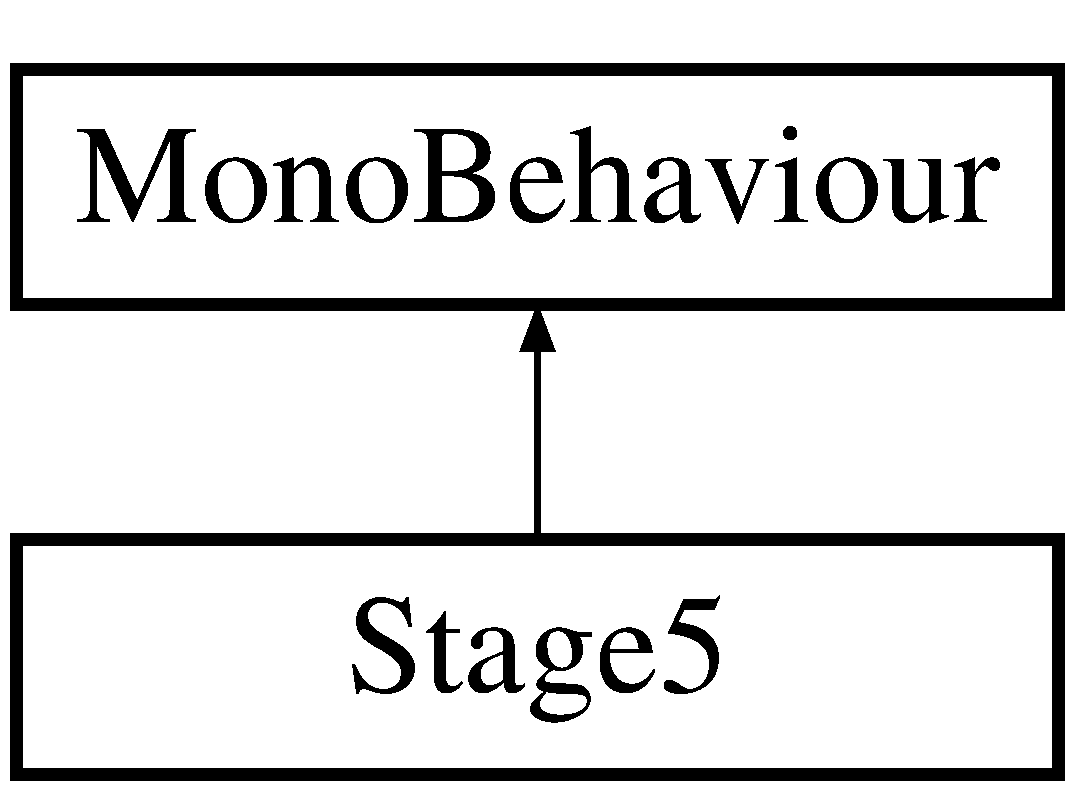
\includegraphics[height=2.000000cm]{class_stage5}
\end{center}
\end{figure}
\subsection*{Static Public Attributes}
\begin{DoxyCompactItemize}
\item 
static \mbox{\hyperlink{class_stage5}{Stage5}} \mbox{\hyperlink{class_stage5_a11ae41443d21c56ceb47e96d8c2f06a4}{s\+\_\+\+Instance}} = null
\end{DoxyCompactItemize}
\subsection*{Private Member Functions}
\begin{DoxyCompactItemize}
\item 
void \mbox{\hyperlink{class_stage5_ac70bd321f425cb2917a1e8a20cba8524}{Start}} ()
\item 
void \mbox{\hyperlink{class_stage5_ac5bc96024542fdf588a18a7e6de7892f}{On\+Enable}} ()
\begin{DoxyCompactList}\small\item\em Called when the script is enabled, subscribes to events triggered in V\+R\+Eye\+Raycaster \end{DoxyCompactList}\item 
void \mbox{\hyperlink{class_stage5_afd72a075c088e399a206482e8be39cce}{On\+Disable}} ()
\begin{DoxyCompactList}\small\item\em Called when the script is enabled, unsubscribes to events triggered in V\+R\+Eye\+Raycaster \end{DoxyCompactList}\item 
void \mbox{\hyperlink{class_stage5_a1cdfae544606e8537d2dd31e5ed2ea83}{Complete\+Stage}} ()
\begin{DoxyCompactList}\small\item\em Called when the ball is thrown and the event is triggered. Will end the stage. \end{DoxyCompactList}\item 
void \mbox{\hyperlink{class_stage5_a0d60946476d491834a1f2e41e74da306}{Ball\+Dropped}} ()
\begin{DoxyCompactList}\small\item\em Triggered by an event when the ball has been dropped \end{DoxyCompactList}\item 
void \mbox{\hyperlink{class_stage5_a06516c2e958f8fea48f5d88924649ba4}{Ball\+Picked\+Up}} ()
\begin{DoxyCompactList}\small\item\em Triggered by an event when the ball has been picked up \end{DoxyCompactList}\item 
void \mbox{\hyperlink{class_stage5_a1eff3e21d86d4460f57f86e692f50af3}{Update}} ()
\item 
void \mbox{\hyperlink{class_stage5_a36b22a4efd98ae6ba0b0b4cd9e058094}{Run}} ()
\begin{DoxyCompactList}\small\item\em Controls the flow of the scene. \end{DoxyCompactList}\item 
I\+Enumerator \mbox{\hyperlink{class_stage5_ab2e381c47a40f2726df0579f07bbb7fa}{Check\+For\+Fails}} ()
\begin{DoxyCompactList}\small\item\em Waits and checks if the user hasn\textquotesingle{}t picked up the ball yet and informs them to do so after 15 seconds \end{DoxyCompactList}\item 
void \mbox{\hyperlink{class_stage5_a648d6f5b7fe35e437694c010f8b4704f}{End\+Scene}} ()
\begin{DoxyCompactList}\small\item\em Ends the scene and moves on to the next one \end{DoxyCompactList}\end{DoxyCompactItemize}
\subsection*{Private Attributes}
\begin{DoxyCompactItemize}
\item 
\mbox{\hyperlink{class_intro_session_manager}{Intro\+Session\+Manager}} \mbox{\hyperlink{class_stage5_a7f6c6334d936500cd2c2c0510c3b9c8f}{m\+\_\+\+Manager}}
\item 
\mbox{\hyperlink{class_v_r_standard_assets_1_1_utils_1_1_raycaster_v_r}{Raycaster\+VR}} \mbox{\hyperlink{class_stage5_a1bb51309966ab470df9b3229046332e1}{m\+\_\+\+Raycaster\+Script}}
\item 
\mbox{\hyperlink{class_dialogue}{Dialogue}} \mbox{\hyperlink{class_stage5_a74caa3de0c1bef9476af55d329b542a3}{m\+\_\+\+Dialogue\+Instructions}}
\item 
\mbox{\hyperlink{class_dialogue}{Dialogue}} \mbox{\hyperlink{class_stage5_abb8bc51393ba9348ad464d7bd0f97e5d}{m\+\_\+\+Dialogue\+Fail}}
\item 
bool \mbox{\hyperlink{class_stage5_a51c1395cdadb3828f7682f59560ee6b1}{m\+\_\+\+Is\+Ball\+Thrown}}
\item 
bool \mbox{\hyperlink{class_stage5_a84c27763b680c4c9086c5facf3302e1d}{m\+\_\+\+Is\+End}}
\item 
int \mbox{\hyperlink{class_stage5_a845a29cee8d9154d559ca52b8f0fd788}{m\+\_\+\+Ball\+Dropped\+Count}} = 0
\end{DoxyCompactItemize}


\subsection{Member Function Documentation}
\mbox{\Hypertarget{class_stage5_a0d60946476d491834a1f2e41e74da306}\label{class_stage5_a0d60946476d491834a1f2e41e74da306}} 
\index{Stage5@{Stage5}!Ball\+Dropped@{Ball\+Dropped}}
\index{Ball\+Dropped@{Ball\+Dropped}!Stage5@{Stage5}}
\subsubsection{\texorpdfstring{Ball\+Dropped()}{BallDropped()}}
{\footnotesize\ttfamily void Stage5.\+Ball\+Dropped (\begin{DoxyParamCaption}{ }\end{DoxyParamCaption})\hspace{0.3cm}{\ttfamily [private]}}



Triggered by an event when the ball has been dropped 

\mbox{\Hypertarget{class_stage5_a06516c2e958f8fea48f5d88924649ba4}\label{class_stage5_a06516c2e958f8fea48f5d88924649ba4}} 
\index{Stage5@{Stage5}!Ball\+Picked\+Up@{Ball\+Picked\+Up}}
\index{Ball\+Picked\+Up@{Ball\+Picked\+Up}!Stage5@{Stage5}}
\subsubsection{\texorpdfstring{Ball\+Picked\+Up()}{BallPickedUp()}}
{\footnotesize\ttfamily void Stage5.\+Ball\+Picked\+Up (\begin{DoxyParamCaption}{ }\end{DoxyParamCaption})\hspace{0.3cm}{\ttfamily [private]}}



Triggered by an event when the ball has been picked up 

\mbox{\Hypertarget{class_stage5_ab2e381c47a40f2726df0579f07bbb7fa}\label{class_stage5_ab2e381c47a40f2726df0579f07bbb7fa}} 
\index{Stage5@{Stage5}!Check\+For\+Fails@{Check\+For\+Fails}}
\index{Check\+For\+Fails@{Check\+For\+Fails}!Stage5@{Stage5}}
\subsubsection{\texorpdfstring{Check\+For\+Fails()}{CheckForFails()}}
{\footnotesize\ttfamily I\+Enumerator Stage5.\+Check\+For\+Fails (\begin{DoxyParamCaption}{ }\end{DoxyParamCaption})\hspace{0.3cm}{\ttfamily [private]}}



Waits and checks if the user hasn\textquotesingle{}t picked up the ball yet and informs them to do so after 15 seconds 

\begin{DoxyReturn}{Returns}

\end{DoxyReturn}
\mbox{\Hypertarget{class_stage5_a1cdfae544606e8537d2dd31e5ed2ea83}\label{class_stage5_a1cdfae544606e8537d2dd31e5ed2ea83}} 
\index{Stage5@{Stage5}!Complete\+Stage@{Complete\+Stage}}
\index{Complete\+Stage@{Complete\+Stage}!Stage5@{Stage5}}
\subsubsection{\texorpdfstring{Complete\+Stage()}{CompleteStage()}}
{\footnotesize\ttfamily void Stage5.\+Complete\+Stage (\begin{DoxyParamCaption}{ }\end{DoxyParamCaption})\hspace{0.3cm}{\ttfamily [private]}}



Called when the ball is thrown and the event is triggered. Will end the stage. 

\mbox{\Hypertarget{class_stage5_a648d6f5b7fe35e437694c010f8b4704f}\label{class_stage5_a648d6f5b7fe35e437694c010f8b4704f}} 
\index{Stage5@{Stage5}!End\+Scene@{End\+Scene}}
\index{End\+Scene@{End\+Scene}!Stage5@{Stage5}}
\subsubsection{\texorpdfstring{End\+Scene()}{EndScene()}}
{\footnotesize\ttfamily void Stage5.\+End\+Scene (\begin{DoxyParamCaption}{ }\end{DoxyParamCaption})\hspace{0.3cm}{\ttfamily [private]}}



Ends the scene and moves on to the next one 

\mbox{\Hypertarget{class_stage5_afd72a075c088e399a206482e8be39cce}\label{class_stage5_afd72a075c088e399a206482e8be39cce}} 
\index{Stage5@{Stage5}!On\+Disable@{On\+Disable}}
\index{On\+Disable@{On\+Disable}!Stage5@{Stage5}}
\subsubsection{\texorpdfstring{On\+Disable()}{OnDisable()}}
{\footnotesize\ttfamily void Stage5.\+On\+Disable (\begin{DoxyParamCaption}{ }\end{DoxyParamCaption})\hspace{0.3cm}{\ttfamily [private]}}



Called when the script is enabled, unsubscribes to events triggered in V\+R\+Eye\+Raycaster 

\mbox{\Hypertarget{class_stage5_ac5bc96024542fdf588a18a7e6de7892f}\label{class_stage5_ac5bc96024542fdf588a18a7e6de7892f}} 
\index{Stage5@{Stage5}!On\+Enable@{On\+Enable}}
\index{On\+Enable@{On\+Enable}!Stage5@{Stage5}}
\subsubsection{\texorpdfstring{On\+Enable()}{OnEnable()}}
{\footnotesize\ttfamily void Stage5.\+On\+Enable (\begin{DoxyParamCaption}{ }\end{DoxyParamCaption})\hspace{0.3cm}{\ttfamily [private]}}



Called when the script is enabled, subscribes to events triggered in V\+R\+Eye\+Raycaster 

\mbox{\Hypertarget{class_stage5_a36b22a4efd98ae6ba0b0b4cd9e058094}\label{class_stage5_a36b22a4efd98ae6ba0b0b4cd9e058094}} 
\index{Stage5@{Stage5}!Run@{Run}}
\index{Run@{Run}!Stage5@{Stage5}}
\subsubsection{\texorpdfstring{Run()}{Run()}}
{\footnotesize\ttfamily void Stage5.\+Run (\begin{DoxyParamCaption}{ }\end{DoxyParamCaption})\hspace{0.3cm}{\ttfamily [private]}}



Controls the flow of the scene. 

\mbox{\Hypertarget{class_stage5_ac70bd321f425cb2917a1e8a20cba8524}\label{class_stage5_ac70bd321f425cb2917a1e8a20cba8524}} 
\index{Stage5@{Stage5}!Start@{Start}}
\index{Start@{Start}!Stage5@{Stage5}}
\subsubsection{\texorpdfstring{Start()}{Start()}}
{\footnotesize\ttfamily void Stage5.\+Start (\begin{DoxyParamCaption}{ }\end{DoxyParamCaption})\hspace{0.3cm}{\ttfamily [private]}}

\mbox{\Hypertarget{class_stage5_a1eff3e21d86d4460f57f86e692f50af3}\label{class_stage5_a1eff3e21d86d4460f57f86e692f50af3}} 
\index{Stage5@{Stage5}!Update@{Update}}
\index{Update@{Update}!Stage5@{Stage5}}
\subsubsection{\texorpdfstring{Update()}{Update()}}
{\footnotesize\ttfamily void Stage5.\+Update (\begin{DoxyParamCaption}{ }\end{DoxyParamCaption})\hspace{0.3cm}{\ttfamily [private]}}



\subsection{Member Data Documentation}
\mbox{\Hypertarget{class_stage5_a845a29cee8d9154d559ca52b8f0fd788}\label{class_stage5_a845a29cee8d9154d559ca52b8f0fd788}} 
\index{Stage5@{Stage5}!m\+\_\+\+Ball\+Dropped\+Count@{m\+\_\+\+Ball\+Dropped\+Count}}
\index{m\+\_\+\+Ball\+Dropped\+Count@{m\+\_\+\+Ball\+Dropped\+Count}!Stage5@{Stage5}}
\subsubsection{\texorpdfstring{m\+\_\+\+Ball\+Dropped\+Count}{m\_BallDroppedCount}}
{\footnotesize\ttfamily int Stage5.\+m\+\_\+\+Ball\+Dropped\+Count = 0\hspace{0.3cm}{\ttfamily [private]}}

\mbox{\Hypertarget{class_stage5_abb8bc51393ba9348ad464d7bd0f97e5d}\label{class_stage5_abb8bc51393ba9348ad464d7bd0f97e5d}} 
\index{Stage5@{Stage5}!m\+\_\+\+Dialogue\+Fail@{m\+\_\+\+Dialogue\+Fail}}
\index{m\+\_\+\+Dialogue\+Fail@{m\+\_\+\+Dialogue\+Fail}!Stage5@{Stage5}}
\subsubsection{\texorpdfstring{m\+\_\+\+Dialogue\+Fail}{m\_DialogueFail}}
{\footnotesize\ttfamily \mbox{\hyperlink{class_dialogue}{Dialogue}} Stage5.\+m\+\_\+\+Dialogue\+Fail\hspace{0.3cm}{\ttfamily [private]}}

\mbox{\Hypertarget{class_stage5_a74caa3de0c1bef9476af55d329b542a3}\label{class_stage5_a74caa3de0c1bef9476af55d329b542a3}} 
\index{Stage5@{Stage5}!m\+\_\+\+Dialogue\+Instructions@{m\+\_\+\+Dialogue\+Instructions}}
\index{m\+\_\+\+Dialogue\+Instructions@{m\+\_\+\+Dialogue\+Instructions}!Stage5@{Stage5}}
\subsubsection{\texorpdfstring{m\+\_\+\+Dialogue\+Instructions}{m\_DialogueInstructions}}
{\footnotesize\ttfamily \mbox{\hyperlink{class_dialogue}{Dialogue}} Stage5.\+m\+\_\+\+Dialogue\+Instructions\hspace{0.3cm}{\ttfamily [private]}}

\mbox{\Hypertarget{class_stage5_a51c1395cdadb3828f7682f59560ee6b1}\label{class_stage5_a51c1395cdadb3828f7682f59560ee6b1}} 
\index{Stage5@{Stage5}!m\+\_\+\+Is\+Ball\+Thrown@{m\+\_\+\+Is\+Ball\+Thrown}}
\index{m\+\_\+\+Is\+Ball\+Thrown@{m\+\_\+\+Is\+Ball\+Thrown}!Stage5@{Stage5}}
\subsubsection{\texorpdfstring{m\+\_\+\+Is\+Ball\+Thrown}{m\_IsBallThrown}}
{\footnotesize\ttfamily bool Stage5.\+m\+\_\+\+Is\+Ball\+Thrown\hspace{0.3cm}{\ttfamily [private]}}

\mbox{\Hypertarget{class_stage5_a84c27763b680c4c9086c5facf3302e1d}\label{class_stage5_a84c27763b680c4c9086c5facf3302e1d}} 
\index{Stage5@{Stage5}!m\+\_\+\+Is\+End@{m\+\_\+\+Is\+End}}
\index{m\+\_\+\+Is\+End@{m\+\_\+\+Is\+End}!Stage5@{Stage5}}
\subsubsection{\texorpdfstring{m\+\_\+\+Is\+End}{m\_IsEnd}}
{\footnotesize\ttfamily bool Stage5.\+m\+\_\+\+Is\+End\hspace{0.3cm}{\ttfamily [private]}}

\mbox{\Hypertarget{class_stage5_a7f6c6334d936500cd2c2c0510c3b9c8f}\label{class_stage5_a7f6c6334d936500cd2c2c0510c3b9c8f}} 
\index{Stage5@{Stage5}!m\+\_\+\+Manager@{m\+\_\+\+Manager}}
\index{m\+\_\+\+Manager@{m\+\_\+\+Manager}!Stage5@{Stage5}}
\subsubsection{\texorpdfstring{m\+\_\+\+Manager}{m\_Manager}}
{\footnotesize\ttfamily \mbox{\hyperlink{class_intro_session_manager}{Intro\+Session\+Manager}} Stage5.\+m\+\_\+\+Manager\hspace{0.3cm}{\ttfamily [private]}}

\mbox{\Hypertarget{class_stage5_a1bb51309966ab470df9b3229046332e1}\label{class_stage5_a1bb51309966ab470df9b3229046332e1}} 
\index{Stage5@{Stage5}!m\+\_\+\+Raycaster\+Script@{m\+\_\+\+Raycaster\+Script}}
\index{m\+\_\+\+Raycaster\+Script@{m\+\_\+\+Raycaster\+Script}!Stage5@{Stage5}}
\subsubsection{\texorpdfstring{m\+\_\+\+Raycaster\+Script}{m\_RaycasterScript}}
{\footnotesize\ttfamily \mbox{\hyperlink{class_v_r_standard_assets_1_1_utils_1_1_raycaster_v_r}{Raycaster\+VR}} Stage5.\+m\+\_\+\+Raycaster\+Script\hspace{0.3cm}{\ttfamily [private]}}

\mbox{\Hypertarget{class_stage5_a11ae41443d21c56ceb47e96d8c2f06a4}\label{class_stage5_a11ae41443d21c56ceb47e96d8c2f06a4}} 
\index{Stage5@{Stage5}!s\+\_\+\+Instance@{s\+\_\+\+Instance}}
\index{s\+\_\+\+Instance@{s\+\_\+\+Instance}!Stage5@{Stage5}}
\subsubsection{\texorpdfstring{s\+\_\+\+Instance}{s\_Instance}}
{\footnotesize\ttfamily \mbox{\hyperlink{class_stage5}{Stage5}} Stage5.\+s\+\_\+\+Instance = null\hspace{0.3cm}{\ttfamily [static]}}



The documentation for this class was generated from the following file\+:\begin{DoxyCompactItemize}
\item 
\mbox{\hyperlink{_stage5_8cs}{Stage5.\+cs}}\end{DoxyCompactItemize}

\hypertarget{class_stage6}{}\section{Stage6 Class Reference}
\label{class_stage6}\index{Stage6@{Stage6}}
Inheritance diagram for Stage6\+:\begin{figure}[H]
\begin{center}
\leavevmode
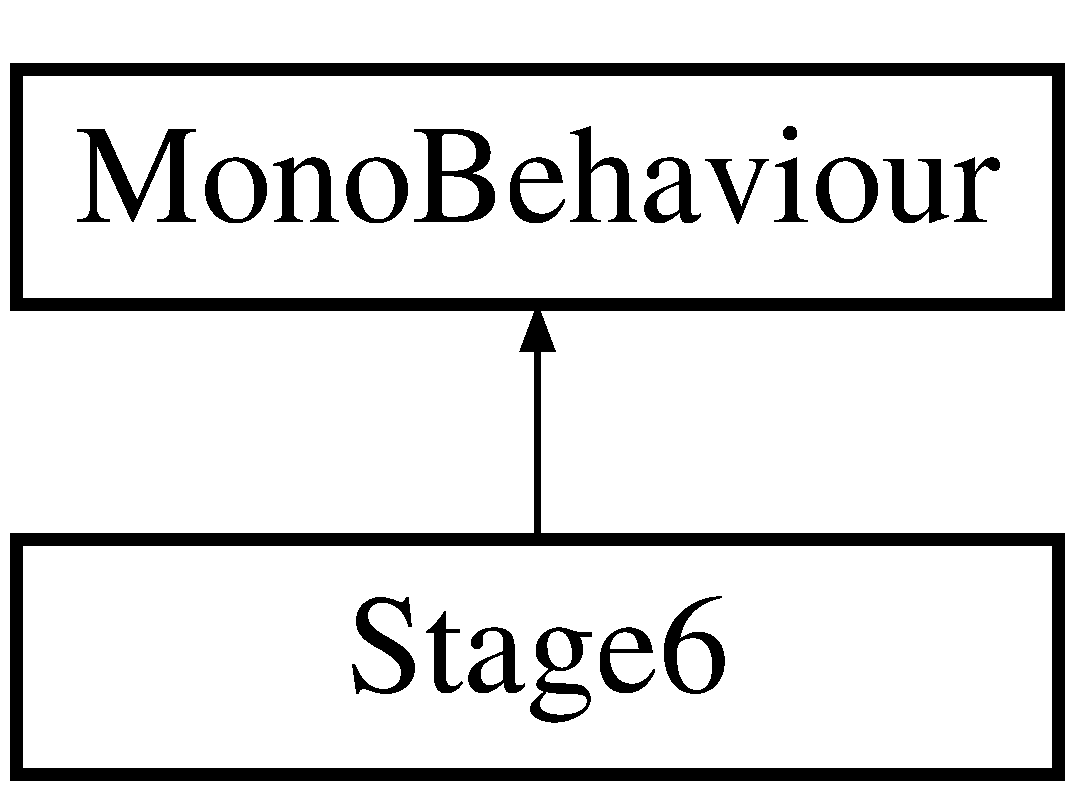
\includegraphics[height=2.000000cm]{class_stage6}
\end{center}
\end{figure}
\subsection*{Public Member Functions}
\begin{DoxyCompactItemize}
\item 
void \mbox{\hyperlink{class_stage6_a4c5fdae8e6d256d005e1ce12e313274c}{Notify\+Target\+Hit}} ()
\begin{DoxyCompactList}\small\item\em Is an event that keeps track of targets that are hit. If all targets are hit, calls end stage. \end{DoxyCompactList}\end{DoxyCompactItemize}
\subsection*{Static Public Attributes}
\begin{DoxyCompactItemize}
\item 
static \mbox{\hyperlink{class_stage6}{Stage6}} \mbox{\hyperlink{class_stage6_a4cf6e74a5141662ead48cd8099da2c08}{s\+\_\+\+Instance}} = null
\end{DoxyCompactItemize}
\subsection*{Private Member Functions}
\begin{DoxyCompactItemize}
\item 
void \mbox{\hyperlink{class_stage6_a0b1886eba20acc62966ff105e1ea51ed}{Start}} ()
\item 
void \mbox{\hyperlink{class_stage6_af13c178e81408130bc3178d88892fbef}{On\+Enable}} ()
\item 
void \mbox{\hyperlink{class_stage6_a2482ff2ad4b567c6c7308e7623ed2edd}{On\+Disable}} ()
\item 
void \mbox{\hyperlink{class_stage6_aad2cee8912a53eeb0f784e82a3a4e484}{Run}} ()
\begin{DoxyCompactList}\small\item\em Controls the flow of the scene. \end{DoxyCompactList}\item 
I\+Enumerator \mbox{\hyperlink{class_stage6_a5270b2b7fdc0958c4a9660f3528e2ebe}{Show\+Targets}} ()
\begin{DoxyCompactList}\small\item\em Generate all three targets. \end{DoxyCompactList}\item 
I\+Enumerator \mbox{\hyperlink{class_stage6_a1b5fa30c896fa0572746a20b6b3ebf71}{End\+Stage}} ()
\end{DoxyCompactItemize}
\subsection*{Private Attributes}
\begin{DoxyCompactItemize}
\item 
\mbox{\hyperlink{class_intro_session_manager}{Intro\+Session\+Manager}} \mbox{\hyperlink{class_stage6_ac4c230082e1cedefe1fee939af37addf}{m\+\_\+\+Manager}}
\item 
Game\+Object \mbox{\hyperlink{class_stage6_a48fe2476a0487b858be72ff53c6cddf7}{m\+\_\+\+Target1}}
\item 
Game\+Object \mbox{\hyperlink{class_stage6_a1756b8683311b102151c8307a2ac3055}{m\+\_\+\+Target2}}
\item 
Game\+Object \mbox{\hyperlink{class_stage6_ae64ded8ee411b39e0f939cf98bea940b}{m\+\_\+\+Target3}}
\item 
\mbox{\hyperlink{class_dialogue}{Dialogue}} \mbox{\hyperlink{class_stage6_a56acf5cd644988878b80fa187239f1fc}{m\+\_\+\+Dialogue\+Instructions}}
\item 
int \mbox{\hyperlink{class_stage6_a5453b72c92f4f68eba7675f26be39f59}{m\+\_\+\+Targets\+Alive}} = 3
\end{DoxyCompactItemize}


\subsection{Member Function Documentation}
\mbox{\Hypertarget{class_stage6_a1b5fa30c896fa0572746a20b6b3ebf71}\label{class_stage6_a1b5fa30c896fa0572746a20b6b3ebf71}} 
\index{Stage6@{Stage6}!End\+Stage@{End\+Stage}}
\index{End\+Stage@{End\+Stage}!Stage6@{Stage6}}
\subsubsection{\texorpdfstring{End\+Stage()}{EndStage()}}
{\footnotesize\ttfamily I\+Enumerator Stage6.\+End\+Stage (\begin{DoxyParamCaption}{ }\end{DoxyParamCaption})\hspace{0.3cm}{\ttfamily [private]}}





\begin{DoxyReturn}{Returns}

\end{DoxyReturn}
\mbox{\Hypertarget{class_stage6_a4c5fdae8e6d256d005e1ce12e313274c}\label{class_stage6_a4c5fdae8e6d256d005e1ce12e313274c}} 
\index{Stage6@{Stage6}!Notify\+Target\+Hit@{Notify\+Target\+Hit}}
\index{Notify\+Target\+Hit@{Notify\+Target\+Hit}!Stage6@{Stage6}}
\subsubsection{\texorpdfstring{Notify\+Target\+Hit()}{NotifyTargetHit()}}
{\footnotesize\ttfamily void Stage6.\+Notify\+Target\+Hit (\begin{DoxyParamCaption}{ }\end{DoxyParamCaption})}



Is an event that keeps track of targets that are hit. If all targets are hit, calls end stage. 

\mbox{\Hypertarget{class_stage6_a2482ff2ad4b567c6c7308e7623ed2edd}\label{class_stage6_a2482ff2ad4b567c6c7308e7623ed2edd}} 
\index{Stage6@{Stage6}!On\+Disable@{On\+Disable}}
\index{On\+Disable@{On\+Disable}!Stage6@{Stage6}}
\subsubsection{\texorpdfstring{On\+Disable()}{OnDisable()}}
{\footnotesize\ttfamily void Stage6.\+On\+Disable (\begin{DoxyParamCaption}{ }\end{DoxyParamCaption})\hspace{0.3cm}{\ttfamily [private]}}

\mbox{\Hypertarget{class_stage6_af13c178e81408130bc3178d88892fbef}\label{class_stage6_af13c178e81408130bc3178d88892fbef}} 
\index{Stage6@{Stage6}!On\+Enable@{On\+Enable}}
\index{On\+Enable@{On\+Enable}!Stage6@{Stage6}}
\subsubsection{\texorpdfstring{On\+Enable()}{OnEnable()}}
{\footnotesize\ttfamily void Stage6.\+On\+Enable (\begin{DoxyParamCaption}{ }\end{DoxyParamCaption})\hspace{0.3cm}{\ttfamily [private]}}

\mbox{\Hypertarget{class_stage6_aad2cee8912a53eeb0f784e82a3a4e484}\label{class_stage6_aad2cee8912a53eeb0f784e82a3a4e484}} 
\index{Stage6@{Stage6}!Run@{Run}}
\index{Run@{Run}!Stage6@{Stage6}}
\subsubsection{\texorpdfstring{Run()}{Run()}}
{\footnotesize\ttfamily void Stage6.\+Run (\begin{DoxyParamCaption}{ }\end{DoxyParamCaption})\hspace{0.3cm}{\ttfamily [private]}}



Controls the flow of the scene. 

\begin{DoxyReturn}{Returns}
A reference to the coroutine
\end{DoxyReturn}
\mbox{\Hypertarget{class_stage6_a5270b2b7fdc0958c4a9660f3528e2ebe}\label{class_stage6_a5270b2b7fdc0958c4a9660f3528e2ebe}} 
\index{Stage6@{Stage6}!Show\+Targets@{Show\+Targets}}
\index{Show\+Targets@{Show\+Targets}!Stage6@{Stage6}}
\subsubsection{\texorpdfstring{Show\+Targets()}{ShowTargets()}}
{\footnotesize\ttfamily I\+Enumerator Stage6.\+Show\+Targets (\begin{DoxyParamCaption}{ }\end{DoxyParamCaption})\hspace{0.3cm}{\ttfamily [private]}}



Generate all three targets. 

Returns I\+Enumerator Coroutine

\begin{DoxyReturn}{Returns}
I\+Enumerator Coroutine
\end{DoxyReturn}
\mbox{\Hypertarget{class_stage6_a0b1886eba20acc62966ff105e1ea51ed}\label{class_stage6_a0b1886eba20acc62966ff105e1ea51ed}} 
\index{Stage6@{Stage6}!Start@{Start}}
\index{Start@{Start}!Stage6@{Stage6}}
\subsubsection{\texorpdfstring{Start()}{Start()}}
{\footnotesize\ttfamily void Stage6.\+Start (\begin{DoxyParamCaption}{ }\end{DoxyParamCaption})\hspace{0.3cm}{\ttfamily [private]}}



\subsection{Member Data Documentation}
\mbox{\Hypertarget{class_stage6_a56acf5cd644988878b80fa187239f1fc}\label{class_stage6_a56acf5cd644988878b80fa187239f1fc}} 
\index{Stage6@{Stage6}!m\+\_\+\+Dialogue\+Instructions@{m\+\_\+\+Dialogue\+Instructions}}
\index{m\+\_\+\+Dialogue\+Instructions@{m\+\_\+\+Dialogue\+Instructions}!Stage6@{Stage6}}
\subsubsection{\texorpdfstring{m\+\_\+\+Dialogue\+Instructions}{m\_DialogueInstructions}}
{\footnotesize\ttfamily \mbox{\hyperlink{class_dialogue}{Dialogue}} Stage6.\+m\+\_\+\+Dialogue\+Instructions\hspace{0.3cm}{\ttfamily [private]}}

\mbox{\Hypertarget{class_stage6_ac4c230082e1cedefe1fee939af37addf}\label{class_stage6_ac4c230082e1cedefe1fee939af37addf}} 
\index{Stage6@{Stage6}!m\+\_\+\+Manager@{m\+\_\+\+Manager}}
\index{m\+\_\+\+Manager@{m\+\_\+\+Manager}!Stage6@{Stage6}}
\subsubsection{\texorpdfstring{m\+\_\+\+Manager}{m\_Manager}}
{\footnotesize\ttfamily \mbox{\hyperlink{class_intro_session_manager}{Intro\+Session\+Manager}} Stage6.\+m\+\_\+\+Manager\hspace{0.3cm}{\ttfamily [private]}}

\mbox{\Hypertarget{class_stage6_a48fe2476a0487b858be72ff53c6cddf7}\label{class_stage6_a48fe2476a0487b858be72ff53c6cddf7}} 
\index{Stage6@{Stage6}!m\+\_\+\+Target1@{m\+\_\+\+Target1}}
\index{m\+\_\+\+Target1@{m\+\_\+\+Target1}!Stage6@{Stage6}}
\subsubsection{\texorpdfstring{m\+\_\+\+Target1}{m\_Target1}}
{\footnotesize\ttfamily Game\+Object Stage6.\+m\+\_\+\+Target1\hspace{0.3cm}{\ttfamily [private]}}

\mbox{\Hypertarget{class_stage6_a1756b8683311b102151c8307a2ac3055}\label{class_stage6_a1756b8683311b102151c8307a2ac3055}} 
\index{Stage6@{Stage6}!m\+\_\+\+Target2@{m\+\_\+\+Target2}}
\index{m\+\_\+\+Target2@{m\+\_\+\+Target2}!Stage6@{Stage6}}
\subsubsection{\texorpdfstring{m\+\_\+\+Target2}{m\_Target2}}
{\footnotesize\ttfamily Game\+Object Stage6.\+m\+\_\+\+Target2\hspace{0.3cm}{\ttfamily [private]}}

\mbox{\Hypertarget{class_stage6_ae64ded8ee411b39e0f939cf98bea940b}\label{class_stage6_ae64ded8ee411b39e0f939cf98bea940b}} 
\index{Stage6@{Stage6}!m\+\_\+\+Target3@{m\+\_\+\+Target3}}
\index{m\+\_\+\+Target3@{m\+\_\+\+Target3}!Stage6@{Stage6}}
\subsubsection{\texorpdfstring{m\+\_\+\+Target3}{m\_Target3}}
{\footnotesize\ttfamily Game\+Object Stage6.\+m\+\_\+\+Target3\hspace{0.3cm}{\ttfamily [private]}}

\mbox{\Hypertarget{class_stage6_a5453b72c92f4f68eba7675f26be39f59}\label{class_stage6_a5453b72c92f4f68eba7675f26be39f59}} 
\index{Stage6@{Stage6}!m\+\_\+\+Targets\+Alive@{m\+\_\+\+Targets\+Alive}}
\index{m\+\_\+\+Targets\+Alive@{m\+\_\+\+Targets\+Alive}!Stage6@{Stage6}}
\subsubsection{\texorpdfstring{m\+\_\+\+Targets\+Alive}{m\_TargetsAlive}}
{\footnotesize\ttfamily int Stage6.\+m\+\_\+\+Targets\+Alive = 3\hspace{0.3cm}{\ttfamily [private]}}

\mbox{\Hypertarget{class_stage6_a4cf6e74a5141662ead48cd8099da2c08}\label{class_stage6_a4cf6e74a5141662ead48cd8099da2c08}} 
\index{Stage6@{Stage6}!s\+\_\+\+Instance@{s\+\_\+\+Instance}}
\index{s\+\_\+\+Instance@{s\+\_\+\+Instance}!Stage6@{Stage6}}
\subsubsection{\texorpdfstring{s\+\_\+\+Instance}{s\_Instance}}
{\footnotesize\ttfamily \mbox{\hyperlink{class_stage6}{Stage6}} Stage6.\+s\+\_\+\+Instance = null\hspace{0.3cm}{\ttfamily [static]}}



The documentation for this class was generated from the following file\+:\begin{DoxyCompactItemize}
\item 
\mbox{\hyperlink{_stage6_8cs}{Stage6.\+cs}}\end{DoxyCompactItemize}

\hypertarget{class_target}{}\section{Target Class Reference}
\label{class_target}\index{Target@{Target}}


Class is designed to be used on the targets in Scene6. They have a voxel effect when they are hit by the ball.  


Inheritance diagram for Target\+:\begin{figure}[H]
\begin{center}
\leavevmode
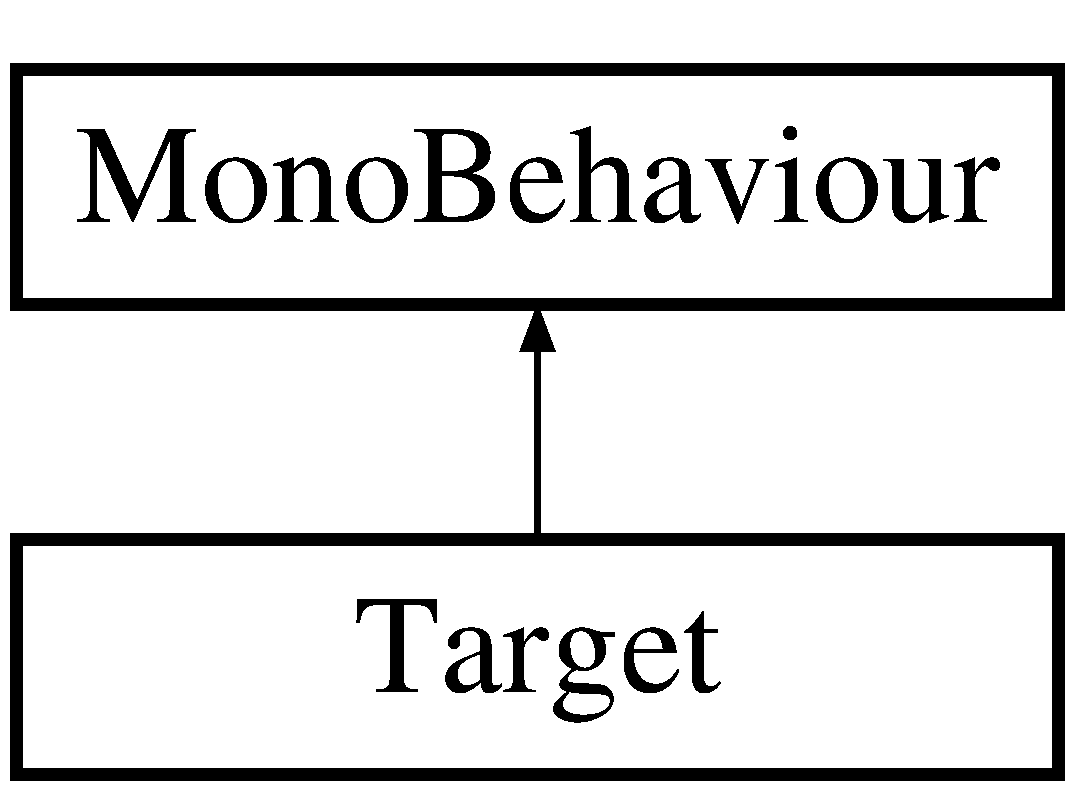
\includegraphics[height=2.000000cm]{class_target}
\end{center}
\end{figure}
\subsection*{Public Member Functions}
\begin{DoxyCompactItemize}
\item 
delegate void \mbox{\hyperlink{class_target_a4f2a0b66fecc85bdcf301cc9ab926898}{Ball\+Hit\+Target}} ()
\end{DoxyCompactItemize}
\subsection*{Events}
\begin{DoxyCompactItemize}
\item 
static \mbox{\hyperlink{class_target_a4f2a0b66fecc85bdcf301cc9ab926898}{Ball\+Hit\+Target}} \mbox{\hyperlink{class_target_aa54347b745ba5f74774bda61839cce75}{e\+\_\+\+Ball\+Hit\+The\+Target}}
\end{DoxyCompactItemize}
\subsection*{Private Member Functions}
\begin{DoxyCompactItemize}
\item 
void \mbox{\hyperlink{class_target_a0f01237749302a315f5f9427524ac45a}{Start}} ()
\item 
void \mbox{\hyperlink{class_target_adac88a907571e0494bbafc363236a84e}{On\+Trigger\+Enter}} (Collider collider)
\item 
I\+Enumerator \mbox{\hyperlink{class_target_af48513275b10a25477fb07f499a4b596}{Target\+Hit}} ()
\begin{DoxyCompactList}\small\item\em Once the target gets hit, wait 2.\+5 seconds to allow the voxels to spread out, then turn gravity on for each one and let them fall. \end{DoxyCompactList}\end{DoxyCompactItemize}
\subsection*{Private Attributes}
\begin{DoxyCompactItemize}
\item 
Rigidbody \mbox{[}$\,$\mbox{]} \mbox{\hyperlink{class_target_a570a932db2872d5f0d00656f038c2f21}{m\+\_\+children\+Rigid\+Bodies}}
\item 
bool \mbox{\hyperlink{class_target_abfdb205d5c2872d5d983b4e617eb5e40}{m\+\_\+\+Target\+Hit}}
\end{DoxyCompactItemize}


\subsection{Detailed Description}
Class is designed to be used on the targets in Scene6. They have a voxel effect when they are hit by the ball. 



\subsection{Member Function Documentation}
\mbox{\Hypertarget{class_target_a4f2a0b66fecc85bdcf301cc9ab926898}\label{class_target_a4f2a0b66fecc85bdcf301cc9ab926898}} 
\index{Target@{Target}!Ball\+Hit\+Target@{Ball\+Hit\+Target}}
\index{Ball\+Hit\+Target@{Ball\+Hit\+Target}!Target@{Target}}
\subsubsection{\texorpdfstring{Ball\+Hit\+Target()}{BallHitTarget()}}
{\footnotesize\ttfamily delegate void Target.\+Ball\+Hit\+Target (\begin{DoxyParamCaption}{ }\end{DoxyParamCaption})}

\mbox{\Hypertarget{class_target_adac88a907571e0494bbafc363236a84e}\label{class_target_adac88a907571e0494bbafc363236a84e}} 
\index{Target@{Target}!On\+Trigger\+Enter@{On\+Trigger\+Enter}}
\index{On\+Trigger\+Enter@{On\+Trigger\+Enter}!Target@{Target}}
\subsubsection{\texorpdfstring{On\+Trigger\+Enter()}{OnTriggerEnter()}}
{\footnotesize\ttfamily void Target.\+On\+Trigger\+Enter (\begin{DoxyParamCaption}\item[{Collider}]{collider }\end{DoxyParamCaption})\hspace{0.3cm}{\ttfamily [private]}}

\mbox{\Hypertarget{class_target_a0f01237749302a315f5f9427524ac45a}\label{class_target_a0f01237749302a315f5f9427524ac45a}} 
\index{Target@{Target}!Start@{Start}}
\index{Start@{Start}!Target@{Target}}
\subsubsection{\texorpdfstring{Start()}{Start()}}
{\footnotesize\ttfamily void Target.\+Start (\begin{DoxyParamCaption}{ }\end{DoxyParamCaption})\hspace{0.3cm}{\ttfamily [private]}}

\mbox{\Hypertarget{class_target_af48513275b10a25477fb07f499a4b596}\label{class_target_af48513275b10a25477fb07f499a4b596}} 
\index{Target@{Target}!Target\+Hit@{Target\+Hit}}
\index{Target\+Hit@{Target\+Hit}!Target@{Target}}
\subsubsection{\texorpdfstring{Target\+Hit()}{TargetHit()}}
{\footnotesize\ttfamily I\+Enumerator Target.\+Target\+Hit (\begin{DoxyParamCaption}{ }\end{DoxyParamCaption})\hspace{0.3cm}{\ttfamily [private]}}



Once the target gets hit, wait 2.\+5 seconds to allow the voxels to spread out, then turn gravity on for each one and let them fall. 

\begin{DoxyReturn}{Returns}
A reference to the coroutine
\end{DoxyReturn}


\subsection{Member Data Documentation}
\mbox{\Hypertarget{class_target_a570a932db2872d5f0d00656f038c2f21}\label{class_target_a570a932db2872d5f0d00656f038c2f21}} 
\index{Target@{Target}!m\+\_\+children\+Rigid\+Bodies@{m\+\_\+children\+Rigid\+Bodies}}
\index{m\+\_\+children\+Rigid\+Bodies@{m\+\_\+children\+Rigid\+Bodies}!Target@{Target}}
\subsubsection{\texorpdfstring{m\+\_\+children\+Rigid\+Bodies}{m\_childrenRigidBodies}}
{\footnotesize\ttfamily Rigidbody \mbox{[}$\,$\mbox{]} Target.\+m\+\_\+children\+Rigid\+Bodies\hspace{0.3cm}{\ttfamily [private]}}

\mbox{\Hypertarget{class_target_abfdb205d5c2872d5d983b4e617eb5e40}\label{class_target_abfdb205d5c2872d5d983b4e617eb5e40}} 
\index{Target@{Target}!m\+\_\+\+Target\+Hit@{m\+\_\+\+Target\+Hit}}
\index{m\+\_\+\+Target\+Hit@{m\+\_\+\+Target\+Hit}!Target@{Target}}
\subsubsection{\texorpdfstring{m\+\_\+\+Target\+Hit}{m\_TargetHit}}
{\footnotesize\ttfamily bool Target.\+m\+\_\+\+Target\+Hit\hspace{0.3cm}{\ttfamily [private]}}



\subsection{Event Documentation}
\mbox{\Hypertarget{class_target_aa54347b745ba5f74774bda61839cce75}\label{class_target_aa54347b745ba5f74774bda61839cce75}} 
\index{Target@{Target}!e\+\_\+\+Ball\+Hit\+The\+Target@{e\+\_\+\+Ball\+Hit\+The\+Target}}
\index{e\+\_\+\+Ball\+Hit\+The\+Target@{e\+\_\+\+Ball\+Hit\+The\+Target}!Target@{Target}}
\subsubsection{\texorpdfstring{e\+\_\+\+Ball\+Hit\+The\+Target}{e\_BallHitTheTarget}}
{\footnotesize\ttfamily \mbox{\hyperlink{class_target_a4f2a0b66fecc85bdcf301cc9ab926898}{Ball\+Hit\+Target}} Target.\+e\+\_\+\+Ball\+Hit\+The\+Target\hspace{0.3cm}{\ttfamily [static]}}



The documentation for this class was generated from the following file\+:\begin{DoxyCompactItemize}
\item 
\mbox{\hyperlink{_target_8cs}{Target.\+cs}}\end{DoxyCompactItemize}

\hypertarget{class_trigger_stage4}{}\section{Trigger\+Stage4 Class Reference}
\label{class_trigger_stage4}\index{Trigger\+Stage4@{Trigger\+Stage4}}


Class is designed for Scene4 to be listening for when an object is dropped through the doors  


Inheritance diagram for Trigger\+Stage4\+:\begin{figure}[H]
\begin{center}
\leavevmode
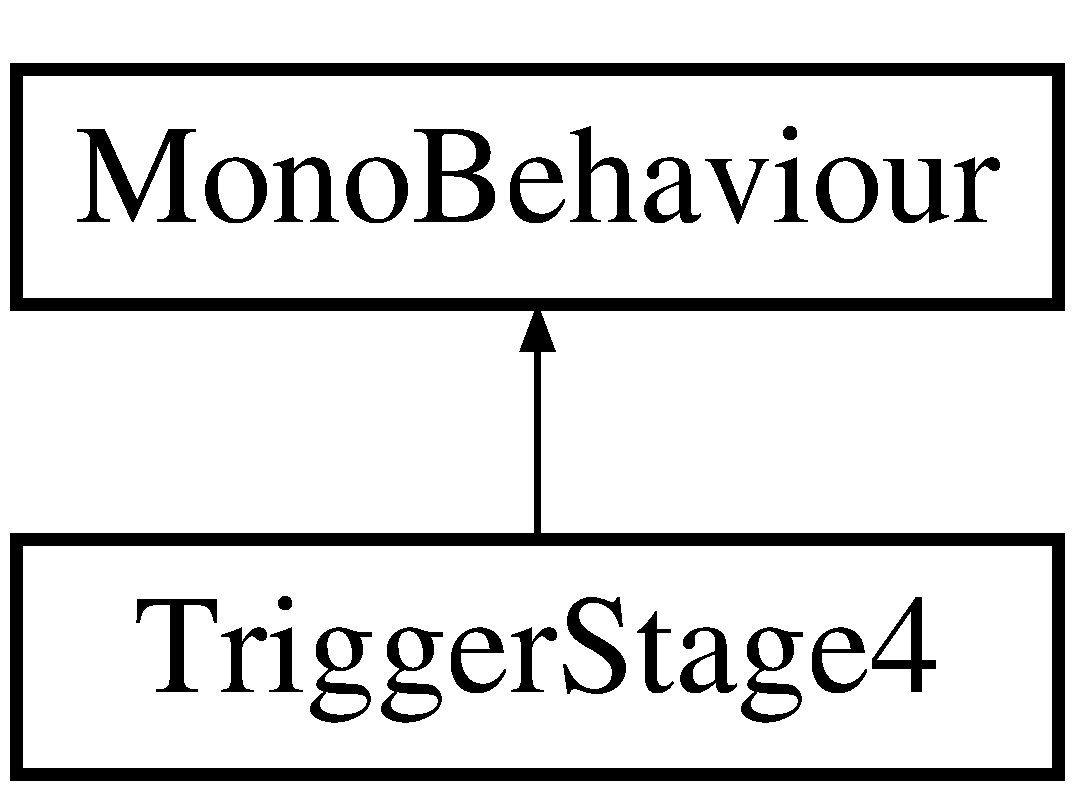
\includegraphics[height=2.000000cm]{class_trigger_stage4}
\end{center}
\end{figure}
\subsection*{Public Member Functions}
\begin{DoxyCompactItemize}
\item 
delegate void \mbox{\hyperlink{class_trigger_stage4_a9b09ff6aa89d24158570596dc578bc0a}{Stage4\+Trigger}} ()
\end{DoxyCompactItemize}
\subsection*{Events}
\begin{DoxyCompactItemize}
\item 
static \mbox{\hyperlink{class_trigger_stage4_a9b09ff6aa89d24158570596dc578bc0a}{Stage4\+Trigger}} \mbox{\hyperlink{class_trigger_stage4_ac33c360701aebd4eeefcc2c63bdb8b19}{e\+\_\+\+Stage4\+Triggered}}
\end{DoxyCompactItemize}
\subsection*{Private Member Functions}
\begin{DoxyCompactItemize}
\item 
void \mbox{\hyperlink{class_trigger_stage4_a75b1f3045df85b380a4eebeed44fe217}{On\+Trigger\+Enter}} (Collider other)
\end{DoxyCompactItemize}


\subsection{Detailed Description}
Class is designed for Scene4 to be listening for when an object is dropped through the doors 



\subsection{Member Function Documentation}
\mbox{\Hypertarget{class_trigger_stage4_a75b1f3045df85b380a4eebeed44fe217}\label{class_trigger_stage4_a75b1f3045df85b380a4eebeed44fe217}} 
\index{Trigger\+Stage4@{Trigger\+Stage4}!On\+Trigger\+Enter@{On\+Trigger\+Enter}}
\index{On\+Trigger\+Enter@{On\+Trigger\+Enter}!Trigger\+Stage4@{Trigger\+Stage4}}
\subsubsection{\texorpdfstring{On\+Trigger\+Enter()}{OnTriggerEnter()}}
{\footnotesize\ttfamily void Trigger\+Stage4.\+On\+Trigger\+Enter (\begin{DoxyParamCaption}\item[{Collider}]{other }\end{DoxyParamCaption})\hspace{0.3cm}{\ttfamily [private]}}

\mbox{\Hypertarget{class_trigger_stage4_a9b09ff6aa89d24158570596dc578bc0a}\label{class_trigger_stage4_a9b09ff6aa89d24158570596dc578bc0a}} 
\index{Trigger\+Stage4@{Trigger\+Stage4}!Stage4\+Trigger@{Stage4\+Trigger}}
\index{Stage4\+Trigger@{Stage4\+Trigger}!Trigger\+Stage4@{Trigger\+Stage4}}
\subsubsection{\texorpdfstring{Stage4\+Trigger()}{Stage4Trigger()}}
{\footnotesize\ttfamily delegate void Trigger\+Stage4.\+Stage4\+Trigger (\begin{DoxyParamCaption}{ }\end{DoxyParamCaption})}



\subsection{Event Documentation}
\mbox{\Hypertarget{class_trigger_stage4_ac33c360701aebd4eeefcc2c63bdb8b19}\label{class_trigger_stage4_ac33c360701aebd4eeefcc2c63bdb8b19}} 
\index{Trigger\+Stage4@{Trigger\+Stage4}!e\+\_\+\+Stage4\+Triggered@{e\+\_\+\+Stage4\+Triggered}}
\index{e\+\_\+\+Stage4\+Triggered@{e\+\_\+\+Stage4\+Triggered}!Trigger\+Stage4@{Trigger\+Stage4}}
\subsubsection{\texorpdfstring{e\+\_\+\+Stage4\+Triggered}{e\_Stage4Triggered}}
{\footnotesize\ttfamily \mbox{\hyperlink{class_trigger_stage4_a9b09ff6aa89d24158570596dc578bc0a}{Stage4\+Trigger}} Trigger\+Stage4.\+e\+\_\+\+Stage4\+Triggered\hspace{0.3cm}{\ttfamily [static]}}



The documentation for this class was generated from the following file\+:\begin{DoxyCompactItemize}
\item 
\mbox{\hyperlink{_trigger_stage4_8cs}{Trigger\+Stage4.\+cs}}\end{DoxyCompactItemize}

\hypertarget{class_v_r_standard_assets_1_1_utils_1_1_v_r_camera_u_i}{}\section{V\+R\+Standard\+Assets.\+Utils.\+V\+R\+Camera\+UI Class Reference}
\label{class_v_r_standard_assets_1_1_utils_1_1_v_r_camera_u_i}\index{V\+R\+Standard\+Assets.\+Utils.\+V\+R\+Camera\+UI@{V\+R\+Standard\+Assets.\+Utils.\+V\+R\+Camera\+UI}}
Inheritance diagram for V\+R\+Standard\+Assets.\+Utils.\+V\+R\+Camera\+UI\+:\begin{figure}[H]
\begin{center}
\leavevmode
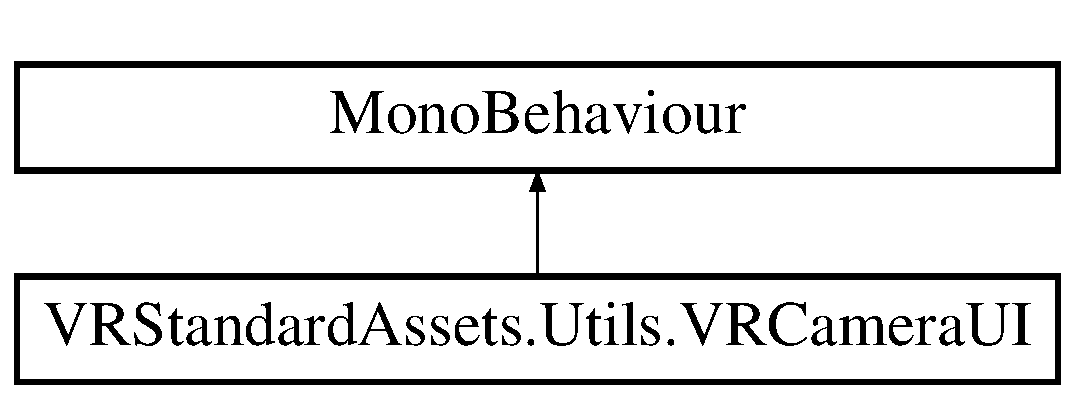
\includegraphics[height=2.000000cm]{class_v_r_standard_assets_1_1_utils_1_1_v_r_camera_u_i}
\end{center}
\end{figure}
\subsection*{Private Member Functions}
\begin{DoxyCompactItemize}
\item 
void \mbox{\hyperlink{class_v_r_standard_assets_1_1_utils_1_1_v_r_camera_u_i_a97c31c7ee563db0395bf6c970f0e88aa}{Awake}} ()
\end{DoxyCompactItemize}
\subsection*{Private Attributes}
\begin{DoxyCompactItemize}
\item 
Canvas \mbox{\hyperlink{class_v_r_standard_assets_1_1_utils_1_1_v_r_camera_u_i_afef7aad14b8afe269014143749aa2622}{m\+\_\+\+Canvas}}
\end{DoxyCompactItemize}


\subsection{Member Function Documentation}
\mbox{\Hypertarget{class_v_r_standard_assets_1_1_utils_1_1_v_r_camera_u_i_a97c31c7ee563db0395bf6c970f0e88aa}\label{class_v_r_standard_assets_1_1_utils_1_1_v_r_camera_u_i_a97c31c7ee563db0395bf6c970f0e88aa}} 
\index{V\+R\+Standard\+Assets\+::\+Utils\+::\+V\+R\+Camera\+UI@{V\+R\+Standard\+Assets\+::\+Utils\+::\+V\+R\+Camera\+UI}!Awake@{Awake}}
\index{Awake@{Awake}!V\+R\+Standard\+Assets\+::\+Utils\+::\+V\+R\+Camera\+UI@{V\+R\+Standard\+Assets\+::\+Utils\+::\+V\+R\+Camera\+UI}}
\subsubsection{\texorpdfstring{Awake()}{Awake()}}
{\footnotesize\ttfamily void V\+R\+Standard\+Assets.\+Utils.\+V\+R\+Camera\+U\+I.\+Awake (\begin{DoxyParamCaption}{ }\end{DoxyParamCaption})\hspace{0.3cm}{\ttfamily [private]}}



\subsection{Member Data Documentation}
\mbox{\Hypertarget{class_v_r_standard_assets_1_1_utils_1_1_v_r_camera_u_i_afef7aad14b8afe269014143749aa2622}\label{class_v_r_standard_assets_1_1_utils_1_1_v_r_camera_u_i_afef7aad14b8afe269014143749aa2622}} 
\index{V\+R\+Standard\+Assets\+::\+Utils\+::\+V\+R\+Camera\+UI@{V\+R\+Standard\+Assets\+::\+Utils\+::\+V\+R\+Camera\+UI}!m\+\_\+\+Canvas@{m\+\_\+\+Canvas}}
\index{m\+\_\+\+Canvas@{m\+\_\+\+Canvas}!V\+R\+Standard\+Assets\+::\+Utils\+::\+V\+R\+Camera\+UI@{V\+R\+Standard\+Assets\+::\+Utils\+::\+V\+R\+Camera\+UI}}
\subsubsection{\texorpdfstring{m\+\_\+\+Canvas}{m\_Canvas}}
{\footnotesize\ttfamily Canvas V\+R\+Standard\+Assets.\+Utils.\+V\+R\+Camera\+U\+I.\+m\+\_\+\+Canvas\hspace{0.3cm}{\ttfamily [private]}}



The documentation for this class was generated from the following file\+:\begin{DoxyCompactItemize}
\item 
\mbox{\hyperlink{_v_r_camera_u_i_8cs}{V\+R\+Camera\+U\+I.\+cs}}\end{DoxyCompactItemize}

\hypertarget{class_v_r_standard_assets_1_1_utils_1_1_v_r_device_manager}{}\section{V\+R\+Standard\+Assets.\+Utils.\+V\+R\+Device\+Manager Class Reference}
\label{class_v_r_standard_assets_1_1_utils_1_1_v_r_device_manager}\index{V\+R\+Standard\+Assets.\+Utils.\+V\+R\+Device\+Manager@{V\+R\+Standard\+Assets.\+Utils.\+V\+R\+Device\+Manager}}
Inheritance diagram for V\+R\+Standard\+Assets.\+Utils.\+V\+R\+Device\+Manager\+:\begin{figure}[H]
\begin{center}
\leavevmode
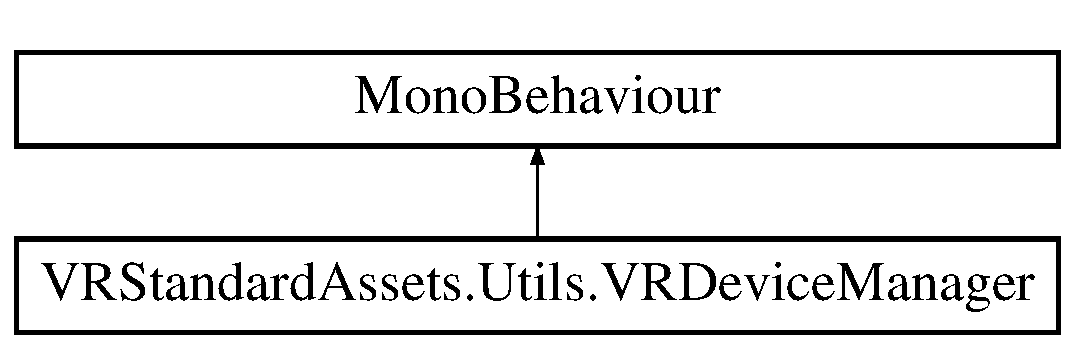
\includegraphics[height=2.000000cm]{class_v_r_standard_assets_1_1_utils_1_1_v_r_device_manager}
\end{center}
\end{figure}
\subsection*{Properties}
\begin{DoxyCompactItemize}
\item 
static \mbox{\hyperlink{class_v_r_standard_assets_1_1_utils_1_1_v_r_device_manager}{V\+R\+Device\+Manager}} \mbox{\hyperlink{class_v_r_standard_assets_1_1_utils_1_1_v_r_device_manager_ae45832ea5dead7782321d7e3ae25992f}{Instance}}\hspace{0.3cm}{\ttfamily  \mbox{[}get\mbox{]}}
\end{DoxyCompactItemize}
\subsection*{Private Member Functions}
\begin{DoxyCompactItemize}
\item 
void \mbox{\hyperlink{class_v_r_standard_assets_1_1_utils_1_1_v_r_device_manager_a8ad85381877fb58fff146d9223e69584}{Awake}} ()
\end{DoxyCompactItemize}
\subsection*{Private Attributes}
\begin{DoxyCompactItemize}
\item 
float \mbox{\hyperlink{class_v_r_standard_assets_1_1_utils_1_1_v_r_device_manager_a6e9a73ee11c79c9adeca5d5246fc03d3}{m\+\_\+\+Render\+Scale}} = 1.\+4f
\end{DoxyCompactItemize}
\subsection*{Static Private Attributes}
\begin{DoxyCompactItemize}
\item 
static \mbox{\hyperlink{class_v_r_standard_assets_1_1_utils_1_1_v_r_device_manager}{V\+R\+Device\+Manager}} \mbox{\hyperlink{class_v_r_standard_assets_1_1_utils_1_1_v_r_device_manager_a32f675f10d731bb23f266c189aae2153}{s\+\_\+\+Instance}}
\end{DoxyCompactItemize}


\subsection{Member Function Documentation}
\mbox{\Hypertarget{class_v_r_standard_assets_1_1_utils_1_1_v_r_device_manager_a8ad85381877fb58fff146d9223e69584}\label{class_v_r_standard_assets_1_1_utils_1_1_v_r_device_manager_a8ad85381877fb58fff146d9223e69584}} 
\index{V\+R\+Standard\+Assets\+::\+Utils\+::\+V\+R\+Device\+Manager@{V\+R\+Standard\+Assets\+::\+Utils\+::\+V\+R\+Device\+Manager}!Awake@{Awake}}
\index{Awake@{Awake}!V\+R\+Standard\+Assets\+::\+Utils\+::\+V\+R\+Device\+Manager@{V\+R\+Standard\+Assets\+::\+Utils\+::\+V\+R\+Device\+Manager}}
\subsubsection{\texorpdfstring{Awake()}{Awake()}}
{\footnotesize\ttfamily void V\+R\+Standard\+Assets.\+Utils.\+V\+R\+Device\+Manager.\+Awake (\begin{DoxyParamCaption}{ }\end{DoxyParamCaption})\hspace{0.3cm}{\ttfamily [private]}}



\subsection{Member Data Documentation}
\mbox{\Hypertarget{class_v_r_standard_assets_1_1_utils_1_1_v_r_device_manager_a6e9a73ee11c79c9adeca5d5246fc03d3}\label{class_v_r_standard_assets_1_1_utils_1_1_v_r_device_manager_a6e9a73ee11c79c9adeca5d5246fc03d3}} 
\index{V\+R\+Standard\+Assets\+::\+Utils\+::\+V\+R\+Device\+Manager@{V\+R\+Standard\+Assets\+::\+Utils\+::\+V\+R\+Device\+Manager}!m\+\_\+\+Render\+Scale@{m\+\_\+\+Render\+Scale}}
\index{m\+\_\+\+Render\+Scale@{m\+\_\+\+Render\+Scale}!V\+R\+Standard\+Assets\+::\+Utils\+::\+V\+R\+Device\+Manager@{V\+R\+Standard\+Assets\+::\+Utils\+::\+V\+R\+Device\+Manager}}
\subsubsection{\texorpdfstring{m\+\_\+\+Render\+Scale}{m\_RenderScale}}
{\footnotesize\ttfamily float V\+R\+Standard\+Assets.\+Utils.\+V\+R\+Device\+Manager.\+m\+\_\+\+Render\+Scale = 1.\+4f\hspace{0.3cm}{\ttfamily [private]}}

\mbox{\Hypertarget{class_v_r_standard_assets_1_1_utils_1_1_v_r_device_manager_a32f675f10d731bb23f266c189aae2153}\label{class_v_r_standard_assets_1_1_utils_1_1_v_r_device_manager_a32f675f10d731bb23f266c189aae2153}} 
\index{V\+R\+Standard\+Assets\+::\+Utils\+::\+V\+R\+Device\+Manager@{V\+R\+Standard\+Assets\+::\+Utils\+::\+V\+R\+Device\+Manager}!s\+\_\+\+Instance@{s\+\_\+\+Instance}}
\index{s\+\_\+\+Instance@{s\+\_\+\+Instance}!V\+R\+Standard\+Assets\+::\+Utils\+::\+V\+R\+Device\+Manager@{V\+R\+Standard\+Assets\+::\+Utils\+::\+V\+R\+Device\+Manager}}
\subsubsection{\texorpdfstring{s\+\_\+\+Instance}{s\_Instance}}
{\footnotesize\ttfamily \mbox{\hyperlink{class_v_r_standard_assets_1_1_utils_1_1_v_r_device_manager}{V\+R\+Device\+Manager}} V\+R\+Standard\+Assets.\+Utils.\+V\+R\+Device\+Manager.\+s\+\_\+\+Instance\hspace{0.3cm}{\ttfamily [static]}, {\ttfamily [private]}}



\subsection{Property Documentation}
\mbox{\Hypertarget{class_v_r_standard_assets_1_1_utils_1_1_v_r_device_manager_ae45832ea5dead7782321d7e3ae25992f}\label{class_v_r_standard_assets_1_1_utils_1_1_v_r_device_manager_ae45832ea5dead7782321d7e3ae25992f}} 
\index{V\+R\+Standard\+Assets\+::\+Utils\+::\+V\+R\+Device\+Manager@{V\+R\+Standard\+Assets\+::\+Utils\+::\+V\+R\+Device\+Manager}!Instance@{Instance}}
\index{Instance@{Instance}!V\+R\+Standard\+Assets\+::\+Utils\+::\+V\+R\+Device\+Manager@{V\+R\+Standard\+Assets\+::\+Utils\+::\+V\+R\+Device\+Manager}}
\subsubsection{\texorpdfstring{Instance}{Instance}}
{\footnotesize\ttfamily \mbox{\hyperlink{class_v_r_standard_assets_1_1_utils_1_1_v_r_device_manager}{V\+R\+Device\+Manager}} V\+R\+Standard\+Assets.\+Utils.\+V\+R\+Device\+Manager.\+Instance\hspace{0.3cm}{\ttfamily [static]}, {\ttfamily [get]}}



The documentation for this class was generated from the following file\+:\begin{DoxyCompactItemize}
\item 
\mbox{\hyperlink{_v_r_device_manager_8cs}{V\+R\+Device\+Manager.\+cs}}\end{DoxyCompactItemize}

\hypertarget{class_v_r_standard_assets_1_1_utils_1_1_v_r_input}{}\section{V\+R\+Standard\+Assets.\+Utils.\+V\+R\+Input Class Reference}
\label{class_v_r_standard_assets_1_1_utils_1_1_v_r_input}\index{V\+R\+Standard\+Assets.\+Utils.\+V\+R\+Input@{V\+R\+Standard\+Assets.\+Utils.\+V\+R\+Input}}
Inheritance diagram for V\+R\+Standard\+Assets.\+Utils.\+V\+R\+Input\+:\begin{figure}[H]
\begin{center}
\leavevmode
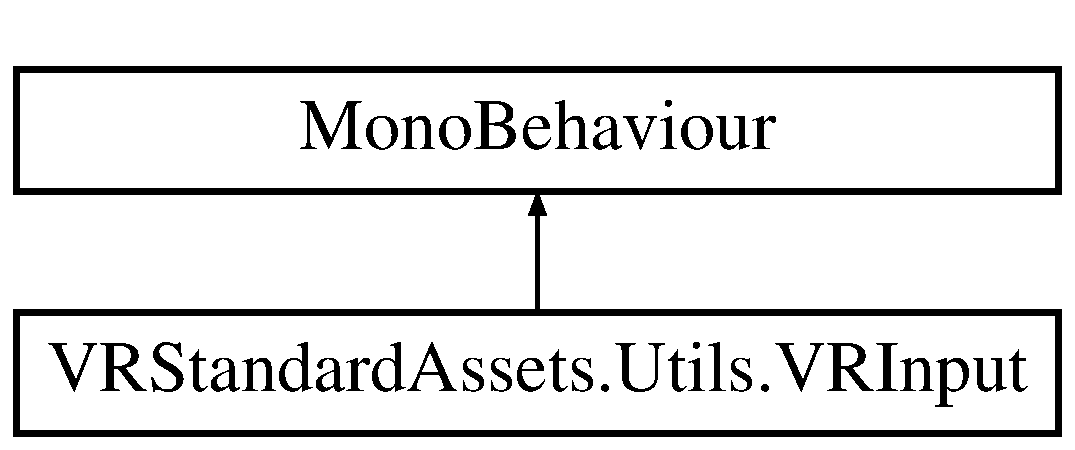
\includegraphics[height=2.000000cm]{class_v_r_standard_assets_1_1_utils_1_1_v_r_input}
\end{center}
\end{figure}
\subsection*{Public Types}
\begin{DoxyCompactItemize}
\item 
enum \mbox{\hyperlink{class_v_r_standard_assets_1_1_utils_1_1_v_r_input_a2ea76769ddd926c08921d6684d332538}{Swipe\+Direction}} \{ \newline
\mbox{\hyperlink{class_v_r_standard_assets_1_1_utils_1_1_v_r_input_a2ea76769ddd926c08921d6684d332538ab50339a10e1de285ac99d4c3990b8693}{Swipe\+Direction.\+N\+O\+NE}}, 
\mbox{\hyperlink{class_v_r_standard_assets_1_1_utils_1_1_v_r_input_a2ea76769ddd926c08921d6684d332538afbaedde498cdead4f2780217646e9ba1}{Swipe\+Direction.\+UP}}, 
\mbox{\hyperlink{class_v_r_standard_assets_1_1_utils_1_1_v_r_input_a2ea76769ddd926c08921d6684d332538ac4e0e4e3118472beeb2ae75827450f1f}{Swipe\+Direction.\+D\+O\+WN}}, 
\mbox{\hyperlink{class_v_r_standard_assets_1_1_utils_1_1_v_r_input_a2ea76769ddd926c08921d6684d332538a684d325a7303f52e64011467ff5c5758}{Swipe\+Direction.\+L\+E\+FT}}, 
\newline
\mbox{\hyperlink{class_v_r_standard_assets_1_1_utils_1_1_v_r_input_a2ea76769ddd926c08921d6684d332538a21507b40c80068eda19865706fdc2403}{Swipe\+Direction.\+R\+I\+G\+HT}}
 \}
\end{DoxyCompactItemize}
\subsection*{Properties}
\begin{DoxyCompactItemize}
\item 
float \mbox{\hyperlink{class_v_r_standard_assets_1_1_utils_1_1_v_r_input_a57b4846b4cc61b8042ad0d2be88905a5}{Double\+Click\+Time}}\hspace{0.3cm}{\ttfamily  \mbox{[}get\mbox{]}}
\end{DoxyCompactItemize}
\subsection*{Events}
\begin{DoxyCompactItemize}
\item 
Action$<$ \mbox{\hyperlink{class_v_r_standard_assets_1_1_utils_1_1_v_r_input_a2ea76769ddd926c08921d6684d332538}{Swipe\+Direction}} $>$ \mbox{\hyperlink{class_v_r_standard_assets_1_1_utils_1_1_v_r_input_a514bc58871fa0f6dbe7906a210baedb4}{On\+Swipe}}
\item 
Action \mbox{\hyperlink{class_v_r_standard_assets_1_1_utils_1_1_v_r_input_aef5ca345e6f0931cbd27794bec5b8625}{On\+Click}}
\item 
Action \mbox{\hyperlink{class_v_r_standard_assets_1_1_utils_1_1_v_r_input_a4b0437e852ada367a1a4a7316b8afefe}{On\+Down}}
\item 
Action \mbox{\hyperlink{class_v_r_standard_assets_1_1_utils_1_1_v_r_input_a96e97c6dceae4e43aee27d3fbe4ee29a}{On\+Up}}
\item 
Action \mbox{\hyperlink{class_v_r_standard_assets_1_1_utils_1_1_v_r_input_a6114e4322f194534fe265b4242b534a1}{On\+Double\+Click}}
\item 
Action \mbox{\hyperlink{class_v_r_standard_assets_1_1_utils_1_1_v_r_input_a6b6478f12f71a065e2448de07bf44dfa}{On\+Cancel}}
\end{DoxyCompactItemize}
\subsection*{Private Member Functions}
\begin{DoxyCompactItemize}
\item 
void \mbox{\hyperlink{class_v_r_standard_assets_1_1_utils_1_1_v_r_input_a811fbf86569a35075b16df5e8e51522d}{Update}} ()
\item 
void \mbox{\hyperlink{class_v_r_standard_assets_1_1_utils_1_1_v_r_input_a194207fffdfb2f9183be96dc3280a8a5}{Check\+Input}} ()
\item 
\mbox{\hyperlink{class_v_r_standard_assets_1_1_utils_1_1_v_r_input_a2ea76769ddd926c08921d6684d332538}{Swipe\+Direction}} \mbox{\hyperlink{class_v_r_standard_assets_1_1_utils_1_1_v_r_input_a7a537a50a8bcd6943bc0440a235de87c}{Detect\+Swipe}} ()
\item 
\mbox{\hyperlink{class_v_r_standard_assets_1_1_utils_1_1_v_r_input_a2ea76769ddd926c08921d6684d332538}{Swipe\+Direction}} \mbox{\hyperlink{class_v_r_standard_assets_1_1_utils_1_1_v_r_input_a2d38977aebcf43eed5d8a7d61a650b8c}{Detect\+Keyboard\+Emulated\+Swipe}} ()
\item 
void \mbox{\hyperlink{class_v_r_standard_assets_1_1_utils_1_1_v_r_input_aae660444b23ba964269c46576e3e15c0}{On\+Destroy}} ()
\end{DoxyCompactItemize}
\subsection*{Private Attributes}
\begin{DoxyCompactItemize}
\item 
float \mbox{\hyperlink{class_v_r_standard_assets_1_1_utils_1_1_v_r_input_ac9872d104ac983e43ab3a77057807676}{m\+\_\+\+Double\+Click\+Time}} = 0.\+3f
\item 
float \mbox{\hyperlink{class_v_r_standard_assets_1_1_utils_1_1_v_r_input_a07546688dd3d1f83aa1862853c0f6501}{m\+\_\+\+Swipe\+Width}} = 0.\+3f
\item 
Vector2 \mbox{\hyperlink{class_v_r_standard_assets_1_1_utils_1_1_v_r_input_a7a03517dfaeed90e07863ec2562704aa}{m\+\_\+\+Mouse\+Down\+Position}}
\item 
Vector2 \mbox{\hyperlink{class_v_r_standard_assets_1_1_utils_1_1_v_r_input_aec977a8bd3fb2b1821dac01ddb0a33ef}{m\+\_\+\+Mouse\+Up\+Position}}
\item 
float \mbox{\hyperlink{class_v_r_standard_assets_1_1_utils_1_1_v_r_input_a839d56368fff7606c43d65ccba8a769e}{m\+\_\+\+Last\+Mouse\+Up\+Time}}
\item 
float \mbox{\hyperlink{class_v_r_standard_assets_1_1_utils_1_1_v_r_input_ad0b9f0689c1e4813c70dd6326783dcd7}{m\+\_\+\+Last\+Horizontal\+Value}}
\item 
float \mbox{\hyperlink{class_v_r_standard_assets_1_1_utils_1_1_v_r_input_aa92baa6f51fd201eb34d98298c8bb4bc}{m\+\_\+\+Last\+Vertical\+Value}}
\end{DoxyCompactItemize}


\subsection{Member Enumeration Documentation}
\mbox{\Hypertarget{class_v_r_standard_assets_1_1_utils_1_1_v_r_input_a2ea76769ddd926c08921d6684d332538}\label{class_v_r_standard_assets_1_1_utils_1_1_v_r_input_a2ea76769ddd926c08921d6684d332538}} 
\index{V\+R\+Standard\+Assets\+::\+Utils\+::\+V\+R\+Input@{V\+R\+Standard\+Assets\+::\+Utils\+::\+V\+R\+Input}!Swipe\+Direction@{Swipe\+Direction}}
\index{Swipe\+Direction@{Swipe\+Direction}!V\+R\+Standard\+Assets\+::\+Utils\+::\+V\+R\+Input@{V\+R\+Standard\+Assets\+::\+Utils\+::\+V\+R\+Input}}
\subsubsection{\texorpdfstring{Swipe\+Direction}{SwipeDirection}}
{\footnotesize\ttfamily enum \mbox{\hyperlink{class_v_r_standard_assets_1_1_utils_1_1_v_r_input_a2ea76769ddd926c08921d6684d332538}{V\+R\+Standard\+Assets.\+Utils.\+V\+R\+Input.\+Swipe\+Direction}}\hspace{0.3cm}{\ttfamily [strong]}}

\begin{DoxyEnumFields}{Enumerator}
\raisebox{\heightof{T}}[0pt][0pt]{\index{N\+O\+NE@{N\+O\+NE}!V\+R\+Standard\+Assets\+::\+Utils\+::\+V\+R\+Input@{V\+R\+Standard\+Assets\+::\+Utils\+::\+V\+R\+Input}}\index{V\+R\+Standard\+Assets\+::\+Utils\+::\+V\+R\+Input@{V\+R\+Standard\+Assets\+::\+Utils\+::\+V\+R\+Input}!N\+O\+NE@{N\+O\+NE}}}\mbox{\Hypertarget{class_v_r_standard_assets_1_1_utils_1_1_v_r_input_a2ea76769ddd926c08921d6684d332538ab50339a10e1de285ac99d4c3990b8693}\label{class_v_r_standard_assets_1_1_utils_1_1_v_r_input_a2ea76769ddd926c08921d6684d332538ab50339a10e1de285ac99d4c3990b8693}} 
N\+O\+NE&\\
\hline

\raisebox{\heightof{T}}[0pt][0pt]{\index{UP@{UP}!V\+R\+Standard\+Assets\+::\+Utils\+::\+V\+R\+Input@{V\+R\+Standard\+Assets\+::\+Utils\+::\+V\+R\+Input}}\index{V\+R\+Standard\+Assets\+::\+Utils\+::\+V\+R\+Input@{V\+R\+Standard\+Assets\+::\+Utils\+::\+V\+R\+Input}!UP@{UP}}}\mbox{\Hypertarget{class_v_r_standard_assets_1_1_utils_1_1_v_r_input_a2ea76769ddd926c08921d6684d332538afbaedde498cdead4f2780217646e9ba1}\label{class_v_r_standard_assets_1_1_utils_1_1_v_r_input_a2ea76769ddd926c08921d6684d332538afbaedde498cdead4f2780217646e9ba1}} 
UP&\\
\hline

\raisebox{\heightof{T}}[0pt][0pt]{\index{D\+O\+WN@{D\+O\+WN}!V\+R\+Standard\+Assets\+::\+Utils\+::\+V\+R\+Input@{V\+R\+Standard\+Assets\+::\+Utils\+::\+V\+R\+Input}}\index{V\+R\+Standard\+Assets\+::\+Utils\+::\+V\+R\+Input@{V\+R\+Standard\+Assets\+::\+Utils\+::\+V\+R\+Input}!D\+O\+WN@{D\+O\+WN}}}\mbox{\Hypertarget{class_v_r_standard_assets_1_1_utils_1_1_v_r_input_a2ea76769ddd926c08921d6684d332538ac4e0e4e3118472beeb2ae75827450f1f}\label{class_v_r_standard_assets_1_1_utils_1_1_v_r_input_a2ea76769ddd926c08921d6684d332538ac4e0e4e3118472beeb2ae75827450f1f}} 
D\+O\+WN&\\
\hline

\raisebox{\heightof{T}}[0pt][0pt]{\index{L\+E\+FT@{L\+E\+FT}!V\+R\+Standard\+Assets\+::\+Utils\+::\+V\+R\+Input@{V\+R\+Standard\+Assets\+::\+Utils\+::\+V\+R\+Input}}\index{V\+R\+Standard\+Assets\+::\+Utils\+::\+V\+R\+Input@{V\+R\+Standard\+Assets\+::\+Utils\+::\+V\+R\+Input}!L\+E\+FT@{L\+E\+FT}}}\mbox{\Hypertarget{class_v_r_standard_assets_1_1_utils_1_1_v_r_input_a2ea76769ddd926c08921d6684d332538a684d325a7303f52e64011467ff5c5758}\label{class_v_r_standard_assets_1_1_utils_1_1_v_r_input_a2ea76769ddd926c08921d6684d332538a684d325a7303f52e64011467ff5c5758}} 
L\+E\+FT&\\
\hline

\raisebox{\heightof{T}}[0pt][0pt]{\index{R\+I\+G\+HT@{R\+I\+G\+HT}!V\+R\+Standard\+Assets\+::\+Utils\+::\+V\+R\+Input@{V\+R\+Standard\+Assets\+::\+Utils\+::\+V\+R\+Input}}\index{V\+R\+Standard\+Assets\+::\+Utils\+::\+V\+R\+Input@{V\+R\+Standard\+Assets\+::\+Utils\+::\+V\+R\+Input}!R\+I\+G\+HT@{R\+I\+G\+HT}}}\mbox{\Hypertarget{class_v_r_standard_assets_1_1_utils_1_1_v_r_input_a2ea76769ddd926c08921d6684d332538a21507b40c80068eda19865706fdc2403}\label{class_v_r_standard_assets_1_1_utils_1_1_v_r_input_a2ea76769ddd926c08921d6684d332538a21507b40c80068eda19865706fdc2403}} 
R\+I\+G\+HT&\\
\hline

\end{DoxyEnumFields}


\subsection{Member Function Documentation}
\mbox{\Hypertarget{class_v_r_standard_assets_1_1_utils_1_1_v_r_input_a194207fffdfb2f9183be96dc3280a8a5}\label{class_v_r_standard_assets_1_1_utils_1_1_v_r_input_a194207fffdfb2f9183be96dc3280a8a5}} 
\index{V\+R\+Standard\+Assets\+::\+Utils\+::\+V\+R\+Input@{V\+R\+Standard\+Assets\+::\+Utils\+::\+V\+R\+Input}!Check\+Input@{Check\+Input}}
\index{Check\+Input@{Check\+Input}!V\+R\+Standard\+Assets\+::\+Utils\+::\+V\+R\+Input@{V\+R\+Standard\+Assets\+::\+Utils\+::\+V\+R\+Input}}
\subsubsection{\texorpdfstring{Check\+Input()}{CheckInput()}}
{\footnotesize\ttfamily void V\+R\+Standard\+Assets.\+Utils.\+V\+R\+Input.\+Check\+Input (\begin{DoxyParamCaption}{ }\end{DoxyParamCaption})\hspace{0.3cm}{\ttfamily [private]}}

\mbox{\Hypertarget{class_v_r_standard_assets_1_1_utils_1_1_v_r_input_a2d38977aebcf43eed5d8a7d61a650b8c}\label{class_v_r_standard_assets_1_1_utils_1_1_v_r_input_a2d38977aebcf43eed5d8a7d61a650b8c}} 
\index{V\+R\+Standard\+Assets\+::\+Utils\+::\+V\+R\+Input@{V\+R\+Standard\+Assets\+::\+Utils\+::\+V\+R\+Input}!Detect\+Keyboard\+Emulated\+Swipe@{Detect\+Keyboard\+Emulated\+Swipe}}
\index{Detect\+Keyboard\+Emulated\+Swipe@{Detect\+Keyboard\+Emulated\+Swipe}!V\+R\+Standard\+Assets\+::\+Utils\+::\+V\+R\+Input@{V\+R\+Standard\+Assets\+::\+Utils\+::\+V\+R\+Input}}
\subsubsection{\texorpdfstring{Detect\+Keyboard\+Emulated\+Swipe()}{DetectKeyboardEmulatedSwipe()}}
{\footnotesize\ttfamily \mbox{\hyperlink{class_v_r_standard_assets_1_1_utils_1_1_v_r_input_a2ea76769ddd926c08921d6684d332538}{Swipe\+Direction}} V\+R\+Standard\+Assets.\+Utils.\+V\+R\+Input.\+Detect\+Keyboard\+Emulated\+Swipe (\begin{DoxyParamCaption}{ }\end{DoxyParamCaption})\hspace{0.3cm}{\ttfamily [private]}}

\mbox{\Hypertarget{class_v_r_standard_assets_1_1_utils_1_1_v_r_input_a7a537a50a8bcd6943bc0440a235de87c}\label{class_v_r_standard_assets_1_1_utils_1_1_v_r_input_a7a537a50a8bcd6943bc0440a235de87c}} 
\index{V\+R\+Standard\+Assets\+::\+Utils\+::\+V\+R\+Input@{V\+R\+Standard\+Assets\+::\+Utils\+::\+V\+R\+Input}!Detect\+Swipe@{Detect\+Swipe}}
\index{Detect\+Swipe@{Detect\+Swipe}!V\+R\+Standard\+Assets\+::\+Utils\+::\+V\+R\+Input@{V\+R\+Standard\+Assets\+::\+Utils\+::\+V\+R\+Input}}
\subsubsection{\texorpdfstring{Detect\+Swipe()}{DetectSwipe()}}
{\footnotesize\ttfamily \mbox{\hyperlink{class_v_r_standard_assets_1_1_utils_1_1_v_r_input_a2ea76769ddd926c08921d6684d332538}{Swipe\+Direction}} V\+R\+Standard\+Assets.\+Utils.\+V\+R\+Input.\+Detect\+Swipe (\begin{DoxyParamCaption}{ }\end{DoxyParamCaption})\hspace{0.3cm}{\ttfamily [private]}}

\mbox{\Hypertarget{class_v_r_standard_assets_1_1_utils_1_1_v_r_input_aae660444b23ba964269c46576e3e15c0}\label{class_v_r_standard_assets_1_1_utils_1_1_v_r_input_aae660444b23ba964269c46576e3e15c0}} 
\index{V\+R\+Standard\+Assets\+::\+Utils\+::\+V\+R\+Input@{V\+R\+Standard\+Assets\+::\+Utils\+::\+V\+R\+Input}!On\+Destroy@{On\+Destroy}}
\index{On\+Destroy@{On\+Destroy}!V\+R\+Standard\+Assets\+::\+Utils\+::\+V\+R\+Input@{V\+R\+Standard\+Assets\+::\+Utils\+::\+V\+R\+Input}}
\subsubsection{\texorpdfstring{On\+Destroy()}{OnDestroy()}}
{\footnotesize\ttfamily void V\+R\+Standard\+Assets.\+Utils.\+V\+R\+Input.\+On\+Destroy (\begin{DoxyParamCaption}{ }\end{DoxyParamCaption})\hspace{0.3cm}{\ttfamily [private]}}

\mbox{\Hypertarget{class_v_r_standard_assets_1_1_utils_1_1_v_r_input_a811fbf86569a35075b16df5e8e51522d}\label{class_v_r_standard_assets_1_1_utils_1_1_v_r_input_a811fbf86569a35075b16df5e8e51522d}} 
\index{V\+R\+Standard\+Assets\+::\+Utils\+::\+V\+R\+Input@{V\+R\+Standard\+Assets\+::\+Utils\+::\+V\+R\+Input}!Update@{Update}}
\index{Update@{Update}!V\+R\+Standard\+Assets\+::\+Utils\+::\+V\+R\+Input@{V\+R\+Standard\+Assets\+::\+Utils\+::\+V\+R\+Input}}
\subsubsection{\texorpdfstring{Update()}{Update()}}
{\footnotesize\ttfamily void V\+R\+Standard\+Assets.\+Utils.\+V\+R\+Input.\+Update (\begin{DoxyParamCaption}{ }\end{DoxyParamCaption})\hspace{0.3cm}{\ttfamily [private]}}



\subsection{Member Data Documentation}
\mbox{\Hypertarget{class_v_r_standard_assets_1_1_utils_1_1_v_r_input_ac9872d104ac983e43ab3a77057807676}\label{class_v_r_standard_assets_1_1_utils_1_1_v_r_input_ac9872d104ac983e43ab3a77057807676}} 
\index{V\+R\+Standard\+Assets\+::\+Utils\+::\+V\+R\+Input@{V\+R\+Standard\+Assets\+::\+Utils\+::\+V\+R\+Input}!m\+\_\+\+Double\+Click\+Time@{m\+\_\+\+Double\+Click\+Time}}
\index{m\+\_\+\+Double\+Click\+Time@{m\+\_\+\+Double\+Click\+Time}!V\+R\+Standard\+Assets\+::\+Utils\+::\+V\+R\+Input@{V\+R\+Standard\+Assets\+::\+Utils\+::\+V\+R\+Input}}
\subsubsection{\texorpdfstring{m\+\_\+\+Double\+Click\+Time}{m\_DoubleClickTime}}
{\footnotesize\ttfamily float V\+R\+Standard\+Assets.\+Utils.\+V\+R\+Input.\+m\+\_\+\+Double\+Click\+Time = 0.\+3f\hspace{0.3cm}{\ttfamily [private]}}

\mbox{\Hypertarget{class_v_r_standard_assets_1_1_utils_1_1_v_r_input_ad0b9f0689c1e4813c70dd6326783dcd7}\label{class_v_r_standard_assets_1_1_utils_1_1_v_r_input_ad0b9f0689c1e4813c70dd6326783dcd7}} 
\index{V\+R\+Standard\+Assets\+::\+Utils\+::\+V\+R\+Input@{V\+R\+Standard\+Assets\+::\+Utils\+::\+V\+R\+Input}!m\+\_\+\+Last\+Horizontal\+Value@{m\+\_\+\+Last\+Horizontal\+Value}}
\index{m\+\_\+\+Last\+Horizontal\+Value@{m\+\_\+\+Last\+Horizontal\+Value}!V\+R\+Standard\+Assets\+::\+Utils\+::\+V\+R\+Input@{V\+R\+Standard\+Assets\+::\+Utils\+::\+V\+R\+Input}}
\subsubsection{\texorpdfstring{m\+\_\+\+Last\+Horizontal\+Value}{m\_LastHorizontalValue}}
{\footnotesize\ttfamily float V\+R\+Standard\+Assets.\+Utils.\+V\+R\+Input.\+m\+\_\+\+Last\+Horizontal\+Value\hspace{0.3cm}{\ttfamily [private]}}

\mbox{\Hypertarget{class_v_r_standard_assets_1_1_utils_1_1_v_r_input_a839d56368fff7606c43d65ccba8a769e}\label{class_v_r_standard_assets_1_1_utils_1_1_v_r_input_a839d56368fff7606c43d65ccba8a769e}} 
\index{V\+R\+Standard\+Assets\+::\+Utils\+::\+V\+R\+Input@{V\+R\+Standard\+Assets\+::\+Utils\+::\+V\+R\+Input}!m\+\_\+\+Last\+Mouse\+Up\+Time@{m\+\_\+\+Last\+Mouse\+Up\+Time}}
\index{m\+\_\+\+Last\+Mouse\+Up\+Time@{m\+\_\+\+Last\+Mouse\+Up\+Time}!V\+R\+Standard\+Assets\+::\+Utils\+::\+V\+R\+Input@{V\+R\+Standard\+Assets\+::\+Utils\+::\+V\+R\+Input}}
\subsubsection{\texorpdfstring{m\+\_\+\+Last\+Mouse\+Up\+Time}{m\_LastMouseUpTime}}
{\footnotesize\ttfamily float V\+R\+Standard\+Assets.\+Utils.\+V\+R\+Input.\+m\+\_\+\+Last\+Mouse\+Up\+Time\hspace{0.3cm}{\ttfamily [private]}}

\mbox{\Hypertarget{class_v_r_standard_assets_1_1_utils_1_1_v_r_input_aa92baa6f51fd201eb34d98298c8bb4bc}\label{class_v_r_standard_assets_1_1_utils_1_1_v_r_input_aa92baa6f51fd201eb34d98298c8bb4bc}} 
\index{V\+R\+Standard\+Assets\+::\+Utils\+::\+V\+R\+Input@{V\+R\+Standard\+Assets\+::\+Utils\+::\+V\+R\+Input}!m\+\_\+\+Last\+Vertical\+Value@{m\+\_\+\+Last\+Vertical\+Value}}
\index{m\+\_\+\+Last\+Vertical\+Value@{m\+\_\+\+Last\+Vertical\+Value}!V\+R\+Standard\+Assets\+::\+Utils\+::\+V\+R\+Input@{V\+R\+Standard\+Assets\+::\+Utils\+::\+V\+R\+Input}}
\subsubsection{\texorpdfstring{m\+\_\+\+Last\+Vertical\+Value}{m\_LastVerticalValue}}
{\footnotesize\ttfamily float V\+R\+Standard\+Assets.\+Utils.\+V\+R\+Input.\+m\+\_\+\+Last\+Vertical\+Value\hspace{0.3cm}{\ttfamily [private]}}

\mbox{\Hypertarget{class_v_r_standard_assets_1_1_utils_1_1_v_r_input_a7a03517dfaeed90e07863ec2562704aa}\label{class_v_r_standard_assets_1_1_utils_1_1_v_r_input_a7a03517dfaeed90e07863ec2562704aa}} 
\index{V\+R\+Standard\+Assets\+::\+Utils\+::\+V\+R\+Input@{V\+R\+Standard\+Assets\+::\+Utils\+::\+V\+R\+Input}!m\+\_\+\+Mouse\+Down\+Position@{m\+\_\+\+Mouse\+Down\+Position}}
\index{m\+\_\+\+Mouse\+Down\+Position@{m\+\_\+\+Mouse\+Down\+Position}!V\+R\+Standard\+Assets\+::\+Utils\+::\+V\+R\+Input@{V\+R\+Standard\+Assets\+::\+Utils\+::\+V\+R\+Input}}
\subsubsection{\texorpdfstring{m\+\_\+\+Mouse\+Down\+Position}{m\_MouseDownPosition}}
{\footnotesize\ttfamily Vector2 V\+R\+Standard\+Assets.\+Utils.\+V\+R\+Input.\+m\+\_\+\+Mouse\+Down\+Position\hspace{0.3cm}{\ttfamily [private]}}

\mbox{\Hypertarget{class_v_r_standard_assets_1_1_utils_1_1_v_r_input_aec977a8bd3fb2b1821dac01ddb0a33ef}\label{class_v_r_standard_assets_1_1_utils_1_1_v_r_input_aec977a8bd3fb2b1821dac01ddb0a33ef}} 
\index{V\+R\+Standard\+Assets\+::\+Utils\+::\+V\+R\+Input@{V\+R\+Standard\+Assets\+::\+Utils\+::\+V\+R\+Input}!m\+\_\+\+Mouse\+Up\+Position@{m\+\_\+\+Mouse\+Up\+Position}}
\index{m\+\_\+\+Mouse\+Up\+Position@{m\+\_\+\+Mouse\+Up\+Position}!V\+R\+Standard\+Assets\+::\+Utils\+::\+V\+R\+Input@{V\+R\+Standard\+Assets\+::\+Utils\+::\+V\+R\+Input}}
\subsubsection{\texorpdfstring{m\+\_\+\+Mouse\+Up\+Position}{m\_MouseUpPosition}}
{\footnotesize\ttfamily Vector2 V\+R\+Standard\+Assets.\+Utils.\+V\+R\+Input.\+m\+\_\+\+Mouse\+Up\+Position\hspace{0.3cm}{\ttfamily [private]}}

\mbox{\Hypertarget{class_v_r_standard_assets_1_1_utils_1_1_v_r_input_a07546688dd3d1f83aa1862853c0f6501}\label{class_v_r_standard_assets_1_1_utils_1_1_v_r_input_a07546688dd3d1f83aa1862853c0f6501}} 
\index{V\+R\+Standard\+Assets\+::\+Utils\+::\+V\+R\+Input@{V\+R\+Standard\+Assets\+::\+Utils\+::\+V\+R\+Input}!m\+\_\+\+Swipe\+Width@{m\+\_\+\+Swipe\+Width}}
\index{m\+\_\+\+Swipe\+Width@{m\+\_\+\+Swipe\+Width}!V\+R\+Standard\+Assets\+::\+Utils\+::\+V\+R\+Input@{V\+R\+Standard\+Assets\+::\+Utils\+::\+V\+R\+Input}}
\subsubsection{\texorpdfstring{m\+\_\+\+Swipe\+Width}{m\_SwipeWidth}}
{\footnotesize\ttfamily float V\+R\+Standard\+Assets.\+Utils.\+V\+R\+Input.\+m\+\_\+\+Swipe\+Width = 0.\+3f\hspace{0.3cm}{\ttfamily [private]}}



\subsection{Property Documentation}
\mbox{\Hypertarget{class_v_r_standard_assets_1_1_utils_1_1_v_r_input_a57b4846b4cc61b8042ad0d2be88905a5}\label{class_v_r_standard_assets_1_1_utils_1_1_v_r_input_a57b4846b4cc61b8042ad0d2be88905a5}} 
\index{V\+R\+Standard\+Assets\+::\+Utils\+::\+V\+R\+Input@{V\+R\+Standard\+Assets\+::\+Utils\+::\+V\+R\+Input}!Double\+Click\+Time@{Double\+Click\+Time}}
\index{Double\+Click\+Time@{Double\+Click\+Time}!V\+R\+Standard\+Assets\+::\+Utils\+::\+V\+R\+Input@{V\+R\+Standard\+Assets\+::\+Utils\+::\+V\+R\+Input}}
\subsubsection{\texorpdfstring{Double\+Click\+Time}{DoubleClickTime}}
{\footnotesize\ttfamily float V\+R\+Standard\+Assets.\+Utils.\+V\+R\+Input.\+Double\+Click\+Time\hspace{0.3cm}{\ttfamily [get]}}



\subsection{Event Documentation}
\mbox{\Hypertarget{class_v_r_standard_assets_1_1_utils_1_1_v_r_input_a6b6478f12f71a065e2448de07bf44dfa}\label{class_v_r_standard_assets_1_1_utils_1_1_v_r_input_a6b6478f12f71a065e2448de07bf44dfa}} 
\index{V\+R\+Standard\+Assets\+::\+Utils\+::\+V\+R\+Input@{V\+R\+Standard\+Assets\+::\+Utils\+::\+V\+R\+Input}!On\+Cancel@{On\+Cancel}}
\index{On\+Cancel@{On\+Cancel}!V\+R\+Standard\+Assets\+::\+Utils\+::\+V\+R\+Input@{V\+R\+Standard\+Assets\+::\+Utils\+::\+V\+R\+Input}}
\subsubsection{\texorpdfstring{On\+Cancel}{OnCancel}}
{\footnotesize\ttfamily Action V\+R\+Standard\+Assets.\+Utils.\+V\+R\+Input.\+On\+Cancel}

\mbox{\Hypertarget{class_v_r_standard_assets_1_1_utils_1_1_v_r_input_aef5ca345e6f0931cbd27794bec5b8625}\label{class_v_r_standard_assets_1_1_utils_1_1_v_r_input_aef5ca345e6f0931cbd27794bec5b8625}} 
\index{V\+R\+Standard\+Assets\+::\+Utils\+::\+V\+R\+Input@{V\+R\+Standard\+Assets\+::\+Utils\+::\+V\+R\+Input}!On\+Click@{On\+Click}}
\index{On\+Click@{On\+Click}!V\+R\+Standard\+Assets\+::\+Utils\+::\+V\+R\+Input@{V\+R\+Standard\+Assets\+::\+Utils\+::\+V\+R\+Input}}
\subsubsection{\texorpdfstring{On\+Click}{OnClick}}
{\footnotesize\ttfamily Action V\+R\+Standard\+Assets.\+Utils.\+V\+R\+Input.\+On\+Click}

\mbox{\Hypertarget{class_v_r_standard_assets_1_1_utils_1_1_v_r_input_a6114e4322f194534fe265b4242b534a1}\label{class_v_r_standard_assets_1_1_utils_1_1_v_r_input_a6114e4322f194534fe265b4242b534a1}} 
\index{V\+R\+Standard\+Assets\+::\+Utils\+::\+V\+R\+Input@{V\+R\+Standard\+Assets\+::\+Utils\+::\+V\+R\+Input}!On\+Double\+Click@{On\+Double\+Click}}
\index{On\+Double\+Click@{On\+Double\+Click}!V\+R\+Standard\+Assets\+::\+Utils\+::\+V\+R\+Input@{V\+R\+Standard\+Assets\+::\+Utils\+::\+V\+R\+Input}}
\subsubsection{\texorpdfstring{On\+Double\+Click}{OnDoubleClick}}
{\footnotesize\ttfamily Action V\+R\+Standard\+Assets.\+Utils.\+V\+R\+Input.\+On\+Double\+Click}

\mbox{\Hypertarget{class_v_r_standard_assets_1_1_utils_1_1_v_r_input_a4b0437e852ada367a1a4a7316b8afefe}\label{class_v_r_standard_assets_1_1_utils_1_1_v_r_input_a4b0437e852ada367a1a4a7316b8afefe}} 
\index{V\+R\+Standard\+Assets\+::\+Utils\+::\+V\+R\+Input@{V\+R\+Standard\+Assets\+::\+Utils\+::\+V\+R\+Input}!On\+Down@{On\+Down}}
\index{On\+Down@{On\+Down}!V\+R\+Standard\+Assets\+::\+Utils\+::\+V\+R\+Input@{V\+R\+Standard\+Assets\+::\+Utils\+::\+V\+R\+Input}}
\subsubsection{\texorpdfstring{On\+Down}{OnDown}}
{\footnotesize\ttfamily Action V\+R\+Standard\+Assets.\+Utils.\+V\+R\+Input.\+On\+Down}

\mbox{\Hypertarget{class_v_r_standard_assets_1_1_utils_1_1_v_r_input_a514bc58871fa0f6dbe7906a210baedb4}\label{class_v_r_standard_assets_1_1_utils_1_1_v_r_input_a514bc58871fa0f6dbe7906a210baedb4}} 
\index{V\+R\+Standard\+Assets\+::\+Utils\+::\+V\+R\+Input@{V\+R\+Standard\+Assets\+::\+Utils\+::\+V\+R\+Input}!On\+Swipe@{On\+Swipe}}
\index{On\+Swipe@{On\+Swipe}!V\+R\+Standard\+Assets\+::\+Utils\+::\+V\+R\+Input@{V\+R\+Standard\+Assets\+::\+Utils\+::\+V\+R\+Input}}
\subsubsection{\texorpdfstring{On\+Swipe}{OnSwipe}}
{\footnotesize\ttfamily Action$<$\mbox{\hyperlink{class_v_r_standard_assets_1_1_utils_1_1_v_r_input_a2ea76769ddd926c08921d6684d332538}{Swipe\+Direction}}$>$ V\+R\+Standard\+Assets.\+Utils.\+V\+R\+Input.\+On\+Swipe}

\mbox{\Hypertarget{class_v_r_standard_assets_1_1_utils_1_1_v_r_input_a96e97c6dceae4e43aee27d3fbe4ee29a}\label{class_v_r_standard_assets_1_1_utils_1_1_v_r_input_a96e97c6dceae4e43aee27d3fbe4ee29a}} 
\index{V\+R\+Standard\+Assets\+::\+Utils\+::\+V\+R\+Input@{V\+R\+Standard\+Assets\+::\+Utils\+::\+V\+R\+Input}!On\+Up@{On\+Up}}
\index{On\+Up@{On\+Up}!V\+R\+Standard\+Assets\+::\+Utils\+::\+V\+R\+Input@{V\+R\+Standard\+Assets\+::\+Utils\+::\+V\+R\+Input}}
\subsubsection{\texorpdfstring{On\+Up}{OnUp}}
{\footnotesize\ttfamily Action V\+R\+Standard\+Assets.\+Utils.\+V\+R\+Input.\+On\+Up}



The documentation for this class was generated from the following file\+:\begin{DoxyCompactItemize}
\item 
\mbox{\hyperlink{_v_r_input_8cs}{V\+R\+Input.\+cs}}\end{DoxyCompactItemize}

\hypertarget{class_v_r_standard_assets_1_1_utils_1_1_v_r_interactive_item}{}\section{V\+R\+Standard\+Assets.\+Utils.\+V\+R\+Interactive\+Item Class Reference}
\label{class_v_r_standard_assets_1_1_utils_1_1_v_r_interactive_item}\index{V\+R\+Standard\+Assets.\+Utils.\+V\+R\+Interactive\+Item@{V\+R\+Standard\+Assets.\+Utils.\+V\+R\+Interactive\+Item}}
Inheritance diagram for V\+R\+Standard\+Assets.\+Utils.\+V\+R\+Interactive\+Item\+:\begin{figure}[H]
\begin{center}
\leavevmode
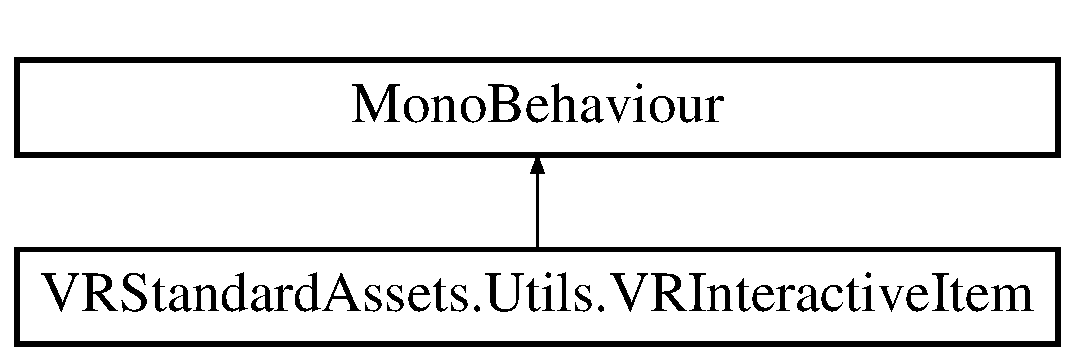
\includegraphics[height=2.000000cm]{class_v_r_standard_assets_1_1_utils_1_1_v_r_interactive_item}
\end{center}
\end{figure}
\subsection*{Public Member Functions}
\begin{DoxyCompactItemize}
\item 
void \mbox{\hyperlink{class_v_r_standard_assets_1_1_utils_1_1_v_r_interactive_item_a976794a3b7a35dad02dab0425d48a3ea}{Over}} ()
\item 
void \mbox{\hyperlink{class_v_r_standard_assets_1_1_utils_1_1_v_r_interactive_item_a7d7a426c71c0033399e4d3cf2957725d}{Out}} ()
\item 
void \mbox{\hyperlink{class_v_r_standard_assets_1_1_utils_1_1_v_r_interactive_item_a99c465d86dac6aee9da60e8fe158d481}{Click}} ()
\item 
void \mbox{\hyperlink{class_v_r_standard_assets_1_1_utils_1_1_v_r_interactive_item_a91b00f355ab0dcc33b57c454ba224381}{Double\+Click}} ()
\item 
void \mbox{\hyperlink{class_v_r_standard_assets_1_1_utils_1_1_v_r_interactive_item_aab8f0ab1f29eb9b8d5afdbde472cc7d3}{Up}} ()
\item 
void \mbox{\hyperlink{class_v_r_standard_assets_1_1_utils_1_1_v_r_interactive_item_afb9128eef421b2c35d4cc4b713d1e41a}{Down}} ()
\end{DoxyCompactItemize}
\subsection*{Protected Attributes}
\begin{DoxyCompactItemize}
\item 
bool \mbox{\hyperlink{class_v_r_standard_assets_1_1_utils_1_1_v_r_interactive_item_aac3eb76e3200547d20c7acb82a9882f8}{m\+\_\+\+Is\+Over}}
\end{DoxyCompactItemize}
\subsection*{Properties}
\begin{DoxyCompactItemize}
\item 
bool \mbox{\hyperlink{class_v_r_standard_assets_1_1_utils_1_1_v_r_interactive_item_adb4ca6b121df177d23e29a4a65710c88}{Is\+Over}}\hspace{0.3cm}{\ttfamily  \mbox{[}get\mbox{]}}
\end{DoxyCompactItemize}
\subsection*{Events}
\begin{DoxyCompactItemize}
\item 
Action \mbox{\hyperlink{class_v_r_standard_assets_1_1_utils_1_1_v_r_interactive_item_adf8b51724cbf6c291d87325b291cd629}{On\+Over}}
\item 
Action \mbox{\hyperlink{class_v_r_standard_assets_1_1_utils_1_1_v_r_interactive_item_aec12562b1b1948fed1a0367e15285921}{On\+Out}}
\item 
Action \mbox{\hyperlink{class_v_r_standard_assets_1_1_utils_1_1_v_r_interactive_item_a854b55cdbd774effd124fa7043c67d6e}{On\+Click}}
\item 
Action \mbox{\hyperlink{class_v_r_standard_assets_1_1_utils_1_1_v_r_interactive_item_a853961da1eba1b011ff7c511227ca0ba}{On\+Double\+Click}}
\item 
Action \mbox{\hyperlink{class_v_r_standard_assets_1_1_utils_1_1_v_r_interactive_item_af846c665a89a2b7859079d13d4c09147}{On\+Up}}
\item 
Action \mbox{\hyperlink{class_v_r_standard_assets_1_1_utils_1_1_v_r_interactive_item_a577be4607fd8102a068b50bafda3f032}{On\+Down}}
\end{DoxyCompactItemize}


\subsection{Member Function Documentation}
\mbox{\Hypertarget{class_v_r_standard_assets_1_1_utils_1_1_v_r_interactive_item_a99c465d86dac6aee9da60e8fe158d481}\label{class_v_r_standard_assets_1_1_utils_1_1_v_r_interactive_item_a99c465d86dac6aee9da60e8fe158d481}} 
\index{V\+R\+Standard\+Assets\+::\+Utils\+::\+V\+R\+Interactive\+Item@{V\+R\+Standard\+Assets\+::\+Utils\+::\+V\+R\+Interactive\+Item}!Click@{Click}}
\index{Click@{Click}!V\+R\+Standard\+Assets\+::\+Utils\+::\+V\+R\+Interactive\+Item@{V\+R\+Standard\+Assets\+::\+Utils\+::\+V\+R\+Interactive\+Item}}
\subsubsection{\texorpdfstring{Click()}{Click()}}
{\footnotesize\ttfamily void V\+R\+Standard\+Assets.\+Utils.\+V\+R\+Interactive\+Item.\+Click (\begin{DoxyParamCaption}{ }\end{DoxyParamCaption})}

\mbox{\Hypertarget{class_v_r_standard_assets_1_1_utils_1_1_v_r_interactive_item_a91b00f355ab0dcc33b57c454ba224381}\label{class_v_r_standard_assets_1_1_utils_1_1_v_r_interactive_item_a91b00f355ab0dcc33b57c454ba224381}} 
\index{V\+R\+Standard\+Assets\+::\+Utils\+::\+V\+R\+Interactive\+Item@{V\+R\+Standard\+Assets\+::\+Utils\+::\+V\+R\+Interactive\+Item}!Double\+Click@{Double\+Click}}
\index{Double\+Click@{Double\+Click}!V\+R\+Standard\+Assets\+::\+Utils\+::\+V\+R\+Interactive\+Item@{V\+R\+Standard\+Assets\+::\+Utils\+::\+V\+R\+Interactive\+Item}}
\subsubsection{\texorpdfstring{Double\+Click()}{DoubleClick()}}
{\footnotesize\ttfamily void V\+R\+Standard\+Assets.\+Utils.\+V\+R\+Interactive\+Item.\+Double\+Click (\begin{DoxyParamCaption}{ }\end{DoxyParamCaption})}

\mbox{\Hypertarget{class_v_r_standard_assets_1_1_utils_1_1_v_r_interactive_item_afb9128eef421b2c35d4cc4b713d1e41a}\label{class_v_r_standard_assets_1_1_utils_1_1_v_r_interactive_item_afb9128eef421b2c35d4cc4b713d1e41a}} 
\index{V\+R\+Standard\+Assets\+::\+Utils\+::\+V\+R\+Interactive\+Item@{V\+R\+Standard\+Assets\+::\+Utils\+::\+V\+R\+Interactive\+Item}!Down@{Down}}
\index{Down@{Down}!V\+R\+Standard\+Assets\+::\+Utils\+::\+V\+R\+Interactive\+Item@{V\+R\+Standard\+Assets\+::\+Utils\+::\+V\+R\+Interactive\+Item}}
\subsubsection{\texorpdfstring{Down()}{Down()}}
{\footnotesize\ttfamily void V\+R\+Standard\+Assets.\+Utils.\+V\+R\+Interactive\+Item.\+Down (\begin{DoxyParamCaption}{ }\end{DoxyParamCaption})}

\mbox{\Hypertarget{class_v_r_standard_assets_1_1_utils_1_1_v_r_interactive_item_a7d7a426c71c0033399e4d3cf2957725d}\label{class_v_r_standard_assets_1_1_utils_1_1_v_r_interactive_item_a7d7a426c71c0033399e4d3cf2957725d}} 
\index{V\+R\+Standard\+Assets\+::\+Utils\+::\+V\+R\+Interactive\+Item@{V\+R\+Standard\+Assets\+::\+Utils\+::\+V\+R\+Interactive\+Item}!Out@{Out}}
\index{Out@{Out}!V\+R\+Standard\+Assets\+::\+Utils\+::\+V\+R\+Interactive\+Item@{V\+R\+Standard\+Assets\+::\+Utils\+::\+V\+R\+Interactive\+Item}}
\subsubsection{\texorpdfstring{Out()}{Out()}}
{\footnotesize\ttfamily void V\+R\+Standard\+Assets.\+Utils.\+V\+R\+Interactive\+Item.\+Out (\begin{DoxyParamCaption}{ }\end{DoxyParamCaption})}

\mbox{\Hypertarget{class_v_r_standard_assets_1_1_utils_1_1_v_r_interactive_item_a976794a3b7a35dad02dab0425d48a3ea}\label{class_v_r_standard_assets_1_1_utils_1_1_v_r_interactive_item_a976794a3b7a35dad02dab0425d48a3ea}} 
\index{V\+R\+Standard\+Assets\+::\+Utils\+::\+V\+R\+Interactive\+Item@{V\+R\+Standard\+Assets\+::\+Utils\+::\+V\+R\+Interactive\+Item}!Over@{Over}}
\index{Over@{Over}!V\+R\+Standard\+Assets\+::\+Utils\+::\+V\+R\+Interactive\+Item@{V\+R\+Standard\+Assets\+::\+Utils\+::\+V\+R\+Interactive\+Item}}
\subsubsection{\texorpdfstring{Over()}{Over()}}
{\footnotesize\ttfamily void V\+R\+Standard\+Assets.\+Utils.\+V\+R\+Interactive\+Item.\+Over (\begin{DoxyParamCaption}{ }\end{DoxyParamCaption})}

\mbox{\Hypertarget{class_v_r_standard_assets_1_1_utils_1_1_v_r_interactive_item_aab8f0ab1f29eb9b8d5afdbde472cc7d3}\label{class_v_r_standard_assets_1_1_utils_1_1_v_r_interactive_item_aab8f0ab1f29eb9b8d5afdbde472cc7d3}} 
\index{V\+R\+Standard\+Assets\+::\+Utils\+::\+V\+R\+Interactive\+Item@{V\+R\+Standard\+Assets\+::\+Utils\+::\+V\+R\+Interactive\+Item}!Up@{Up}}
\index{Up@{Up}!V\+R\+Standard\+Assets\+::\+Utils\+::\+V\+R\+Interactive\+Item@{V\+R\+Standard\+Assets\+::\+Utils\+::\+V\+R\+Interactive\+Item}}
\subsubsection{\texorpdfstring{Up()}{Up()}}
{\footnotesize\ttfamily void V\+R\+Standard\+Assets.\+Utils.\+V\+R\+Interactive\+Item.\+Up (\begin{DoxyParamCaption}{ }\end{DoxyParamCaption})}



\subsection{Member Data Documentation}
\mbox{\Hypertarget{class_v_r_standard_assets_1_1_utils_1_1_v_r_interactive_item_aac3eb76e3200547d20c7acb82a9882f8}\label{class_v_r_standard_assets_1_1_utils_1_1_v_r_interactive_item_aac3eb76e3200547d20c7acb82a9882f8}} 
\index{V\+R\+Standard\+Assets\+::\+Utils\+::\+V\+R\+Interactive\+Item@{V\+R\+Standard\+Assets\+::\+Utils\+::\+V\+R\+Interactive\+Item}!m\+\_\+\+Is\+Over@{m\+\_\+\+Is\+Over}}
\index{m\+\_\+\+Is\+Over@{m\+\_\+\+Is\+Over}!V\+R\+Standard\+Assets\+::\+Utils\+::\+V\+R\+Interactive\+Item@{V\+R\+Standard\+Assets\+::\+Utils\+::\+V\+R\+Interactive\+Item}}
\subsubsection{\texorpdfstring{m\+\_\+\+Is\+Over}{m\_IsOver}}
{\footnotesize\ttfamily bool V\+R\+Standard\+Assets.\+Utils.\+V\+R\+Interactive\+Item.\+m\+\_\+\+Is\+Over\hspace{0.3cm}{\ttfamily [protected]}}



\subsection{Property Documentation}
\mbox{\Hypertarget{class_v_r_standard_assets_1_1_utils_1_1_v_r_interactive_item_adb4ca6b121df177d23e29a4a65710c88}\label{class_v_r_standard_assets_1_1_utils_1_1_v_r_interactive_item_adb4ca6b121df177d23e29a4a65710c88}} 
\index{V\+R\+Standard\+Assets\+::\+Utils\+::\+V\+R\+Interactive\+Item@{V\+R\+Standard\+Assets\+::\+Utils\+::\+V\+R\+Interactive\+Item}!Is\+Over@{Is\+Over}}
\index{Is\+Over@{Is\+Over}!V\+R\+Standard\+Assets\+::\+Utils\+::\+V\+R\+Interactive\+Item@{V\+R\+Standard\+Assets\+::\+Utils\+::\+V\+R\+Interactive\+Item}}
\subsubsection{\texorpdfstring{Is\+Over}{IsOver}}
{\footnotesize\ttfamily bool V\+R\+Standard\+Assets.\+Utils.\+V\+R\+Interactive\+Item.\+Is\+Over\hspace{0.3cm}{\ttfamily [get]}}



\subsection{Event Documentation}
\mbox{\Hypertarget{class_v_r_standard_assets_1_1_utils_1_1_v_r_interactive_item_a854b55cdbd774effd124fa7043c67d6e}\label{class_v_r_standard_assets_1_1_utils_1_1_v_r_interactive_item_a854b55cdbd774effd124fa7043c67d6e}} 
\index{V\+R\+Standard\+Assets\+::\+Utils\+::\+V\+R\+Interactive\+Item@{V\+R\+Standard\+Assets\+::\+Utils\+::\+V\+R\+Interactive\+Item}!On\+Click@{On\+Click}}
\index{On\+Click@{On\+Click}!V\+R\+Standard\+Assets\+::\+Utils\+::\+V\+R\+Interactive\+Item@{V\+R\+Standard\+Assets\+::\+Utils\+::\+V\+R\+Interactive\+Item}}
\subsubsection{\texorpdfstring{On\+Click}{OnClick}}
{\footnotesize\ttfamily Action V\+R\+Standard\+Assets.\+Utils.\+V\+R\+Interactive\+Item.\+On\+Click}

\mbox{\Hypertarget{class_v_r_standard_assets_1_1_utils_1_1_v_r_interactive_item_a853961da1eba1b011ff7c511227ca0ba}\label{class_v_r_standard_assets_1_1_utils_1_1_v_r_interactive_item_a853961da1eba1b011ff7c511227ca0ba}} 
\index{V\+R\+Standard\+Assets\+::\+Utils\+::\+V\+R\+Interactive\+Item@{V\+R\+Standard\+Assets\+::\+Utils\+::\+V\+R\+Interactive\+Item}!On\+Double\+Click@{On\+Double\+Click}}
\index{On\+Double\+Click@{On\+Double\+Click}!V\+R\+Standard\+Assets\+::\+Utils\+::\+V\+R\+Interactive\+Item@{V\+R\+Standard\+Assets\+::\+Utils\+::\+V\+R\+Interactive\+Item}}
\subsubsection{\texorpdfstring{On\+Double\+Click}{OnDoubleClick}}
{\footnotesize\ttfamily Action V\+R\+Standard\+Assets.\+Utils.\+V\+R\+Interactive\+Item.\+On\+Double\+Click}

\mbox{\Hypertarget{class_v_r_standard_assets_1_1_utils_1_1_v_r_interactive_item_a577be4607fd8102a068b50bafda3f032}\label{class_v_r_standard_assets_1_1_utils_1_1_v_r_interactive_item_a577be4607fd8102a068b50bafda3f032}} 
\index{V\+R\+Standard\+Assets\+::\+Utils\+::\+V\+R\+Interactive\+Item@{V\+R\+Standard\+Assets\+::\+Utils\+::\+V\+R\+Interactive\+Item}!On\+Down@{On\+Down}}
\index{On\+Down@{On\+Down}!V\+R\+Standard\+Assets\+::\+Utils\+::\+V\+R\+Interactive\+Item@{V\+R\+Standard\+Assets\+::\+Utils\+::\+V\+R\+Interactive\+Item}}
\subsubsection{\texorpdfstring{On\+Down}{OnDown}}
{\footnotesize\ttfamily Action V\+R\+Standard\+Assets.\+Utils.\+V\+R\+Interactive\+Item.\+On\+Down}

\mbox{\Hypertarget{class_v_r_standard_assets_1_1_utils_1_1_v_r_interactive_item_aec12562b1b1948fed1a0367e15285921}\label{class_v_r_standard_assets_1_1_utils_1_1_v_r_interactive_item_aec12562b1b1948fed1a0367e15285921}} 
\index{V\+R\+Standard\+Assets\+::\+Utils\+::\+V\+R\+Interactive\+Item@{V\+R\+Standard\+Assets\+::\+Utils\+::\+V\+R\+Interactive\+Item}!On\+Out@{On\+Out}}
\index{On\+Out@{On\+Out}!V\+R\+Standard\+Assets\+::\+Utils\+::\+V\+R\+Interactive\+Item@{V\+R\+Standard\+Assets\+::\+Utils\+::\+V\+R\+Interactive\+Item}}
\subsubsection{\texorpdfstring{On\+Out}{OnOut}}
{\footnotesize\ttfamily Action V\+R\+Standard\+Assets.\+Utils.\+V\+R\+Interactive\+Item.\+On\+Out}

\mbox{\Hypertarget{class_v_r_standard_assets_1_1_utils_1_1_v_r_interactive_item_adf8b51724cbf6c291d87325b291cd629}\label{class_v_r_standard_assets_1_1_utils_1_1_v_r_interactive_item_adf8b51724cbf6c291d87325b291cd629}} 
\index{V\+R\+Standard\+Assets\+::\+Utils\+::\+V\+R\+Interactive\+Item@{V\+R\+Standard\+Assets\+::\+Utils\+::\+V\+R\+Interactive\+Item}!On\+Over@{On\+Over}}
\index{On\+Over@{On\+Over}!V\+R\+Standard\+Assets\+::\+Utils\+::\+V\+R\+Interactive\+Item@{V\+R\+Standard\+Assets\+::\+Utils\+::\+V\+R\+Interactive\+Item}}
\subsubsection{\texorpdfstring{On\+Over}{OnOver}}
{\footnotesize\ttfamily Action V\+R\+Standard\+Assets.\+Utils.\+V\+R\+Interactive\+Item.\+On\+Over}

\mbox{\Hypertarget{class_v_r_standard_assets_1_1_utils_1_1_v_r_interactive_item_af846c665a89a2b7859079d13d4c09147}\label{class_v_r_standard_assets_1_1_utils_1_1_v_r_interactive_item_af846c665a89a2b7859079d13d4c09147}} 
\index{V\+R\+Standard\+Assets\+::\+Utils\+::\+V\+R\+Interactive\+Item@{V\+R\+Standard\+Assets\+::\+Utils\+::\+V\+R\+Interactive\+Item}!On\+Up@{On\+Up}}
\index{On\+Up@{On\+Up}!V\+R\+Standard\+Assets\+::\+Utils\+::\+V\+R\+Interactive\+Item@{V\+R\+Standard\+Assets\+::\+Utils\+::\+V\+R\+Interactive\+Item}}
\subsubsection{\texorpdfstring{On\+Up}{OnUp}}
{\footnotesize\ttfamily Action V\+R\+Standard\+Assets.\+Utils.\+V\+R\+Interactive\+Item.\+On\+Up}



The documentation for this class was generated from the following file\+:\begin{DoxyCompactItemize}
\item 
\mbox{\hyperlink{_v_r_interactive_item_8cs}{V\+R\+Interactive\+Item.\+cs}}\end{DoxyCompactItemize}

\hypertarget{class_v_r_standard_assets_1_1_utils_1_1_v_r_tracking_reset}{}\section{V\+R\+Standard\+Assets.\+Utils.\+V\+R\+Tracking\+Reset Class Reference}
\label{class_v_r_standard_assets_1_1_utils_1_1_v_r_tracking_reset}\index{V\+R\+Standard\+Assets.\+Utils.\+V\+R\+Tracking\+Reset@{V\+R\+Standard\+Assets.\+Utils.\+V\+R\+Tracking\+Reset}}
Inheritance diagram for V\+R\+Standard\+Assets.\+Utils.\+V\+R\+Tracking\+Reset\+:\begin{figure}[H]
\begin{center}
\leavevmode
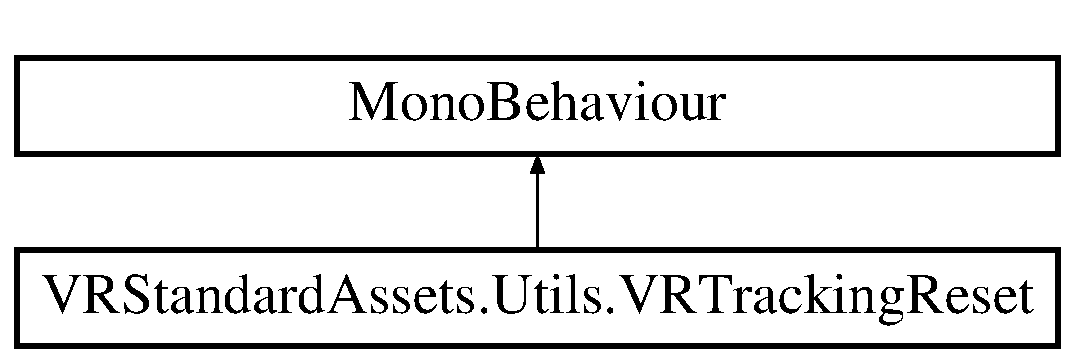
\includegraphics[height=2.000000cm]{class_v_r_standard_assets_1_1_utils_1_1_v_r_tracking_reset}
\end{center}
\end{figure}
\subsection*{Private Member Functions}
\begin{DoxyCompactItemize}
\item 
void \mbox{\hyperlink{class_v_r_standard_assets_1_1_utils_1_1_v_r_tracking_reset_ac44c9cb15949558a8a3fa93bbb7c7e83}{On\+Application\+Pause}} (bool pause\+Status)
\end{DoxyCompactItemize}


\subsection{Member Function Documentation}
\mbox{\Hypertarget{class_v_r_standard_assets_1_1_utils_1_1_v_r_tracking_reset_ac44c9cb15949558a8a3fa93bbb7c7e83}\label{class_v_r_standard_assets_1_1_utils_1_1_v_r_tracking_reset_ac44c9cb15949558a8a3fa93bbb7c7e83}} 
\index{V\+R\+Standard\+Assets\+::\+Utils\+::\+V\+R\+Tracking\+Reset@{V\+R\+Standard\+Assets\+::\+Utils\+::\+V\+R\+Tracking\+Reset}!On\+Application\+Pause@{On\+Application\+Pause}}
\index{On\+Application\+Pause@{On\+Application\+Pause}!V\+R\+Standard\+Assets\+::\+Utils\+::\+V\+R\+Tracking\+Reset@{V\+R\+Standard\+Assets\+::\+Utils\+::\+V\+R\+Tracking\+Reset}}
\subsubsection{\texorpdfstring{On\+Application\+Pause()}{OnApplicationPause()}}
{\footnotesize\ttfamily void V\+R\+Standard\+Assets.\+Utils.\+V\+R\+Tracking\+Reset.\+On\+Application\+Pause (\begin{DoxyParamCaption}\item[{bool}]{pause\+Status }\end{DoxyParamCaption})\hspace{0.3cm}{\ttfamily [private]}}



The documentation for this class was generated from the following file\+:\begin{DoxyCompactItemize}
\item 
\mbox{\hyperlink{_v_r_tracking_reset_8cs}{V\+R\+Tracking\+Reset.\+cs}}\end{DoxyCompactItemize}

\chapter{File Documentation}
\hypertarget{_ball_controls_8cs}{}\section{Ball\+Controls.\+cs File Reference}
\label{_ball_controls_8cs}\index{Ball\+Controls.\+cs@{Ball\+Controls.\+cs}}
\subsection*{Classes}
\begin{DoxyCompactItemize}
\item 
class \mbox{\hyperlink{class_ball_controls}{Ball\+Controls}}
\end{DoxyCompactItemize}

\hypertarget{_dialogue_asset_8cs}{}\section{Dialogue/\+Editor/\+Dialogue\+Asset.cs File Reference}
\label{_dialogue_asset_8cs}\index{Dialogue/\+Editor/\+Dialogue\+Asset.\+cs@{Dialogue/\+Editor/\+Dialogue\+Asset.\+cs}}
\subsection*{Classes}
\begin{DoxyCompactItemize}
\item 
class \mbox{\hyperlink{class_dialogue_asset}{Dialogue\+Asset}}
\begin{DoxyCompactList}\small\item\em Overload the menu for creating a custom \mbox{\hyperlink{class_dialogue}{Dialogue}} asset. \end{DoxyCompactList}\end{DoxyCompactItemize}

\hypertarget{_dialogue_editor_8cs}{}\section{Dialogue/\+Editor/\+Dialogue\+Editor.cs File Reference}
\label{_dialogue_editor_8cs}\index{Dialogue/\+Editor/\+Dialogue\+Editor.\+cs@{Dialogue/\+Editor/\+Dialogue\+Editor.\+cs}}
\subsection*{Classes}
\begin{DoxyCompactItemize}
\item 
class \mbox{\hyperlink{class_dialogue_editor}{Dialogue\+Editor}}
\begin{DoxyCompactList}\small\item\em Tells Unity that we can handle the editor view ourself. \end{DoxyCompactList}\end{DoxyCompactItemize}

\hypertarget{_custom_asset_utility_8cs}{}\section{Dialogue/scripts/\+Custom\+Asset\+Utility.cs File Reference}
\label{_custom_asset_utility_8cs}\index{Dialogue/scripts/\+Custom\+Asset\+Utility.\+cs@{Dialogue/scripts/\+Custom\+Asset\+Utility.\+cs}}

\hypertarget{_dialogue_8cs}{}\section{Dialogue/scripts/\+Dialogue.cs File Reference}
\label{_dialogue_8cs}\index{Dialogue/scripts/\+Dialogue.\+cs@{Dialogue/scripts/\+Dialogue.\+cs}}
\subsection*{Classes}
\begin{DoxyCompactItemize}
\item 
class \mbox{\hyperlink{class_dialogue}{Dialogue}}
\begin{DoxyCompactList}\small\item\em Creates a List of elements which contain attributes from \mbox{\hyperlink{_dialogue_element_8cs}{Dialogue\+Element.\+cs}} \end{DoxyCompactList}\end{DoxyCompactItemize}

\hypertarget{_dialogue_element_8cs}{}\section{Dialogue/scripts/\+Dialogue\+Element.cs File Reference}
\label{_dialogue_element_8cs}\index{Dialogue/scripts/\+Dialogue\+Element.\+cs@{Dialogue/scripts/\+Dialogue\+Element.\+cs}}
\subsection*{Classes}
\begin{DoxyCompactItemize}
\item 
class \mbox{\hyperlink{class_dialogue_element}{Dialogue\+Element}}
\begin{DoxyCompactList}\small\item\em This is where you can add attributes to each dialogue element instance. Note some of this wasn\textquotesingle{}t used or included in the \mbox{\hyperlink{class_dialogue_editor}{Dialogue\+Editor}} view under Project $>$ \mbox{\hyperlink{class_dialogue}{Dialogue}} $>$ Editor... \end{DoxyCompactList}\end{DoxyCompactItemize}

\hypertarget{_end_scene_8cs}{}\section{End\+Scene.\+cs File Reference}
\label{_end_scene_8cs}\index{End\+Scene.\+cs@{End\+Scene.\+cs}}
\subsection*{Classes}
\begin{DoxyCompactItemize}
\item 
class \mbox{\hyperlink{class_end_scene}{End\+Scene}}
\end{DoxyCompactItemize}

\hypertarget{_flip_normals_8cs}{}\section{Flip\+Normals.\+cs File Reference}
\label{_flip_normals_8cs}\index{Flip\+Normals.\+cs@{Flip\+Normals.\+cs}}
\subsection*{Classes}
\begin{DoxyCompactItemize}
\item 
class \mbox{\hyperlink{class_flip_normals}{Flip\+Normals}}
\begin{DoxyCompactList}\small\item\em Use this to invert the normals of an object \end{DoxyCompactList}\end{DoxyCompactItemize}

\hypertarget{_force_field_8cs}{}\section{Force\+Field.\+cs File Reference}
\label{_force_field_8cs}\index{Force\+Field.\+cs@{Force\+Field.\+cs}}
\subsection*{Classes}
\begin{DoxyCompactItemize}
\item 
class \mbox{\hyperlink{class_force_field}{Force\+Field}}
\begin{DoxyCompactList}\small\item\em Class is used to destroy objects when they are thrown too far This is done by determining when the object exits the forcefield (On\+Trigger\+Exit) and when that happens it will be destroyed. \end{DoxyCompactList}\end{DoxyCompactItemize}

\hypertarget{_intro_session_manager_8cs}{}\section{Intro\+Session\+Manager.\+cs File Reference}
\label{_intro_session_manager_8cs}\index{Intro\+Session\+Manager.\+cs@{Intro\+Session\+Manager.\+cs}}
\subsection*{Classes}
\begin{DoxyCompactItemize}
\item 
class \mbox{\hyperlink{class_intro_session_manager}{Intro\+Session\+Manager}}
\end{DoxyCompactItemize}

\hypertarget{_move_robot_8cs}{}\section{Move\+Robot.\+cs File Reference}
\label{_move_robot_8cs}\index{Move\+Robot.\+cs@{Move\+Robot.\+cs}}
\subsection*{Classes}
\begin{DoxyCompactItemize}
\item 
class \mbox{\hyperlink{class_move_robot}{Move\+Robot}}
\end{DoxyCompactItemize}

\hypertarget{_raycaster_v_r_8cs}{}\section{Raycaster\+V\+R.\+cs File Reference}
\label{_raycaster_v_r_8cs}\index{Raycaster\+V\+R.\+cs@{Raycaster\+V\+R.\+cs}}
\subsection*{Classes}
\begin{DoxyCompactItemize}
\item 
class \mbox{\hyperlink{class_v_r_standard_assets_1_1_utils_1_1_raycaster_v_r}{V\+R\+Standard\+Assets.\+Utils.\+Raycaster\+VR}}
\end{DoxyCompactItemize}
\subsection*{Namespaces}
\begin{DoxyCompactItemize}
\item 
namespace \mbox{\hyperlink{namespace_v_r_standard_assets_1_1_utils}{V\+R\+Standard\+Assets.\+Utils}}
\end{DoxyCompactItemize}

\hypertarget{_reticle_8cs}{}\section{Reticle.\+cs File Reference}
\label{_reticle_8cs}\index{Reticle.\+cs@{Reticle.\+cs}}
\subsection*{Classes}
\begin{DoxyCompactItemize}
\item 
class \mbox{\hyperlink{class_v_r_standard_assets_1_1_utils_1_1_reticle}{V\+R\+Standard\+Assets.\+Utils.\+Reticle}}
\end{DoxyCompactItemize}
\subsection*{Namespaces}
\begin{DoxyCompactItemize}
\item 
namespace \mbox{\hyperlink{namespace_v_r_standard_assets_1_1_utils}{V\+R\+Standard\+Assets.\+Utils}}
\end{DoxyCompactItemize}

\hypertarget{_stage1_8cs}{}\section{Stage1.\+cs File Reference}
\label{_stage1_8cs}\index{Stage1.\+cs@{Stage1.\+cs}}
\subsection*{Classes}
\begin{DoxyCompactItemize}
\item 
class \mbox{\hyperlink{class_stage1}{Stage1}}
\end{DoxyCompactItemize}

\hypertarget{_stage2_8cs}{}\section{Stage2.\+cs File Reference}
\label{_stage2_8cs}\index{Stage2.\+cs@{Stage2.\+cs}}
\subsection*{Classes}
\begin{DoxyCompactItemize}
\item 
class \mbox{\hyperlink{class_stage2}{Stage2}}
\end{DoxyCompactItemize}

\hypertarget{_stage3_8cs}{}\section{Stage3.\+cs File Reference}
\label{_stage3_8cs}\index{Stage3.\+cs@{Stage3.\+cs}}
\subsection*{Classes}
\begin{DoxyCompactItemize}
\item 
class \mbox{\hyperlink{class_stage3}{Stage3}}
\end{DoxyCompactItemize}

\hypertarget{_stage4_8cs}{}\section{Stage4.\+cs File Reference}
\label{_stage4_8cs}\index{Stage4.\+cs@{Stage4.\+cs}}
\subsection*{Classes}
\begin{DoxyCompactItemize}
\item 
class \mbox{\hyperlink{class_stage4}{Stage4}}
\end{DoxyCompactItemize}

\hypertarget{_stage5_8cs}{}\section{Stage5.\+cs File Reference}
\label{_stage5_8cs}\index{Stage5.\+cs@{Stage5.\+cs}}
\subsection*{Classes}
\begin{DoxyCompactItemize}
\item 
class \mbox{\hyperlink{class_stage5}{Stage5}}
\end{DoxyCompactItemize}

\hypertarget{_stage6_8cs}{}\section{Stage6.\+cs File Reference}
\label{_stage6_8cs}\index{Stage6.\+cs@{Stage6.\+cs}}
\subsection*{Classes}
\begin{DoxyCompactItemize}
\item 
class \mbox{\hyperlink{class_stage6}{Stage6}}
\end{DoxyCompactItemize}

\hypertarget{_target_8cs}{}\section{Target.\+cs File Reference}
\label{_target_8cs}\index{Target.\+cs@{Target.\+cs}}
\subsection*{Classes}
\begin{DoxyCompactItemize}
\item 
class \mbox{\hyperlink{class_target}{Target}}
\begin{DoxyCompactList}\small\item\em Class is designed to be used on the targets in Scene6. They have a voxel effect when they are hit by the ball. \end{DoxyCompactList}\end{DoxyCompactItemize}

\hypertarget{_trigger_stage4_8cs}{}\section{Trigger\+Stage4.\+cs File Reference}
\label{_trigger_stage4_8cs}\index{Trigger\+Stage4.\+cs@{Trigger\+Stage4.\+cs}}
\subsection*{Classes}
\begin{DoxyCompactItemize}
\item 
class \mbox{\hyperlink{class_trigger_stage4}{Trigger\+Stage4}}
\begin{DoxyCompactList}\small\item\em Class is designed for Scene4 to be listening for when an object is dropped through the doors \end{DoxyCompactList}\end{DoxyCompactItemize}

\hypertarget{_v_r_camera_u_i_8cs}{}\section{V\+R\+Camera\+U\+I.\+cs File Reference}
\label{_v_r_camera_u_i_8cs}\index{V\+R\+Camera\+U\+I.\+cs@{V\+R\+Camera\+U\+I.\+cs}}
\subsection*{Classes}
\begin{DoxyCompactItemize}
\item 
class \mbox{\hyperlink{class_v_r_standard_assets_1_1_utils_1_1_v_r_camera_u_i}{V\+R\+Standard\+Assets.\+Utils.\+V\+R\+Camera\+UI}}
\end{DoxyCompactItemize}
\subsection*{Namespaces}
\begin{DoxyCompactItemize}
\item 
namespace \mbox{\hyperlink{namespace_v_r_standard_assets_1_1_utils}{V\+R\+Standard\+Assets.\+Utils}}
\end{DoxyCompactItemize}

\hypertarget{_v_r_device_manager_8cs}{}\section{V\+R\+Device\+Manager.\+cs File Reference}
\label{_v_r_device_manager_8cs}\index{V\+R\+Device\+Manager.\+cs@{V\+R\+Device\+Manager.\+cs}}
\subsection*{Classes}
\begin{DoxyCompactItemize}
\item 
class \mbox{\hyperlink{class_v_r_standard_assets_1_1_utils_1_1_v_r_device_manager}{V\+R\+Standard\+Assets.\+Utils.\+V\+R\+Device\+Manager}}
\end{DoxyCompactItemize}
\subsection*{Namespaces}
\begin{DoxyCompactItemize}
\item 
namespace \mbox{\hyperlink{namespace_v_r_standard_assets_1_1_utils}{V\+R\+Standard\+Assets.\+Utils}}
\end{DoxyCompactItemize}

\hypertarget{_v_r_input_8cs}{}\section{V\+R\+Input.\+cs File Reference}
\label{_v_r_input_8cs}\index{V\+R\+Input.\+cs@{V\+R\+Input.\+cs}}
\subsection*{Classes}
\begin{DoxyCompactItemize}
\item 
class \mbox{\hyperlink{class_v_r_standard_assets_1_1_utils_1_1_v_r_input}{V\+R\+Standard\+Assets.\+Utils.\+V\+R\+Input}}
\end{DoxyCompactItemize}
\subsection*{Namespaces}
\begin{DoxyCompactItemize}
\item 
namespace \mbox{\hyperlink{namespace_v_r_standard_assets_1_1_utils}{V\+R\+Standard\+Assets.\+Utils}}
\end{DoxyCompactItemize}

\hypertarget{_v_r_interactive_item_8cs}{}\section{V\+R\+Interactive\+Item.\+cs File Reference}
\label{_v_r_interactive_item_8cs}\index{V\+R\+Interactive\+Item.\+cs@{V\+R\+Interactive\+Item.\+cs}}
\subsection*{Classes}
\begin{DoxyCompactItemize}
\item 
class \mbox{\hyperlink{class_v_r_standard_assets_1_1_utils_1_1_v_r_interactive_item}{V\+R\+Standard\+Assets.\+Utils.\+V\+R\+Interactive\+Item}}
\end{DoxyCompactItemize}
\subsection*{Namespaces}
\begin{DoxyCompactItemize}
\item 
namespace \mbox{\hyperlink{namespace_v_r_standard_assets_1_1_utils}{V\+R\+Standard\+Assets.\+Utils}}
\end{DoxyCompactItemize}

\hypertarget{_v_r_tracking_reset_8cs}{}\section{V\+R\+Tracking\+Reset.\+cs File Reference}
\label{_v_r_tracking_reset_8cs}\index{V\+R\+Tracking\+Reset.\+cs@{V\+R\+Tracking\+Reset.\+cs}}
\subsection*{Classes}
\begin{DoxyCompactItemize}
\item 
class \mbox{\hyperlink{class_v_r_standard_assets_1_1_utils_1_1_v_r_tracking_reset}{V\+R\+Standard\+Assets.\+Utils.\+V\+R\+Tracking\+Reset}}
\end{DoxyCompactItemize}
\subsection*{Namespaces}
\begin{DoxyCompactItemize}
\item 
namespace \mbox{\hyperlink{namespace_v_r_standard_assets_1_1_utils}{V\+R\+Standard\+Assets.\+Utils}}
\end{DoxyCompactItemize}

%--- End generated contents ---

% Index
\backmatter
\newpage
\phantomsection
\clearemptydoublepage
\addcontentsline{toc}{chapter}{Index}
\printindex

\end{document}
